%-*-latex-*-
\mychapter{106}{5400}{Trees}

\newpage%-*-latex-*-
\sectionthree{Tree}
\begin{python0}
from solutions import *; clear()
\end{python0}

A tree is just a connected graph without cycles.
In this case, I'm talking about a tree as an undirected
graph.
You have to be careful, sometimes, a tree can also 
refer to a tree as a directed graph and acyclic.

Sometimes a special node is selected.
In this case, such a tree is sometimes called a rooted tree
(or a tree with a root).

Here's a tree (directed version):


\begin{center}
\begin{tikzpicture}[>=triangle 60,shorten >=0.5pt,node distance=2cm,auto,initial text=, double distance=2pt]
\node[state] (A) at (  3,  0) {$A$};
\node[state] (B) at (  6,  0) {$B$};
\node[state] (S) at (  0, -2) {$S$};
\node[state] (C) at (  3, -4) {$C$};

\path[->]
(A) edge [bend left=0,pos=0.5,above] node {} (B)
(A) edge [bend left=0,pos=0.5] node {} (C)
(S) edge [bend left=0,pos=0.5,above] node {} (A)
(S) edge [bend left=0,pos=0.5,above] node {} (C)

;
\end{tikzpicture}
\end{center}
    


\begin{myenum}

  \li
  $a$ is the \defone{root} of the tree.

  \li
  $a$ has 3 \defone{children}, i.e., $b,c,d$; 
  $a$ has a
  \sidebarskip{8pt}
  \defone{branching factor} 
  of 3.
  Sometimes, it's convenient to number the children.
  I'll call $b$ child $0$ of $a$; $d$ is child $2$ of $a$.

  \li
  $a$ is the \defone{parent} of $b$.

  \li
  $k$,$l$,$f$,$g$,$m$,$i$,$j$ are called
  \sidebarskip{-2pt}
  \defone{leaves}
  or
  \sidebarskip{12pt}\defone{non-internal} nodes because
  they don't have children.

  \li
  $a,b,c,d,e,h$ are called
  \sidebarskip{-2pt}
  \defone{non-leaf} nodes or 
  \sidebarskip{12pt}\defone{internal} nodes because 
  each have at least one child.

  \li
  $b$ has a \defone{depth} of $1$, i.e., 
  the length of the path from the root to $b$
  is 1. I will also say that $b$ is at level $1$.
  A root (see $a$ above) has depth 0.

  \li
  $b$ has a \defone{height} of $2$, i.e., 
  the length of the longest path from 
  $b$ to a leaf is 2.
  A leaf (see $k$ above) has height 0.

  \li
  The \defone{height} of a tree is the height of the root of the tree.
  The above tree has a height of 3.
  The height of an empty tree is -1.

  \li
  The root is at level 0. $b,c,d$ are at level 1.
  $e,f,g,h,i,j$ are at level 2. $k,l,m$ are at level 3.
  
  \li
  Two nodes $u$ and $v$ are \defone{siblings} if they have
  the same parent.
  For instance $b,c,d$ are siblings.
  
  \li
  $u$ has \defone{descendent} $v$ if there is a sequence of nodes 
  $u = v_0$, $v_1$, ..., $v_n = v$ where $v_i$ is the parent of $v_{i+1}$.
  $v$ is the \defone{ancestor} of $u$ if $u$ is a descendent of $v$.
  For instance in the above tree $b$ is an ancestor of $i$ and
  $i$ is a descendent of $l$.

\end{myenum}
Note that the above tree is a directed graph.
The following is also a tree (as in an \textit{undirected} tree).

%-*-latex-*-
{\footnotesize \begin{Verbatim}[frame=single,fontsize=\small]
[student@localhost discrete-probability] python tossfaircoin2.py
experiment 0 ... outcome: TAIL
experiment 1 ... outcome: TAIL
experiment 2 ... outcome: TAIL
experiment 3 ... outcome: TAIL
experiment 4 ... outcome: TAIL
experiment 5 ... outcome: TAIL
experiment 6 ... outcome: HEAD
experiment 7 ... outcome: TAIL
experiment 8 ... outcome: TAIL
experiment 9 ... outcome: TAIL
experiment 10 ... outcome: TAIL
experiment 11 ... outcome: HEAD
experiment 12 ... outcome: HEAD
experiment 13 ... outcome: TAIL
experiment 14 ... outcome: HEAD
experiment 15 ... outcome: TAIL
experiment 16 ... outcome: TAIL
experiment 17 ... outcome: HEAD
experiment 18 ... outcome: HEAD
experiment 19 ... outcome: TAIL
number of experiments: 20
number of heads: 6
number of tails: 14
probability of getting head: 0.3
probability of getting tail: 0.7
\end{Verbatim}
}


In the case of implementation, you can think of the directed version
as having pointers from a parent to the children.
In the case of the undirected version, you can think of
each edge as allowing you to go both up and down -- 
nodes having pointers going to their children or parent.
Of course exceptions being that roots have no parents and leaves have no
children.

For each node of a tree $T$, if you consider all the descendents of the node, 
you have a tree. This is called a \defone{subtree} of $T$.
For instance

\begin{console}
12094
\end{console}


is a subtree of 

\begin{center}
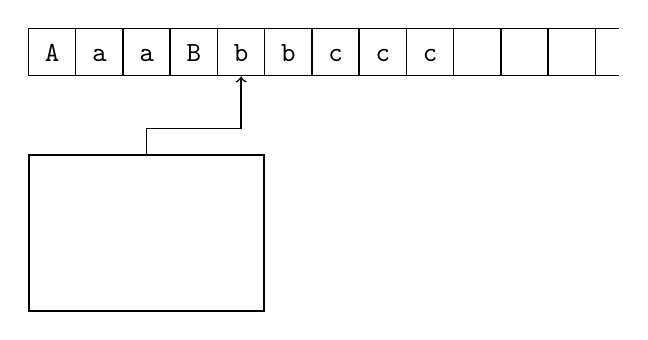
\begin{tikzpicture}

\draw (0.3, 0.3)
  node[draw, line width=0.02cm, , color=black,
       rounded corners=0cm, inner sep=0cm] {

\begin{minipage}[t][0.6cm]{0.6cm}
\mbox{}

\end{minipage}

};\draw (0.3, 0.3) node[color=black] {{\vphantom{AaaBbbccc$\BLANK$$\BLANK$$\BLANK$}\texttt{A}}};
\draw (0.8999999999999999, 0.3)
  node[draw, line width=0.02cm, , color=black,
       rounded corners=0cm, inner sep=0cm] {

\begin{minipage}[t][0.6cm]{0.6cm}
\mbox{}

\end{minipage}

};\draw (0.8999999999999999, 0.3) node[color=black] {{\vphantom{AaaBbbccc$\BLANK$$\BLANK$$\BLANK$}\texttt{a}}};
\draw (1.5, 0.3)
  node[draw, line width=0.02cm, , color=black,
       rounded corners=0cm, inner sep=0cm] {

\begin{minipage}[t][0.6cm]{0.6cm}
\mbox{}

\end{minipage}

};\draw (1.5, 0.3) node[color=black] {{\vphantom{AaaBbbccc$\BLANK$$\BLANK$$\BLANK$}\texttt{a}}};
\draw (2.0999999999999996, 0.3)
  node[draw, line width=0.02cm, , color=black,
       rounded corners=0cm, inner sep=0cm] {

\begin{minipage}[t][0.6cm]{0.6cm}
\mbox{}

\end{minipage}

};\draw (2.0999999999999996, 0.3) node[color=black] {{\vphantom{AaaBbbccc$\BLANK$$\BLANK$$\BLANK$}\texttt{B}}};
\draw (2.7, 0.3)
  node[draw, line width=0.02cm, , color=black,
       rounded corners=0cm, inner sep=0cm] {

\begin{minipage}[t][0.6cm]{0.6cm}
\mbox{}

\end{minipage}

};\draw (2.7, 0.3) node[color=black] {{\vphantom{AaaBbbccc$\BLANK$$\BLANK$$\BLANK$}\texttt{b}}};
\draw (3.3, 0.3)
  node[draw, line width=0.02cm, , color=black,
       rounded corners=0cm, inner sep=0cm] {

\begin{minipage}[t][0.6cm]{0.6cm}
\mbox{}

\end{minipage}

};\draw (3.3, 0.3) node[color=black] {{\vphantom{AaaBbbccc$\BLANK$$\BLANK$$\BLANK$}\texttt{b}}};
\draw (3.9000000000000004, 0.3)
  node[draw, line width=0.02cm, , color=black,
       rounded corners=0cm, inner sep=0cm] {

\begin{minipage}[t][0.6cm]{0.6cm}
\mbox{}

\end{minipage}

};\draw (3.9000000000000004, 0.3) node[color=black] {{\vphantom{AaaBbbccc$\BLANK$$\BLANK$$\BLANK$}\texttt{c}}};
\draw (4.5, 0.3)
  node[draw, line width=0.02cm, , color=black,
       rounded corners=0cm, inner sep=0cm] {

\begin{minipage}[t][0.6cm]{0.6cm}
\mbox{}

\end{minipage}

};\draw (4.5, 0.3) node[color=black] {{\vphantom{AaaBbbccc$\BLANK$$\BLANK$$\BLANK$}\texttt{c}}};
\draw (5.1, 0.3)
  node[draw, line width=0.02cm, , color=black,
       rounded corners=0cm, inner sep=0cm] {

\begin{minipage}[t][0.6cm]{0.6cm}
\mbox{}

\end{minipage}

};\draw (5.1, 0.3) node[color=black] {{\vphantom{AaaBbbccc$\BLANK$$\BLANK$$\BLANK$}\texttt{c}}};
\draw (5.699999999999999, 0.3)
  node[draw, line width=0.02cm, , color=black,
       rounded corners=0cm, inner sep=0cm] {

\begin{minipage}[t][0.6cm]{0.6cm}
\mbox{}

\end{minipage}

};\draw (5.699999999999999, 0.3) node[color=black] {{\vphantom{AaaBbbccc$\BLANK$$\BLANK$$\BLANK$}\texttt{$\BLANK$}}};
\draw (6.299999999999999, 0.3)
  node[draw, line width=0.02cm, , color=black,
       rounded corners=0cm, inner sep=0cm] {

\begin{minipage}[t][0.6cm]{0.6cm}
\mbox{}

\end{minipage}

};\draw (6.299999999999999, 0.3) node[color=black] {{\vphantom{AaaBbbccc$\BLANK$$\BLANK$$\BLANK$}\texttt{$\BLANK$}}};
\draw (6.899999999999999, 0.3)
  node[draw, line width=0.02cm, , color=black,
       rounded corners=0cm, inner sep=0cm] {

\begin{minipage}[t][0.6cm]{0.6cm}
\mbox{}

\end{minipage}

};\draw (6.899999999999999, 0.3) node[color=black] {{\vphantom{AaaBbbccc$\BLANK$$\BLANK$$\BLANK$}\texttt{$\BLANK$}}};\draw[line width=0.02cm,black] (7.1999999999999975,0.6) to  (7.499999999999998,0.6);
\draw[line width=0.02cm,black] (7.1999999999999975,0.0) to  (7.499999999999998,0.0);

\draw (1.5, -2.0)
  node[draw, line width=0.02cm, , color=black,
       rounded corners=0cm, inner sep=0cm] {

\begin{minipage}[t][1.98cm]{2.98cm}
\mbox{}

\end{minipage}

};\draw[line width=0.02cm,black,->] (1.5,-1) to  (1.5,-0.67) to  (2.7,-0.67) to  (2.7,-0.01);
\end{tikzpicture}

\end{center}



I will say that this is the subtree at $b$.

In the case of a node with two child, 
there are two subtrees, the subtree on the left is called the 
\defone{left subtree} and the one on the right is called the 
\defone{right subtree}.
(Duh.)
Look at the subtree at $b$:

%-*-latex-*-
\begin{Verbatim}[frame=single,fontsize=\small]
[student@localhost discrete-probability] python discrete-probrobability/game2.py
python: can't open file 'discrete-probrobability/game2.py': [Errno 2] No such fi
le or directory
\end{Verbatim}



The nodes $e,k,l$ form the left subtree of $b$
and the single node $f$ form the right subtree of $b$.


A tree is said to be \defone{$k$--ary} if every node has at most $k$ children;
that's the same as saying that every node has a maximum branching factor of
$k$.
In particular, a \defone{binary} tree is a tree with at most 2 children.


\begin{ex} 
  \label{ex:some-decision1}
  \tinysidebar{\debug{exercises/{empty0/question.tex}}}
  \solutionlink{sol:some-decision1}
  \qed
\end{ex} 
\begin{python0}
from solutions import *
add(label="ex:some-decision1",
    srcfilename='exercises/some-decision1/answer.tex') 
\end{python0}


We include the empty graph as a tree, except of course such trees
don't have roots.
Consider a $k$--ary tree $T$.
\begin{myenum}

\li $T$ is \defone{full} if every node has exactly $k$ children, except for 
the leaves, i.e., if every node has
either $k$ or $0$ children.
Here's a full binary tree:

\begin{center}
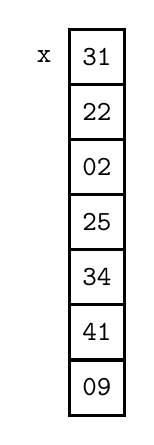
\begin{tikzpicture}

\draw (0.35, -0.35)
  node[draw, line width=0.04cm, , color=black,
       rounded corners=0cm, inner sep=0cm] {

\begin{minipage}[t][0.7cm]{0.7cm}
\mbox{}

\end{minipage}

};\draw (0.35, -0.35) node[color=black] {{\texttt{31}}};
\draw (0.35, -1.0499999999999998)
  node[draw, line width=0.04cm, , color=black,
       rounded corners=0cm, inner sep=0cm] {

\begin{minipage}[t][0.7cm]{0.7cm}
\mbox{}

\end{minipage}

};\draw (0.35, -1.0499999999999998) node[color=black] {{\texttt{22}}};
\draw (0.35, -1.7499999999999996)
  node[draw, line width=0.04cm, , color=black,
       rounded corners=0cm, inner sep=0cm] {

\begin{minipage}[t][0.7cm]{0.7cm}
\mbox{}

\end{minipage}

};\draw (0.35, -1.7499999999999996) node[color=black] {{\texttt{02}}};
\draw (0.35, -2.4499999999999997)
  node[draw, line width=0.04cm, , color=black,
       rounded corners=0cm, inner sep=0cm] {

\begin{minipage}[t][0.7cm]{0.7cm}
\mbox{}

\end{minipage}

};\draw (0.35, -2.4499999999999997) node[color=black] {{\texttt{25}}};
\draw (0.35, -3.15)
  node[draw, line width=0.04cm, , color=black,
       rounded corners=0cm, inner sep=0cm] {

\begin{minipage}[t][0.7cm]{0.7cm}
\mbox{}

\end{minipage}

};\draw (0.35, -3.15) node[color=black] {{\texttt{34}}};
\draw (0.35, -3.8499999999999996)
  node[draw, line width=0.04cm, , color=black,
       rounded corners=0cm, inner sep=0cm] {

\begin{minipage}[t][0.7cm]{0.7cm}
\mbox{}

\end{minipage}

};\draw (0.35, -3.8499999999999996) node[color=black] {{\texttt{41}}};
\draw (0.35, -4.550000000000001)
  node[draw, line width=0.04cm, , color=black,
       rounded corners=0cm, inner sep=0cm] {

\begin{minipage}[t][0.7cm]{0.7cm}
\mbox{}

\end{minipage}

};\draw (0.35, -4.550000000000001) node[color=black] {{\texttt{09}}};
\draw (-0.32, -0.35)
  node[draw=none, line width=0cm, , color=black,
       rounded corners=0cm, inner sep=0cm] {

\begin{minipage}[t][0.1cm]{0.1cm}
\mbox{}

\end{minipage}

};\draw (-0.32, -0.35) node[color=black] {\text{\texttt{x}}};
\end{tikzpicture}

\end{center}



Here's another:

\begin{console}[frame=single, , commandchars=~@$]
SLNode * p = phead;
while (p != NULL)
{
    std::cout << (*p) << std::endl;
    p = p->next();
}
\end{console}

and the output is this:
\begin{console}[frame=single,fontsize=\footnotesize]
[student@localhost linkedlist] g++ tmp12345678.cpp; ./a.out
<SLNode 0x7ffcf03deca0 key:2, next:0x7ffcf03decb0>
<SLNode 0x7ffcf03decb0 key:6, next:0x7ffcf03decc0>
<SLNode 0x7ffcf03decc0 key:4, next:0x7ffcf03decd0>
<SLNode 0x7ffcf03decd0 key:5, next:0>
\end{console}



\li $T$ is \defone{perfect} if $T$ is full and the leaves are 
at the same level.
Here's a perfect binary tree:


\begin{longtable}{|r||r|r|r|r|r|}
\hline 
         & $0$ & $1$ & $2$ & $3$ & $\ldots$ \\ \hline \hline 
$x_0$    & 5   & 0   & 0   & 0   & ...      \\ \hline 
$x_1$    & 1   & 4   & 1   & 5   & ...      \\ \hline 
$x_2$    &     &     &     &     &          \\ \hline 
$x_3$    &     &     &     &     &          \\ \hline 
$\ldots$ &     &     &     &     &          \\ \hline 
\end{longtable}
        

 
\li $T$ is \defone{complete} if it's \lq\lq almost full'' 
except that the last level 
might not have all the nodes. 
Here's a complete binary tree that is not full:

\begin{center}
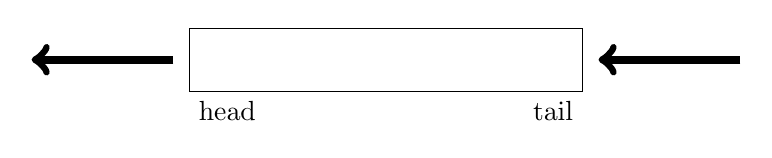
\begin{tikzpicture}

\draw (2.5, 0.4)
  node[draw, , , color=black,
       rounded corners=0cm, inner sep=0cm] {

\begin{minipage}[t][0.8cm]{5cm}
\mbox{}

\end{minipage}

};\draw[line width=0.1cm,black,->] (7,0.4) to  (5.2,0.4);
\draw[line width=0.1cm,black,->] (-0.2,0.4) to  (-2,0.4);

\node[anchor=north west] at (0,0)   {head};

\node[anchor=north east] at (5,0)   {tail};
\end{tikzpicture}

\end{center}


      
\li $T$ is \defone{balanced} if at each node,
every pair of children have heights differ by 0 or 1.
\end{myenum}

\begin{ex}
If $T$ is a balanced tree, does it mean that $T$ is complete?
If $T$ is complete, does it mean that $T$ is balanced?
\qed
\end{ex}

Let $T$ be a $k$--ary tree with height $h$ and the total 
number of nodes is $n$.
At level $\ell$,
there are at most $k^\ell$ nodes.
(Don't forget that the first level that contains only the root
is called level $0$.)
In particular for a binary tree, at level $\ell$, 
there are $2^\ell$ nodes.

Therefore if the height is $h$, $T$ can have at most
\[
k^0 + k^1 + \cdots + k^h = \frac{k^{h+1} - 1}{k-1}
\]
nodes.
(Remember your geometric sum formula?)
In particular, for a binary tree, $T$ can have at most
\[
2^{h+1} - 1
\]
nodes.
Since $T$ has $n$ nodes, we must have the following relation
between $n$ and $h$ for a $k$--ary tree:
\[
h + 1 \leq n \leq \frac{k^{h+1} - 1}{k-1}
\]
And for the case of binary tree, we have
\[
h + 1 \leq n \leq 2^{h+1}
\]

 % done
\newpage\sectionthree{Implementation}
\begin{python0}
from solutions import *; clear()
\end{python0}

Here's an abstract base class:
{\small
\begin{Verbatim}[frame=single]
class Hashable
{
public:
    virtual unsigned int hash(unsigned int) = 0;
};
\end{Verbatim}
}
This is just to impose a hash method on a subclass.
So for instance you can do this:
{\small
\begin{Verbatim}[frame=single]
class Name
{
public:
    Name(const std::string & s)
        : s_(s)
    {}

private:
    std::string s_;
};


class HashableName: public Name, Hashable
{
public:
    HashableName(const std::string & s)
        : Name(s) 
    {}
    
    unsigned int hash(unsigned int s)
    {
        unsigned int h = 0;
        ... compute h using s_ ...
        return h % s;
    }
};
\end{Verbatim}
}
Here's the class for a row of key-value in the hash table:
{\small
\begin{Verbatim}[frame=single]
template < typename Key, typename Value >
class KeyValue
{
private:
    Key key_;
    Value value_;
};
\end{Verbatim}
}
and here's the class for a row in the hash table together with a 
flag:
{\small
\begin{Verbatim}[frame=single]
template < typename Key, typename Value >
class HashtableRow
{
public:
    enum State
    { 
        AVAILABLE, NOT_AVAILABLE, DELETED 
    };
private:
    State state_;
    KeyValue< Key, Value > keyvalue_;
};
\end{Verbatim}
}
And now we have the hash table:
{\small
\begin{Verbatim}[frame=single]
template < typename Key, typename Value >
class Hashtable
{
private:
    unsigned int size_;
    HashtableRow< Key, Value > * p_;
};
\end{Verbatim}
}

Note that the \verb!HashtableRow! class can be nested in the \verb!Hashtable!
class.


\begin{ex} 
  \label{ex:some-decision1}
  \tinysidebar{\debug{exercises/{empty0/question.tex}}}
  \solutionlink{sol:some-decision1}
  \qed
\end{ex} 
\begin{python0}
from solutions import *
add(label="ex:some-decision1",
    srcfilename='exercises/some-decision1/answer.tex') 
\end{python0}




\begin{ex} 
  \label{ex:some-decision1}
  \tinysidebar{\debug{exercises/{empty0/question.tex}}}
  \solutionlink{sol:some-decision1}
  \qed
\end{ex} 
\begin{python0}
from solutions import *
add(label="ex:some-decision1",
    srcfilename='exercises/some-decision1/answer.tex') 
\end{python0}



\begin{ex} 
  \label{ex:some-decision1}
  \tinysidebar{\debug{exercises/{empty0/question.tex}}}
  \solutionlink{sol:some-decision1}
  \qed
\end{ex} 
\begin{python0}
from solutions import *
add(label="ex:some-decision1",
    srcfilename='exercises/some-decision1/answer.tex') 
\end{python0}





\newpage
 % done
\newpage\input{traversal.tex} % done
\newpage\sectionthree{Trees and arithmetic expressions}
\begin{python0}
from solutions import *; clear()
\end{python0}

Trees can be used to represent arithmetic expressions.
For instance look at this:

\begin{center}
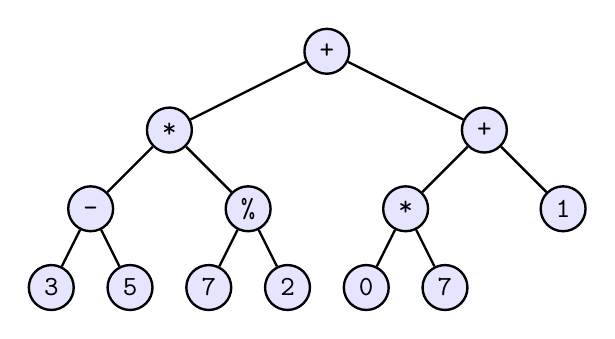
\begin{tikzpicture}

\fill[blue!10] (0.0, 0.0) circle (0.3);
\node [line width=0.03cm,black,minimum size=0.57cm,draw,circle] at (0.0,0.0)(+){};\draw (0.0, 0.0) node[color=black] {\texttt{+}};
\fill[blue!10] (-2.0, -1.0) circle (0.3);
\node [line width=0.03cm,black,minimum size=0.57cm,draw,circle] at (-2.0,-1.0)(*){};\draw (-2.0, -1.0) node[color=black] {\texttt{*}};
\fill[blue!10] (2.0, -1.0) circle (0.3);
\node [line width=0.03cm,black,minimum size=0.57cm,draw,circle] at (2.0,-1.0)(c){};\draw (2.0, -1.0) node[color=black] {\texttt{+}};
\fill[blue!10] (-3.0, -2.0) circle (0.3);
\node [line width=0.03cm,black,minimum size=0.57cm,draw,circle] at (-3.0,-2.0)(-){};\draw (-3.0, -2.0) node[color=black] {\texttt{-}};
\fill[blue!10] (-1.0, -2.0) circle (0.3);
\node [line width=0.03cm,black,minimum size=0.57cm,draw,circle] at (-1.0,-2.0)(e){};\draw (-1.0, -2.0) node[color=black] {\texttt{\%}};
\fill[blue!10] (1.0, -2.0) circle (0.3);
\node [line width=0.03cm,black,minimum size=0.57cm,draw,circle] at (1.0,-2.0)(f){};\draw (1.0, -2.0) node[color=black] {\texttt{*}};
\fill[blue!10] (3.0, -2.0) circle (0.3);
\node [line width=0.03cm,black,minimum size=0.57cm,draw,circle] at (3.0,-2.0)(1){};\draw (3.0, -2.0) node[color=black] {\texttt{1}};
\fill[blue!10] (-3.5, -3.0) circle (0.3);
\node [line width=0.03cm,black,minimum size=0.57cm,draw,circle] at (-3.5,-3.0)(3){};\draw (-3.5, -3.0) node[color=black] {\texttt{3}};
\fill[blue!10] (-2.5, -3.0) circle (0.3);
\node [line width=0.03cm,black,minimum size=0.57cm,draw,circle] at (-2.5,-3.0)(5){};\draw (-2.5, -3.0) node[color=black] {\texttt{5}};
\fill[blue!10] (-1.5, -3.0) circle (0.3);
\node [line width=0.03cm,black,minimum size=0.57cm,draw,circle] at (-1.5,-3.0)(z){};\draw (-1.5, -3.0) node[color=black] {\texttt{7}};
\fill[blue!10] (-0.5, -3.0) circle (0.3);
\node [line width=0.03cm,black,minimum size=0.57cm,draw,circle] at (-0.5,-3.0)(2){};\draw (-0.5, -3.0) node[color=black] {\texttt{2}};
\fill[blue!10] (0.5, -3.0) circle (0.3);
\node [line width=0.03cm,black,minimum size=0.57cm,draw,circle] at (0.5,-3.0)(0){};\draw (0.5, -3.0) node[color=black] {\texttt{0}};
\fill[blue!10] (1.5, -3.0) circle (0.3);
\node [line width=0.03cm,black,minimum size=0.57cm,draw,circle] at (1.5,-3.0)(7){};\draw (1.5, -3.0) node[color=black] {\texttt{7}};\draw[line width=0.03cm,black] (+) to  (*);
\draw[line width=0.03cm,black] (+) to  (c);
\draw[line width=0.03cm,black] (*) to  (-);
\draw[line width=0.03cm,black] (*) to  (e);
\draw[line width=0.03cm,black] (c) to  (f);
\draw[line width=0.03cm,black] (c) to  (1);
\draw[line width=0.03cm,black] (-) to  (3);
\draw[line width=0.03cm,black] (-) to  (5);
\draw[line width=0.03cm,black] (e) to  (z);
\draw[line width=0.03cm,black] (e) to  (2);
\draw[line width=0.03cm,black] (f) to  (0);
\draw[line width=0.03cm,black] (f) to  (7);
\end{tikzpicture}

\end{center}



The value obtained from \lq\lq evaluating'' the tree is this:
\[
\texttt{(((3 - 5) * (7 \% 2)) + ((0 * 7) + 1))}
\]

You can think of the tree as a device that can be used to describe
order of operations, or if you like, it's a device that can be 
used to play the role of parentheses.
So really, you have been doing trees since elementary school, right?

\begin{ex}
Assuming the above tree is a tree with node that contain characters,
Write a function to traverse the tree and produce the 
string
\[
\texttt{(((3 - 5) * (7 \% 2)) + ((0 * 7) + 1))}
\]
What tree traversal would you use?
\qed
\end{ex}
 % done
\newpage\sectionthree{Some basic operations}
\begin{python0}
from solutions import *; clear()
\end{python0}

Here are some basic methods on a node.
Note that there are so many different variations of trees
that some of the methods might not apply for some cases.
So you have to understand the context.

The following are some basic queries (they don't modify the 
tree in any way):

\begin{console}
node.is_root()           true iff node is a root
node.is_leaf()           true iff node is a leaf
node.is_nonleaf()        true iff node is non-leaf

node.level()             level of node
node.height()            height of node
node.depth()             depth of node
node.size()              number of descendents + 1
\end{console}

Note that for instance in the case of \texttt{is\_root()},
the only way for this to be meaningful is when the node
has a parent pointer: a node is a root is the parent pointer
is \texttt{NULL}.
So if your node class does not have a parent pointer
member, then this method is not meaningful.

For querying ancestor information, you have the following:
\begin{console}
node.parent()            pointer/reference to parent
node.root()              pointer/reference to root 
\end{console}

The next two methods are related to siblings of a node.
This is usually only available if the siblings are
organized in an iterable manner such as for instance
if the siblings form a linked list.
\begin{console}
node.next()              pointer/reference to next 
                         sibling; NULL if there is no 
                         next sibling.
node.prev()              pointer/reference to previous 
                         sibling; NULL if there is no
                         previous sibling.
\end{console}
In the case where the siblings form a circular list, 
it's of course important that you don't run into an infinite loop!

For querying children related information, you might have the
following:
\begin{console}
node.num_children()      number of children
node.children()          pointer/reference to iterable
                         container with children
node.first_child()       first child (assuming children 
                         are ordered)
node.last_child()        pointer/reference to last child 
                         (assuming children are ordered)
node.child(i)            pointer/reference to the i-th 
                         child
\end{console}
Sometimes the following descendent queries are useful too:
\begin{console}
node.leftmost()          pointer/reference to leftmost
                         starting at node; for a binary
                         tree, keep following the left
                         pointer/reference
node.rightmost()         pointer/reference to rightmost
                         starting at node; for a binary
                         tree, keep following the right
                         pointer/reference
\end{console}

For insertion, look at this binary tree:

\begin{center}
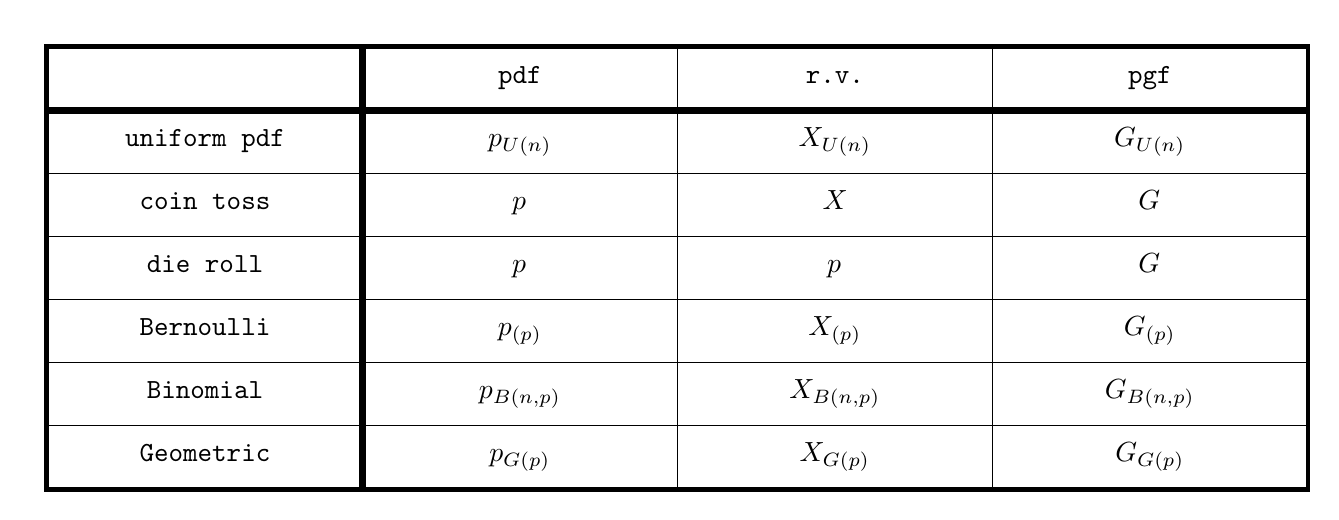
\begin{tikzpicture}

\draw (2.0, -0.4)
  node[draw, line width=0.02cm, , color=black,
       rounded corners=0cm, inner sep=0cm] {

\begin{minipage}[t][0.8cm]{4.0cm}
\mbox{}

\end{minipage}

};\draw (2.0, -0.4) node[color=black] {{\texttt{{\vphantom{pdfr.v.pgfuniform pdfcoin tossdie rollBernoulliBinomialGeometric$p_{U(n)}$$X_{U(n)}$$G_{U(n)}$$p_{\COIN}$$X_{\COIN}$$G_{\COIN}$$p_{\DIE}$$G_{\DIE}$$p_{\BERNOULLI(p)}$$X_{\BERNOULLI(p)}$$G_{\BERNOULLI(p)}$$p_{B(n,p)}$$X_{B(n,p)}$$G_{B(n,p)}$$p_{G(p)}$$X_{G(p)}$$G_{G(p)}$}}}}};\node[anchor=south] at (2.0,0.01) {};\node[anchor=east] at (-0.01,-0.4) {};
\draw (2.0, -0.4)
  node[draw, line width=0.06cm, , color=black,
       rounded corners=0cm, inner sep=0cm] {

\begin{minipage}[t][0.82cm]{4.02cm}
\mbox{}

\end{minipage}

};
\draw (6.0, -0.4)
  node[draw, line width=0.02cm, , color=black,
       rounded corners=0cm, inner sep=0cm] {

\begin{minipage}[t][0.8cm]{4.0cm}
\mbox{}

\end{minipage}

};\draw (6.0, -0.4) node[color=black] {{\texttt{{\vphantom{pdfr.v.pgfuniform pdfcoin tossdie rollBernoulliBinomialGeometric$p_{U(n)}$$X_{U(n)}$$G_{U(n)}$$p_{\COIN}$$X_{\COIN}$$G_{\COIN}$$p_{\DIE}$$G_{\DIE}$$p_{\BERNOULLI(p)}$$X_{\BERNOULLI(p)}$$G_{\BERNOULLI(p)}$$p_{B(n,p)}$$X_{B(n,p)}$$G_{B(n,p)}$$p_{G(p)}$$X_{G(p)}$$G_{G(p)}$}pdf}}}};
\draw (10.0, -0.4)
  node[draw, line width=0.02cm, , color=black,
       rounded corners=0cm, inner sep=0cm] {

\begin{minipage}[t][0.8cm]{4.0cm}
\mbox{}

\end{minipage}

};\draw (10.0, -0.4) node[color=black] {{\texttt{{\vphantom{pdfr.v.pgfuniform pdfcoin tossdie rollBernoulliBinomialGeometric$p_{U(n)}$$X_{U(n)}$$G_{U(n)}$$p_{\COIN}$$X_{\COIN}$$G_{\COIN}$$p_{\DIE}$$G_{\DIE}$$p_{\BERNOULLI(p)}$$X_{\BERNOULLI(p)}$$G_{\BERNOULLI(p)}$$p_{B(n,p)}$$X_{B(n,p)}$$G_{B(n,p)}$$p_{G(p)}$$X_{G(p)}$$G_{G(p)}$}r.v.}}}};
\draw (14.0, -0.4)
  node[draw, line width=0.02cm, , color=black,
       rounded corners=0cm, inner sep=0cm] {

\begin{minipage}[t][0.8cm]{4.0cm}
\mbox{}

\end{minipage}

};\draw (14.0, -0.4) node[color=black] {{\texttt{{\vphantom{pdfr.v.pgfuniform pdfcoin tossdie rollBernoulliBinomialGeometric$p_{U(n)}$$X_{U(n)}$$G_{U(n)}$$p_{\COIN}$$X_{\COIN}$$G_{\COIN}$$p_{\DIE}$$G_{\DIE}$$p_{\BERNOULLI(p)}$$X_{\BERNOULLI(p)}$$G_{\BERNOULLI(p)}$$p_{B(n,p)}$$X_{B(n,p)}$$G_{B(n,p)}$$p_{G(p)}$$X_{G(p)}$$G_{G(p)}$}pgf}}}};\node[anchor=south] at (6.0,0.01) {};\node[anchor=south] at (10.0,0.01) {};\node[anchor=south] at (14.0,0.01) {};\node[anchor=east] at (3.99,-0.4) {};
\draw (10.000000000000002, -0.4)
  node[draw, line width=0.06cm, , color=black,
       rounded corners=0cm, inner sep=0cm] {

\begin{minipage}[t][0.82cm]{12.02cm}
\mbox{}

\end{minipage}

};
\draw (2.0, -1.2000000000000002)
  node[draw, line width=0.02cm, , color=black,
       rounded corners=0cm, inner sep=0cm] {

\begin{minipage}[t][0.8cm]{4.0cm}
\mbox{}

\end{minipage}

};\draw (2.0, -1.2000000000000002) node[color=black] {{\texttt{{\vphantom{pdfr.v.pgfuniform pdfcoin tossdie rollBernoulliBinomialGeometric$p_{U(n)}$$X_{U(n)}$$G_{U(n)}$$p_{\COIN}$$X_{\COIN}$$G_{\COIN}$$p_{\DIE}$$G_{\DIE}$$p_{\BERNOULLI(p)}$$X_{\BERNOULLI(p)}$$G_{\BERNOULLI(p)}$$p_{B(n,p)}$$X_{B(n,p)}$$G_{B(n,p)}$$p_{G(p)}$$X_{G(p)}$$G_{G(p)}$}uniform pdf}}}};
\draw (2.0, -2.0)
  node[draw, line width=0.02cm, , color=black,
       rounded corners=0cm, inner sep=0cm] {

\begin{minipage}[t][0.8cm]{4.0cm}
\mbox{}

\end{minipage}

};\draw (2.0, -2.0) node[color=black] {{\texttt{{\vphantom{pdfr.v.pgfuniform pdfcoin tossdie rollBernoulliBinomialGeometric$p_{U(n)}$$X_{U(n)}$$G_{U(n)}$$p_{\COIN}$$X_{\COIN}$$G_{\COIN}$$p_{\DIE}$$G_{\DIE}$$p_{\BERNOULLI(p)}$$X_{\BERNOULLI(p)}$$G_{\BERNOULLI(p)}$$p_{B(n,p)}$$X_{B(n,p)}$$G_{B(n,p)}$$p_{G(p)}$$X_{G(p)}$$G_{G(p)}$}coin toss}}}};
\draw (2.0, -2.8000000000000003)
  node[draw, line width=0.02cm, , color=black,
       rounded corners=0cm, inner sep=0cm] {

\begin{minipage}[t][0.8cm]{4.0cm}
\mbox{}

\end{minipage}

};\draw (2.0, -2.8000000000000003) node[color=black] {{\texttt{{\vphantom{pdfr.v.pgfuniform pdfcoin tossdie rollBernoulliBinomialGeometric$p_{U(n)}$$X_{U(n)}$$G_{U(n)}$$p_{\COIN}$$X_{\COIN}$$G_{\COIN}$$p_{\DIE}$$G_{\DIE}$$p_{\BERNOULLI(p)}$$X_{\BERNOULLI(p)}$$G_{\BERNOULLI(p)}$$p_{B(n,p)}$$X_{B(n,p)}$$G_{B(n,p)}$$p_{G(p)}$$X_{G(p)}$$G_{G(p)}$}die roll}}}};
\draw (2.0, -3.6)
  node[draw, line width=0.02cm, , color=black,
       rounded corners=0cm, inner sep=0cm] {

\begin{minipage}[t][0.8cm]{4.0cm}
\mbox{}

\end{minipage}

};\draw (2.0, -3.6) node[color=black] {{\texttt{{\vphantom{pdfr.v.pgfuniform pdfcoin tossdie rollBernoulliBinomialGeometric$p_{U(n)}$$X_{U(n)}$$G_{U(n)}$$p_{\COIN}$$X_{\COIN}$$G_{\COIN}$$p_{\DIE}$$G_{\DIE}$$p_{\BERNOULLI(p)}$$X_{\BERNOULLI(p)}$$G_{\BERNOULLI(p)}$$p_{B(n,p)}$$X_{B(n,p)}$$G_{B(n,p)}$$p_{G(p)}$$X_{G(p)}$$G_{G(p)}$}Bernoulli}}}};
\draw (2.0, -4.4)
  node[draw, line width=0.02cm, , color=black,
       rounded corners=0cm, inner sep=0cm] {

\begin{minipage}[t][0.8cm]{4.0cm}
\mbox{}

\end{minipage}

};\draw (2.0, -4.4) node[color=black] {{\texttt{{\vphantom{pdfr.v.pgfuniform pdfcoin tossdie rollBernoulliBinomialGeometric$p_{U(n)}$$X_{U(n)}$$G_{U(n)}$$p_{\COIN}$$X_{\COIN}$$G_{\COIN}$$p_{\DIE}$$G_{\DIE}$$p_{\BERNOULLI(p)}$$X_{\BERNOULLI(p)}$$G_{\BERNOULLI(p)}$$p_{B(n,p)}$$X_{B(n,p)}$$G_{B(n,p)}$$p_{G(p)}$$X_{G(p)}$$G_{G(p)}$}Binomial}}}};
\draw (2.0, -5.199999999999999)
  node[draw, line width=0.02cm, , color=black,
       rounded corners=0cm, inner sep=0cm] {

\begin{minipage}[t][0.8cm]{4.0cm}
\mbox{}

\end{minipage}

};\draw (2.0, -5.199999999999999) node[color=black] {{\texttt{{\vphantom{pdfr.v.pgfuniform pdfcoin tossdie rollBernoulliBinomialGeometric$p_{U(n)}$$X_{U(n)}$$G_{U(n)}$$p_{\COIN}$$X_{\COIN}$$G_{\COIN}$$p_{\DIE}$$G_{\DIE}$$p_{\BERNOULLI(p)}$$X_{\BERNOULLI(p)}$$G_{\BERNOULLI(p)}$$p_{B(n,p)}$$X_{B(n,p)}$$G_{B(n,p)}$$p_{G(p)}$$X_{G(p)}$$G_{G(p)}$}Geometric}}}};\node[anchor=south] at (2.0,-0.79) {};\node[anchor=east] at (-0.01,-1.2000000000000002) {};\node[anchor=east] at (-0.01,-2.0000000000000004) {};\node[anchor=east] at (-0.01,-2.8000000000000003) {};\node[anchor=east] at (-0.01,-3.6) {};\node[anchor=east] at (-0.01,-4.4) {};\node[anchor=east] at (-0.01,-5.199999999999999) {};
\draw (2.0, -3.1999999999999997)
  node[draw, line width=0.06cm, , color=black,
       rounded corners=0cm, inner sep=0cm] {

\begin{minipage}[t][4.82cm]{4.02cm}
\mbox{}

\end{minipage}

};
\draw (6.0, -1.2000000000000002)
  node[draw, line width=0.02cm, , color=black,
       rounded corners=0cm, inner sep=0cm] {

\begin{minipage}[t][0.8cm]{4.0cm}
\mbox{}

\end{minipage}

};\draw (6.0, -1.2000000000000002) node[color=black] {{\texttt{{\vphantom{pdfr.v.pgfuniform pdfcoin tossdie rollBernoulliBinomialGeometric$p_{U(n)}$$X_{U(n)}$$G_{U(n)}$$p_{\COIN}$$X_{\COIN}$$G_{\COIN}$$p_{\DIE}$$G_{\DIE}$$p_{\BERNOULLI(p)}$$X_{\BERNOULLI(p)}$$G_{\BERNOULLI(p)}$$p_{B(n,p)}$$X_{B(n,p)}$$G_{B(n,p)}$$p_{G(p)}$$X_{G(p)}$$G_{G(p)}$}$p_{U(n)}$}}}};
\draw (10.0, -1.2000000000000002)
  node[draw, line width=0.02cm, , color=black,
       rounded corners=0cm, inner sep=0cm] {

\begin{minipage}[t][0.8cm]{4.0cm}
\mbox{}

\end{minipage}

};\draw (10.0, -1.2000000000000002) node[color=black] {{\texttt{{\vphantom{pdfr.v.pgfuniform pdfcoin tossdie rollBernoulliBinomialGeometric$p_{U(n)}$$X_{U(n)}$$G_{U(n)}$$p_{\COIN}$$X_{\COIN}$$G_{\COIN}$$p_{\DIE}$$G_{\DIE}$$p_{\BERNOULLI(p)}$$X_{\BERNOULLI(p)}$$G_{\BERNOULLI(p)}$$p_{B(n,p)}$$X_{B(n,p)}$$G_{B(n,p)}$$p_{G(p)}$$X_{G(p)}$$G_{G(p)}$}$X_{U(n)}$}}}};
\draw (14.0, -1.2000000000000002)
  node[draw, line width=0.02cm, , color=black,
       rounded corners=0cm, inner sep=0cm] {

\begin{minipage}[t][0.8cm]{4.0cm}
\mbox{}

\end{minipage}

};\draw (14.0, -1.2000000000000002) node[color=black] {{\texttt{{\vphantom{pdfr.v.pgfuniform pdfcoin tossdie rollBernoulliBinomialGeometric$p_{U(n)}$$X_{U(n)}$$G_{U(n)}$$p_{\COIN}$$X_{\COIN}$$G_{\COIN}$$p_{\DIE}$$G_{\DIE}$$p_{\BERNOULLI(p)}$$X_{\BERNOULLI(p)}$$G_{\BERNOULLI(p)}$$p_{B(n,p)}$$X_{B(n,p)}$$G_{B(n,p)}$$p_{G(p)}$$X_{G(p)}$$G_{G(p)}$}$G_{U(n)}$}}}};
\draw (6.0, -2.0)
  node[draw, line width=0.02cm, , color=black,
       rounded corners=0cm, inner sep=0cm] {

\begin{minipage}[t][0.8cm]{4.0cm}
\mbox{}

\end{minipage}

};\draw (6.0, -2.0) node[color=black] {{\texttt{{\vphantom{pdfr.v.pgfuniform pdfcoin tossdie rollBernoulliBinomialGeometric$p_{U(n)}$$X_{U(n)}$$G_{U(n)}$$p_{\COIN}$$X_{\COIN}$$G_{\COIN}$$p_{\DIE}$$G_{\DIE}$$p_{\BERNOULLI(p)}$$X_{\BERNOULLI(p)}$$G_{\BERNOULLI(p)}$$p_{B(n,p)}$$X_{B(n,p)}$$G_{B(n,p)}$$p_{G(p)}$$X_{G(p)}$$G_{G(p)}$}$p_{\COIN}$}}}};
\draw (10.0, -2.0)
  node[draw, line width=0.02cm, , color=black,
       rounded corners=0cm, inner sep=0cm] {

\begin{minipage}[t][0.8cm]{4.0cm}
\mbox{}

\end{minipage}

};\draw (10.0, -2.0) node[color=black] {{\texttt{{\vphantom{pdfr.v.pgfuniform pdfcoin tossdie rollBernoulliBinomialGeometric$p_{U(n)}$$X_{U(n)}$$G_{U(n)}$$p_{\COIN}$$X_{\COIN}$$G_{\COIN}$$p_{\DIE}$$G_{\DIE}$$p_{\BERNOULLI(p)}$$X_{\BERNOULLI(p)}$$G_{\BERNOULLI(p)}$$p_{B(n,p)}$$X_{B(n,p)}$$G_{B(n,p)}$$p_{G(p)}$$X_{G(p)}$$G_{G(p)}$}$X_{\COIN}$}}}};
\draw (14.0, -2.0)
  node[draw, line width=0.02cm, , color=black,
       rounded corners=0cm, inner sep=0cm] {

\begin{minipage}[t][0.8cm]{4.0cm}
\mbox{}

\end{minipage}

};\draw (14.0, -2.0) node[color=black] {{\texttt{{\vphantom{pdfr.v.pgfuniform pdfcoin tossdie rollBernoulliBinomialGeometric$p_{U(n)}$$X_{U(n)}$$G_{U(n)}$$p_{\COIN}$$X_{\COIN}$$G_{\COIN}$$p_{\DIE}$$G_{\DIE}$$p_{\BERNOULLI(p)}$$X_{\BERNOULLI(p)}$$G_{\BERNOULLI(p)}$$p_{B(n,p)}$$X_{B(n,p)}$$G_{B(n,p)}$$p_{G(p)}$$X_{G(p)}$$G_{G(p)}$}$G_{\COIN}$}}}};
\draw (6.0, -2.8000000000000003)
  node[draw, line width=0.02cm, , color=black,
       rounded corners=0cm, inner sep=0cm] {

\begin{minipage}[t][0.8cm]{4.0cm}
\mbox{}

\end{minipage}

};\draw (6.0, -2.8000000000000003) node[color=black] {{\texttt{{\vphantom{pdfr.v.pgfuniform pdfcoin tossdie rollBernoulliBinomialGeometric$p_{U(n)}$$X_{U(n)}$$G_{U(n)}$$p_{\COIN}$$X_{\COIN}$$G_{\COIN}$$p_{\DIE}$$G_{\DIE}$$p_{\BERNOULLI(p)}$$X_{\BERNOULLI(p)}$$G_{\BERNOULLI(p)}$$p_{B(n,p)}$$X_{B(n,p)}$$G_{B(n,p)}$$p_{G(p)}$$X_{G(p)}$$G_{G(p)}$}$p_{\DIE}$}}}};
\draw (10.0, -2.8000000000000003)
  node[draw, line width=0.02cm, , color=black,
       rounded corners=0cm, inner sep=0cm] {

\begin{minipage}[t][0.8cm]{4.0cm}
\mbox{}

\end{minipage}

};\draw (10.0, -2.8000000000000003) node[color=black] {{\texttt{{\vphantom{pdfr.v.pgfuniform pdfcoin tossdie rollBernoulliBinomialGeometric$p_{U(n)}$$X_{U(n)}$$G_{U(n)}$$p_{\COIN}$$X_{\COIN}$$G_{\COIN}$$p_{\DIE}$$G_{\DIE}$$p_{\BERNOULLI(p)}$$X_{\BERNOULLI(p)}$$G_{\BERNOULLI(p)}$$p_{B(n,p)}$$X_{B(n,p)}$$G_{B(n,p)}$$p_{G(p)}$$X_{G(p)}$$G_{G(p)}$}$p_{\DIE}$}}}};
\draw (14.0, -2.8000000000000003)
  node[draw, line width=0.02cm, , color=black,
       rounded corners=0cm, inner sep=0cm] {

\begin{minipage}[t][0.8cm]{4.0cm}
\mbox{}

\end{minipage}

};\draw (14.0, -2.8000000000000003) node[color=black] {{\texttt{{\vphantom{pdfr.v.pgfuniform pdfcoin tossdie rollBernoulliBinomialGeometric$p_{U(n)}$$X_{U(n)}$$G_{U(n)}$$p_{\COIN}$$X_{\COIN}$$G_{\COIN}$$p_{\DIE}$$G_{\DIE}$$p_{\BERNOULLI(p)}$$X_{\BERNOULLI(p)}$$G_{\BERNOULLI(p)}$$p_{B(n,p)}$$X_{B(n,p)}$$G_{B(n,p)}$$p_{G(p)}$$X_{G(p)}$$G_{G(p)}$}$G_{\DIE}$}}}};
\draw (6.0, -3.6)
  node[draw, line width=0.02cm, , color=black,
       rounded corners=0cm, inner sep=0cm] {

\begin{minipage}[t][0.8cm]{4.0cm}
\mbox{}

\end{minipage}

};\draw (6.0, -3.6) node[color=black] {{\texttt{{\vphantom{pdfr.v.pgfuniform pdfcoin tossdie rollBernoulliBinomialGeometric$p_{U(n)}$$X_{U(n)}$$G_{U(n)}$$p_{\COIN}$$X_{\COIN}$$G_{\COIN}$$p_{\DIE}$$G_{\DIE}$$p_{\BERNOULLI(p)}$$X_{\BERNOULLI(p)}$$G_{\BERNOULLI(p)}$$p_{B(n,p)}$$X_{B(n,p)}$$G_{B(n,p)}$$p_{G(p)}$$X_{G(p)}$$G_{G(p)}$}$p_{\BERNOULLI(p)}$}}}};
\draw (10.0, -3.6)
  node[draw, line width=0.02cm, , color=black,
       rounded corners=0cm, inner sep=0cm] {

\begin{minipage}[t][0.8cm]{4.0cm}
\mbox{}

\end{minipage}

};\draw (10.0, -3.6) node[color=black] {{\texttt{{\vphantom{pdfr.v.pgfuniform pdfcoin tossdie rollBernoulliBinomialGeometric$p_{U(n)}$$X_{U(n)}$$G_{U(n)}$$p_{\COIN}$$X_{\COIN}$$G_{\COIN}$$p_{\DIE}$$G_{\DIE}$$p_{\BERNOULLI(p)}$$X_{\BERNOULLI(p)}$$G_{\BERNOULLI(p)}$$p_{B(n,p)}$$X_{B(n,p)}$$G_{B(n,p)}$$p_{G(p)}$$X_{G(p)}$$G_{G(p)}$}$X_{\BERNOULLI(p)}$}}}};
\draw (14.0, -3.6)
  node[draw, line width=0.02cm, , color=black,
       rounded corners=0cm, inner sep=0cm] {

\begin{minipage}[t][0.8cm]{4.0cm}
\mbox{}

\end{minipage}

};\draw (14.0, -3.6) node[color=black] {{\texttt{{\vphantom{pdfr.v.pgfuniform pdfcoin tossdie rollBernoulliBinomialGeometric$p_{U(n)}$$X_{U(n)}$$G_{U(n)}$$p_{\COIN}$$X_{\COIN}$$G_{\COIN}$$p_{\DIE}$$G_{\DIE}$$p_{\BERNOULLI(p)}$$X_{\BERNOULLI(p)}$$G_{\BERNOULLI(p)}$$p_{B(n,p)}$$X_{B(n,p)}$$G_{B(n,p)}$$p_{G(p)}$$X_{G(p)}$$G_{G(p)}$}$G_{\BERNOULLI(p)}$}}}};
\draw (6.0, -4.4)
  node[draw, line width=0.02cm, , color=black,
       rounded corners=0cm, inner sep=0cm] {

\begin{minipage}[t][0.8cm]{4.0cm}
\mbox{}

\end{minipage}

};\draw (6.0, -4.4) node[color=black] {{\texttt{{\vphantom{pdfr.v.pgfuniform pdfcoin tossdie rollBernoulliBinomialGeometric$p_{U(n)}$$X_{U(n)}$$G_{U(n)}$$p_{\COIN}$$X_{\COIN}$$G_{\COIN}$$p_{\DIE}$$G_{\DIE}$$p_{\BERNOULLI(p)}$$X_{\BERNOULLI(p)}$$G_{\BERNOULLI(p)}$$p_{B(n,p)}$$X_{B(n,p)}$$G_{B(n,p)}$$p_{G(p)}$$X_{G(p)}$$G_{G(p)}$}$p_{B(n,p)}$}}}};
\draw (10.0, -4.4)
  node[draw, line width=0.02cm, , color=black,
       rounded corners=0cm, inner sep=0cm] {

\begin{minipage}[t][0.8cm]{4.0cm}
\mbox{}

\end{minipage}

};\draw (10.0, -4.4) node[color=black] {{\texttt{{\vphantom{pdfr.v.pgfuniform pdfcoin tossdie rollBernoulliBinomialGeometric$p_{U(n)}$$X_{U(n)}$$G_{U(n)}$$p_{\COIN}$$X_{\COIN}$$G_{\COIN}$$p_{\DIE}$$G_{\DIE}$$p_{\BERNOULLI(p)}$$X_{\BERNOULLI(p)}$$G_{\BERNOULLI(p)}$$p_{B(n,p)}$$X_{B(n,p)}$$G_{B(n,p)}$$p_{G(p)}$$X_{G(p)}$$G_{G(p)}$}$X_{B(n,p)}$}}}};
\draw (14.0, -4.4)
  node[draw, line width=0.02cm, , color=black,
       rounded corners=0cm, inner sep=0cm] {

\begin{minipage}[t][0.8cm]{4.0cm}
\mbox{}

\end{minipage}

};\draw (14.0, -4.4) node[color=black] {{\texttt{{\vphantom{pdfr.v.pgfuniform pdfcoin tossdie rollBernoulliBinomialGeometric$p_{U(n)}$$X_{U(n)}$$G_{U(n)}$$p_{\COIN}$$X_{\COIN}$$G_{\COIN}$$p_{\DIE}$$G_{\DIE}$$p_{\BERNOULLI(p)}$$X_{\BERNOULLI(p)}$$G_{\BERNOULLI(p)}$$p_{B(n,p)}$$X_{B(n,p)}$$G_{B(n,p)}$$p_{G(p)}$$X_{G(p)}$$G_{G(p)}$}$G_{B(n,p)}$}}}};
\draw (6.0, -5.199999999999999)
  node[draw, line width=0.02cm, , color=black,
       rounded corners=0cm, inner sep=0cm] {

\begin{minipage}[t][0.8cm]{4.0cm}
\mbox{}

\end{minipage}

};\draw (6.0, -5.199999999999999) node[color=black] {{\texttt{{\vphantom{pdfr.v.pgfuniform pdfcoin tossdie rollBernoulliBinomialGeometric$p_{U(n)}$$X_{U(n)}$$G_{U(n)}$$p_{\COIN}$$X_{\COIN}$$G_{\COIN}$$p_{\DIE}$$G_{\DIE}$$p_{\BERNOULLI(p)}$$X_{\BERNOULLI(p)}$$G_{\BERNOULLI(p)}$$p_{B(n,p)}$$X_{B(n,p)}$$G_{B(n,p)}$$p_{G(p)}$$X_{G(p)}$$G_{G(p)}$}$p_{G(p)}$}}}};
\draw (10.0, -5.199999999999999)
  node[draw, line width=0.02cm, , color=black,
       rounded corners=0cm, inner sep=0cm] {

\begin{minipage}[t][0.8cm]{4.0cm}
\mbox{}

\end{minipage}

};\draw (10.0, -5.199999999999999) node[color=black] {{\texttt{{\vphantom{pdfr.v.pgfuniform pdfcoin tossdie rollBernoulliBinomialGeometric$p_{U(n)}$$X_{U(n)}$$G_{U(n)}$$p_{\COIN}$$X_{\COIN}$$G_{\COIN}$$p_{\DIE}$$G_{\DIE}$$p_{\BERNOULLI(p)}$$X_{\BERNOULLI(p)}$$G_{\BERNOULLI(p)}$$p_{B(n,p)}$$X_{B(n,p)}$$G_{B(n,p)}$$p_{G(p)}$$X_{G(p)}$$G_{G(p)}$}$X_{G(p)}$}}}};
\draw (14.0, -5.199999999999999)
  node[draw, line width=0.02cm, , color=black,
       rounded corners=0cm, inner sep=0cm] {

\begin{minipage}[t][0.8cm]{4.0cm}
\mbox{}

\end{minipage}

};\draw (14.0, -5.199999999999999) node[color=black] {{\texttt{{\vphantom{pdfr.v.pgfuniform pdfcoin tossdie rollBernoulliBinomialGeometric$p_{U(n)}$$X_{U(n)}$$G_{U(n)}$$p_{\COIN}$$X_{\COIN}$$G_{\COIN}$$p_{\DIE}$$G_{\DIE}$$p_{\BERNOULLI(p)}$$X_{\BERNOULLI(p)}$$G_{\BERNOULLI(p)}$$p_{B(n,p)}$$X_{B(n,p)}$$G_{B(n,p)}$$p_{G(p)}$$X_{G(p)}$$G_{G(p)}$}$G_{G(p)}$}}}};\node[anchor=south] at (6.0,-0.79) {};\node[anchor=south] at (10.0,-0.79) {};\node[anchor=south] at (14.0,-0.79) {};\node[anchor=east] at (3.99,-1.2000000000000002) {};\node[anchor=east] at (3.99,-2.0000000000000004) {};\node[anchor=east] at (3.99,-2.8000000000000003) {};\node[anchor=east] at (3.99,-3.6) {};\node[anchor=east] at (3.99,-4.4) {};\node[anchor=east] at (3.99,-5.199999999999999) {};
\draw (10.000000000000002, -3.1999999999999997)
  node[draw, line width=0.06cm, , color=black,
       rounded corners=0cm, inner sep=0cm] {

\begin{minipage}[t][4.82cm]{12.02cm}
\mbox{}

\end{minipage}

};
\end{tikzpicture}

\end{center}



The most common case of insertion is as a child at a position that
is available.
For instance in the above, note that at node $l$ 
you can insert a node at the left or the right.
However note that at $h$, you can only insert at the left.
Note that the above also makes sense when the node that is
inserted is actually the root of a tree.
In the case of a $k$--ary tree, 
if child-$i$ is available, you can insert a node at that 
position.

Most tree API do not include inserting a node at a place that is not available.
Although that's entirely reasonable.
For instance there's no reason why you cannot do an insertion
right at the node $d$ with new data $o$ (i.e., it goes
between $d$ and $j$):

\begin{center}
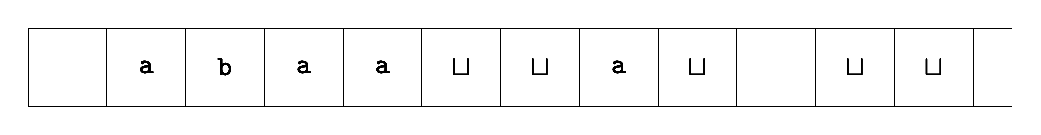
\begin{tikzpicture}

\draw (0.49999999999999994, 0.49999999999999994)
  node[draw, line width=0.01cm, , color=black,
       rounded corners=0cm, inner sep=0cm] {

\begin{minipage}[t][1.0cm]{1.0cm}
\mbox{}

\end{minipage}

};\draw (0.49999999999999994, 0.49999999999999994) node[color=black] {\texttt{\DOLLAR}};
\draw (1.5, 0.49999999999999994)
  node[draw, line width=0.01cm, , color=black,
       rounded corners=0cm, inner sep=0cm] {

\begin{minipage}[t][1.0cm]{1.0cm}
\mbox{}

\end{minipage}

};\draw (1.5, 0.49999999999999994) node[color=black] {\texttt{a}};
\draw (2.5, 0.49999999999999994)
  node[draw, line width=0.01cm, , color=black,
       rounded corners=0cm, inner sep=0cm] {

\begin{minipage}[t][1.0cm]{1.0cm}
\mbox{}

\end{minipage}

};\draw (2.5, 0.49999999999999994) node[color=black] {\texttt{b}};
\draw (3.5, 0.49999999999999994)
  node[draw, line width=0.01cm, , color=black,
       rounded corners=0cm, inner sep=0cm] {

\begin{minipage}[t][1.0cm]{1.0cm}
\mbox{}

\end{minipage}

};\draw (3.5, 0.49999999999999994) node[color=black] {\texttt{a}};
\draw (4.5, 0.49999999999999994)
  node[draw, line width=0.01cm, , color=black,
       rounded corners=0cm, inner sep=0cm] {

\begin{minipage}[t][1.0cm]{1.0cm}
\mbox{}

\end{minipage}

};\draw (4.5, 0.49999999999999994) node[color=black] {\texttt{a}};
\draw (5.5, 0.49999999999999994)
  node[draw, line width=0.01cm, , color=black,
       rounded corners=0cm, inner sep=0cm] {

\begin{minipage}[t][1.0cm]{1.0cm}
\mbox{}

\end{minipage}

};\draw (5.5, 0.49999999999999994) node[color=black] {\texttt{$\sqcup$}};
\draw (6.5, 0.49999999999999994)
  node[draw, line width=0.01cm, , color=black,
       rounded corners=0cm, inner sep=0cm] {

\begin{minipage}[t][1.0cm]{1.0cm}
\mbox{}

\end{minipage}

};\draw (6.5, 0.49999999999999994) node[color=black] {\texttt{$\sqcup$}};
\draw (7.5, 0.49999999999999994)
  node[draw, line width=0.01cm, , color=black,
       rounded corners=0cm, inner sep=0cm] {

\begin{minipage}[t][1.0cm]{1.0cm}
\mbox{}

\end{minipage}

};\draw (7.5, 0.49999999999999994) node[color=black] {\texttt{a}};
\draw (8.5, 0.49999999999999994)
  node[draw, line width=0.01cm, , color=black,
       rounded corners=0cm, inner sep=0cm] {

\begin{minipage}[t][1.0cm]{1.0cm}
\mbox{}

\end{minipage}

};\draw (8.5, 0.49999999999999994) node[color=black] {\texttt{$\sqcup$}};
\draw (9.5, 0.49999999999999994)
  node[draw, line width=0.01cm, , color=black,
       rounded corners=0cm, inner sep=0cm] {

\begin{minipage}[t][1.0cm]{1.0cm}
\mbox{}

\end{minipage}

};\draw (9.5, 0.49999999999999994) node[color=black] {\texttt{$\EOT$}};
\draw (10.5, 0.49999999999999994)
  node[draw, line width=0.01cm, , color=black,
       rounded corners=0cm, inner sep=0cm] {

\begin{minipage}[t][1.0cm]{1.0cm}
\mbox{}

\end{minipage}

};\draw (10.5, 0.49999999999999994) node[color=black] {\texttt{$\sqcup$}};
\draw (11.5, 0.49999999999999994)
  node[draw, line width=0.01cm, , color=black,
       rounded corners=0cm, inner sep=0cm] {

\begin{minipage}[t][1.0cm]{1.0cm}
\mbox{}

\end{minipage}

};\draw (11.5, 0.49999999999999994) node[color=black] {\texttt{$\sqcup$}};
\draw (0.49999999999999994, 0.49999999999999994)
  node[draw, line width=0.01cm, , color=black,
       rounded corners=0cm, inner sep=0cm] {

\begin{minipage}[t][1.0cm]{1.0cm}
\mbox{}

\end{minipage}

};\draw (0.49999999999999994, 0.49999999999999994) node[color=black] {\texttt{\DOLLAR}};
\draw (1.5, 0.49999999999999994)
  node[draw, line width=0.01cm, , color=black,
       rounded corners=0cm, inner sep=0cm] {

\begin{minipage}[t][1.0cm]{1.0cm}
\mbox{}

\end{minipage}

};\draw (1.5, 0.49999999999999994) node[color=black] {\texttt{a}};
\draw (2.5, 0.49999999999999994)
  node[draw, line width=0.01cm, , color=black,
       rounded corners=0cm, inner sep=0cm] {

\begin{minipage}[t][1.0cm]{1.0cm}
\mbox{}

\end{minipage}

};\draw (2.5, 0.49999999999999994) node[color=black] {\texttt{b}};
\draw (3.5, 0.49999999999999994)
  node[draw, line width=0.01cm, , color=black,
       rounded corners=0cm, inner sep=0cm] {

\begin{minipage}[t][1.0cm]{1.0cm}
\mbox{}

\end{minipage}

};\draw (3.5, 0.49999999999999994) node[color=black] {\texttt{a}};
\draw (4.5, 0.49999999999999994)
  node[draw, line width=0.01cm, , color=black,
       rounded corners=0cm, inner sep=0cm] {

\begin{minipage}[t][1.0cm]{1.0cm}
\mbox{}

\end{minipage}

};\draw (4.5, 0.49999999999999994) node[color=black] {\texttt{a}};
\draw (5.5, 0.49999999999999994)
  node[draw, line width=0.01cm, , color=black,
       rounded corners=0cm, inner sep=0cm] {

\begin{minipage}[t][1.0cm]{1.0cm}
\mbox{}

\end{minipage}

};\draw (5.5, 0.49999999999999994) node[color=black] {\texttt{$\sqcup$}};
\draw (6.5, 0.49999999999999994)
  node[draw, line width=0.01cm, , color=black,
       rounded corners=0cm, inner sep=0cm] {

\begin{minipage}[t][1.0cm]{1.0cm}
\mbox{}

\end{minipage}

};\draw (6.5, 0.49999999999999994) node[color=black] {\texttt{$\sqcup$}};
\draw (7.5, 0.49999999999999994)
  node[draw, line width=0.01cm, , color=black,
       rounded corners=0cm, inner sep=0cm] {

\begin{minipage}[t][1.0cm]{1.0cm}
\mbox{}

\end{minipage}

};\draw (7.5, 0.49999999999999994) node[color=black] {\texttt{a}};
\draw (8.5, 0.49999999999999994)
  node[draw, line width=0.01cm, , color=black,
       rounded corners=0cm, inner sep=0cm] {

\begin{minipage}[t][1.0cm]{1.0cm}
\mbox{}

\end{minipage}

};\draw (8.5, 0.49999999999999994) node[color=black] {\texttt{$\sqcup$}};
\draw (9.5, 0.49999999999999994)
  node[draw, line width=0.01cm, , color=black,
       rounded corners=0cm, inner sep=0cm] {

\begin{minipage}[t][1.0cm]{1.0cm}
\mbox{}

\end{minipage}

};\draw (9.5, 0.49999999999999994) node[color=black] {\texttt{$\EOT$}};
\draw (10.5, 0.49999999999999994)
  node[draw, line width=0.01cm, , color=black,
       rounded corners=0cm, inner sep=0cm] {

\begin{minipage}[t][1.0cm]{1.0cm}
\mbox{}

\end{minipage}

};\draw (10.5, 0.49999999999999994) node[color=black] {\texttt{$\sqcup$}};
\draw (11.5, 0.49999999999999994)
  node[draw, line width=0.01cm, , color=black,
       rounded corners=0cm, inner sep=0cm] {

\begin{minipage}[t][1.0cm]{1.0cm}
\mbox{}

\end{minipage}

};\draw (11.5, 0.49999999999999994) node[color=black] {\texttt{$\sqcup$}};
\draw (0.49999999999999994, 0.49999999999999994)
  node[draw, line width=0.01cm, , color=black,
       rounded corners=0cm, inner sep=0cm] {

\begin{minipage}[t][1.0cm]{1.0cm}
\mbox{}

\end{minipage}

};\draw (0.49999999999999994, 0.49999999999999994) node[color=black] {\texttt{\DOLLAR}};
\draw (1.5, 0.49999999999999994)
  node[draw, line width=0.01cm, , color=black,
       rounded corners=0cm, inner sep=0cm] {

\begin{minipage}[t][1.0cm]{1.0cm}
\mbox{}

\end{minipage}

};\draw (1.5, 0.49999999999999994) node[color=black] {\texttt{a}};
\draw (2.5, 0.49999999999999994)
  node[draw, line width=0.01cm, , color=black,
       rounded corners=0cm, inner sep=0cm] {

\begin{minipage}[t][1.0cm]{1.0cm}
\mbox{}

\end{minipage}

};\draw (2.5, 0.49999999999999994) node[color=black] {\texttt{b}};
\draw (3.5, 0.49999999999999994)
  node[draw, line width=0.01cm, , color=black,
       rounded corners=0cm, inner sep=0cm] {

\begin{minipage}[t][1.0cm]{1.0cm}
\mbox{}

\end{minipage}

};\draw (3.5, 0.49999999999999994) node[color=black] {\texttt{a}};
\draw (4.5, 0.49999999999999994)
  node[draw, line width=0.01cm, , color=black,
       rounded corners=0cm, inner sep=0cm] {

\begin{minipage}[t][1.0cm]{1.0cm}
\mbox{}

\end{minipage}

};\draw (4.5, 0.49999999999999994) node[color=black] {\texttt{a}};
\draw (5.5, 0.49999999999999994)
  node[draw, line width=0.01cm, , color=black,
       rounded corners=0cm, inner sep=0cm] {

\begin{minipage}[t][1.0cm]{1.0cm}
\mbox{}

\end{minipage}

};\draw (5.5, 0.49999999999999994) node[color=black] {\texttt{$\sqcup$}};
\draw (6.5, 0.49999999999999994)
  node[draw, line width=0.01cm, , color=black,
       rounded corners=0cm, inner sep=0cm] {

\begin{minipage}[t][1.0cm]{1.0cm}
\mbox{}

\end{minipage}

};\draw (6.5, 0.49999999999999994) node[color=black] {\texttt{$\sqcup$}};
\draw (7.5, 0.49999999999999994)
  node[draw, line width=0.01cm, , color=black,
       rounded corners=0cm, inner sep=0cm] {

\begin{minipage}[t][1.0cm]{1.0cm}
\mbox{}

\end{minipage}

};\draw (7.5, 0.49999999999999994) node[color=black] {\texttt{a}};
\draw (8.5, 0.49999999999999994)
  node[draw, line width=0.01cm, , color=black,
       rounded corners=0cm, inner sep=0cm] {

\begin{minipage}[t][1.0cm]{1.0cm}
\mbox{}

\end{minipage}

};\draw (8.5, 0.49999999999999994) node[color=black] {\texttt{$\sqcup$}};
\draw (9.5, 0.49999999999999994)
  node[draw, line width=0.01cm, , color=black,
       rounded corners=0cm, inner sep=0cm] {

\begin{minipage}[t][1.0cm]{1.0cm}
\mbox{}

\end{minipage}

};\draw (9.5, 0.49999999999999994) node[color=black] {\texttt{$\EOT$}};
\draw (10.5, 0.49999999999999994)
  node[draw, line width=0.01cm, , color=black,
       rounded corners=0cm, inner sep=0cm] {

\begin{minipage}[t][1.0cm]{1.0cm}
\mbox{}

\end{minipage}

};\draw (10.5, 0.49999999999999994) node[color=black] {\texttt{$\sqcup$}};
\draw (11.5, 0.49999999999999994)
  node[draw, line width=0.01cm, , color=black,
       rounded corners=0cm, inner sep=0cm] {

\begin{minipage}[t][1.0cm]{1.0cm}
\mbox{}

\end{minipage}

};\draw (11.5, 0.49999999999999994) node[color=black] {\texttt{$\sqcup$}};
\draw (0.49999999999999994, 0.49999999999999994)
  node[draw, line width=0.01cm, , color=black,
       rounded corners=0cm, inner sep=0cm] {

\begin{minipage}[t][1.0cm]{1.0cm}
\mbox{}

\end{minipage}

};\draw (0.49999999999999994, 0.49999999999999994) node[color=black] {\texttt{\DOLLAR}};
\draw (1.5, 0.49999999999999994)
  node[draw, line width=0.01cm, , color=black,
       rounded corners=0cm, inner sep=0cm] {

\begin{minipage}[t][1.0cm]{1.0cm}
\mbox{}

\end{minipage}

};\draw (1.5, 0.49999999999999994) node[color=black] {\texttt{a}};
\draw (2.5, 0.49999999999999994)
  node[draw, line width=0.01cm, , color=black,
       rounded corners=0cm, inner sep=0cm] {

\begin{minipage}[t][1.0cm]{1.0cm}
\mbox{}

\end{minipage}

};\draw (2.5, 0.49999999999999994) node[color=black] {\texttt{b}};
\draw (3.5, 0.49999999999999994)
  node[draw, line width=0.01cm, , color=black,
       rounded corners=0cm, inner sep=0cm] {

\begin{minipage}[t][1.0cm]{1.0cm}
\mbox{}

\end{minipage}

};\draw (3.5, 0.49999999999999994) node[color=black] {\texttt{a}};
\draw (4.5, 0.49999999999999994)
  node[draw, line width=0.01cm, , color=black,
       rounded corners=0cm, inner sep=0cm] {

\begin{minipage}[t][1.0cm]{1.0cm}
\mbox{}

\end{minipage}

};\draw (4.5, 0.49999999999999994) node[color=black] {\texttt{a}};
\draw (5.5, 0.49999999999999994)
  node[draw, line width=0.01cm, , color=black,
       rounded corners=0cm, inner sep=0cm] {

\begin{minipage}[t][1.0cm]{1.0cm}
\mbox{}

\end{minipage}

};\draw (5.5, 0.49999999999999994) node[color=black] {\texttt{$\sqcup$}};
\draw (6.5, 0.49999999999999994)
  node[draw, line width=0.01cm, , color=black,
       rounded corners=0cm, inner sep=0cm] {

\begin{minipage}[t][1.0cm]{1.0cm}
\mbox{}

\end{minipage}

};\draw (6.5, 0.49999999999999994) node[color=black] {\texttt{$\sqcup$}};
\draw (7.5, 0.49999999999999994)
  node[draw, line width=0.01cm, , color=black,
       rounded corners=0cm, inner sep=0cm] {

\begin{minipage}[t][1.0cm]{1.0cm}
\mbox{}

\end{minipage}

};\draw (7.5, 0.49999999999999994) node[color=black] {\texttt{a}};
\draw (8.5, 0.49999999999999994)
  node[draw, line width=0.01cm, , color=black,
       rounded corners=0cm, inner sep=0cm] {

\begin{minipage}[t][1.0cm]{1.0cm}
\mbox{}

\end{minipage}

};\draw (8.5, 0.49999999999999994) node[color=black] {\texttt{$\sqcup$}};
\draw (9.5, 0.49999999999999994)
  node[draw, line width=0.01cm, , color=black,
       rounded corners=0cm, inner sep=0cm] {

\begin{minipage}[t][1.0cm]{1.0cm}
\mbox{}

\end{minipage}

};\draw (9.5, 0.49999999999999994) node[color=black] {\texttt{$\EOT$}};
\draw (10.5, 0.49999999999999994)
  node[draw, line width=0.01cm, , color=black,
       rounded corners=0cm, inner sep=0cm] {

\begin{minipage}[t][1.0cm]{1.0cm}
\mbox{}

\end{minipage}

};\draw (10.5, 0.49999999999999994) node[color=black] {\texttt{$\sqcup$}};
\draw (11.5, 0.49999999999999994)
  node[draw, line width=0.01cm, , color=black,
       rounded corners=0cm, inner sep=0cm] {

\begin{minipage}[t][1.0cm]{1.0cm}
\mbox{}

\end{minipage}

};\draw (11.5, 0.49999999999999994) node[color=black] {\texttt{$\sqcup$}};
\draw (0.49999999999999994, 0.49999999999999994)
  node[draw, line width=0.01cm, , color=black,
       rounded corners=0cm, inner sep=0cm] {

\begin{minipage}[t][1.0cm]{1.0cm}
\mbox{}

\end{minipage}

};\draw (0.49999999999999994, 0.49999999999999994) node[color=black] {\texttt{\DOLLAR}};
\draw (1.5, 0.49999999999999994)
  node[draw, line width=0.01cm, , color=black,
       rounded corners=0cm, inner sep=0cm] {

\begin{minipage}[t][1.0cm]{1.0cm}
\mbox{}

\end{minipage}

};\draw (1.5, 0.49999999999999994) node[color=black] {\texttt{a}};
\draw (2.5, 0.49999999999999994)
  node[draw, line width=0.01cm, , color=black,
       rounded corners=0cm, inner sep=0cm] {

\begin{minipage}[t][1.0cm]{1.0cm}
\mbox{}

\end{minipage}

};\draw (2.5, 0.49999999999999994) node[color=black] {\texttt{b}};
\draw (3.5, 0.49999999999999994)
  node[draw, line width=0.01cm, , color=black,
       rounded corners=0cm, inner sep=0cm] {

\begin{minipage}[t][1.0cm]{1.0cm}
\mbox{}

\end{minipage}

};\draw (3.5, 0.49999999999999994) node[color=black] {\texttt{a}};
\draw (4.5, 0.49999999999999994)
  node[draw, line width=0.01cm, , color=black,
       rounded corners=0cm, inner sep=0cm] {

\begin{minipage}[t][1.0cm]{1.0cm}
\mbox{}

\end{minipage}

};\draw (4.5, 0.49999999999999994) node[color=black] {\texttt{a}};
\draw (5.5, 0.49999999999999994)
  node[draw, line width=0.01cm, , color=black,
       rounded corners=0cm, inner sep=0cm] {

\begin{minipage}[t][1.0cm]{1.0cm}
\mbox{}

\end{minipage}

};\draw (5.5, 0.49999999999999994) node[color=black] {\texttt{$\sqcup$}};
\draw (6.5, 0.49999999999999994)
  node[draw, line width=0.01cm, , color=black,
       rounded corners=0cm, inner sep=0cm] {

\begin{minipage}[t][1.0cm]{1.0cm}
\mbox{}

\end{minipage}

};\draw (6.5, 0.49999999999999994) node[color=black] {\texttt{$\sqcup$}};
\draw (7.5, 0.49999999999999994)
  node[draw, line width=0.01cm, , color=black,
       rounded corners=0cm, inner sep=0cm] {

\begin{minipage}[t][1.0cm]{1.0cm}
\mbox{}

\end{minipage}

};\draw (7.5, 0.49999999999999994) node[color=black] {\texttt{a}};
\draw (8.5, 0.49999999999999994)
  node[draw, line width=0.01cm, , color=black,
       rounded corners=0cm, inner sep=0cm] {

\begin{minipage}[t][1.0cm]{1.0cm}
\mbox{}

\end{minipage}

};\draw (8.5, 0.49999999999999994) node[color=black] {\texttt{$\sqcup$}};
\draw (9.5, 0.49999999999999994)
  node[draw, line width=0.01cm, , color=black,
       rounded corners=0cm, inner sep=0cm] {

\begin{minipage}[t][1.0cm]{1.0cm}
\mbox{}

\end{minipage}

};\draw (9.5, 0.49999999999999994) node[color=black] {\texttt{$\EOT$}};
\draw (10.5, 0.49999999999999994)
  node[draw, line width=0.01cm, , color=black,
       rounded corners=0cm, inner sep=0cm] {

\begin{minipage}[t][1.0cm]{1.0cm}
\mbox{}

\end{minipage}

};\draw (10.5, 0.49999999999999994) node[color=black] {\texttt{$\sqcup$}};
\draw (11.5, 0.49999999999999994)
  node[draw, line width=0.01cm, , color=black,
       rounded corners=0cm, inner sep=0cm] {

\begin{minipage}[t][1.0cm]{1.0cm}
\mbox{}

\end{minipage}

};\draw (11.5, 0.49999999999999994) node[color=black] {\texttt{$\sqcup$}};
\draw (0.49999999999999994, 0.49999999999999994)
  node[draw, line width=0.01cm, , color=black,
       rounded corners=0cm, inner sep=0cm] {

\begin{minipage}[t][1.0cm]{1.0cm}
\mbox{}

\end{minipage}

};\draw (0.49999999999999994, 0.49999999999999994) node[color=black] {\texttt{\DOLLAR}};
\draw (1.5, 0.49999999999999994)
  node[draw, line width=0.01cm, , color=black,
       rounded corners=0cm, inner sep=0cm] {

\begin{minipage}[t][1.0cm]{1.0cm}
\mbox{}

\end{minipage}

};\draw (1.5, 0.49999999999999994) node[color=black] {\texttt{a}};
\draw (2.5, 0.49999999999999994)
  node[draw, line width=0.01cm, , color=black,
       rounded corners=0cm, inner sep=0cm] {

\begin{minipage}[t][1.0cm]{1.0cm}
\mbox{}

\end{minipage}

};\draw (2.5, 0.49999999999999994) node[color=black] {\texttt{b}};
\draw (3.5, 0.49999999999999994)
  node[draw, line width=0.01cm, , color=black,
       rounded corners=0cm, inner sep=0cm] {

\begin{minipage}[t][1.0cm]{1.0cm}
\mbox{}

\end{minipage}

};\draw (3.5, 0.49999999999999994) node[color=black] {\texttt{a}};
\draw (4.5, 0.49999999999999994)
  node[draw, line width=0.01cm, , color=black,
       rounded corners=0cm, inner sep=0cm] {

\begin{minipage}[t][1.0cm]{1.0cm}
\mbox{}

\end{minipage}

};\draw (4.5, 0.49999999999999994) node[color=black] {\texttt{a}};
\draw (5.5, 0.49999999999999994)
  node[draw, line width=0.01cm, , color=black,
       rounded corners=0cm, inner sep=0cm] {

\begin{minipage}[t][1.0cm]{1.0cm}
\mbox{}

\end{minipage}

};\draw (5.5, 0.49999999999999994) node[color=black] {\texttt{$\sqcup$}};
\draw (6.5, 0.49999999999999994)
  node[draw, line width=0.01cm, , color=black,
       rounded corners=0cm, inner sep=0cm] {

\begin{minipage}[t][1.0cm]{1.0cm}
\mbox{}

\end{minipage}

};\draw (6.5, 0.49999999999999994) node[color=black] {\texttt{$\sqcup$}};
\draw (7.5, 0.49999999999999994)
  node[draw, line width=0.01cm, , color=black,
       rounded corners=0cm, inner sep=0cm] {

\begin{minipage}[t][1.0cm]{1.0cm}
\mbox{}

\end{minipage}

};\draw (7.5, 0.49999999999999994) node[color=black] {\texttt{a}};
\draw (8.5, 0.49999999999999994)
  node[draw, line width=0.01cm, , color=black,
       rounded corners=0cm, inner sep=0cm] {

\begin{minipage}[t][1.0cm]{1.0cm}
\mbox{}

\end{minipage}

};\draw (8.5, 0.49999999999999994) node[color=black] {\texttt{$\sqcup$}};
\draw (9.5, 0.49999999999999994)
  node[draw, line width=0.01cm, , color=black,
       rounded corners=0cm, inner sep=0cm] {

\begin{minipage}[t][1.0cm]{1.0cm}
\mbox{}

\end{minipage}

};\draw (9.5, 0.49999999999999994) node[color=black] {\texttt{$\EOT$}};
\draw (10.5, 0.49999999999999994)
  node[draw, line width=0.01cm, , color=black,
       rounded corners=0cm, inner sep=0cm] {

\begin{minipage}[t][1.0cm]{1.0cm}
\mbox{}

\end{minipage}

};\draw (10.5, 0.49999999999999994) node[color=black] {\texttt{$\sqcup$}};
\draw (11.5, 0.49999999999999994)
  node[draw, line width=0.01cm, , color=black,
       rounded corners=0cm, inner sep=0cm] {

\begin{minipage}[t][1.0cm]{1.0cm}
\mbox{}

\end{minipage}

};\draw (11.5, 0.49999999999999994) node[color=black] {\texttt{$\sqcup$}};
\draw (0.49999999999999994, 0.49999999999999994)
  node[draw, line width=0.01cm, , color=black,
       rounded corners=0cm, inner sep=0cm] {

\begin{minipage}[t][1.0cm]{1.0cm}
\mbox{}

\end{minipage}

};\draw (0.49999999999999994, 0.49999999999999994) node[color=black] {\texttt{\DOLLAR}};
\draw (1.5, 0.49999999999999994)
  node[draw, line width=0.01cm, , color=black,
       rounded corners=0cm, inner sep=0cm] {

\begin{minipage}[t][1.0cm]{1.0cm}
\mbox{}

\end{minipage}

};\draw (1.5, 0.49999999999999994) node[color=black] {\texttt{a}};
\draw (2.5, 0.49999999999999994)
  node[draw, line width=0.01cm, , color=black,
       rounded corners=0cm, inner sep=0cm] {

\begin{minipage}[t][1.0cm]{1.0cm}
\mbox{}

\end{minipage}

};\draw (2.5, 0.49999999999999994) node[color=black] {\texttt{b}};
\draw (3.5, 0.49999999999999994)
  node[draw, line width=0.01cm, , color=black,
       rounded corners=0cm, inner sep=0cm] {

\begin{minipage}[t][1.0cm]{1.0cm}
\mbox{}

\end{minipage}

};\draw (3.5, 0.49999999999999994) node[color=black] {\texttt{a}};
\draw (4.5, 0.49999999999999994)
  node[draw, line width=0.01cm, , color=black,
       rounded corners=0cm, inner sep=0cm] {

\begin{minipage}[t][1.0cm]{1.0cm}
\mbox{}

\end{minipage}

};\draw (4.5, 0.49999999999999994) node[color=black] {\texttt{a}};
\draw (5.5, 0.49999999999999994)
  node[draw, line width=0.01cm, , color=black,
       rounded corners=0cm, inner sep=0cm] {

\begin{minipage}[t][1.0cm]{1.0cm}
\mbox{}

\end{minipage}

};\draw (5.5, 0.49999999999999994) node[color=black] {\texttt{$\sqcup$}};
\draw (6.5, 0.49999999999999994)
  node[draw, line width=0.01cm, , color=black,
       rounded corners=0cm, inner sep=0cm] {

\begin{minipage}[t][1.0cm]{1.0cm}
\mbox{}

\end{minipage}

};\draw (6.5, 0.49999999999999994) node[color=black] {\texttt{$\sqcup$}};
\draw (7.5, 0.49999999999999994)
  node[draw, line width=0.01cm, , color=black,
       rounded corners=0cm, inner sep=0cm] {

\begin{minipage}[t][1.0cm]{1.0cm}
\mbox{}

\end{minipage}

};\draw (7.5, 0.49999999999999994) node[color=black] {\texttt{a}};
\draw (8.5, 0.49999999999999994)
  node[draw, line width=0.01cm, , color=black,
       rounded corners=0cm, inner sep=0cm] {

\begin{minipage}[t][1.0cm]{1.0cm}
\mbox{}

\end{minipage}

};\draw (8.5, 0.49999999999999994) node[color=black] {\texttt{$\sqcup$}};
\draw (9.5, 0.49999999999999994)
  node[draw, line width=0.01cm, , color=black,
       rounded corners=0cm, inner sep=0cm] {

\begin{minipage}[t][1.0cm]{1.0cm}
\mbox{}

\end{minipage}

};\draw (9.5, 0.49999999999999994) node[color=black] {\texttt{$\EOT$}};
\draw (10.5, 0.49999999999999994)
  node[draw, line width=0.01cm, , color=black,
       rounded corners=0cm, inner sep=0cm] {

\begin{minipage}[t][1.0cm]{1.0cm}
\mbox{}

\end{minipage}

};\draw (10.5, 0.49999999999999994) node[color=black] {\texttt{$\sqcup$}};
\draw (11.5, 0.49999999999999994)
  node[draw, line width=0.01cm, , color=black,
       rounded corners=0cm, inner sep=0cm] {

\begin{minipage}[t][1.0cm]{1.0cm}
\mbox{}

\end{minipage}

};\draw (11.5, 0.49999999999999994) node[color=black] {\texttt{$\sqcup$}};
\draw (0.49999999999999994, 0.49999999999999994)
  node[draw, line width=0.01cm, , color=black,
       rounded corners=0cm, inner sep=0cm] {

\begin{minipage}[t][1.0cm]{1.0cm}
\mbox{}

\end{minipage}

};\draw (0.49999999999999994, 0.49999999999999994) node[color=black] {\texttt{\DOLLAR}};
\draw (1.5, 0.49999999999999994)
  node[draw, line width=0.01cm, , color=black,
       rounded corners=0cm, inner sep=0cm] {

\begin{minipage}[t][1.0cm]{1.0cm}
\mbox{}

\end{minipage}

};\draw (1.5, 0.49999999999999994) node[color=black] {\texttt{a}};
\draw (2.5, 0.49999999999999994)
  node[draw, line width=0.01cm, , color=black,
       rounded corners=0cm, inner sep=0cm] {

\begin{minipage}[t][1.0cm]{1.0cm}
\mbox{}

\end{minipage}

};\draw (2.5, 0.49999999999999994) node[color=black] {\texttt{b}};
\draw (3.5, 0.49999999999999994)
  node[draw, line width=0.01cm, , color=black,
       rounded corners=0cm, inner sep=0cm] {

\begin{minipage}[t][1.0cm]{1.0cm}
\mbox{}

\end{minipage}

};\draw (3.5, 0.49999999999999994) node[color=black] {\texttt{a}};
\draw (4.5, 0.49999999999999994)
  node[draw, line width=0.01cm, , color=black,
       rounded corners=0cm, inner sep=0cm] {

\begin{minipage}[t][1.0cm]{1.0cm}
\mbox{}

\end{minipage}

};\draw (4.5, 0.49999999999999994) node[color=black] {\texttt{a}};
\draw (5.5, 0.49999999999999994)
  node[draw, line width=0.01cm, , color=black,
       rounded corners=0cm, inner sep=0cm] {

\begin{minipage}[t][1.0cm]{1.0cm}
\mbox{}

\end{minipage}

};\draw (5.5, 0.49999999999999994) node[color=black] {\texttt{$\sqcup$}};
\draw (6.5, 0.49999999999999994)
  node[draw, line width=0.01cm, , color=black,
       rounded corners=0cm, inner sep=0cm] {

\begin{minipage}[t][1.0cm]{1.0cm}
\mbox{}

\end{minipage}

};\draw (6.5, 0.49999999999999994) node[color=black] {\texttt{$\sqcup$}};
\draw (7.5, 0.49999999999999994)
  node[draw, line width=0.01cm, , color=black,
       rounded corners=0cm, inner sep=0cm] {

\begin{minipage}[t][1.0cm]{1.0cm}
\mbox{}

\end{minipage}

};\draw (7.5, 0.49999999999999994) node[color=black] {\texttt{a}};
\draw (8.5, 0.49999999999999994)
  node[draw, line width=0.01cm, , color=black,
       rounded corners=0cm, inner sep=0cm] {

\begin{minipage}[t][1.0cm]{1.0cm}
\mbox{}

\end{minipage}

};\draw (8.5, 0.49999999999999994) node[color=black] {\texttt{$\sqcup$}};
\draw (9.5, 0.49999999999999994)
  node[draw, line width=0.01cm, , color=black,
       rounded corners=0cm, inner sep=0cm] {

\begin{minipage}[t][1.0cm]{1.0cm}
\mbox{}

\end{minipage}

};\draw (9.5, 0.49999999999999994) node[color=black] {\texttt{$\EOT$}};
\draw (10.5, 0.49999999999999994)
  node[draw, line width=0.01cm, , color=black,
       rounded corners=0cm, inner sep=0cm] {

\begin{minipage}[t][1.0cm]{1.0cm}
\mbox{}

\end{minipage}

};\draw (10.5, 0.49999999999999994) node[color=black] {\texttt{$\sqcup$}};
\draw (11.5, 0.49999999999999994)
  node[draw, line width=0.01cm, , color=black,
       rounded corners=0cm, inner sep=0cm] {

\begin{minipage}[t][1.0cm]{1.0cm}
\mbox{}

\end{minipage}

};\draw (11.5, 0.49999999999999994) node[color=black] {\texttt{$\sqcup$}};
\draw (0.49999999999999994, 0.49999999999999994)
  node[draw, line width=0.01cm, , color=black,
       rounded corners=0cm, inner sep=0cm] {

\begin{minipage}[t][1.0cm]{1.0cm}
\mbox{}

\end{minipage}

};\draw (0.49999999999999994, 0.49999999999999994) node[color=black] {\texttt{\DOLLAR}};
\draw (1.5, 0.49999999999999994)
  node[draw, line width=0.01cm, , color=black,
       rounded corners=0cm, inner sep=0cm] {

\begin{minipage}[t][1.0cm]{1.0cm}
\mbox{}

\end{minipage}

};\draw (1.5, 0.49999999999999994) node[color=black] {\texttt{a}};
\draw (2.5, 0.49999999999999994)
  node[draw, line width=0.01cm, , color=black,
       rounded corners=0cm, inner sep=0cm] {

\begin{minipage}[t][1.0cm]{1.0cm}
\mbox{}

\end{minipage}

};\draw (2.5, 0.49999999999999994) node[color=black] {\texttt{b}};
\draw (3.5, 0.49999999999999994)
  node[draw, line width=0.01cm, , color=black,
       rounded corners=0cm, inner sep=0cm] {

\begin{minipage}[t][1.0cm]{1.0cm}
\mbox{}

\end{minipage}

};\draw (3.5, 0.49999999999999994) node[color=black] {\texttt{a}};
\draw (4.5, 0.49999999999999994)
  node[draw, line width=0.01cm, , color=black,
       rounded corners=0cm, inner sep=0cm] {

\begin{minipage}[t][1.0cm]{1.0cm}
\mbox{}

\end{minipage}

};\draw (4.5, 0.49999999999999994) node[color=black] {\texttt{a}};
\draw (5.5, 0.49999999999999994)
  node[draw, line width=0.01cm, , color=black,
       rounded corners=0cm, inner sep=0cm] {

\begin{minipage}[t][1.0cm]{1.0cm}
\mbox{}

\end{minipage}

};\draw (5.5, 0.49999999999999994) node[color=black] {\texttt{$\sqcup$}};
\draw (6.5, 0.49999999999999994)
  node[draw, line width=0.01cm, , color=black,
       rounded corners=0cm, inner sep=0cm] {

\begin{minipage}[t][1.0cm]{1.0cm}
\mbox{}

\end{minipage}

};\draw (6.5, 0.49999999999999994) node[color=black] {\texttt{$\sqcup$}};
\draw (7.5, 0.49999999999999994)
  node[draw, line width=0.01cm, , color=black,
       rounded corners=0cm, inner sep=0cm] {

\begin{minipage}[t][1.0cm]{1.0cm}
\mbox{}

\end{minipage}

};\draw (7.5, 0.49999999999999994) node[color=black] {\texttt{a}};
\draw (8.5, 0.49999999999999994)
  node[draw, line width=0.01cm, , color=black,
       rounded corners=0cm, inner sep=0cm] {

\begin{minipage}[t][1.0cm]{1.0cm}
\mbox{}

\end{minipage}

};\draw (8.5, 0.49999999999999994) node[color=black] {\texttt{$\sqcup$}};
\draw (9.5, 0.49999999999999994)
  node[draw, line width=0.01cm, , color=black,
       rounded corners=0cm, inner sep=0cm] {

\begin{minipage}[t][1.0cm]{1.0cm}
\mbox{}

\end{minipage}

};\draw (9.5, 0.49999999999999994) node[color=black] {\texttt{$\EOT$}};
\draw (10.5, 0.49999999999999994)
  node[draw, line width=0.01cm, , color=black,
       rounded corners=0cm, inner sep=0cm] {

\begin{minipage}[t][1.0cm]{1.0cm}
\mbox{}

\end{minipage}

};\draw (10.5, 0.49999999999999994) node[color=black] {\texttt{$\sqcup$}};
\draw (11.5, 0.49999999999999994)
  node[draw, line width=0.01cm, , color=black,
       rounded corners=0cm, inner sep=0cm] {

\begin{minipage}[t][1.0cm]{1.0cm}
\mbox{}

\end{minipage}

};\draw (11.5, 0.49999999999999994) node[color=black] {\texttt{$\sqcup$}};
\draw (0.49999999999999994, 0.49999999999999994)
  node[draw, line width=0.01cm, , color=black,
       rounded corners=0cm, inner sep=0cm] {

\begin{minipage}[t][1.0cm]{1.0cm}
\mbox{}

\end{minipage}

};\draw (0.49999999999999994, 0.49999999999999994) node[color=black] {\texttt{\DOLLAR}};
\draw (1.5, 0.49999999999999994)
  node[draw, line width=0.01cm, , color=black,
       rounded corners=0cm, inner sep=0cm] {

\begin{minipage}[t][1.0cm]{1.0cm}
\mbox{}

\end{minipage}

};\draw (1.5, 0.49999999999999994) node[color=black] {\texttt{a}};
\draw (2.5, 0.49999999999999994)
  node[draw, line width=0.01cm, , color=black,
       rounded corners=0cm, inner sep=0cm] {

\begin{minipage}[t][1.0cm]{1.0cm}
\mbox{}

\end{minipage}

};\draw (2.5, 0.49999999999999994) node[color=black] {\texttt{b}};
\draw (3.5, 0.49999999999999994)
  node[draw, line width=0.01cm, , color=black,
       rounded corners=0cm, inner sep=0cm] {

\begin{minipage}[t][1.0cm]{1.0cm}
\mbox{}

\end{minipage}

};\draw (3.5, 0.49999999999999994) node[color=black] {\texttt{a}};
\draw (4.5, 0.49999999999999994)
  node[draw, line width=0.01cm, , color=black,
       rounded corners=0cm, inner sep=0cm] {

\begin{minipage}[t][1.0cm]{1.0cm}
\mbox{}

\end{minipage}

};\draw (4.5, 0.49999999999999994) node[color=black] {\texttt{a}};
\draw (5.5, 0.49999999999999994)
  node[draw, line width=0.01cm, , color=black,
       rounded corners=0cm, inner sep=0cm] {

\begin{minipage}[t][1.0cm]{1.0cm}
\mbox{}

\end{minipage}

};\draw (5.5, 0.49999999999999994) node[color=black] {\texttt{$\sqcup$}};
\draw (6.5, 0.49999999999999994)
  node[draw, line width=0.01cm, , color=black,
       rounded corners=0cm, inner sep=0cm] {

\begin{minipage}[t][1.0cm]{1.0cm}
\mbox{}

\end{minipage}

};\draw (6.5, 0.49999999999999994) node[color=black] {\texttt{$\sqcup$}};
\draw (7.5, 0.49999999999999994)
  node[draw, line width=0.01cm, , color=black,
       rounded corners=0cm, inner sep=0cm] {

\begin{minipage}[t][1.0cm]{1.0cm}
\mbox{}

\end{minipage}

};\draw (7.5, 0.49999999999999994) node[color=black] {\texttt{a}};
\draw (8.5, 0.49999999999999994)
  node[draw, line width=0.01cm, , color=black,
       rounded corners=0cm, inner sep=0cm] {

\begin{minipage}[t][1.0cm]{1.0cm}
\mbox{}

\end{minipage}

};\draw (8.5, 0.49999999999999994) node[color=black] {\texttt{$\sqcup$}};
\draw (9.5, 0.49999999999999994)
  node[draw, line width=0.01cm, , color=black,
       rounded corners=0cm, inner sep=0cm] {

\begin{minipage}[t][1.0cm]{1.0cm}
\mbox{}

\end{minipage}

};\draw (9.5, 0.49999999999999994) node[color=black] {\texttt{$\EOT$}};
\draw (10.5, 0.49999999999999994)
  node[draw, line width=0.01cm, , color=black,
       rounded corners=0cm, inner sep=0cm] {

\begin{minipage}[t][1.0cm]{1.0cm}
\mbox{}

\end{minipage}

};\draw (10.5, 0.49999999999999994) node[color=black] {\texttt{$\sqcup$}};
\draw (11.5, 0.49999999999999994)
  node[draw, line width=0.01cm, , color=black,
       rounded corners=0cm, inner sep=0cm] {

\begin{minipage}[t][1.0cm]{1.0cm}
\mbox{}

\end{minipage}

};\draw (11.5, 0.49999999999999994) node[color=black] {\texttt{$\sqcup$}};
\draw (0.49999999999999994, 0.49999999999999994)
  node[draw, line width=0.01cm, , color=black,
       rounded corners=0cm, inner sep=0cm] {

\begin{minipage}[t][1.0cm]{1.0cm}
\mbox{}

\end{minipage}

};\draw (0.49999999999999994, 0.49999999999999994) node[color=black] {\texttt{\DOLLAR}};
\draw (1.5, 0.49999999999999994)
  node[draw, line width=0.01cm, , color=black,
       rounded corners=0cm, inner sep=0cm] {

\begin{minipage}[t][1.0cm]{1.0cm}
\mbox{}

\end{minipage}

};\draw (1.5, 0.49999999999999994) node[color=black] {\texttt{a}};
\draw (2.5, 0.49999999999999994)
  node[draw, line width=0.01cm, , color=black,
       rounded corners=0cm, inner sep=0cm] {

\begin{minipage}[t][1.0cm]{1.0cm}
\mbox{}

\end{minipage}

};\draw (2.5, 0.49999999999999994) node[color=black] {\texttt{b}};
\draw (3.5, 0.49999999999999994)
  node[draw, line width=0.01cm, , color=black,
       rounded corners=0cm, inner sep=0cm] {

\begin{minipage}[t][1.0cm]{1.0cm}
\mbox{}

\end{minipage}

};\draw (3.5, 0.49999999999999994) node[color=black] {\texttt{a}};
\draw (4.5, 0.49999999999999994)
  node[draw, line width=0.01cm, , color=black,
       rounded corners=0cm, inner sep=0cm] {

\begin{minipage}[t][1.0cm]{1.0cm}
\mbox{}

\end{minipage}

};\draw (4.5, 0.49999999999999994) node[color=black] {\texttt{a}};
\draw (5.5, 0.49999999999999994)
  node[draw, line width=0.01cm, , color=black,
       rounded corners=0cm, inner sep=0cm] {

\begin{minipage}[t][1.0cm]{1.0cm}
\mbox{}

\end{minipage}

};\draw (5.5, 0.49999999999999994) node[color=black] {\texttt{$\sqcup$}};
\draw (6.5, 0.49999999999999994)
  node[draw, line width=0.01cm, , color=black,
       rounded corners=0cm, inner sep=0cm] {

\begin{minipage}[t][1.0cm]{1.0cm}
\mbox{}

\end{minipage}

};\draw (6.5, 0.49999999999999994) node[color=black] {\texttt{$\sqcup$}};
\draw (7.5, 0.49999999999999994)
  node[draw, line width=0.01cm, , color=black,
       rounded corners=0cm, inner sep=0cm] {

\begin{minipage}[t][1.0cm]{1.0cm}
\mbox{}

\end{minipage}

};\draw (7.5, 0.49999999999999994) node[color=black] {\texttt{a}};
\draw (8.5, 0.49999999999999994)
  node[draw, line width=0.01cm, , color=black,
       rounded corners=0cm, inner sep=0cm] {

\begin{minipage}[t][1.0cm]{1.0cm}
\mbox{}

\end{minipage}

};\draw (8.5, 0.49999999999999994) node[color=black] {\texttt{$\sqcup$}};
\draw (9.5, 0.49999999999999994)
  node[draw, line width=0.01cm, , color=black,
       rounded corners=0cm, inner sep=0cm] {

\begin{minipage}[t][1.0cm]{1.0cm}
\mbox{}

\end{minipage}

};\draw (9.5, 0.49999999999999994) node[color=black] {\texttt{$\EOT$}};
\draw (10.5, 0.49999999999999994)
  node[draw, line width=0.01cm, , color=black,
       rounded corners=0cm, inner sep=0cm] {

\begin{minipage}[t][1.0cm]{1.0cm}
\mbox{}

\end{minipage}

};\draw (10.5, 0.49999999999999994) node[color=black] {\texttt{$\sqcup$}};
\draw (11.5, 0.49999999999999994)
  node[draw, line width=0.01cm, , color=black,
       rounded corners=0cm, inner sep=0cm] {

\begin{minipage}[t][1.0cm]{1.0cm}
\mbox{}

\end{minipage}

};\draw (11.5, 0.49999999999999994) node[color=black] {\texttt{$\sqcup$}};
\draw (0.49999999999999994, 0.49999999999999994)
  node[draw, line width=0.01cm, , color=black,
       rounded corners=0cm, inner sep=0cm] {

\begin{minipage}[t][1.0cm]{1.0cm}
\mbox{}

\end{minipage}

};\draw (0.49999999999999994, 0.49999999999999994) node[color=black] {\texttt{\DOLLAR}};
\draw (1.5, 0.49999999999999994)
  node[draw, line width=0.01cm, , color=black,
       rounded corners=0cm, inner sep=0cm] {

\begin{minipage}[t][1.0cm]{1.0cm}
\mbox{}

\end{minipage}

};\draw (1.5, 0.49999999999999994) node[color=black] {\texttt{a}};
\draw (2.5, 0.49999999999999994)
  node[draw, line width=0.01cm, , color=black,
       rounded corners=0cm, inner sep=0cm] {

\begin{minipage}[t][1.0cm]{1.0cm}
\mbox{}

\end{minipage}

};\draw (2.5, 0.49999999999999994) node[color=black] {\texttt{b}};
\draw (3.5, 0.49999999999999994)
  node[draw, line width=0.01cm, , color=black,
       rounded corners=0cm, inner sep=0cm] {

\begin{minipage}[t][1.0cm]{1.0cm}
\mbox{}

\end{minipage}

};\draw (3.5, 0.49999999999999994) node[color=black] {\texttt{a}};
\draw (4.5, 0.49999999999999994)
  node[draw, line width=0.01cm, , color=black,
       rounded corners=0cm, inner sep=0cm] {

\begin{minipage}[t][1.0cm]{1.0cm}
\mbox{}

\end{minipage}

};\draw (4.5, 0.49999999999999994) node[color=black] {\texttt{a}};
\draw (5.5, 0.49999999999999994)
  node[draw, line width=0.01cm, , color=black,
       rounded corners=0cm, inner sep=0cm] {

\begin{minipage}[t][1.0cm]{1.0cm}
\mbox{}

\end{minipage}

};\draw (5.5, 0.49999999999999994) node[color=black] {\texttt{$\sqcup$}};
\draw (6.5, 0.49999999999999994)
  node[draw, line width=0.01cm, , color=black,
       rounded corners=0cm, inner sep=0cm] {

\begin{minipage}[t][1.0cm]{1.0cm}
\mbox{}

\end{minipage}

};\draw (6.5, 0.49999999999999994) node[color=black] {\texttt{$\sqcup$}};
\draw (7.5, 0.49999999999999994)
  node[draw, line width=0.01cm, , color=black,
       rounded corners=0cm, inner sep=0cm] {

\begin{minipage}[t][1.0cm]{1.0cm}
\mbox{}

\end{minipage}

};\draw (7.5, 0.49999999999999994) node[color=black] {\texttt{a}};
\draw (8.5, 0.49999999999999994)
  node[draw, line width=0.01cm, , color=black,
       rounded corners=0cm, inner sep=0cm] {

\begin{minipage}[t][1.0cm]{1.0cm}
\mbox{}

\end{minipage}

};\draw (8.5, 0.49999999999999994) node[color=black] {\texttt{$\sqcup$}};
\draw (9.5, 0.49999999999999994)
  node[draw, line width=0.01cm, , color=black,
       rounded corners=0cm, inner sep=0cm] {

\begin{minipage}[t][1.0cm]{1.0cm}
\mbox{}

\end{minipage}

};\draw (9.5, 0.49999999999999994) node[color=black] {\texttt{$\EOT$}};
\draw (10.5, 0.49999999999999994)
  node[draw, line width=0.01cm, , color=black,
       rounded corners=0cm, inner sep=0cm] {

\begin{minipage}[t][1.0cm]{1.0cm}
\mbox{}

\end{minipage}

};\draw (10.5, 0.49999999999999994) node[color=black] {\texttt{$\sqcup$}};
\draw (11.5, 0.49999999999999994)
  node[draw, line width=0.01cm, , color=black,
       rounded corners=0cm, inner sep=0cm] {

\begin{minipage}[t][1.0cm]{1.0cm}
\mbox{}

\end{minipage}

};\draw (11.5, 0.49999999999999994) node[color=black] {\texttt{$\sqcup$}};\draw[line width=0.01cm,black] (12.0,1.0) to  (12.5,1.0);
\draw[line width=0.01cm,black] (12.0,0.0) to  (12.5,0.0);
\end{tikzpicture}

\end{center}



In this case, one has to make sure that the node $o$
has an available right position.
For instance suppose $o$ looks like this instead:


\begin{center}
\begin{tikzpicture}[>=triangle 60,shorten >=0.5pt,node distance=2cm,auto,initial text=, double distance=2pt]
\node[state,initial] (A) at (  0,  0) {$q_0$};
\node[state] (B) at (  3,  0) {$q_1$};
\node[state,accepting] (C) at (  6,  0) {$q_2$};

\path[->]
(A) edge [loop above] node {$a$} ()
(A) edge [bend left=10,pos=0.5,above] node {$b$} (B)
(B) edge [bend left=10,pos=0.5] node {$a$} (A)
(B) edge [bend left=0,pos=0.5,above] node {$b$} (C)
(C) edge [loop above] node {$a,b$} ()

;
\end{tikzpicture}
\end{center}
    


Then we can insert $o$ into the above tree (with root $a$) 
between $d$ and $j$ like this:

\begin{center}
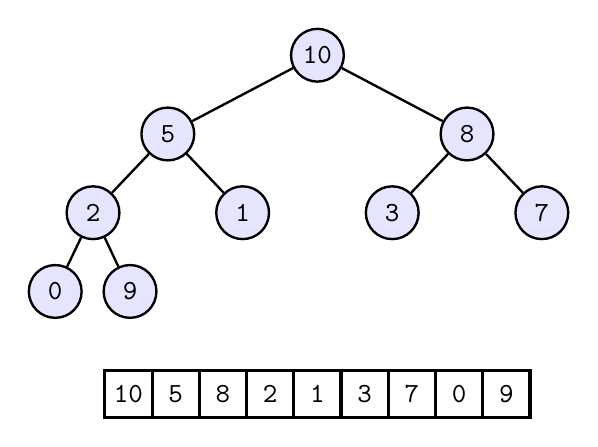
\begin{tikzpicture}

\fill[blue!10] (0.0, 0.0) circle (0.35);
\node [line width=0.03cm,black,minimum size=0.6699999999999999cm,draw,circle] at (0.0,0.0)(10){};\draw (0.0, 0.0) node[color=black] {\texttt{10}};
\fill[blue!10] (-1.9, -1.0) circle (0.35);
\node [line width=0.03cm,black,minimum size=0.6699999999999999cm,draw,circle] at (-1.9,-1.0)(5){};\draw (-1.9, -1.0) node[color=black] {\texttt{5}};
\fill[blue!10] (1.9, -1.0) circle (0.35);
\node [line width=0.03cm,black,minimum size=0.6699999999999999cm,draw,circle] at (1.9,-1.0)(8){};\draw (1.9, -1.0) node[color=black] {\texttt{8}};
\fill[blue!10] (-2.85, -2.0) circle (0.35);
\node [line width=0.03cm,black,minimum size=0.6699999999999999cm,draw,circle] at (-2.85,-2.0)(2){};\draw (-2.85, -2.0) node[color=black] {\texttt{2}};
\fill[blue!10] (-0.95, -2.0) circle (0.35);
\node [line width=0.03cm,black,minimum size=0.6699999999999999cm,draw,circle] at (-0.95,-2.0)(1){};\draw (-0.95, -2.0) node[color=black] {\texttt{1}};
\fill[blue!10] (0.95, -2.0) circle (0.35);
\node [line width=0.03cm,black,minimum size=0.6699999999999999cm,draw,circle] at (0.95,-2.0)(3){};\draw (0.95, -2.0) node[color=black] {\texttt{3}};
\fill[blue!10] (2.85, -2.0) circle (0.35);
\node [line width=0.03cm,black,minimum size=0.6699999999999999cm,draw,circle] at (2.85,-2.0)(7){};\draw (2.85, -2.0) node[color=black] {\texttt{7}};
\fill[blue!10] (-3.33, -3.0) circle (0.35);
\node [line width=0.03cm,black,minimum size=0.6699999999999999cm,draw,circle] at (-3.33,-3.0)(0){};\draw (-3.33, -3.0) node[color=black] {\texttt{0}};
\fill[blue!10] (-2.38, -3.0) circle (0.35);
\node [line width=0.03cm,black,minimum size=0.6699999999999999cm,draw,circle] at (-2.38,-3.0)(9){};\draw (-2.38, -3.0) node[color=black] {\texttt{9}};\draw[line width=0.03cm,black] (10) to  (5);
\draw[line width=0.03cm,black] (10) to  (8);
\draw[line width=0.03cm,black] (5) to  (2);
\draw[line width=0.03cm,black] (5) to  (1);
\draw[line width=0.03cm,black] (8) to  (3);
\draw[line width=0.03cm,black] (8) to  (7);
\draw[line width=0.03cm,black] (2) to  (0);
\draw[line width=0.03cm,black] (2) to  (9);

\draw (-2.3999999999999995, -4.299999999999999)
  node[draw, line width=0.04cm, , color=black,
       rounded corners=0cm, inner sep=0cm] {

\begin{minipage}[t][0.6cm]{0.6cm}
\mbox{}

\end{minipage}

};\draw (-2.3999999999999995, -4.299999999999999) node[color=black] {{\texttt{10}}};
\draw (-1.7999999999999996, -4.299999999999999)
  node[draw, line width=0.04cm, , color=black,
       rounded corners=0cm, inner sep=0cm] {

\begin{minipage}[t][0.6cm]{0.6cm}
\mbox{}

\end{minipage}

};\draw (-1.7999999999999996, -4.299999999999999) node[color=black] {{\texttt{5}}};
\draw (-1.1999999999999997, -4.299999999999999)
  node[draw, line width=0.04cm, , color=black,
       rounded corners=0cm, inner sep=0cm] {

\begin{minipage}[t][0.6cm]{0.6cm}
\mbox{}

\end{minipage}

};\draw (-1.1999999999999997, -4.299999999999999) node[color=black] {{\texttt{8}}};
\draw (-0.5999999999999996, -4.299999999999999)
  node[draw, line width=0.04cm, , color=black,
       rounded corners=0cm, inner sep=0cm] {

\begin{minipage}[t][0.6cm]{0.6cm}
\mbox{}

\end{minipage}

};\draw (-0.5999999999999996, -4.299999999999999) node[color=black] {{\texttt{2}}};
\draw (4.440892098500626e-16, -4.299999999999999)
  node[draw, line width=0.04cm, , color=black,
       rounded corners=0cm, inner sep=0cm] {

\begin{minipage}[t][0.6cm]{0.6cm}
\mbox{}

\end{minipage}

};\draw (4.440892098500626e-16, -4.299999999999999) node[color=black] {{\texttt{1}}};
\draw (0.6000000000000005, -4.299999999999999)
  node[draw, line width=0.04cm, , color=black,
       rounded corners=0cm, inner sep=0cm] {

\begin{minipage}[t][0.6cm]{0.6cm}
\mbox{}

\end{minipage}

};\draw (0.6000000000000005, -4.299999999999999) node[color=black] {{\texttt{3}}};
\draw (1.2000000000000006, -4.299999999999999)
  node[draw, line width=0.04cm, , color=black,
       rounded corners=0cm, inner sep=0cm] {

\begin{minipage}[t][0.6cm]{0.6cm}
\mbox{}

\end{minipage}

};\draw (1.2000000000000006, -4.299999999999999) node[color=black] {{\texttt{7}}};
\draw (1.8000000000000007, -4.299999999999999)
  node[draw, line width=0.04cm, , color=black,
       rounded corners=0cm, inner sep=0cm] {

\begin{minipage}[t][0.6cm]{0.6cm}
\mbox{}

\end{minipage}

};\draw (1.8000000000000007, -4.299999999999999) node[color=black] {{\texttt{0}}};
\draw (2.4000000000000004, -4.299999999999999)
  node[draw, line width=0.04cm, , color=black,
       rounded corners=0cm, inner sep=0cm] {

\begin{minipage}[t][0.6cm]{0.6cm}
\mbox{}

\end{minipage}

};\draw (2.4000000000000004, -4.299999999999999) node[color=black] {{\texttt{9}}};
\end{tikzpicture}

\end{center}



In the same manner, it shouldn't be too surprising that 
if we do an \lq\lq insert parent'' $o$ for $d$ in this tree:

%-*-latex-*-

\begin{center}
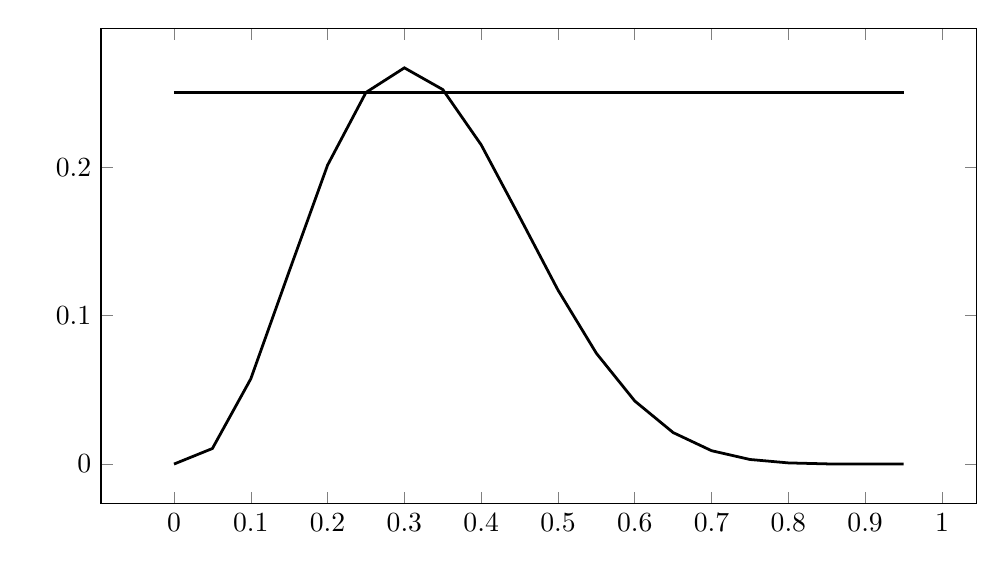
\begin{tikzpicture}[line width=1]
\begin{axis}[width=5in, height=3in,
             scatter/classes={a={mark=*,draw=black}},
             xlabel={\mbox{}},
             xlabel style={name=xlabel}, 
             ylabel={\mbox{}}, 
             legend style={
                at={(xlabel.south)},
                yshift=-1ex,
                anchor=north,
                legend cell align=left,
                },
        ]
]
\addplot[draw=black, line width=1] coordinates {(0.0, 0.0)
(0.05, 0.010475059441406248)
(0.1, 0.05739562800000002)
(0.15, 0.1298337207539062)
(0.2, 0.2013265920000001)
(0.25, 0.25028228759765625)
(0.3, 0.2668279319999998)
(0.35, 0.25221962497265626)
(0.4, 0.21499084799999998)
(0.45, 0.1664782928789064)
(0.5, 0.1171875)
(0.55, 0.07460310631640622)
(0.6, 0.042467328000000006)
(0.65, 0.02120301528515624)
(0.7, 0.009001692000000007)
(0.75, 0.00308990478515625)
(0.8, 0.000786431999999999)
(0.85, 0.0001259148164062501)
(0.9, 8.747999999999988e-06)
(0.95, 8.037890625000049e-08)};\addplot[draw=black, line width=1] coordinates {(0.0, 0.25)
(0.05, 0.25)
(0.1, 0.25)
(0.15, 0.25)
(0.2, 0.25)
(0.25, 0.25)
(0.3, 0.25)
(0.35, 0.25)
(0.4, 0.25)
(0.45, 0.25)
(0.5, 0.25)
(0.55, 0.25)
(0.6, 0.25)
(0.65, 0.25)
(0.7, 0.25)
(0.75, 0.25)
(0.8, 0.25)
(0.85, 0.25)
(0.9, 0.25)
(0.95, 0.25)};
\end{axis}\end{tikzpicture}\end{center}


that we get this:

%-*-latex-*-

\begin{center}
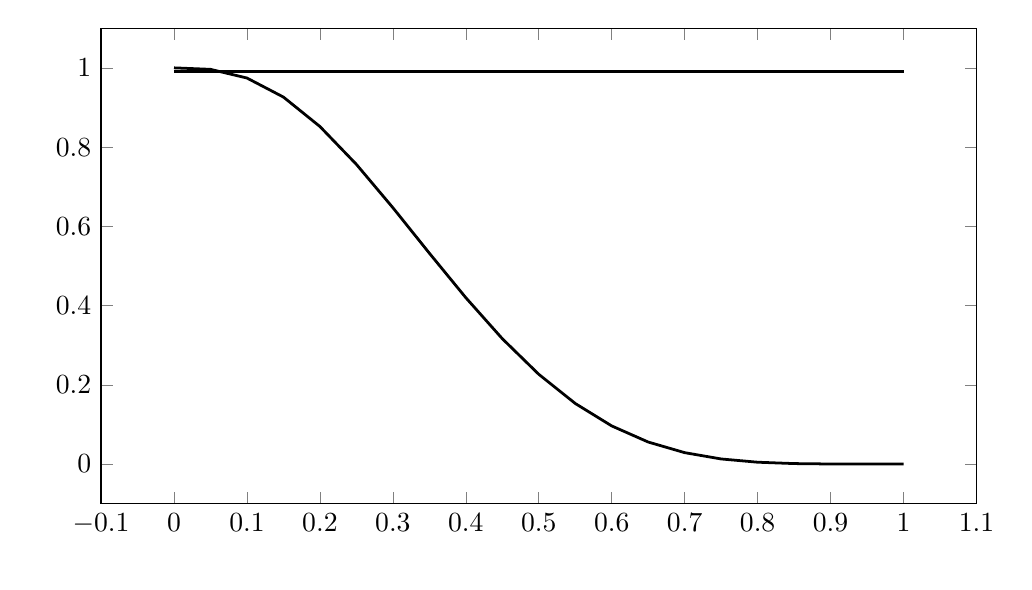
\begin{tikzpicture}[line width=1]
\begin{axis}[width=5in, height=3in,
             scatter/classes={a={mark=*,draw=black}},
             xlabel={\mbox{}},
             xlabel style={name=xlabel}, 
             ylabel={\mbox{}}, 
             legend style={
                at={(xlabel.south)},
                yshift=-1ex,
                anchor=north,
                legend cell align=left,
                },
        ]
]
\addplot[draw=black, line width=1] coordinates {(0.0, 1.0)
(0.05, 0.9962429570312497)
(0.1, 0.9743085000000002)
(0.15, 0.9262348398437498)
(0.2, 0.8519680000000004)
(0.25, 0.75640869140625)
(0.3, 0.6470694999999997)
(0.35, 0.53228332421875)
(0.4, 0.41990399999999994)
(0.45, 0.31644005078125015)
(0.5, 0.2265625)
(0.55, 0.15292768359374995)
(0.6, 0.09625600000000004)
(0.65, 0.055607535156249985)
(0.7, 0.02879550000000002)
(0.75, 0.01287841796875)
(0.8, 0.004671999999999996)
(0.85, 0.0012216445312500006)
(0.9, 0.00017649999999999982)
(0.95, 6.0273437500000275e-06)
(1.0, 0.0)};\addplot[draw=black, line width=1] coordinates {(0.0, 0.99)
(0.05, 0.99)
(0.1, 0.99)
(0.15, 0.99)
(0.2, 0.99)
(0.25, 0.99)
(0.3, 0.99)
(0.35, 0.99)
(0.4, 0.99)
(0.45, 0.99)
(0.5, 0.99)
(0.55, 0.99)
(0.6, 0.99)
(0.65, 0.99)
(0.7, 0.99)
(0.75, 0.99)
(0.8, 0.99)
(0.85, 0.99)
(0.9, 0.99)
(0.95, 0.99)
(1.0, 0.99)};
\end{axis}\end{tikzpicture}\end{center}


The above also makes sense if node $o$ has a left child.

\begin{Verbatim}[frame=single]
node.insert_parent(node2) make node2 the parent of node
                          and node2 the child of node's
                          original parent
node.insert(i, data)      create a new node for data and 
                          attach the new node as the i-th 
                          child of node. If there's already 
                          an i-th child, an exception is 
                          thrown.
node.insert(i, node2)     similar to above
node.insert_left(data)    create a new node for data and 
                          attach the new node to the left 
                          of node (this is for binary 
                          tree). If there's already a left 
                          child, an exception is thrown.
node.insert_left(node2)   Similar to above
node.insert_right(node2)  Similar to above.
\end{Verbatim}

For removal, we can
remove a single node that is a leaf.
I'll call this \verb!remove_leaf!.
Look at this:

\begin{center}
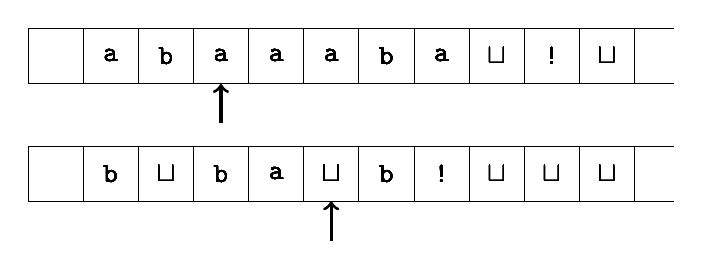
\begin{tikzpicture}

\draw (0.35, 0.35)
  node[draw, line width=0.01cm, , color=black,
       rounded corners=0cm, inner sep=0cm] {

\begin{minipage}[t][0.7cm]{0.7cm}
\mbox{}

\end{minipage}

};\draw (0.35, 0.35) node[color=black] {\texttt{\DOLLAR}};
\draw (1.0499999999999998, 0.35)
  node[draw, line width=0.01cm, , color=black,
       rounded corners=0cm, inner sep=0cm] {

\begin{minipage}[t][0.7cm]{0.7cm}
\mbox{}

\end{minipage}

};\draw (1.0499999999999998, 0.35) node[color=black] {\texttt{a}};
\draw (1.7499999999999998, 0.35)
  node[draw, line width=0.01cm, , color=black,
       rounded corners=0cm, inner sep=0cm] {

\begin{minipage}[t][0.7cm]{0.7cm}
\mbox{}

\end{minipage}

};\draw (1.7499999999999998, 0.35) node[color=black] {\texttt{b}};
\draw (2.4499999999999997, 0.35)
  node[draw, line width=0.01cm, , color=black,
       rounded corners=0cm, inner sep=0cm] {

\begin{minipage}[t][0.7cm]{0.7cm}
\mbox{}

\end{minipage}

};\draw (2.4499999999999997, 0.35) node[color=black] {\texttt{a}};
\draw (3.15, 0.35)
  node[draw, line width=0.01cm, , color=black,
       rounded corners=0cm, inner sep=0cm] {

\begin{minipage}[t][0.7cm]{0.7cm}
\mbox{}

\end{minipage}

};\draw (3.15, 0.35) node[color=black] {\texttt{a}};
\draw (3.85, 0.35)
  node[draw, line width=0.01cm, , color=black,
       rounded corners=0cm, inner sep=0cm] {

\begin{minipage}[t][0.7cm]{0.7cm}
\mbox{}

\end{minipage}

};\draw (3.85, 0.35) node[color=black] {\texttt{a}};
\draw (4.550000000000001, 0.35)
  node[draw, line width=0.01cm, , color=black,
       rounded corners=0cm, inner sep=0cm] {

\begin{minipage}[t][0.7cm]{0.7cm}
\mbox{}

\end{minipage}

};\draw (4.550000000000001, 0.35) node[color=black] {\texttt{b}};
\draw (5.25, 0.35)
  node[draw, line width=0.01cm, , color=black,
       rounded corners=0cm, inner sep=0cm] {

\begin{minipage}[t][0.7cm]{0.7cm}
\mbox{}

\end{minipage}

};\draw (5.25, 0.35) node[color=black] {\texttt{a}};
\draw (5.950000000000001, 0.35)
  node[draw, line width=0.01cm, , color=black,
       rounded corners=0cm, inner sep=0cm] {

\begin{minipage}[t][0.7cm]{0.7cm}
\mbox{}

\end{minipage}

};\draw (5.950000000000001, 0.35) node[color=black] {\texttt{$\sqcup$}};
\draw (6.65, 0.35)
  node[draw, line width=0.01cm, , color=black,
       rounded corners=0cm, inner sep=0cm] {

\begin{minipage}[t][0.7cm]{0.7cm}
\mbox{}

\end{minipage}

};\draw (6.65, 0.35) node[color=black] {\texttt{!}};
\draw (7.350000000000001, 0.35)
  node[draw, line width=0.01cm, , color=black,
       rounded corners=0cm, inner sep=0cm] {

\begin{minipage}[t][0.7cm]{0.7cm}
\mbox{}

\end{minipage}

};\draw (7.350000000000001, 0.35) node[color=black] {\texttt{$\sqcup$}};
\draw (0.35, 0.35)
  node[draw, line width=0.01cm, , color=black,
       rounded corners=0cm, inner sep=0cm] {

\begin{minipage}[t][0.7cm]{0.7cm}
\mbox{}

\end{minipage}

};\draw (0.35, 0.35) node[color=black] {\texttt{\DOLLAR}};
\draw (1.0499999999999998, 0.35)
  node[draw, line width=0.01cm, , color=black,
       rounded corners=0cm, inner sep=0cm] {

\begin{minipage}[t][0.7cm]{0.7cm}
\mbox{}

\end{minipage}

};\draw (1.0499999999999998, 0.35) node[color=black] {\texttt{a}};
\draw (1.7499999999999998, 0.35)
  node[draw, line width=0.01cm, , color=black,
       rounded corners=0cm, inner sep=0cm] {

\begin{minipage}[t][0.7cm]{0.7cm}
\mbox{}

\end{minipage}

};\draw (1.7499999999999998, 0.35) node[color=black] {\texttt{b}};
\draw (2.4499999999999997, 0.35)
  node[draw, line width=0.01cm, , color=black,
       rounded corners=0cm, inner sep=0cm] {

\begin{minipage}[t][0.7cm]{0.7cm}
\mbox{}

\end{minipage}

};\draw (2.4499999999999997, 0.35) node[color=black] {\texttt{a}};
\draw (3.15, 0.35)
  node[draw, line width=0.01cm, , color=black,
       rounded corners=0cm, inner sep=0cm] {

\begin{minipage}[t][0.7cm]{0.7cm}
\mbox{}

\end{minipage}

};\draw (3.15, 0.35) node[color=black] {\texttt{a}};
\draw (3.85, 0.35)
  node[draw, line width=0.01cm, , color=black,
       rounded corners=0cm, inner sep=0cm] {

\begin{minipage}[t][0.7cm]{0.7cm}
\mbox{}

\end{minipage}

};\draw (3.85, 0.35) node[color=black] {\texttt{a}};
\draw (4.550000000000001, 0.35)
  node[draw, line width=0.01cm, , color=black,
       rounded corners=0cm, inner sep=0cm] {

\begin{minipage}[t][0.7cm]{0.7cm}
\mbox{}

\end{minipage}

};\draw (4.550000000000001, 0.35) node[color=black] {\texttt{b}};
\draw (5.25, 0.35)
  node[draw, line width=0.01cm, , color=black,
       rounded corners=0cm, inner sep=0cm] {

\begin{minipage}[t][0.7cm]{0.7cm}
\mbox{}

\end{minipage}

};\draw (5.25, 0.35) node[color=black] {\texttt{a}};
\draw (5.950000000000001, 0.35)
  node[draw, line width=0.01cm, , color=black,
       rounded corners=0cm, inner sep=0cm] {

\begin{minipage}[t][0.7cm]{0.7cm}
\mbox{}

\end{minipage}

};\draw (5.950000000000001, 0.35) node[color=black] {\texttt{$\sqcup$}};
\draw (6.65, 0.35)
  node[draw, line width=0.01cm, , color=black,
       rounded corners=0cm, inner sep=0cm] {

\begin{minipage}[t][0.7cm]{0.7cm}
\mbox{}

\end{minipage}

};\draw (6.65, 0.35) node[color=black] {\texttt{!}};
\draw (7.350000000000001, 0.35)
  node[draw, line width=0.01cm, , color=black,
       rounded corners=0cm, inner sep=0cm] {

\begin{minipage}[t][0.7cm]{0.7cm}
\mbox{}

\end{minipage}

};\draw (7.350000000000001, 0.35) node[color=black] {\texttt{$\sqcup$}};
\draw (0.35, 0.35)
  node[draw, line width=0.01cm, , color=black,
       rounded corners=0cm, inner sep=0cm] {

\begin{minipage}[t][0.7cm]{0.7cm}
\mbox{}

\end{minipage}

};\draw (0.35, 0.35) node[color=black] {\texttt{\DOLLAR}};
\draw (1.0499999999999998, 0.35)
  node[draw, line width=0.01cm, , color=black,
       rounded corners=0cm, inner sep=0cm] {

\begin{minipage}[t][0.7cm]{0.7cm}
\mbox{}

\end{minipage}

};\draw (1.0499999999999998, 0.35) node[color=black] {\texttt{a}};
\draw (1.7499999999999998, 0.35)
  node[draw, line width=0.01cm, , color=black,
       rounded corners=0cm, inner sep=0cm] {

\begin{minipage}[t][0.7cm]{0.7cm}
\mbox{}

\end{minipage}

};\draw (1.7499999999999998, 0.35) node[color=black] {\texttt{b}};
\draw (2.4499999999999997, 0.35)
  node[draw, line width=0.01cm, , color=black,
       rounded corners=0cm, inner sep=0cm] {

\begin{minipage}[t][0.7cm]{0.7cm}
\mbox{}

\end{minipage}

};\draw (2.4499999999999997, 0.35) node[color=black] {\texttt{a}};
\draw (3.15, 0.35)
  node[draw, line width=0.01cm, , color=black,
       rounded corners=0cm, inner sep=0cm] {

\begin{minipage}[t][0.7cm]{0.7cm}
\mbox{}

\end{minipage}

};\draw (3.15, 0.35) node[color=black] {\texttt{a}};
\draw (3.85, 0.35)
  node[draw, line width=0.01cm, , color=black,
       rounded corners=0cm, inner sep=0cm] {

\begin{minipage}[t][0.7cm]{0.7cm}
\mbox{}

\end{minipage}

};\draw (3.85, 0.35) node[color=black] {\texttt{a}};
\draw (4.550000000000001, 0.35)
  node[draw, line width=0.01cm, , color=black,
       rounded corners=0cm, inner sep=0cm] {

\begin{minipage}[t][0.7cm]{0.7cm}
\mbox{}

\end{minipage}

};\draw (4.550000000000001, 0.35) node[color=black] {\texttt{b}};
\draw (5.25, 0.35)
  node[draw, line width=0.01cm, , color=black,
       rounded corners=0cm, inner sep=0cm] {

\begin{minipage}[t][0.7cm]{0.7cm}
\mbox{}

\end{minipage}

};\draw (5.25, 0.35) node[color=black] {\texttt{a}};
\draw (5.950000000000001, 0.35)
  node[draw, line width=0.01cm, , color=black,
       rounded corners=0cm, inner sep=0cm] {

\begin{minipage}[t][0.7cm]{0.7cm}
\mbox{}

\end{minipage}

};\draw (5.950000000000001, 0.35) node[color=black] {\texttt{$\sqcup$}};
\draw (6.65, 0.35)
  node[draw, line width=0.01cm, , color=black,
       rounded corners=0cm, inner sep=0cm] {

\begin{minipage}[t][0.7cm]{0.7cm}
\mbox{}

\end{minipage}

};\draw (6.65, 0.35) node[color=black] {\texttt{!}};
\draw (7.350000000000001, 0.35)
  node[draw, line width=0.01cm, , color=black,
       rounded corners=0cm, inner sep=0cm] {

\begin{minipage}[t][0.7cm]{0.7cm}
\mbox{}

\end{minipage}

};\draw (7.350000000000001, 0.35) node[color=black] {\texttt{$\sqcup$}};
\draw (0.35, 0.35)
  node[draw, line width=0.01cm, , color=black,
       rounded corners=0cm, inner sep=0cm] {

\begin{minipage}[t][0.7cm]{0.7cm}
\mbox{}

\end{minipage}

};\draw (0.35, 0.35) node[color=black] {\texttt{\DOLLAR}};
\draw (1.0499999999999998, 0.35)
  node[draw, line width=0.01cm, , color=black,
       rounded corners=0cm, inner sep=0cm] {

\begin{minipage}[t][0.7cm]{0.7cm}
\mbox{}

\end{minipage}

};\draw (1.0499999999999998, 0.35) node[color=black] {\texttt{a}};
\draw (1.7499999999999998, 0.35)
  node[draw, line width=0.01cm, , color=black,
       rounded corners=0cm, inner sep=0cm] {

\begin{minipage}[t][0.7cm]{0.7cm}
\mbox{}

\end{minipage}

};\draw (1.7499999999999998, 0.35) node[color=black] {\texttt{b}};
\draw (2.4499999999999997, 0.35)
  node[draw, line width=0.01cm, , color=black,
       rounded corners=0cm, inner sep=0cm] {

\begin{minipage}[t][0.7cm]{0.7cm}
\mbox{}

\end{minipage}

};\draw (2.4499999999999997, 0.35) node[color=black] {\texttt{a}};
\draw (3.15, 0.35)
  node[draw, line width=0.01cm, , color=black,
       rounded corners=0cm, inner sep=0cm] {

\begin{minipage}[t][0.7cm]{0.7cm}
\mbox{}

\end{minipage}

};\draw (3.15, 0.35) node[color=black] {\texttt{a}};
\draw (3.85, 0.35)
  node[draw, line width=0.01cm, , color=black,
       rounded corners=0cm, inner sep=0cm] {

\begin{minipage}[t][0.7cm]{0.7cm}
\mbox{}

\end{minipage}

};\draw (3.85, 0.35) node[color=black] {\texttt{a}};
\draw (4.550000000000001, 0.35)
  node[draw, line width=0.01cm, , color=black,
       rounded corners=0cm, inner sep=0cm] {

\begin{minipage}[t][0.7cm]{0.7cm}
\mbox{}

\end{minipage}

};\draw (4.550000000000001, 0.35) node[color=black] {\texttt{b}};
\draw (5.25, 0.35)
  node[draw, line width=0.01cm, , color=black,
       rounded corners=0cm, inner sep=0cm] {

\begin{minipage}[t][0.7cm]{0.7cm}
\mbox{}

\end{minipage}

};\draw (5.25, 0.35) node[color=black] {\texttt{a}};
\draw (5.950000000000001, 0.35)
  node[draw, line width=0.01cm, , color=black,
       rounded corners=0cm, inner sep=0cm] {

\begin{minipage}[t][0.7cm]{0.7cm}
\mbox{}

\end{minipage}

};\draw (5.950000000000001, 0.35) node[color=black] {\texttt{$\sqcup$}};
\draw (6.65, 0.35)
  node[draw, line width=0.01cm, , color=black,
       rounded corners=0cm, inner sep=0cm] {

\begin{minipage}[t][0.7cm]{0.7cm}
\mbox{}

\end{minipage}

};\draw (6.65, 0.35) node[color=black] {\texttt{!}};
\draw (7.350000000000001, 0.35)
  node[draw, line width=0.01cm, , color=black,
       rounded corners=0cm, inner sep=0cm] {

\begin{minipage}[t][0.7cm]{0.7cm}
\mbox{}

\end{minipage}

};\draw (7.350000000000001, 0.35) node[color=black] {\texttt{$\sqcup$}};
\draw (0.35, 0.35)
  node[draw, line width=0.01cm, , color=black,
       rounded corners=0cm, inner sep=0cm] {

\begin{minipage}[t][0.7cm]{0.7cm}
\mbox{}

\end{minipage}

};\draw (0.35, 0.35) node[color=black] {\texttt{\DOLLAR}};
\draw (1.0499999999999998, 0.35)
  node[draw, line width=0.01cm, , color=black,
       rounded corners=0cm, inner sep=0cm] {

\begin{minipage}[t][0.7cm]{0.7cm}
\mbox{}

\end{minipage}

};\draw (1.0499999999999998, 0.35) node[color=black] {\texttt{a}};
\draw (1.7499999999999998, 0.35)
  node[draw, line width=0.01cm, , color=black,
       rounded corners=0cm, inner sep=0cm] {

\begin{minipage}[t][0.7cm]{0.7cm}
\mbox{}

\end{minipage}

};\draw (1.7499999999999998, 0.35) node[color=black] {\texttt{b}};
\draw (2.4499999999999997, 0.35)
  node[draw, line width=0.01cm, , color=black,
       rounded corners=0cm, inner sep=0cm] {

\begin{minipage}[t][0.7cm]{0.7cm}
\mbox{}

\end{minipage}

};\draw (2.4499999999999997, 0.35) node[color=black] {\texttt{a}};
\draw (3.15, 0.35)
  node[draw, line width=0.01cm, , color=black,
       rounded corners=0cm, inner sep=0cm] {

\begin{minipage}[t][0.7cm]{0.7cm}
\mbox{}

\end{minipage}

};\draw (3.15, 0.35) node[color=black] {\texttt{a}};
\draw (3.85, 0.35)
  node[draw, line width=0.01cm, , color=black,
       rounded corners=0cm, inner sep=0cm] {

\begin{minipage}[t][0.7cm]{0.7cm}
\mbox{}

\end{minipage}

};\draw (3.85, 0.35) node[color=black] {\texttt{a}};
\draw (4.550000000000001, 0.35)
  node[draw, line width=0.01cm, , color=black,
       rounded corners=0cm, inner sep=0cm] {

\begin{minipage}[t][0.7cm]{0.7cm}
\mbox{}

\end{minipage}

};\draw (4.550000000000001, 0.35) node[color=black] {\texttt{b}};
\draw (5.25, 0.35)
  node[draw, line width=0.01cm, , color=black,
       rounded corners=0cm, inner sep=0cm] {

\begin{minipage}[t][0.7cm]{0.7cm}
\mbox{}

\end{minipage}

};\draw (5.25, 0.35) node[color=black] {\texttt{a}};
\draw (5.950000000000001, 0.35)
  node[draw, line width=0.01cm, , color=black,
       rounded corners=0cm, inner sep=0cm] {

\begin{minipage}[t][0.7cm]{0.7cm}
\mbox{}

\end{minipage}

};\draw (5.950000000000001, 0.35) node[color=black] {\texttt{$\sqcup$}};
\draw (6.65, 0.35)
  node[draw, line width=0.01cm, , color=black,
       rounded corners=0cm, inner sep=0cm] {

\begin{minipage}[t][0.7cm]{0.7cm}
\mbox{}

\end{minipage}

};\draw (6.65, 0.35) node[color=black] {\texttt{!}};
\draw (7.350000000000001, 0.35)
  node[draw, line width=0.01cm, , color=black,
       rounded corners=0cm, inner sep=0cm] {

\begin{minipage}[t][0.7cm]{0.7cm}
\mbox{}

\end{minipage}

};\draw (7.350000000000001, 0.35) node[color=black] {\texttt{$\sqcup$}};
\draw (0.35, 0.35)
  node[draw, line width=0.01cm, , color=black,
       rounded corners=0cm, inner sep=0cm] {

\begin{minipage}[t][0.7cm]{0.7cm}
\mbox{}

\end{minipage}

};\draw (0.35, 0.35) node[color=black] {\texttt{\DOLLAR}};
\draw (1.0499999999999998, 0.35)
  node[draw, line width=0.01cm, , color=black,
       rounded corners=0cm, inner sep=0cm] {

\begin{minipage}[t][0.7cm]{0.7cm}
\mbox{}

\end{minipage}

};\draw (1.0499999999999998, 0.35) node[color=black] {\texttt{a}};
\draw (1.7499999999999998, 0.35)
  node[draw, line width=0.01cm, , color=black,
       rounded corners=0cm, inner sep=0cm] {

\begin{minipage}[t][0.7cm]{0.7cm}
\mbox{}

\end{minipage}

};\draw (1.7499999999999998, 0.35) node[color=black] {\texttt{b}};
\draw (2.4499999999999997, 0.35)
  node[draw, line width=0.01cm, , color=black,
       rounded corners=0cm, inner sep=0cm] {

\begin{minipage}[t][0.7cm]{0.7cm}
\mbox{}

\end{minipage}

};\draw (2.4499999999999997, 0.35) node[color=black] {\texttt{a}};
\draw (3.15, 0.35)
  node[draw, line width=0.01cm, , color=black,
       rounded corners=0cm, inner sep=0cm] {

\begin{minipage}[t][0.7cm]{0.7cm}
\mbox{}

\end{minipage}

};\draw (3.15, 0.35) node[color=black] {\texttt{a}};
\draw (3.85, 0.35)
  node[draw, line width=0.01cm, , color=black,
       rounded corners=0cm, inner sep=0cm] {

\begin{minipage}[t][0.7cm]{0.7cm}
\mbox{}

\end{minipage}

};\draw (3.85, 0.35) node[color=black] {\texttt{a}};
\draw (4.550000000000001, 0.35)
  node[draw, line width=0.01cm, , color=black,
       rounded corners=0cm, inner sep=0cm] {

\begin{minipage}[t][0.7cm]{0.7cm}
\mbox{}

\end{minipage}

};\draw (4.550000000000001, 0.35) node[color=black] {\texttt{b}};
\draw (5.25, 0.35)
  node[draw, line width=0.01cm, , color=black,
       rounded corners=0cm, inner sep=0cm] {

\begin{minipage}[t][0.7cm]{0.7cm}
\mbox{}

\end{minipage}

};\draw (5.25, 0.35) node[color=black] {\texttt{a}};
\draw (5.950000000000001, 0.35)
  node[draw, line width=0.01cm, , color=black,
       rounded corners=0cm, inner sep=0cm] {

\begin{minipage}[t][0.7cm]{0.7cm}
\mbox{}

\end{minipage}

};\draw (5.950000000000001, 0.35) node[color=black] {\texttt{$\sqcup$}};
\draw (6.65, 0.35)
  node[draw, line width=0.01cm, , color=black,
       rounded corners=0cm, inner sep=0cm] {

\begin{minipage}[t][0.7cm]{0.7cm}
\mbox{}

\end{minipage}

};\draw (6.65, 0.35) node[color=black] {\texttt{!}};
\draw (7.350000000000001, 0.35)
  node[draw, line width=0.01cm, , color=black,
       rounded corners=0cm, inner sep=0cm] {

\begin{minipage}[t][0.7cm]{0.7cm}
\mbox{}

\end{minipage}

};\draw (7.350000000000001, 0.35) node[color=black] {\texttt{$\sqcup$}};
\draw (0.35, 0.35)
  node[draw, line width=0.01cm, , color=black,
       rounded corners=0cm, inner sep=0cm] {

\begin{minipage}[t][0.7cm]{0.7cm}
\mbox{}

\end{minipage}

};\draw (0.35, 0.35) node[color=black] {\texttt{\DOLLAR}};
\draw (1.0499999999999998, 0.35)
  node[draw, line width=0.01cm, , color=black,
       rounded corners=0cm, inner sep=0cm] {

\begin{minipage}[t][0.7cm]{0.7cm}
\mbox{}

\end{minipage}

};\draw (1.0499999999999998, 0.35) node[color=black] {\texttt{a}};
\draw (1.7499999999999998, 0.35)
  node[draw, line width=0.01cm, , color=black,
       rounded corners=0cm, inner sep=0cm] {

\begin{minipage}[t][0.7cm]{0.7cm}
\mbox{}

\end{minipage}

};\draw (1.7499999999999998, 0.35) node[color=black] {\texttt{b}};
\draw (2.4499999999999997, 0.35)
  node[draw, line width=0.01cm, , color=black,
       rounded corners=0cm, inner sep=0cm] {

\begin{minipage}[t][0.7cm]{0.7cm}
\mbox{}

\end{minipage}

};\draw (2.4499999999999997, 0.35) node[color=black] {\texttt{a}};
\draw (3.15, 0.35)
  node[draw, line width=0.01cm, , color=black,
       rounded corners=0cm, inner sep=0cm] {

\begin{minipage}[t][0.7cm]{0.7cm}
\mbox{}

\end{minipage}

};\draw (3.15, 0.35) node[color=black] {\texttt{a}};
\draw (3.85, 0.35)
  node[draw, line width=0.01cm, , color=black,
       rounded corners=0cm, inner sep=0cm] {

\begin{minipage}[t][0.7cm]{0.7cm}
\mbox{}

\end{minipage}

};\draw (3.85, 0.35) node[color=black] {\texttt{a}};
\draw (4.550000000000001, 0.35)
  node[draw, line width=0.01cm, , color=black,
       rounded corners=0cm, inner sep=0cm] {

\begin{minipage}[t][0.7cm]{0.7cm}
\mbox{}

\end{minipage}

};\draw (4.550000000000001, 0.35) node[color=black] {\texttt{b}};
\draw (5.25, 0.35)
  node[draw, line width=0.01cm, , color=black,
       rounded corners=0cm, inner sep=0cm] {

\begin{minipage}[t][0.7cm]{0.7cm}
\mbox{}

\end{minipage}

};\draw (5.25, 0.35) node[color=black] {\texttt{a}};
\draw (5.950000000000001, 0.35)
  node[draw, line width=0.01cm, , color=black,
       rounded corners=0cm, inner sep=0cm] {

\begin{minipage}[t][0.7cm]{0.7cm}
\mbox{}

\end{minipage}

};\draw (5.950000000000001, 0.35) node[color=black] {\texttt{$\sqcup$}};
\draw (6.65, 0.35)
  node[draw, line width=0.01cm, , color=black,
       rounded corners=0cm, inner sep=0cm] {

\begin{minipage}[t][0.7cm]{0.7cm}
\mbox{}

\end{minipage}

};\draw (6.65, 0.35) node[color=black] {\texttt{!}};
\draw (7.350000000000001, 0.35)
  node[draw, line width=0.01cm, , color=black,
       rounded corners=0cm, inner sep=0cm] {

\begin{minipage}[t][0.7cm]{0.7cm}
\mbox{}

\end{minipage}

};\draw (7.350000000000001, 0.35) node[color=black] {\texttt{$\sqcup$}};
\draw (0.35, 0.35)
  node[draw, line width=0.01cm, , color=black,
       rounded corners=0cm, inner sep=0cm] {

\begin{minipage}[t][0.7cm]{0.7cm}
\mbox{}

\end{minipage}

};\draw (0.35, 0.35) node[color=black] {\texttt{\DOLLAR}};
\draw (1.0499999999999998, 0.35)
  node[draw, line width=0.01cm, , color=black,
       rounded corners=0cm, inner sep=0cm] {

\begin{minipage}[t][0.7cm]{0.7cm}
\mbox{}

\end{minipage}

};\draw (1.0499999999999998, 0.35) node[color=black] {\texttt{a}};
\draw (1.7499999999999998, 0.35)
  node[draw, line width=0.01cm, , color=black,
       rounded corners=0cm, inner sep=0cm] {

\begin{minipage}[t][0.7cm]{0.7cm}
\mbox{}

\end{minipage}

};\draw (1.7499999999999998, 0.35) node[color=black] {\texttt{b}};
\draw (2.4499999999999997, 0.35)
  node[draw, line width=0.01cm, , color=black,
       rounded corners=0cm, inner sep=0cm] {

\begin{minipage}[t][0.7cm]{0.7cm}
\mbox{}

\end{minipage}

};\draw (2.4499999999999997, 0.35) node[color=black] {\texttt{a}};
\draw (3.15, 0.35)
  node[draw, line width=0.01cm, , color=black,
       rounded corners=0cm, inner sep=0cm] {

\begin{minipage}[t][0.7cm]{0.7cm}
\mbox{}

\end{minipage}

};\draw (3.15, 0.35) node[color=black] {\texttt{a}};
\draw (3.85, 0.35)
  node[draw, line width=0.01cm, , color=black,
       rounded corners=0cm, inner sep=0cm] {

\begin{minipage}[t][0.7cm]{0.7cm}
\mbox{}

\end{minipage}

};\draw (3.85, 0.35) node[color=black] {\texttt{a}};
\draw (4.550000000000001, 0.35)
  node[draw, line width=0.01cm, , color=black,
       rounded corners=0cm, inner sep=0cm] {

\begin{minipage}[t][0.7cm]{0.7cm}
\mbox{}

\end{minipage}

};\draw (4.550000000000001, 0.35) node[color=black] {\texttt{b}};
\draw (5.25, 0.35)
  node[draw, line width=0.01cm, , color=black,
       rounded corners=0cm, inner sep=0cm] {

\begin{minipage}[t][0.7cm]{0.7cm}
\mbox{}

\end{minipage}

};\draw (5.25, 0.35) node[color=black] {\texttt{a}};
\draw (5.950000000000001, 0.35)
  node[draw, line width=0.01cm, , color=black,
       rounded corners=0cm, inner sep=0cm] {

\begin{minipage}[t][0.7cm]{0.7cm}
\mbox{}

\end{minipage}

};\draw (5.950000000000001, 0.35) node[color=black] {\texttt{$\sqcup$}};
\draw (6.65, 0.35)
  node[draw, line width=0.01cm, , color=black,
       rounded corners=0cm, inner sep=0cm] {

\begin{minipage}[t][0.7cm]{0.7cm}
\mbox{}

\end{minipage}

};\draw (6.65, 0.35) node[color=black] {\texttt{!}};
\draw (7.350000000000001, 0.35)
  node[draw, line width=0.01cm, , color=black,
       rounded corners=0cm, inner sep=0cm] {

\begin{minipage}[t][0.7cm]{0.7cm}
\mbox{}

\end{minipage}

};\draw (7.350000000000001, 0.35) node[color=black] {\texttt{$\sqcup$}};
\draw (0.35, 0.35)
  node[draw, line width=0.01cm, , color=black,
       rounded corners=0cm, inner sep=0cm] {

\begin{minipage}[t][0.7cm]{0.7cm}
\mbox{}

\end{minipage}

};\draw (0.35, 0.35) node[color=black] {\texttt{\DOLLAR}};
\draw (1.0499999999999998, 0.35)
  node[draw, line width=0.01cm, , color=black,
       rounded corners=0cm, inner sep=0cm] {

\begin{minipage}[t][0.7cm]{0.7cm}
\mbox{}

\end{minipage}

};\draw (1.0499999999999998, 0.35) node[color=black] {\texttt{a}};
\draw (1.7499999999999998, 0.35)
  node[draw, line width=0.01cm, , color=black,
       rounded corners=0cm, inner sep=0cm] {

\begin{minipage}[t][0.7cm]{0.7cm}
\mbox{}

\end{minipage}

};\draw (1.7499999999999998, 0.35) node[color=black] {\texttt{b}};
\draw (2.4499999999999997, 0.35)
  node[draw, line width=0.01cm, , color=black,
       rounded corners=0cm, inner sep=0cm] {

\begin{minipage}[t][0.7cm]{0.7cm}
\mbox{}

\end{minipage}

};\draw (2.4499999999999997, 0.35) node[color=black] {\texttt{a}};
\draw (3.15, 0.35)
  node[draw, line width=0.01cm, , color=black,
       rounded corners=0cm, inner sep=0cm] {

\begin{minipage}[t][0.7cm]{0.7cm}
\mbox{}

\end{minipage}

};\draw (3.15, 0.35) node[color=black] {\texttt{a}};
\draw (3.85, 0.35)
  node[draw, line width=0.01cm, , color=black,
       rounded corners=0cm, inner sep=0cm] {

\begin{minipage}[t][0.7cm]{0.7cm}
\mbox{}

\end{minipage}

};\draw (3.85, 0.35) node[color=black] {\texttt{a}};
\draw (4.550000000000001, 0.35)
  node[draw, line width=0.01cm, , color=black,
       rounded corners=0cm, inner sep=0cm] {

\begin{minipage}[t][0.7cm]{0.7cm}
\mbox{}

\end{minipage}

};\draw (4.550000000000001, 0.35) node[color=black] {\texttt{b}};
\draw (5.25, 0.35)
  node[draw, line width=0.01cm, , color=black,
       rounded corners=0cm, inner sep=0cm] {

\begin{minipage}[t][0.7cm]{0.7cm}
\mbox{}

\end{minipage}

};\draw (5.25, 0.35) node[color=black] {\texttt{a}};
\draw (5.950000000000001, 0.35)
  node[draw, line width=0.01cm, , color=black,
       rounded corners=0cm, inner sep=0cm] {

\begin{minipage}[t][0.7cm]{0.7cm}
\mbox{}

\end{minipage}

};\draw (5.950000000000001, 0.35) node[color=black] {\texttt{$\sqcup$}};
\draw (6.65, 0.35)
  node[draw, line width=0.01cm, , color=black,
       rounded corners=0cm, inner sep=0cm] {

\begin{minipage}[t][0.7cm]{0.7cm}
\mbox{}

\end{minipage}

};\draw (6.65, 0.35) node[color=black] {\texttt{!}};
\draw (7.350000000000001, 0.35)
  node[draw, line width=0.01cm, , color=black,
       rounded corners=0cm, inner sep=0cm] {

\begin{minipage}[t][0.7cm]{0.7cm}
\mbox{}

\end{minipage}

};\draw (7.350000000000001, 0.35) node[color=black] {\texttt{$\sqcup$}};
\draw (0.35, 0.35)
  node[draw, line width=0.01cm, , color=black,
       rounded corners=0cm, inner sep=0cm] {

\begin{minipage}[t][0.7cm]{0.7cm}
\mbox{}

\end{minipage}

};\draw (0.35, 0.35) node[color=black] {\texttt{\DOLLAR}};
\draw (1.0499999999999998, 0.35)
  node[draw, line width=0.01cm, , color=black,
       rounded corners=0cm, inner sep=0cm] {

\begin{minipage}[t][0.7cm]{0.7cm}
\mbox{}

\end{minipage}

};\draw (1.0499999999999998, 0.35) node[color=black] {\texttt{a}};
\draw (1.7499999999999998, 0.35)
  node[draw, line width=0.01cm, , color=black,
       rounded corners=0cm, inner sep=0cm] {

\begin{minipage}[t][0.7cm]{0.7cm}
\mbox{}

\end{minipage}

};\draw (1.7499999999999998, 0.35) node[color=black] {\texttt{b}};
\draw (2.4499999999999997, 0.35)
  node[draw, line width=0.01cm, , color=black,
       rounded corners=0cm, inner sep=0cm] {

\begin{minipage}[t][0.7cm]{0.7cm}
\mbox{}

\end{minipage}

};\draw (2.4499999999999997, 0.35) node[color=black] {\texttt{a}};
\draw (3.15, 0.35)
  node[draw, line width=0.01cm, , color=black,
       rounded corners=0cm, inner sep=0cm] {

\begin{minipage}[t][0.7cm]{0.7cm}
\mbox{}

\end{minipage}

};\draw (3.15, 0.35) node[color=black] {\texttt{a}};
\draw (3.85, 0.35)
  node[draw, line width=0.01cm, , color=black,
       rounded corners=0cm, inner sep=0cm] {

\begin{minipage}[t][0.7cm]{0.7cm}
\mbox{}

\end{minipage}

};\draw (3.85, 0.35) node[color=black] {\texttt{a}};
\draw (4.550000000000001, 0.35)
  node[draw, line width=0.01cm, , color=black,
       rounded corners=0cm, inner sep=0cm] {

\begin{minipage}[t][0.7cm]{0.7cm}
\mbox{}

\end{minipage}

};\draw (4.550000000000001, 0.35) node[color=black] {\texttt{b}};
\draw (5.25, 0.35)
  node[draw, line width=0.01cm, , color=black,
       rounded corners=0cm, inner sep=0cm] {

\begin{minipage}[t][0.7cm]{0.7cm}
\mbox{}

\end{minipage}

};\draw (5.25, 0.35) node[color=black] {\texttt{a}};
\draw (5.950000000000001, 0.35)
  node[draw, line width=0.01cm, , color=black,
       rounded corners=0cm, inner sep=0cm] {

\begin{minipage}[t][0.7cm]{0.7cm}
\mbox{}

\end{minipage}

};\draw (5.950000000000001, 0.35) node[color=black] {\texttt{$\sqcup$}};
\draw (6.65, 0.35)
  node[draw, line width=0.01cm, , color=black,
       rounded corners=0cm, inner sep=0cm] {

\begin{minipage}[t][0.7cm]{0.7cm}
\mbox{}

\end{minipage}

};\draw (6.65, 0.35) node[color=black] {\texttt{!}};
\draw (7.350000000000001, 0.35)
  node[draw, line width=0.01cm, , color=black,
       rounded corners=0cm, inner sep=0cm] {

\begin{minipage}[t][0.7cm]{0.7cm}
\mbox{}

\end{minipage}

};\draw (7.350000000000001, 0.35) node[color=black] {\texttt{$\sqcup$}};
\draw (0.35, 0.35)
  node[draw, line width=0.01cm, , color=black,
       rounded corners=0cm, inner sep=0cm] {

\begin{minipage}[t][0.7cm]{0.7cm}
\mbox{}

\end{minipage}

};\draw (0.35, 0.35) node[color=black] {\texttt{\DOLLAR}};
\draw (1.0499999999999998, 0.35)
  node[draw, line width=0.01cm, , color=black,
       rounded corners=0cm, inner sep=0cm] {

\begin{minipage}[t][0.7cm]{0.7cm}
\mbox{}

\end{minipage}

};\draw (1.0499999999999998, 0.35) node[color=black] {\texttt{a}};
\draw (1.7499999999999998, 0.35)
  node[draw, line width=0.01cm, , color=black,
       rounded corners=0cm, inner sep=0cm] {

\begin{minipage}[t][0.7cm]{0.7cm}
\mbox{}

\end{minipage}

};\draw (1.7499999999999998, 0.35) node[color=black] {\texttt{b}};
\draw (2.4499999999999997, 0.35)
  node[draw, line width=0.01cm, , color=black,
       rounded corners=0cm, inner sep=0cm] {

\begin{minipage}[t][0.7cm]{0.7cm}
\mbox{}

\end{minipage}

};\draw (2.4499999999999997, 0.35) node[color=black] {\texttt{a}};
\draw (3.15, 0.35)
  node[draw, line width=0.01cm, , color=black,
       rounded corners=0cm, inner sep=0cm] {

\begin{minipage}[t][0.7cm]{0.7cm}
\mbox{}

\end{minipage}

};\draw (3.15, 0.35) node[color=black] {\texttt{a}};
\draw (3.85, 0.35)
  node[draw, line width=0.01cm, , color=black,
       rounded corners=0cm, inner sep=0cm] {

\begin{minipage}[t][0.7cm]{0.7cm}
\mbox{}

\end{minipage}

};\draw (3.85, 0.35) node[color=black] {\texttt{a}};
\draw (4.550000000000001, 0.35)
  node[draw, line width=0.01cm, , color=black,
       rounded corners=0cm, inner sep=0cm] {

\begin{minipage}[t][0.7cm]{0.7cm}
\mbox{}

\end{minipage}

};\draw (4.550000000000001, 0.35) node[color=black] {\texttt{b}};
\draw (5.25, 0.35)
  node[draw, line width=0.01cm, , color=black,
       rounded corners=0cm, inner sep=0cm] {

\begin{minipage}[t][0.7cm]{0.7cm}
\mbox{}

\end{minipage}

};\draw (5.25, 0.35) node[color=black] {\texttt{a}};
\draw (5.950000000000001, 0.35)
  node[draw, line width=0.01cm, , color=black,
       rounded corners=0cm, inner sep=0cm] {

\begin{minipage}[t][0.7cm]{0.7cm}
\mbox{}

\end{minipage}

};\draw (5.950000000000001, 0.35) node[color=black] {\texttt{$\sqcup$}};
\draw (6.65, 0.35)
  node[draw, line width=0.01cm, , color=black,
       rounded corners=0cm, inner sep=0cm] {

\begin{minipage}[t][0.7cm]{0.7cm}
\mbox{}

\end{minipage}

};\draw (6.65, 0.35) node[color=black] {\texttt{!}};
\draw (7.350000000000001, 0.35)
  node[draw, line width=0.01cm, , color=black,
       rounded corners=0cm, inner sep=0cm] {

\begin{minipage}[t][0.7cm]{0.7cm}
\mbox{}

\end{minipage}

};\draw (7.350000000000001, 0.35) node[color=black] {\texttt{$\sqcup$}};\draw[line width=0.01cm,black] (7.700000000000001,0.7) to  (8.200000000000001,0.7);
\draw[line width=0.01cm,black] (7.700000000000001,0.0) to  (8.200000000000001,0.0);
\draw[line width=0.04cm,black,->] (2.45,-0.51) to  (2.45,-0.01);

\draw (0.35, -1.15)
  node[draw, line width=0.01cm, , color=black,
       rounded corners=0cm, inner sep=0cm] {

\begin{minipage}[t][0.7cm]{0.7cm}
\mbox{}

\end{minipage}

};\draw (0.35, -1.15) node[color=black] {\texttt{\DOLLAR}};
\draw (1.0499999999999998, -1.15)
  node[draw, line width=0.01cm, , color=black,
       rounded corners=0cm, inner sep=0cm] {

\begin{minipage}[t][0.7cm]{0.7cm}
\mbox{}

\end{minipage}

};\draw (1.0499999999999998, -1.15) node[color=black] {\texttt{b}};
\draw (1.7499999999999998, -1.15)
  node[draw, line width=0.01cm, , color=black,
       rounded corners=0cm, inner sep=0cm] {

\begin{minipage}[t][0.7cm]{0.7cm}
\mbox{}

\end{minipage}

};\draw (1.7499999999999998, -1.15) node[color=black] {\texttt{$\sqcup$}};
\draw (2.4499999999999997, -1.15)
  node[draw, line width=0.01cm, , color=black,
       rounded corners=0cm, inner sep=0cm] {

\begin{minipage}[t][0.7cm]{0.7cm}
\mbox{}

\end{minipage}

};\draw (2.4499999999999997, -1.15) node[color=black] {\texttt{b}};
\draw (3.15, -1.15)
  node[draw, line width=0.01cm, , color=black,
       rounded corners=0cm, inner sep=0cm] {

\begin{minipage}[t][0.7cm]{0.7cm}
\mbox{}

\end{minipage}

};\draw (3.15, -1.15) node[color=black] {\texttt{a}};
\draw (3.85, -1.15)
  node[draw, line width=0.01cm, , color=black,
       rounded corners=0cm, inner sep=0cm] {

\begin{minipage}[t][0.7cm]{0.7cm}
\mbox{}

\end{minipage}

};\draw (3.85, -1.15) node[color=black] {\texttt{$\sqcup$}};
\draw (4.550000000000001, -1.15)
  node[draw, line width=0.01cm, , color=black,
       rounded corners=0cm, inner sep=0cm] {

\begin{minipage}[t][0.7cm]{0.7cm}
\mbox{}

\end{minipage}

};\draw (4.550000000000001, -1.15) node[color=black] {\texttt{b}};
\draw (5.25, -1.15)
  node[draw, line width=0.01cm, , color=black,
       rounded corners=0cm, inner sep=0cm] {

\begin{minipage}[t][0.7cm]{0.7cm}
\mbox{}

\end{minipage}

};\draw (5.25, -1.15) node[color=black] {\texttt{!}};
\draw (5.950000000000001, -1.15)
  node[draw, line width=0.01cm, , color=black,
       rounded corners=0cm, inner sep=0cm] {

\begin{minipage}[t][0.7cm]{0.7cm}
\mbox{}

\end{minipage}

};\draw (5.950000000000001, -1.15) node[color=black] {\texttt{$\sqcup$}};
\draw (6.65, -1.15)
  node[draw, line width=0.01cm, , color=black,
       rounded corners=0cm, inner sep=0cm] {

\begin{minipage}[t][0.7cm]{0.7cm}
\mbox{}

\end{minipage}

};\draw (6.65, -1.15) node[color=black] {\texttt{$\sqcup$}};
\draw (7.350000000000001, -1.15)
  node[draw, line width=0.01cm, , color=black,
       rounded corners=0cm, inner sep=0cm] {

\begin{minipage}[t][0.7cm]{0.7cm}
\mbox{}

\end{minipage}

};\draw (7.350000000000001, -1.15) node[color=black] {\texttt{$\sqcup$}};
\draw (0.35, -1.15)
  node[draw, line width=0.01cm, , color=black,
       rounded corners=0cm, inner sep=0cm] {

\begin{minipage}[t][0.7cm]{0.7cm}
\mbox{}

\end{minipage}

};\draw (0.35, -1.15) node[color=black] {\texttt{\DOLLAR}};
\draw (1.0499999999999998, -1.15)
  node[draw, line width=0.01cm, , color=black,
       rounded corners=0cm, inner sep=0cm] {

\begin{minipage}[t][0.7cm]{0.7cm}
\mbox{}

\end{minipage}

};\draw (1.0499999999999998, -1.15) node[color=black] {\texttt{b}};
\draw (1.7499999999999998, -1.15)
  node[draw, line width=0.01cm, , color=black,
       rounded corners=0cm, inner sep=0cm] {

\begin{minipage}[t][0.7cm]{0.7cm}
\mbox{}

\end{minipage}

};\draw (1.7499999999999998, -1.15) node[color=black] {\texttt{$\sqcup$}};
\draw (2.4499999999999997, -1.15)
  node[draw, line width=0.01cm, , color=black,
       rounded corners=0cm, inner sep=0cm] {

\begin{minipage}[t][0.7cm]{0.7cm}
\mbox{}

\end{minipage}

};\draw (2.4499999999999997, -1.15) node[color=black] {\texttt{b}};
\draw (3.15, -1.15)
  node[draw, line width=0.01cm, , color=black,
       rounded corners=0cm, inner sep=0cm] {

\begin{minipage}[t][0.7cm]{0.7cm}
\mbox{}

\end{minipage}

};\draw (3.15, -1.15) node[color=black] {\texttt{a}};
\draw (3.85, -1.15)
  node[draw, line width=0.01cm, , color=black,
       rounded corners=0cm, inner sep=0cm] {

\begin{minipage}[t][0.7cm]{0.7cm}
\mbox{}

\end{minipage}

};\draw (3.85, -1.15) node[color=black] {\texttt{$\sqcup$}};
\draw (4.550000000000001, -1.15)
  node[draw, line width=0.01cm, , color=black,
       rounded corners=0cm, inner sep=0cm] {

\begin{minipage}[t][0.7cm]{0.7cm}
\mbox{}

\end{minipage}

};\draw (4.550000000000001, -1.15) node[color=black] {\texttt{b}};
\draw (5.25, -1.15)
  node[draw, line width=0.01cm, , color=black,
       rounded corners=0cm, inner sep=0cm] {

\begin{minipage}[t][0.7cm]{0.7cm}
\mbox{}

\end{minipage}

};\draw (5.25, -1.15) node[color=black] {\texttt{!}};
\draw (5.950000000000001, -1.15)
  node[draw, line width=0.01cm, , color=black,
       rounded corners=0cm, inner sep=0cm] {

\begin{minipage}[t][0.7cm]{0.7cm}
\mbox{}

\end{minipage}

};\draw (5.950000000000001, -1.15) node[color=black] {\texttt{$\sqcup$}};
\draw (6.65, -1.15)
  node[draw, line width=0.01cm, , color=black,
       rounded corners=0cm, inner sep=0cm] {

\begin{minipage}[t][0.7cm]{0.7cm}
\mbox{}

\end{minipage}

};\draw (6.65, -1.15) node[color=black] {\texttt{$\sqcup$}};
\draw (7.350000000000001, -1.15)
  node[draw, line width=0.01cm, , color=black,
       rounded corners=0cm, inner sep=0cm] {

\begin{minipage}[t][0.7cm]{0.7cm}
\mbox{}

\end{minipage}

};\draw (7.350000000000001, -1.15) node[color=black] {\texttt{$\sqcup$}};
\draw (0.35, -1.15)
  node[draw, line width=0.01cm, , color=black,
       rounded corners=0cm, inner sep=0cm] {

\begin{minipage}[t][0.7cm]{0.7cm}
\mbox{}

\end{minipage}

};\draw (0.35, -1.15) node[color=black] {\texttt{\DOLLAR}};
\draw (1.0499999999999998, -1.15)
  node[draw, line width=0.01cm, , color=black,
       rounded corners=0cm, inner sep=0cm] {

\begin{minipage}[t][0.7cm]{0.7cm}
\mbox{}

\end{minipage}

};\draw (1.0499999999999998, -1.15) node[color=black] {\texttt{b}};
\draw (1.7499999999999998, -1.15)
  node[draw, line width=0.01cm, , color=black,
       rounded corners=0cm, inner sep=0cm] {

\begin{minipage}[t][0.7cm]{0.7cm}
\mbox{}

\end{minipage}

};\draw (1.7499999999999998, -1.15) node[color=black] {\texttt{$\sqcup$}};
\draw (2.4499999999999997, -1.15)
  node[draw, line width=0.01cm, , color=black,
       rounded corners=0cm, inner sep=0cm] {

\begin{minipage}[t][0.7cm]{0.7cm}
\mbox{}

\end{minipage}

};\draw (2.4499999999999997, -1.15) node[color=black] {\texttt{b}};
\draw (3.15, -1.15)
  node[draw, line width=0.01cm, , color=black,
       rounded corners=0cm, inner sep=0cm] {

\begin{minipage}[t][0.7cm]{0.7cm}
\mbox{}

\end{minipage}

};\draw (3.15, -1.15) node[color=black] {\texttt{a}};
\draw (3.85, -1.15)
  node[draw, line width=0.01cm, , color=black,
       rounded corners=0cm, inner sep=0cm] {

\begin{minipage}[t][0.7cm]{0.7cm}
\mbox{}

\end{minipage}

};\draw (3.85, -1.15) node[color=black] {\texttt{$\sqcup$}};
\draw (4.550000000000001, -1.15)
  node[draw, line width=0.01cm, , color=black,
       rounded corners=0cm, inner sep=0cm] {

\begin{minipage}[t][0.7cm]{0.7cm}
\mbox{}

\end{minipage}

};\draw (4.550000000000001, -1.15) node[color=black] {\texttt{b}};
\draw (5.25, -1.15)
  node[draw, line width=0.01cm, , color=black,
       rounded corners=0cm, inner sep=0cm] {

\begin{minipage}[t][0.7cm]{0.7cm}
\mbox{}

\end{minipage}

};\draw (5.25, -1.15) node[color=black] {\texttt{!}};
\draw (5.950000000000001, -1.15)
  node[draw, line width=0.01cm, , color=black,
       rounded corners=0cm, inner sep=0cm] {

\begin{minipage}[t][0.7cm]{0.7cm}
\mbox{}

\end{minipage}

};\draw (5.950000000000001, -1.15) node[color=black] {\texttt{$\sqcup$}};
\draw (6.65, -1.15)
  node[draw, line width=0.01cm, , color=black,
       rounded corners=0cm, inner sep=0cm] {

\begin{minipage}[t][0.7cm]{0.7cm}
\mbox{}

\end{minipage}

};\draw (6.65, -1.15) node[color=black] {\texttt{$\sqcup$}};
\draw (7.350000000000001, -1.15)
  node[draw, line width=0.01cm, , color=black,
       rounded corners=0cm, inner sep=0cm] {

\begin{minipage}[t][0.7cm]{0.7cm}
\mbox{}

\end{minipage}

};\draw (7.350000000000001, -1.15) node[color=black] {\texttt{$\sqcup$}};
\draw (0.35, -1.15)
  node[draw, line width=0.01cm, , color=black,
       rounded corners=0cm, inner sep=0cm] {

\begin{minipage}[t][0.7cm]{0.7cm}
\mbox{}

\end{minipage}

};\draw (0.35, -1.15) node[color=black] {\texttt{\DOLLAR}};
\draw (1.0499999999999998, -1.15)
  node[draw, line width=0.01cm, , color=black,
       rounded corners=0cm, inner sep=0cm] {

\begin{minipage}[t][0.7cm]{0.7cm}
\mbox{}

\end{minipage}

};\draw (1.0499999999999998, -1.15) node[color=black] {\texttt{b}};
\draw (1.7499999999999998, -1.15)
  node[draw, line width=0.01cm, , color=black,
       rounded corners=0cm, inner sep=0cm] {

\begin{minipage}[t][0.7cm]{0.7cm}
\mbox{}

\end{minipage}

};\draw (1.7499999999999998, -1.15) node[color=black] {\texttt{$\sqcup$}};
\draw (2.4499999999999997, -1.15)
  node[draw, line width=0.01cm, , color=black,
       rounded corners=0cm, inner sep=0cm] {

\begin{minipage}[t][0.7cm]{0.7cm}
\mbox{}

\end{minipage}

};\draw (2.4499999999999997, -1.15) node[color=black] {\texttt{b}};
\draw (3.15, -1.15)
  node[draw, line width=0.01cm, , color=black,
       rounded corners=0cm, inner sep=0cm] {

\begin{minipage}[t][0.7cm]{0.7cm}
\mbox{}

\end{minipage}

};\draw (3.15, -1.15) node[color=black] {\texttt{a}};
\draw (3.85, -1.15)
  node[draw, line width=0.01cm, , color=black,
       rounded corners=0cm, inner sep=0cm] {

\begin{minipage}[t][0.7cm]{0.7cm}
\mbox{}

\end{minipage}

};\draw (3.85, -1.15) node[color=black] {\texttt{$\sqcup$}};
\draw (4.550000000000001, -1.15)
  node[draw, line width=0.01cm, , color=black,
       rounded corners=0cm, inner sep=0cm] {

\begin{minipage}[t][0.7cm]{0.7cm}
\mbox{}

\end{minipage}

};\draw (4.550000000000001, -1.15) node[color=black] {\texttt{b}};
\draw (5.25, -1.15)
  node[draw, line width=0.01cm, , color=black,
       rounded corners=0cm, inner sep=0cm] {

\begin{minipage}[t][0.7cm]{0.7cm}
\mbox{}

\end{minipage}

};\draw (5.25, -1.15) node[color=black] {\texttt{!}};
\draw (5.950000000000001, -1.15)
  node[draw, line width=0.01cm, , color=black,
       rounded corners=0cm, inner sep=0cm] {

\begin{minipage}[t][0.7cm]{0.7cm}
\mbox{}

\end{minipage}

};\draw (5.950000000000001, -1.15) node[color=black] {\texttt{$\sqcup$}};
\draw (6.65, -1.15)
  node[draw, line width=0.01cm, , color=black,
       rounded corners=0cm, inner sep=0cm] {

\begin{minipage}[t][0.7cm]{0.7cm}
\mbox{}

\end{minipage}

};\draw (6.65, -1.15) node[color=black] {\texttt{$\sqcup$}};
\draw (7.350000000000001, -1.15)
  node[draw, line width=0.01cm, , color=black,
       rounded corners=0cm, inner sep=0cm] {

\begin{minipage}[t][0.7cm]{0.7cm}
\mbox{}

\end{minipage}

};\draw (7.350000000000001, -1.15) node[color=black] {\texttt{$\sqcup$}};
\draw (0.35, -1.15)
  node[draw, line width=0.01cm, , color=black,
       rounded corners=0cm, inner sep=0cm] {

\begin{minipage}[t][0.7cm]{0.7cm}
\mbox{}

\end{minipage}

};\draw (0.35, -1.15) node[color=black] {\texttt{\DOLLAR}};
\draw (1.0499999999999998, -1.15)
  node[draw, line width=0.01cm, , color=black,
       rounded corners=0cm, inner sep=0cm] {

\begin{minipage}[t][0.7cm]{0.7cm}
\mbox{}

\end{minipage}

};\draw (1.0499999999999998, -1.15) node[color=black] {\texttt{b}};
\draw (1.7499999999999998, -1.15)
  node[draw, line width=0.01cm, , color=black,
       rounded corners=0cm, inner sep=0cm] {

\begin{minipage}[t][0.7cm]{0.7cm}
\mbox{}

\end{minipage}

};\draw (1.7499999999999998, -1.15) node[color=black] {\texttt{$\sqcup$}};
\draw (2.4499999999999997, -1.15)
  node[draw, line width=0.01cm, , color=black,
       rounded corners=0cm, inner sep=0cm] {

\begin{minipage}[t][0.7cm]{0.7cm}
\mbox{}

\end{minipage}

};\draw (2.4499999999999997, -1.15) node[color=black] {\texttt{b}};
\draw (3.15, -1.15)
  node[draw, line width=0.01cm, , color=black,
       rounded corners=0cm, inner sep=0cm] {

\begin{minipage}[t][0.7cm]{0.7cm}
\mbox{}

\end{minipage}

};\draw (3.15, -1.15) node[color=black] {\texttt{a}};
\draw (3.85, -1.15)
  node[draw, line width=0.01cm, , color=black,
       rounded corners=0cm, inner sep=0cm] {

\begin{minipage}[t][0.7cm]{0.7cm}
\mbox{}

\end{minipage}

};\draw (3.85, -1.15) node[color=black] {\texttt{$\sqcup$}};
\draw (4.550000000000001, -1.15)
  node[draw, line width=0.01cm, , color=black,
       rounded corners=0cm, inner sep=0cm] {

\begin{minipage}[t][0.7cm]{0.7cm}
\mbox{}

\end{minipage}

};\draw (4.550000000000001, -1.15) node[color=black] {\texttt{b}};
\draw (5.25, -1.15)
  node[draw, line width=0.01cm, , color=black,
       rounded corners=0cm, inner sep=0cm] {

\begin{minipage}[t][0.7cm]{0.7cm}
\mbox{}

\end{minipage}

};\draw (5.25, -1.15) node[color=black] {\texttt{!}};
\draw (5.950000000000001, -1.15)
  node[draw, line width=0.01cm, , color=black,
       rounded corners=0cm, inner sep=0cm] {

\begin{minipage}[t][0.7cm]{0.7cm}
\mbox{}

\end{minipage}

};\draw (5.950000000000001, -1.15) node[color=black] {\texttt{$\sqcup$}};
\draw (6.65, -1.15)
  node[draw, line width=0.01cm, , color=black,
       rounded corners=0cm, inner sep=0cm] {

\begin{minipage}[t][0.7cm]{0.7cm}
\mbox{}

\end{minipage}

};\draw (6.65, -1.15) node[color=black] {\texttt{$\sqcup$}};
\draw (7.350000000000001, -1.15)
  node[draw, line width=0.01cm, , color=black,
       rounded corners=0cm, inner sep=0cm] {

\begin{minipage}[t][0.7cm]{0.7cm}
\mbox{}

\end{minipage}

};\draw (7.350000000000001, -1.15) node[color=black] {\texttt{$\sqcup$}};
\draw (0.35, -1.15)
  node[draw, line width=0.01cm, , color=black,
       rounded corners=0cm, inner sep=0cm] {

\begin{minipage}[t][0.7cm]{0.7cm}
\mbox{}

\end{minipage}

};\draw (0.35, -1.15) node[color=black] {\texttt{\DOLLAR}};
\draw (1.0499999999999998, -1.15)
  node[draw, line width=0.01cm, , color=black,
       rounded corners=0cm, inner sep=0cm] {

\begin{minipage}[t][0.7cm]{0.7cm}
\mbox{}

\end{minipage}

};\draw (1.0499999999999998, -1.15) node[color=black] {\texttt{b}};
\draw (1.7499999999999998, -1.15)
  node[draw, line width=0.01cm, , color=black,
       rounded corners=0cm, inner sep=0cm] {

\begin{minipage}[t][0.7cm]{0.7cm}
\mbox{}

\end{minipage}

};\draw (1.7499999999999998, -1.15) node[color=black] {\texttt{$\sqcup$}};
\draw (2.4499999999999997, -1.15)
  node[draw, line width=0.01cm, , color=black,
       rounded corners=0cm, inner sep=0cm] {

\begin{minipage}[t][0.7cm]{0.7cm}
\mbox{}

\end{minipage}

};\draw (2.4499999999999997, -1.15) node[color=black] {\texttt{b}};
\draw (3.15, -1.15)
  node[draw, line width=0.01cm, , color=black,
       rounded corners=0cm, inner sep=0cm] {

\begin{minipage}[t][0.7cm]{0.7cm}
\mbox{}

\end{minipage}

};\draw (3.15, -1.15) node[color=black] {\texttt{a}};
\draw (3.85, -1.15)
  node[draw, line width=0.01cm, , color=black,
       rounded corners=0cm, inner sep=0cm] {

\begin{minipage}[t][0.7cm]{0.7cm}
\mbox{}

\end{minipage}

};\draw (3.85, -1.15) node[color=black] {\texttt{$\sqcup$}};
\draw (4.550000000000001, -1.15)
  node[draw, line width=0.01cm, , color=black,
       rounded corners=0cm, inner sep=0cm] {

\begin{minipage}[t][0.7cm]{0.7cm}
\mbox{}

\end{minipage}

};\draw (4.550000000000001, -1.15) node[color=black] {\texttt{b}};
\draw (5.25, -1.15)
  node[draw, line width=0.01cm, , color=black,
       rounded corners=0cm, inner sep=0cm] {

\begin{minipage}[t][0.7cm]{0.7cm}
\mbox{}

\end{minipage}

};\draw (5.25, -1.15) node[color=black] {\texttt{!}};
\draw (5.950000000000001, -1.15)
  node[draw, line width=0.01cm, , color=black,
       rounded corners=0cm, inner sep=0cm] {

\begin{minipage}[t][0.7cm]{0.7cm}
\mbox{}

\end{minipage}

};\draw (5.950000000000001, -1.15) node[color=black] {\texttt{$\sqcup$}};
\draw (6.65, -1.15)
  node[draw, line width=0.01cm, , color=black,
       rounded corners=0cm, inner sep=0cm] {

\begin{minipage}[t][0.7cm]{0.7cm}
\mbox{}

\end{minipage}

};\draw (6.65, -1.15) node[color=black] {\texttt{$\sqcup$}};
\draw (7.350000000000001, -1.15)
  node[draw, line width=0.01cm, , color=black,
       rounded corners=0cm, inner sep=0cm] {

\begin{minipage}[t][0.7cm]{0.7cm}
\mbox{}

\end{minipage}

};\draw (7.350000000000001, -1.15) node[color=black] {\texttt{$\sqcup$}};
\draw (0.35, -1.15)
  node[draw, line width=0.01cm, , color=black,
       rounded corners=0cm, inner sep=0cm] {

\begin{minipage}[t][0.7cm]{0.7cm}
\mbox{}

\end{minipage}

};\draw (0.35, -1.15) node[color=black] {\texttt{\DOLLAR}};
\draw (1.0499999999999998, -1.15)
  node[draw, line width=0.01cm, , color=black,
       rounded corners=0cm, inner sep=0cm] {

\begin{minipage}[t][0.7cm]{0.7cm}
\mbox{}

\end{minipage}

};\draw (1.0499999999999998, -1.15) node[color=black] {\texttt{b}};
\draw (1.7499999999999998, -1.15)
  node[draw, line width=0.01cm, , color=black,
       rounded corners=0cm, inner sep=0cm] {

\begin{minipage}[t][0.7cm]{0.7cm}
\mbox{}

\end{minipage}

};\draw (1.7499999999999998, -1.15) node[color=black] {\texttt{$\sqcup$}};
\draw (2.4499999999999997, -1.15)
  node[draw, line width=0.01cm, , color=black,
       rounded corners=0cm, inner sep=0cm] {

\begin{minipage}[t][0.7cm]{0.7cm}
\mbox{}

\end{minipage}

};\draw (2.4499999999999997, -1.15) node[color=black] {\texttt{b}};
\draw (3.15, -1.15)
  node[draw, line width=0.01cm, , color=black,
       rounded corners=0cm, inner sep=0cm] {

\begin{minipage}[t][0.7cm]{0.7cm}
\mbox{}

\end{minipage}

};\draw (3.15, -1.15) node[color=black] {\texttt{a}};
\draw (3.85, -1.15)
  node[draw, line width=0.01cm, , color=black,
       rounded corners=0cm, inner sep=0cm] {

\begin{minipage}[t][0.7cm]{0.7cm}
\mbox{}

\end{minipage}

};\draw (3.85, -1.15) node[color=black] {\texttt{$\sqcup$}};
\draw (4.550000000000001, -1.15)
  node[draw, line width=0.01cm, , color=black,
       rounded corners=0cm, inner sep=0cm] {

\begin{minipage}[t][0.7cm]{0.7cm}
\mbox{}

\end{minipage}

};\draw (4.550000000000001, -1.15) node[color=black] {\texttt{b}};
\draw (5.25, -1.15)
  node[draw, line width=0.01cm, , color=black,
       rounded corners=0cm, inner sep=0cm] {

\begin{minipage}[t][0.7cm]{0.7cm}
\mbox{}

\end{minipage}

};\draw (5.25, -1.15) node[color=black] {\texttt{!}};
\draw (5.950000000000001, -1.15)
  node[draw, line width=0.01cm, , color=black,
       rounded corners=0cm, inner sep=0cm] {

\begin{minipage}[t][0.7cm]{0.7cm}
\mbox{}

\end{minipage}

};\draw (5.950000000000001, -1.15) node[color=black] {\texttt{$\sqcup$}};
\draw (6.65, -1.15)
  node[draw, line width=0.01cm, , color=black,
       rounded corners=0cm, inner sep=0cm] {

\begin{minipage}[t][0.7cm]{0.7cm}
\mbox{}

\end{minipage}

};\draw (6.65, -1.15) node[color=black] {\texttt{$\sqcup$}};
\draw (7.350000000000001, -1.15)
  node[draw, line width=0.01cm, , color=black,
       rounded corners=0cm, inner sep=0cm] {

\begin{minipage}[t][0.7cm]{0.7cm}
\mbox{}

\end{minipage}

};\draw (7.350000000000001, -1.15) node[color=black] {\texttt{$\sqcup$}};
\draw (0.35, -1.15)
  node[draw, line width=0.01cm, , color=black,
       rounded corners=0cm, inner sep=0cm] {

\begin{minipage}[t][0.7cm]{0.7cm}
\mbox{}

\end{minipage}

};\draw (0.35, -1.15) node[color=black] {\texttt{\DOLLAR}};
\draw (1.0499999999999998, -1.15)
  node[draw, line width=0.01cm, , color=black,
       rounded corners=0cm, inner sep=0cm] {

\begin{minipage}[t][0.7cm]{0.7cm}
\mbox{}

\end{minipage}

};\draw (1.0499999999999998, -1.15) node[color=black] {\texttt{b}};
\draw (1.7499999999999998, -1.15)
  node[draw, line width=0.01cm, , color=black,
       rounded corners=0cm, inner sep=0cm] {

\begin{minipage}[t][0.7cm]{0.7cm}
\mbox{}

\end{minipage}

};\draw (1.7499999999999998, -1.15) node[color=black] {\texttt{$\sqcup$}};
\draw (2.4499999999999997, -1.15)
  node[draw, line width=0.01cm, , color=black,
       rounded corners=0cm, inner sep=0cm] {

\begin{minipage}[t][0.7cm]{0.7cm}
\mbox{}

\end{minipage}

};\draw (2.4499999999999997, -1.15) node[color=black] {\texttt{b}};
\draw (3.15, -1.15)
  node[draw, line width=0.01cm, , color=black,
       rounded corners=0cm, inner sep=0cm] {

\begin{minipage}[t][0.7cm]{0.7cm}
\mbox{}

\end{minipage}

};\draw (3.15, -1.15) node[color=black] {\texttt{a}};
\draw (3.85, -1.15)
  node[draw, line width=0.01cm, , color=black,
       rounded corners=0cm, inner sep=0cm] {

\begin{minipage}[t][0.7cm]{0.7cm}
\mbox{}

\end{minipage}

};\draw (3.85, -1.15) node[color=black] {\texttt{$\sqcup$}};
\draw (4.550000000000001, -1.15)
  node[draw, line width=0.01cm, , color=black,
       rounded corners=0cm, inner sep=0cm] {

\begin{minipage}[t][0.7cm]{0.7cm}
\mbox{}

\end{minipage}

};\draw (4.550000000000001, -1.15) node[color=black] {\texttt{b}};
\draw (5.25, -1.15)
  node[draw, line width=0.01cm, , color=black,
       rounded corners=0cm, inner sep=0cm] {

\begin{minipage}[t][0.7cm]{0.7cm}
\mbox{}

\end{minipage}

};\draw (5.25, -1.15) node[color=black] {\texttt{!}};
\draw (5.950000000000001, -1.15)
  node[draw, line width=0.01cm, , color=black,
       rounded corners=0cm, inner sep=0cm] {

\begin{minipage}[t][0.7cm]{0.7cm}
\mbox{}

\end{minipage}

};\draw (5.950000000000001, -1.15) node[color=black] {\texttt{$\sqcup$}};
\draw (6.65, -1.15)
  node[draw, line width=0.01cm, , color=black,
       rounded corners=0cm, inner sep=0cm] {

\begin{minipage}[t][0.7cm]{0.7cm}
\mbox{}

\end{minipage}

};\draw (6.65, -1.15) node[color=black] {\texttt{$\sqcup$}};
\draw (7.350000000000001, -1.15)
  node[draw, line width=0.01cm, , color=black,
       rounded corners=0cm, inner sep=0cm] {

\begin{minipage}[t][0.7cm]{0.7cm}
\mbox{}

\end{minipage}

};\draw (7.350000000000001, -1.15) node[color=black] {\texttt{$\sqcup$}};
\draw (0.35, -1.15)
  node[draw, line width=0.01cm, , color=black,
       rounded corners=0cm, inner sep=0cm] {

\begin{minipage}[t][0.7cm]{0.7cm}
\mbox{}

\end{minipage}

};\draw (0.35, -1.15) node[color=black] {\texttt{\DOLLAR}};
\draw (1.0499999999999998, -1.15)
  node[draw, line width=0.01cm, , color=black,
       rounded corners=0cm, inner sep=0cm] {

\begin{minipage}[t][0.7cm]{0.7cm}
\mbox{}

\end{minipage}

};\draw (1.0499999999999998, -1.15) node[color=black] {\texttt{b}};
\draw (1.7499999999999998, -1.15)
  node[draw, line width=0.01cm, , color=black,
       rounded corners=0cm, inner sep=0cm] {

\begin{minipage}[t][0.7cm]{0.7cm}
\mbox{}

\end{minipage}

};\draw (1.7499999999999998, -1.15) node[color=black] {\texttt{$\sqcup$}};
\draw (2.4499999999999997, -1.15)
  node[draw, line width=0.01cm, , color=black,
       rounded corners=0cm, inner sep=0cm] {

\begin{minipage}[t][0.7cm]{0.7cm}
\mbox{}

\end{minipage}

};\draw (2.4499999999999997, -1.15) node[color=black] {\texttt{b}};
\draw (3.15, -1.15)
  node[draw, line width=0.01cm, , color=black,
       rounded corners=0cm, inner sep=0cm] {

\begin{minipage}[t][0.7cm]{0.7cm}
\mbox{}

\end{minipage}

};\draw (3.15, -1.15) node[color=black] {\texttt{a}};
\draw (3.85, -1.15)
  node[draw, line width=0.01cm, , color=black,
       rounded corners=0cm, inner sep=0cm] {

\begin{minipage}[t][0.7cm]{0.7cm}
\mbox{}

\end{minipage}

};\draw (3.85, -1.15) node[color=black] {\texttt{$\sqcup$}};
\draw (4.550000000000001, -1.15)
  node[draw, line width=0.01cm, , color=black,
       rounded corners=0cm, inner sep=0cm] {

\begin{minipage}[t][0.7cm]{0.7cm}
\mbox{}

\end{minipage}

};\draw (4.550000000000001, -1.15) node[color=black] {\texttt{b}};
\draw (5.25, -1.15)
  node[draw, line width=0.01cm, , color=black,
       rounded corners=0cm, inner sep=0cm] {

\begin{minipage}[t][0.7cm]{0.7cm}
\mbox{}

\end{minipage}

};\draw (5.25, -1.15) node[color=black] {\texttt{!}};
\draw (5.950000000000001, -1.15)
  node[draw, line width=0.01cm, , color=black,
       rounded corners=0cm, inner sep=0cm] {

\begin{minipage}[t][0.7cm]{0.7cm}
\mbox{}

\end{minipage}

};\draw (5.950000000000001, -1.15) node[color=black] {\texttt{$\sqcup$}};
\draw (6.65, -1.15)
  node[draw, line width=0.01cm, , color=black,
       rounded corners=0cm, inner sep=0cm] {

\begin{minipage}[t][0.7cm]{0.7cm}
\mbox{}

\end{minipage}

};\draw (6.65, -1.15) node[color=black] {\texttt{$\sqcup$}};
\draw (7.350000000000001, -1.15)
  node[draw, line width=0.01cm, , color=black,
       rounded corners=0cm, inner sep=0cm] {

\begin{minipage}[t][0.7cm]{0.7cm}
\mbox{}

\end{minipage}

};\draw (7.350000000000001, -1.15) node[color=black] {\texttt{$\sqcup$}};
\draw (0.35, -1.15)
  node[draw, line width=0.01cm, , color=black,
       rounded corners=0cm, inner sep=0cm] {

\begin{minipage}[t][0.7cm]{0.7cm}
\mbox{}

\end{minipage}

};\draw (0.35, -1.15) node[color=black] {\texttt{\DOLLAR}};
\draw (1.0499999999999998, -1.15)
  node[draw, line width=0.01cm, , color=black,
       rounded corners=0cm, inner sep=0cm] {

\begin{minipage}[t][0.7cm]{0.7cm}
\mbox{}

\end{minipage}

};\draw (1.0499999999999998, -1.15) node[color=black] {\texttt{b}};
\draw (1.7499999999999998, -1.15)
  node[draw, line width=0.01cm, , color=black,
       rounded corners=0cm, inner sep=0cm] {

\begin{minipage}[t][0.7cm]{0.7cm}
\mbox{}

\end{minipage}

};\draw (1.7499999999999998, -1.15) node[color=black] {\texttt{$\sqcup$}};
\draw (2.4499999999999997, -1.15)
  node[draw, line width=0.01cm, , color=black,
       rounded corners=0cm, inner sep=0cm] {

\begin{minipage}[t][0.7cm]{0.7cm}
\mbox{}

\end{minipage}

};\draw (2.4499999999999997, -1.15) node[color=black] {\texttt{b}};
\draw (3.15, -1.15)
  node[draw, line width=0.01cm, , color=black,
       rounded corners=0cm, inner sep=0cm] {

\begin{minipage}[t][0.7cm]{0.7cm}
\mbox{}

\end{minipage}

};\draw (3.15, -1.15) node[color=black] {\texttt{a}};
\draw (3.85, -1.15)
  node[draw, line width=0.01cm, , color=black,
       rounded corners=0cm, inner sep=0cm] {

\begin{minipage}[t][0.7cm]{0.7cm}
\mbox{}

\end{minipage}

};\draw (3.85, -1.15) node[color=black] {\texttt{$\sqcup$}};
\draw (4.550000000000001, -1.15)
  node[draw, line width=0.01cm, , color=black,
       rounded corners=0cm, inner sep=0cm] {

\begin{minipage}[t][0.7cm]{0.7cm}
\mbox{}

\end{minipage}

};\draw (4.550000000000001, -1.15) node[color=black] {\texttt{b}};
\draw (5.25, -1.15)
  node[draw, line width=0.01cm, , color=black,
       rounded corners=0cm, inner sep=0cm] {

\begin{minipage}[t][0.7cm]{0.7cm}
\mbox{}

\end{minipage}

};\draw (5.25, -1.15) node[color=black] {\texttt{!}};
\draw (5.950000000000001, -1.15)
  node[draw, line width=0.01cm, , color=black,
       rounded corners=0cm, inner sep=0cm] {

\begin{minipage}[t][0.7cm]{0.7cm}
\mbox{}

\end{minipage}

};\draw (5.950000000000001, -1.15) node[color=black] {\texttt{$\sqcup$}};
\draw (6.65, -1.15)
  node[draw, line width=0.01cm, , color=black,
       rounded corners=0cm, inner sep=0cm] {

\begin{minipage}[t][0.7cm]{0.7cm}
\mbox{}

\end{minipage}

};\draw (6.65, -1.15) node[color=black] {\texttt{$\sqcup$}};
\draw (7.350000000000001, -1.15)
  node[draw, line width=0.01cm, , color=black,
       rounded corners=0cm, inner sep=0cm] {

\begin{minipage}[t][0.7cm]{0.7cm}
\mbox{}

\end{minipage}

};\draw (7.350000000000001, -1.15) node[color=black] {\texttt{$\sqcup$}};
\draw (0.35, -1.15)
  node[draw, line width=0.01cm, , color=black,
       rounded corners=0cm, inner sep=0cm] {

\begin{minipage}[t][0.7cm]{0.7cm}
\mbox{}

\end{minipage}

};\draw (0.35, -1.15) node[color=black] {\texttt{\DOLLAR}};
\draw (1.0499999999999998, -1.15)
  node[draw, line width=0.01cm, , color=black,
       rounded corners=0cm, inner sep=0cm] {

\begin{minipage}[t][0.7cm]{0.7cm}
\mbox{}

\end{minipage}

};\draw (1.0499999999999998, -1.15) node[color=black] {\texttt{b}};
\draw (1.7499999999999998, -1.15)
  node[draw, line width=0.01cm, , color=black,
       rounded corners=0cm, inner sep=0cm] {

\begin{minipage}[t][0.7cm]{0.7cm}
\mbox{}

\end{minipage}

};\draw (1.7499999999999998, -1.15) node[color=black] {\texttt{$\sqcup$}};
\draw (2.4499999999999997, -1.15)
  node[draw, line width=0.01cm, , color=black,
       rounded corners=0cm, inner sep=0cm] {

\begin{minipage}[t][0.7cm]{0.7cm}
\mbox{}

\end{minipage}

};\draw (2.4499999999999997, -1.15) node[color=black] {\texttt{b}};
\draw (3.15, -1.15)
  node[draw, line width=0.01cm, , color=black,
       rounded corners=0cm, inner sep=0cm] {

\begin{minipage}[t][0.7cm]{0.7cm}
\mbox{}

\end{minipage}

};\draw (3.15, -1.15) node[color=black] {\texttt{a}};
\draw (3.85, -1.15)
  node[draw, line width=0.01cm, , color=black,
       rounded corners=0cm, inner sep=0cm] {

\begin{minipage}[t][0.7cm]{0.7cm}
\mbox{}

\end{minipage}

};\draw (3.85, -1.15) node[color=black] {\texttt{$\sqcup$}};
\draw (4.550000000000001, -1.15)
  node[draw, line width=0.01cm, , color=black,
       rounded corners=0cm, inner sep=0cm] {

\begin{minipage}[t][0.7cm]{0.7cm}
\mbox{}

\end{minipage}

};\draw (4.550000000000001, -1.15) node[color=black] {\texttt{b}};
\draw (5.25, -1.15)
  node[draw, line width=0.01cm, , color=black,
       rounded corners=0cm, inner sep=0cm] {

\begin{minipage}[t][0.7cm]{0.7cm}
\mbox{}

\end{minipage}

};\draw (5.25, -1.15) node[color=black] {\texttt{!}};
\draw (5.950000000000001, -1.15)
  node[draw, line width=0.01cm, , color=black,
       rounded corners=0cm, inner sep=0cm] {

\begin{minipage}[t][0.7cm]{0.7cm}
\mbox{}

\end{minipage}

};\draw (5.950000000000001, -1.15) node[color=black] {\texttt{$\sqcup$}};
\draw (6.65, -1.15)
  node[draw, line width=0.01cm, , color=black,
       rounded corners=0cm, inner sep=0cm] {

\begin{minipage}[t][0.7cm]{0.7cm}
\mbox{}

\end{minipage}

};\draw (6.65, -1.15) node[color=black] {\texttt{$\sqcup$}};
\draw (7.350000000000001, -1.15)
  node[draw, line width=0.01cm, , color=black,
       rounded corners=0cm, inner sep=0cm] {

\begin{minipage}[t][0.7cm]{0.7cm}
\mbox{}

\end{minipage}

};\draw (7.350000000000001, -1.15) node[color=black] {\texttt{$\sqcup$}};\draw[line width=0.01cm,black] (7.700000000000001,-0.8) to  (8.200000000000001,-0.8);
\draw[line width=0.01cm,black] (7.700000000000001,-1.5) to  (8.200000000000001,-1.5);
\draw[line width=0.04cm,black,->] (3.85,-2.0) to  (3.85,-1.5);
\end{tikzpicture}

\end{center}



On removing $k$ we get

\begin{center}
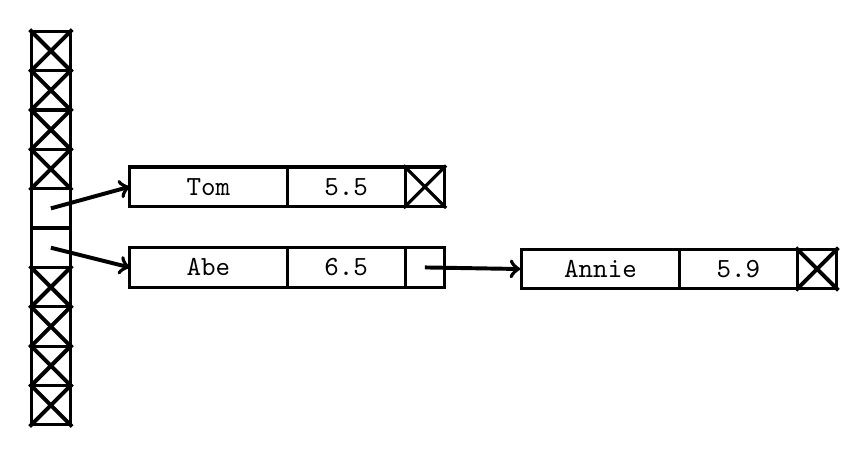
\begin{tikzpicture}
\draw[line width=0.05cm,black] (1.98,0.020000000000000018) to  (2.52,-0.52);
\draw[line width=0.05cm,black] (2.52,0.020000000000000018) to  (1.98,-0.52);
\draw[line width=0.05cm,black] (1.98,-0.48) to  (2.52,-1.02);
\draw[line width=0.05cm,black] (2.52,-0.48) to  (1.98,-1.02);
\draw[line width=0.05cm,black] (1.98,-0.98) to  (2.52,-1.52);
\draw[line width=0.05cm,black] (2.52,-0.98) to  (1.98,-1.52);
\draw[line width=0.05cm,black] (1.98,-1.48) to  (2.52,-2.02);
\draw[line width=0.05cm,black] (2.52,-1.48) to  (1.98,-2.02);

\draw (4.25, -1.975)
  node[draw, line width=0.04cm, , color=black,
       rounded corners=0cm, inner sep=0cm] {

\begin{minipage}[t][0.5cm]{2.0cm}
\mbox{}

\end{minipage}

};\draw (4.25, -1.975) node[color=black] {\texttt{Tom}};
\draw (6.0, -1.975)
  node[draw, line width=0.04cm, , color=black,
       rounded corners=0cm, inner sep=0cm] {

\begin{minipage}[t][0.5cm]{1.5cm}
\mbox{}

\end{minipage}

};\draw (6.0, -1.975) node[color=black] {\texttt{5.5}};
\draw (7.0, -1.975)
  node[draw, line width=0.04cm, , color=black,
       rounded corners=0cm, inner sep=0cm] {

\begin{minipage}[t][0.5cm]{0.5cm}
\mbox{}

\end{minipage}

};\draw[line width=0.05cm,black,->] (2.25,-2.25) to  (3.25,-1.9749999999999999);

\fill[black] (2.25, -2.25) circle (0);
\draw[black] (2.25, -2.25) circle (0.0);\draw[line width=0.04cm,black] (6.73,-1.705) to  (7.27,-2.245);
\draw[line width=0.04cm,black] (7.27,-1.705) to  (6.73,-2.245);

\draw (4.25, -3.0)
  node[draw, line width=0.04cm, , color=black,
       rounded corners=0cm, inner sep=0cm] {

\begin{minipage}[t][0.5cm]{2.0cm}
\mbox{}

\end{minipage}

};\draw (4.25, -3.0) node[color=black] {\texttt{Abe}};
\draw (6.0, -3.0)
  node[draw, line width=0.04cm, , color=black,
       rounded corners=0cm, inner sep=0cm] {

\begin{minipage}[t][0.5cm]{1.5cm}
\mbox{}

\end{minipage}

};\draw (6.0, -3.0) node[color=black] {\texttt{6.5}};
\draw (7.0, -3.0)
  node[draw, line width=0.04cm, , color=black,
       rounded corners=0cm, inner sep=0cm] {

\begin{minipage}[t][0.5cm]{0.5cm}
\mbox{}

\end{minipage}

};\draw[line width=0.05cm,black,->] (2.25,-2.75) to  (3.25,-3.0);

\fill[black] (2.25, -2.75) circle (0);
\draw[black] (2.25, -2.75) circle (0.0);
\draw (9.23, -3.02)
  node[draw, line width=0.04cm, , color=black,
       rounded corners=0cm, inner sep=0cm] {

\begin{minipage}[t][0.5cm]{2.0cm}
\mbox{}

\end{minipage}

};\draw (9.23, -3.02) node[color=black] {\texttt{Annie}};
\draw (10.98, -3.02)
  node[draw, line width=0.04cm, , color=black,
       rounded corners=0cm, inner sep=0cm] {

\begin{minipage}[t][0.5cm]{1.5cm}
\mbox{}

\end{minipage}

};\draw (10.98, -3.02) node[color=black] {\texttt{5.9}};
\draw (11.98, -3.02)
  node[draw, line width=0.04cm, , color=black,
       rounded corners=0cm, inner sep=0cm] {

\begin{minipage}[t][0.5cm]{0.5cm}
\mbox{}

\end{minipage}

};\draw[line width=0.05cm,black] (11.71,-2.75) to  (12.25,-3.29);
\draw[line width=0.05cm,black] (12.25,-2.75) to  (11.71,-3.29);
\draw[line width=0.05cm,black,->] (7.0,-3.0) to  (8.21,-3.0199999999999996);

\fill[black] (7.0, -3.0) circle (0);
\draw[black] (7.0, -3.0) circle (0.0);\draw[line width=0.05cm,black] (1.98,-2.98) to  (2.52,-3.52);
\draw[line width=0.05cm,black] (2.52,-2.98) to  (1.98,-3.52);
\draw[line width=0.05cm,black] (1.98,-3.4800000000000004) to  (2.52,-4.02);
\draw[line width=0.05cm,black] (2.52,-3.4800000000000004) to  (1.98,-4.02);
\draw[line width=0.05cm,black] (1.98,-3.9800000000000004) to  (2.52,-4.52);
\draw[line width=0.05cm,black] (2.52,-3.9800000000000004) to  (1.98,-4.52);
\draw[line width=0.05cm,black] (1.98,-4.48) to  (2.52,-5.02);
\draw[line width=0.05cm,black] (2.52,-4.48) to  (1.98,-5.02);

\draw (2.25, -0.25)
  node[draw, line width=0.04cm, , color=black,
       rounded corners=0cm, inner sep=0cm] {

\begin{minipage}[t][0.5cm]{0.5cm}
\mbox{}

\end{minipage}

};
\draw (2.25, -0.75)
  node[draw, line width=0.04cm, , color=black,
       rounded corners=0cm, inner sep=0cm] {

\begin{minipage}[t][0.5cm]{0.5cm}
\mbox{}

\end{minipage}

};
\draw (2.25, -1.25)
  node[draw, line width=0.04cm, , color=black,
       rounded corners=0cm, inner sep=0cm] {

\begin{minipage}[t][0.5cm]{0.5cm}
\mbox{}

\end{minipage}

};
\draw (2.25, -1.75)
  node[draw, line width=0.04cm, , color=black,
       rounded corners=0cm, inner sep=0cm] {

\begin{minipage}[t][0.5cm]{0.5cm}
\mbox{}

\end{minipage}

};
\draw (2.25, -2.25)
  node[draw, line width=0.04cm, , color=black,
       rounded corners=0cm, inner sep=0cm] {

\begin{minipage}[t][0.5cm]{0.5cm}
\mbox{}

\end{minipage}

};
\draw (2.25, -2.75)
  node[draw, line width=0.04cm, , color=black,
       rounded corners=0cm, inner sep=0cm] {

\begin{minipage}[t][0.5cm]{0.5cm}
\mbox{}

\end{minipage}

};
\draw (2.25, -3.25)
  node[draw, line width=0.04cm, , color=black,
       rounded corners=0cm, inner sep=0cm] {

\begin{minipage}[t][0.5cm]{0.5cm}
\mbox{}

\end{minipage}

};
\draw (2.25, -3.75)
  node[draw, line width=0.04cm, , color=black,
       rounded corners=0cm, inner sep=0cm] {

\begin{minipage}[t][0.5cm]{0.5cm}
\mbox{}

\end{minipage}

};
\draw (2.25, -4.25)
  node[draw, line width=0.04cm, , color=black,
       rounded corners=0cm, inner sep=0cm] {

\begin{minipage}[t][0.5cm]{0.5cm}
\mbox{}

\end{minipage}

};
\draw (2.25, -4.75)
  node[draw, line width=0.04cm, , color=black,
       rounded corners=0cm, inner sep=0cm] {

\begin{minipage}[t][0.5cm]{0.5cm}
\mbox{}

\end{minipage}

};
\end{tikzpicture}

\end{center}



This is the usual node removal operation for a \textit{general} tree.

I want to add another node remove operation:
Suppose the node to be removed has only \textit{one} child,
then there's an obvious way to remove the node.
For instance look at

\begin{center}
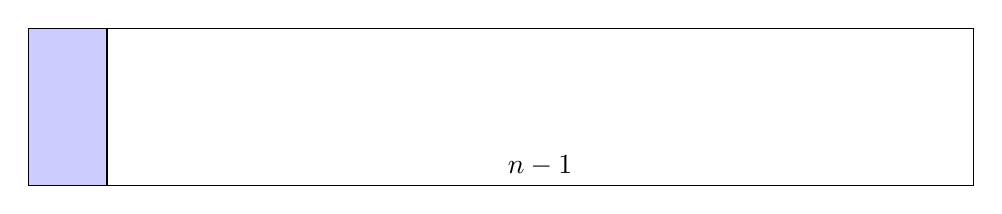
\begin{tikzpicture}

\draw (6.0, 1.0)
  node[draw, , , color=black,
       rounded corners=0cm, inner sep=0cm] {

\begin{minipage}[t][2cm]{12cm}
\mbox{}

\end{minipage}

};
\draw (0.5, 1.0)
  node[fill=blue!20!white,rounded corners=0cm,inner sep=0cm] {

\begin{minipage}[t][2cm]{1cm}
\mbox{}

\end{minipage}

};
\draw (0.5, 1.0)
  node[draw, , , color=black,
       rounded corners=0cm, inner sep=0cm] {

\begin{minipage}[t][2cm]{1cm}
\mbox{}

\end{minipage}

};
\draw (6.5, 0.25)
  node[draw=none, line width=0cm, , color=black,
       rounded corners=0cm, inner sep=0cm] {

\begin{minipage}[t][0.1cm]{0.1cm}
\mbox{}

\end{minipage}

};\draw (6.5, 0.25) node[color=black] {$n - 1$};
\end{tikzpicture}

\end{center}



On removing $h$, we get

\begin{center}
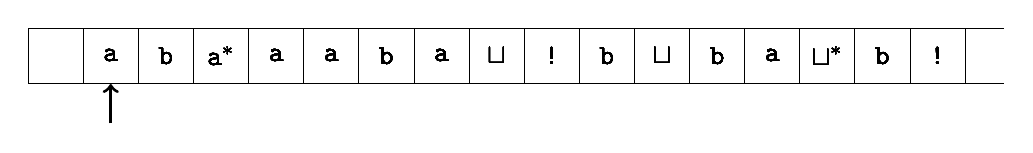
\begin{tikzpicture}

\draw (0.35, 0.35)
  node[draw, line width=0.01cm, , color=black,
       rounded corners=0cm, inner sep=0cm] {

\begin{minipage}[t][0.7cm]{0.7cm}
\mbox{}

\end{minipage}

};\draw (0.35, 0.35) node[color=black] {\texttt{\DOLLAR}};
\draw (1.0499999999999998, 0.35)
  node[draw, line width=0.01cm, , color=black,
       rounded corners=0cm, inner sep=0cm] {

\begin{minipage}[t][0.7cm]{0.7cm}
\mbox{}

\end{minipage}

};\draw (1.0499999999999998, 0.35) node[color=black] {\texttt{a}};
\draw (1.7499999999999998, 0.35)
  node[draw, line width=0.01cm, , color=black,
       rounded corners=0cm, inner sep=0cm] {

\begin{minipage}[t][0.7cm]{0.7cm}
\mbox{}

\end{minipage}

};\draw (1.7499999999999998, 0.35) node[color=black] {\texttt{b}};
\draw (2.4499999999999997, 0.35)
  node[draw, line width=0.01cm, , color=black,
       rounded corners=0cm, inner sep=0cm] {

\begin{minipage}[t][0.7cm]{0.7cm}
\mbox{}

\end{minipage}

};\draw (2.4499999999999997, 0.35) node[color=black] {\texttt{a$^*$}};
\draw (3.15, 0.35)
  node[draw, line width=0.01cm, , color=black,
       rounded corners=0cm, inner sep=0cm] {

\begin{minipage}[t][0.7cm]{0.7cm}
\mbox{}

\end{minipage}

};\draw (3.15, 0.35) node[color=black] {\texttt{a}};
\draw (3.85, 0.35)
  node[draw, line width=0.01cm, , color=black,
       rounded corners=0cm, inner sep=0cm] {

\begin{minipage}[t][0.7cm]{0.7cm}
\mbox{}

\end{minipage}

};\draw (3.85, 0.35) node[color=black] {\texttt{a}};
\draw (4.550000000000001, 0.35)
  node[draw, line width=0.01cm, , color=black,
       rounded corners=0cm, inner sep=0cm] {

\begin{minipage}[t][0.7cm]{0.7cm}
\mbox{}

\end{minipage}

};\draw (4.550000000000001, 0.35) node[color=black] {\texttt{b}};
\draw (5.25, 0.35)
  node[draw, line width=0.01cm, , color=black,
       rounded corners=0cm, inner sep=0cm] {

\begin{minipage}[t][0.7cm]{0.7cm}
\mbox{}

\end{minipage}

};\draw (5.25, 0.35) node[color=black] {\texttt{a}};
\draw (5.950000000000001, 0.35)
  node[draw, line width=0.01cm, , color=black,
       rounded corners=0cm, inner sep=0cm] {

\begin{minipage}[t][0.7cm]{0.7cm}
\mbox{}

\end{minipage}

};\draw (5.950000000000001, 0.35) node[color=black] {\texttt{$\sqcup$}};
\draw (6.65, 0.35)
  node[draw, line width=0.01cm, , color=black,
       rounded corners=0cm, inner sep=0cm] {

\begin{minipage}[t][0.7cm]{0.7cm}
\mbox{}

\end{minipage}

};\draw (6.65, 0.35) node[color=black] {\texttt{!}};
\draw (7.350000000000001, 0.35)
  node[draw, line width=0.01cm, , color=black,
       rounded corners=0cm, inner sep=0cm] {

\begin{minipage}[t][0.7cm]{0.7cm}
\mbox{}

\end{minipage}

};\draw (7.350000000000001, 0.35) node[color=black] {\texttt{b}};
\draw (8.05, 0.35)
  node[draw, line width=0.01cm, , color=black,
       rounded corners=0cm, inner sep=0cm] {

\begin{minipage}[t][0.7cm]{0.7cm}
\mbox{}

\end{minipage}

};\draw (8.05, 0.35) node[color=black] {\texttt{$\sqcup$}};
\draw (8.75, 0.35)
  node[draw, line width=0.01cm, , color=black,
       rounded corners=0cm, inner sep=0cm] {

\begin{minipage}[t][0.7cm]{0.7cm}
\mbox{}

\end{minipage}

};\draw (8.75, 0.35) node[color=black] {\texttt{b}};
\draw (9.45, 0.35)
  node[draw, line width=0.01cm, , color=black,
       rounded corners=0cm, inner sep=0cm] {

\begin{minipage}[t][0.7cm]{0.7cm}
\mbox{}

\end{minipage}

};\draw (9.45, 0.35) node[color=black] {\texttt{a}};
\draw (10.149999999999999, 0.35)
  node[draw, line width=0.01cm, , color=black,
       rounded corners=0cm, inner sep=0cm] {

\begin{minipage}[t][0.7cm]{0.7cm}
\mbox{}

\end{minipage}

};\draw (10.149999999999999, 0.35) node[color=black] {\texttt{$\sqcup^*$}};
\draw (10.849999999999998, 0.35)
  node[draw, line width=0.01cm, , color=black,
       rounded corners=0cm, inner sep=0cm] {

\begin{minipage}[t][0.7cm]{0.7cm}
\mbox{}

\end{minipage}

};\draw (10.849999999999998, 0.35) node[color=black] {\texttt{b}};
\draw (11.549999999999997, 0.35)
  node[draw, line width=0.01cm, , color=black,
       rounded corners=0cm, inner sep=0cm] {

\begin{minipage}[t][0.7cm]{0.7cm}
\mbox{}

\end{minipage}

};\draw (11.549999999999997, 0.35) node[color=black] {\texttt{!}};
\draw (0.35, 0.35)
  node[draw, line width=0.01cm, , color=black,
       rounded corners=0cm, inner sep=0cm] {

\begin{minipage}[t][0.7cm]{0.7cm}
\mbox{}

\end{minipage}

};\draw (0.35, 0.35) node[color=black] {\texttt{\DOLLAR}};
\draw (1.0499999999999998, 0.35)
  node[draw, line width=0.01cm, , color=black,
       rounded corners=0cm, inner sep=0cm] {

\begin{minipage}[t][0.7cm]{0.7cm}
\mbox{}

\end{minipage}

};\draw (1.0499999999999998, 0.35) node[color=black] {\texttt{a}};
\draw (1.7499999999999998, 0.35)
  node[draw, line width=0.01cm, , color=black,
       rounded corners=0cm, inner sep=0cm] {

\begin{minipage}[t][0.7cm]{0.7cm}
\mbox{}

\end{minipage}

};\draw (1.7499999999999998, 0.35) node[color=black] {\texttt{b}};
\draw (2.4499999999999997, 0.35)
  node[draw, line width=0.01cm, , color=black,
       rounded corners=0cm, inner sep=0cm] {

\begin{minipage}[t][0.7cm]{0.7cm}
\mbox{}

\end{minipage}

};\draw (2.4499999999999997, 0.35) node[color=black] {\texttt{a$^*$}};
\draw (3.15, 0.35)
  node[draw, line width=0.01cm, , color=black,
       rounded corners=0cm, inner sep=0cm] {

\begin{minipage}[t][0.7cm]{0.7cm}
\mbox{}

\end{minipage}

};\draw (3.15, 0.35) node[color=black] {\texttt{a}};
\draw (3.85, 0.35)
  node[draw, line width=0.01cm, , color=black,
       rounded corners=0cm, inner sep=0cm] {

\begin{minipage}[t][0.7cm]{0.7cm}
\mbox{}

\end{minipage}

};\draw (3.85, 0.35) node[color=black] {\texttt{a}};
\draw (4.550000000000001, 0.35)
  node[draw, line width=0.01cm, , color=black,
       rounded corners=0cm, inner sep=0cm] {

\begin{minipage}[t][0.7cm]{0.7cm}
\mbox{}

\end{minipage}

};\draw (4.550000000000001, 0.35) node[color=black] {\texttt{b}};
\draw (5.25, 0.35)
  node[draw, line width=0.01cm, , color=black,
       rounded corners=0cm, inner sep=0cm] {

\begin{minipage}[t][0.7cm]{0.7cm}
\mbox{}

\end{minipage}

};\draw (5.25, 0.35) node[color=black] {\texttt{a}};
\draw (5.950000000000001, 0.35)
  node[draw, line width=0.01cm, , color=black,
       rounded corners=0cm, inner sep=0cm] {

\begin{minipage}[t][0.7cm]{0.7cm}
\mbox{}

\end{minipage}

};\draw (5.950000000000001, 0.35) node[color=black] {\texttt{$\sqcup$}};
\draw (6.65, 0.35)
  node[draw, line width=0.01cm, , color=black,
       rounded corners=0cm, inner sep=0cm] {

\begin{minipage}[t][0.7cm]{0.7cm}
\mbox{}

\end{minipage}

};\draw (6.65, 0.35) node[color=black] {\texttt{!}};
\draw (7.350000000000001, 0.35)
  node[draw, line width=0.01cm, , color=black,
       rounded corners=0cm, inner sep=0cm] {

\begin{minipage}[t][0.7cm]{0.7cm}
\mbox{}

\end{minipage}

};\draw (7.350000000000001, 0.35) node[color=black] {\texttt{b}};
\draw (8.05, 0.35)
  node[draw, line width=0.01cm, , color=black,
       rounded corners=0cm, inner sep=0cm] {

\begin{minipage}[t][0.7cm]{0.7cm}
\mbox{}

\end{minipage}

};\draw (8.05, 0.35) node[color=black] {\texttt{$\sqcup$}};
\draw (8.75, 0.35)
  node[draw, line width=0.01cm, , color=black,
       rounded corners=0cm, inner sep=0cm] {

\begin{minipage}[t][0.7cm]{0.7cm}
\mbox{}

\end{minipage}

};\draw (8.75, 0.35) node[color=black] {\texttt{b}};
\draw (9.45, 0.35)
  node[draw, line width=0.01cm, , color=black,
       rounded corners=0cm, inner sep=0cm] {

\begin{minipage}[t][0.7cm]{0.7cm}
\mbox{}

\end{minipage}

};\draw (9.45, 0.35) node[color=black] {\texttt{a}};
\draw (10.149999999999999, 0.35)
  node[draw, line width=0.01cm, , color=black,
       rounded corners=0cm, inner sep=0cm] {

\begin{minipage}[t][0.7cm]{0.7cm}
\mbox{}

\end{minipage}

};\draw (10.149999999999999, 0.35) node[color=black] {\texttt{$\sqcup^*$}};
\draw (10.849999999999998, 0.35)
  node[draw, line width=0.01cm, , color=black,
       rounded corners=0cm, inner sep=0cm] {

\begin{minipage}[t][0.7cm]{0.7cm}
\mbox{}

\end{minipage}

};\draw (10.849999999999998, 0.35) node[color=black] {\texttt{b}};
\draw (11.549999999999997, 0.35)
  node[draw, line width=0.01cm, , color=black,
       rounded corners=0cm, inner sep=0cm] {

\begin{minipage}[t][0.7cm]{0.7cm}
\mbox{}

\end{minipage}

};\draw (11.549999999999997, 0.35) node[color=black] {\texttt{!}};
\draw (0.35, 0.35)
  node[draw, line width=0.01cm, , color=black,
       rounded corners=0cm, inner sep=0cm] {

\begin{minipage}[t][0.7cm]{0.7cm}
\mbox{}

\end{minipage}

};\draw (0.35, 0.35) node[color=black] {\texttt{\DOLLAR}};
\draw (1.0499999999999998, 0.35)
  node[draw, line width=0.01cm, , color=black,
       rounded corners=0cm, inner sep=0cm] {

\begin{minipage}[t][0.7cm]{0.7cm}
\mbox{}

\end{minipage}

};\draw (1.0499999999999998, 0.35) node[color=black] {\texttt{a}};
\draw (1.7499999999999998, 0.35)
  node[draw, line width=0.01cm, , color=black,
       rounded corners=0cm, inner sep=0cm] {

\begin{minipage}[t][0.7cm]{0.7cm}
\mbox{}

\end{minipage}

};\draw (1.7499999999999998, 0.35) node[color=black] {\texttt{b}};
\draw (2.4499999999999997, 0.35)
  node[draw, line width=0.01cm, , color=black,
       rounded corners=0cm, inner sep=0cm] {

\begin{minipage}[t][0.7cm]{0.7cm}
\mbox{}

\end{minipage}

};\draw (2.4499999999999997, 0.35) node[color=black] {\texttt{a$^*$}};
\draw (3.15, 0.35)
  node[draw, line width=0.01cm, , color=black,
       rounded corners=0cm, inner sep=0cm] {

\begin{minipage}[t][0.7cm]{0.7cm}
\mbox{}

\end{minipage}

};\draw (3.15, 0.35) node[color=black] {\texttt{a}};
\draw (3.85, 0.35)
  node[draw, line width=0.01cm, , color=black,
       rounded corners=0cm, inner sep=0cm] {

\begin{minipage}[t][0.7cm]{0.7cm}
\mbox{}

\end{minipage}

};\draw (3.85, 0.35) node[color=black] {\texttt{a}};
\draw (4.550000000000001, 0.35)
  node[draw, line width=0.01cm, , color=black,
       rounded corners=0cm, inner sep=0cm] {

\begin{minipage}[t][0.7cm]{0.7cm}
\mbox{}

\end{minipage}

};\draw (4.550000000000001, 0.35) node[color=black] {\texttt{b}};
\draw (5.25, 0.35)
  node[draw, line width=0.01cm, , color=black,
       rounded corners=0cm, inner sep=0cm] {

\begin{minipage}[t][0.7cm]{0.7cm}
\mbox{}

\end{minipage}

};\draw (5.25, 0.35) node[color=black] {\texttt{a}};
\draw (5.950000000000001, 0.35)
  node[draw, line width=0.01cm, , color=black,
       rounded corners=0cm, inner sep=0cm] {

\begin{minipage}[t][0.7cm]{0.7cm}
\mbox{}

\end{minipage}

};\draw (5.950000000000001, 0.35) node[color=black] {\texttt{$\sqcup$}};
\draw (6.65, 0.35)
  node[draw, line width=0.01cm, , color=black,
       rounded corners=0cm, inner sep=0cm] {

\begin{minipage}[t][0.7cm]{0.7cm}
\mbox{}

\end{minipage}

};\draw (6.65, 0.35) node[color=black] {\texttt{!}};
\draw (7.350000000000001, 0.35)
  node[draw, line width=0.01cm, , color=black,
       rounded corners=0cm, inner sep=0cm] {

\begin{minipage}[t][0.7cm]{0.7cm}
\mbox{}

\end{minipage}

};\draw (7.350000000000001, 0.35) node[color=black] {\texttt{b}};
\draw (8.05, 0.35)
  node[draw, line width=0.01cm, , color=black,
       rounded corners=0cm, inner sep=0cm] {

\begin{minipage}[t][0.7cm]{0.7cm}
\mbox{}

\end{minipage}

};\draw (8.05, 0.35) node[color=black] {\texttt{$\sqcup$}};
\draw (8.75, 0.35)
  node[draw, line width=0.01cm, , color=black,
       rounded corners=0cm, inner sep=0cm] {

\begin{minipage}[t][0.7cm]{0.7cm}
\mbox{}

\end{minipage}

};\draw (8.75, 0.35) node[color=black] {\texttt{b}};
\draw (9.45, 0.35)
  node[draw, line width=0.01cm, , color=black,
       rounded corners=0cm, inner sep=0cm] {

\begin{minipage}[t][0.7cm]{0.7cm}
\mbox{}

\end{minipage}

};\draw (9.45, 0.35) node[color=black] {\texttt{a}};
\draw (10.149999999999999, 0.35)
  node[draw, line width=0.01cm, , color=black,
       rounded corners=0cm, inner sep=0cm] {

\begin{minipage}[t][0.7cm]{0.7cm}
\mbox{}

\end{minipage}

};\draw (10.149999999999999, 0.35) node[color=black] {\texttt{$\sqcup^*$}};
\draw (10.849999999999998, 0.35)
  node[draw, line width=0.01cm, , color=black,
       rounded corners=0cm, inner sep=0cm] {

\begin{minipage}[t][0.7cm]{0.7cm}
\mbox{}

\end{minipage}

};\draw (10.849999999999998, 0.35) node[color=black] {\texttt{b}};
\draw (11.549999999999997, 0.35)
  node[draw, line width=0.01cm, , color=black,
       rounded corners=0cm, inner sep=0cm] {

\begin{minipage}[t][0.7cm]{0.7cm}
\mbox{}

\end{minipage}

};\draw (11.549999999999997, 0.35) node[color=black] {\texttt{!}};
\draw (0.35, 0.35)
  node[draw, line width=0.01cm, , color=black,
       rounded corners=0cm, inner sep=0cm] {

\begin{minipage}[t][0.7cm]{0.7cm}
\mbox{}

\end{minipage}

};\draw (0.35, 0.35) node[color=black] {\texttt{\DOLLAR}};
\draw (1.0499999999999998, 0.35)
  node[draw, line width=0.01cm, , color=black,
       rounded corners=0cm, inner sep=0cm] {

\begin{minipage}[t][0.7cm]{0.7cm}
\mbox{}

\end{minipage}

};\draw (1.0499999999999998, 0.35) node[color=black] {\texttt{a}};
\draw (1.7499999999999998, 0.35)
  node[draw, line width=0.01cm, , color=black,
       rounded corners=0cm, inner sep=0cm] {

\begin{minipage}[t][0.7cm]{0.7cm}
\mbox{}

\end{minipage}

};\draw (1.7499999999999998, 0.35) node[color=black] {\texttt{b}};
\draw (2.4499999999999997, 0.35)
  node[draw, line width=0.01cm, , color=black,
       rounded corners=0cm, inner sep=0cm] {

\begin{minipage}[t][0.7cm]{0.7cm}
\mbox{}

\end{minipage}

};\draw (2.4499999999999997, 0.35) node[color=black] {\texttt{a$^*$}};
\draw (3.15, 0.35)
  node[draw, line width=0.01cm, , color=black,
       rounded corners=0cm, inner sep=0cm] {

\begin{minipage}[t][0.7cm]{0.7cm}
\mbox{}

\end{minipage}

};\draw (3.15, 0.35) node[color=black] {\texttt{a}};
\draw (3.85, 0.35)
  node[draw, line width=0.01cm, , color=black,
       rounded corners=0cm, inner sep=0cm] {

\begin{minipage}[t][0.7cm]{0.7cm}
\mbox{}

\end{minipage}

};\draw (3.85, 0.35) node[color=black] {\texttt{a}};
\draw (4.550000000000001, 0.35)
  node[draw, line width=0.01cm, , color=black,
       rounded corners=0cm, inner sep=0cm] {

\begin{minipage}[t][0.7cm]{0.7cm}
\mbox{}

\end{minipage}

};\draw (4.550000000000001, 0.35) node[color=black] {\texttt{b}};
\draw (5.25, 0.35)
  node[draw, line width=0.01cm, , color=black,
       rounded corners=0cm, inner sep=0cm] {

\begin{minipage}[t][0.7cm]{0.7cm}
\mbox{}

\end{minipage}

};\draw (5.25, 0.35) node[color=black] {\texttt{a}};
\draw (5.950000000000001, 0.35)
  node[draw, line width=0.01cm, , color=black,
       rounded corners=0cm, inner sep=0cm] {

\begin{minipage}[t][0.7cm]{0.7cm}
\mbox{}

\end{minipage}

};\draw (5.950000000000001, 0.35) node[color=black] {\texttt{$\sqcup$}};
\draw (6.65, 0.35)
  node[draw, line width=0.01cm, , color=black,
       rounded corners=0cm, inner sep=0cm] {

\begin{minipage}[t][0.7cm]{0.7cm}
\mbox{}

\end{minipage}

};\draw (6.65, 0.35) node[color=black] {\texttt{!}};
\draw (7.350000000000001, 0.35)
  node[draw, line width=0.01cm, , color=black,
       rounded corners=0cm, inner sep=0cm] {

\begin{minipage}[t][0.7cm]{0.7cm}
\mbox{}

\end{minipage}

};\draw (7.350000000000001, 0.35) node[color=black] {\texttt{b}};
\draw (8.05, 0.35)
  node[draw, line width=0.01cm, , color=black,
       rounded corners=0cm, inner sep=0cm] {

\begin{minipage}[t][0.7cm]{0.7cm}
\mbox{}

\end{minipage}

};\draw (8.05, 0.35) node[color=black] {\texttt{$\sqcup$}};
\draw (8.75, 0.35)
  node[draw, line width=0.01cm, , color=black,
       rounded corners=0cm, inner sep=0cm] {

\begin{minipage}[t][0.7cm]{0.7cm}
\mbox{}

\end{minipage}

};\draw (8.75, 0.35) node[color=black] {\texttt{b}};
\draw (9.45, 0.35)
  node[draw, line width=0.01cm, , color=black,
       rounded corners=0cm, inner sep=0cm] {

\begin{minipage}[t][0.7cm]{0.7cm}
\mbox{}

\end{minipage}

};\draw (9.45, 0.35) node[color=black] {\texttt{a}};
\draw (10.149999999999999, 0.35)
  node[draw, line width=0.01cm, , color=black,
       rounded corners=0cm, inner sep=0cm] {

\begin{minipage}[t][0.7cm]{0.7cm}
\mbox{}

\end{minipage}

};\draw (10.149999999999999, 0.35) node[color=black] {\texttt{$\sqcup^*$}};
\draw (10.849999999999998, 0.35)
  node[draw, line width=0.01cm, , color=black,
       rounded corners=0cm, inner sep=0cm] {

\begin{minipage}[t][0.7cm]{0.7cm}
\mbox{}

\end{minipage}

};\draw (10.849999999999998, 0.35) node[color=black] {\texttt{b}};
\draw (11.549999999999997, 0.35)
  node[draw, line width=0.01cm, , color=black,
       rounded corners=0cm, inner sep=0cm] {

\begin{minipage}[t][0.7cm]{0.7cm}
\mbox{}

\end{minipage}

};\draw (11.549999999999997, 0.35) node[color=black] {\texttt{!}};
\draw (0.35, 0.35)
  node[draw, line width=0.01cm, , color=black,
       rounded corners=0cm, inner sep=0cm] {

\begin{minipage}[t][0.7cm]{0.7cm}
\mbox{}

\end{minipage}

};\draw (0.35, 0.35) node[color=black] {\texttt{\DOLLAR}};
\draw (1.0499999999999998, 0.35)
  node[draw, line width=0.01cm, , color=black,
       rounded corners=0cm, inner sep=0cm] {

\begin{minipage}[t][0.7cm]{0.7cm}
\mbox{}

\end{minipage}

};\draw (1.0499999999999998, 0.35) node[color=black] {\texttt{a}};
\draw (1.7499999999999998, 0.35)
  node[draw, line width=0.01cm, , color=black,
       rounded corners=0cm, inner sep=0cm] {

\begin{minipage}[t][0.7cm]{0.7cm}
\mbox{}

\end{minipage}

};\draw (1.7499999999999998, 0.35) node[color=black] {\texttt{b}};
\draw (2.4499999999999997, 0.35)
  node[draw, line width=0.01cm, , color=black,
       rounded corners=0cm, inner sep=0cm] {

\begin{minipage}[t][0.7cm]{0.7cm}
\mbox{}

\end{minipage}

};\draw (2.4499999999999997, 0.35) node[color=black] {\texttt{a$^*$}};
\draw (3.15, 0.35)
  node[draw, line width=0.01cm, , color=black,
       rounded corners=0cm, inner sep=0cm] {

\begin{minipage}[t][0.7cm]{0.7cm}
\mbox{}

\end{minipage}

};\draw (3.15, 0.35) node[color=black] {\texttt{a}};
\draw (3.85, 0.35)
  node[draw, line width=0.01cm, , color=black,
       rounded corners=0cm, inner sep=0cm] {

\begin{minipage}[t][0.7cm]{0.7cm}
\mbox{}

\end{minipage}

};\draw (3.85, 0.35) node[color=black] {\texttt{a}};
\draw (4.550000000000001, 0.35)
  node[draw, line width=0.01cm, , color=black,
       rounded corners=0cm, inner sep=0cm] {

\begin{minipage}[t][0.7cm]{0.7cm}
\mbox{}

\end{minipage}

};\draw (4.550000000000001, 0.35) node[color=black] {\texttt{b}};
\draw (5.25, 0.35)
  node[draw, line width=0.01cm, , color=black,
       rounded corners=0cm, inner sep=0cm] {

\begin{minipage}[t][0.7cm]{0.7cm}
\mbox{}

\end{minipage}

};\draw (5.25, 0.35) node[color=black] {\texttt{a}};
\draw (5.950000000000001, 0.35)
  node[draw, line width=0.01cm, , color=black,
       rounded corners=0cm, inner sep=0cm] {

\begin{minipage}[t][0.7cm]{0.7cm}
\mbox{}

\end{minipage}

};\draw (5.950000000000001, 0.35) node[color=black] {\texttt{$\sqcup$}};
\draw (6.65, 0.35)
  node[draw, line width=0.01cm, , color=black,
       rounded corners=0cm, inner sep=0cm] {

\begin{minipage}[t][0.7cm]{0.7cm}
\mbox{}

\end{minipage}

};\draw (6.65, 0.35) node[color=black] {\texttt{!}};
\draw (7.350000000000001, 0.35)
  node[draw, line width=0.01cm, , color=black,
       rounded corners=0cm, inner sep=0cm] {

\begin{minipage}[t][0.7cm]{0.7cm}
\mbox{}

\end{minipage}

};\draw (7.350000000000001, 0.35) node[color=black] {\texttt{b}};
\draw (8.05, 0.35)
  node[draw, line width=0.01cm, , color=black,
       rounded corners=0cm, inner sep=0cm] {

\begin{minipage}[t][0.7cm]{0.7cm}
\mbox{}

\end{minipage}

};\draw (8.05, 0.35) node[color=black] {\texttt{$\sqcup$}};
\draw (8.75, 0.35)
  node[draw, line width=0.01cm, , color=black,
       rounded corners=0cm, inner sep=0cm] {

\begin{minipage}[t][0.7cm]{0.7cm}
\mbox{}

\end{minipage}

};\draw (8.75, 0.35) node[color=black] {\texttt{b}};
\draw (9.45, 0.35)
  node[draw, line width=0.01cm, , color=black,
       rounded corners=0cm, inner sep=0cm] {

\begin{minipage}[t][0.7cm]{0.7cm}
\mbox{}

\end{minipage}

};\draw (9.45, 0.35) node[color=black] {\texttt{a}};
\draw (10.149999999999999, 0.35)
  node[draw, line width=0.01cm, , color=black,
       rounded corners=0cm, inner sep=0cm] {

\begin{minipage}[t][0.7cm]{0.7cm}
\mbox{}

\end{minipage}

};\draw (10.149999999999999, 0.35) node[color=black] {\texttt{$\sqcup^*$}};
\draw (10.849999999999998, 0.35)
  node[draw, line width=0.01cm, , color=black,
       rounded corners=0cm, inner sep=0cm] {

\begin{minipage}[t][0.7cm]{0.7cm}
\mbox{}

\end{minipage}

};\draw (10.849999999999998, 0.35) node[color=black] {\texttt{b}};
\draw (11.549999999999997, 0.35)
  node[draw, line width=0.01cm, , color=black,
       rounded corners=0cm, inner sep=0cm] {

\begin{minipage}[t][0.7cm]{0.7cm}
\mbox{}

\end{minipage}

};\draw (11.549999999999997, 0.35) node[color=black] {\texttt{!}};
\draw (0.35, 0.35)
  node[draw, line width=0.01cm, , color=black,
       rounded corners=0cm, inner sep=0cm] {

\begin{minipage}[t][0.7cm]{0.7cm}
\mbox{}

\end{minipage}

};\draw (0.35, 0.35) node[color=black] {\texttt{\DOLLAR}};
\draw (1.0499999999999998, 0.35)
  node[draw, line width=0.01cm, , color=black,
       rounded corners=0cm, inner sep=0cm] {

\begin{minipage}[t][0.7cm]{0.7cm}
\mbox{}

\end{minipage}

};\draw (1.0499999999999998, 0.35) node[color=black] {\texttt{a}};
\draw (1.7499999999999998, 0.35)
  node[draw, line width=0.01cm, , color=black,
       rounded corners=0cm, inner sep=0cm] {

\begin{minipage}[t][0.7cm]{0.7cm}
\mbox{}

\end{minipage}

};\draw (1.7499999999999998, 0.35) node[color=black] {\texttt{b}};
\draw (2.4499999999999997, 0.35)
  node[draw, line width=0.01cm, , color=black,
       rounded corners=0cm, inner sep=0cm] {

\begin{minipage}[t][0.7cm]{0.7cm}
\mbox{}

\end{minipage}

};\draw (2.4499999999999997, 0.35) node[color=black] {\texttt{a$^*$}};
\draw (3.15, 0.35)
  node[draw, line width=0.01cm, , color=black,
       rounded corners=0cm, inner sep=0cm] {

\begin{minipage}[t][0.7cm]{0.7cm}
\mbox{}

\end{minipage}

};\draw (3.15, 0.35) node[color=black] {\texttt{a}};
\draw (3.85, 0.35)
  node[draw, line width=0.01cm, , color=black,
       rounded corners=0cm, inner sep=0cm] {

\begin{minipage}[t][0.7cm]{0.7cm}
\mbox{}

\end{minipage}

};\draw (3.85, 0.35) node[color=black] {\texttt{a}};
\draw (4.550000000000001, 0.35)
  node[draw, line width=0.01cm, , color=black,
       rounded corners=0cm, inner sep=0cm] {

\begin{minipage}[t][0.7cm]{0.7cm}
\mbox{}

\end{minipage}

};\draw (4.550000000000001, 0.35) node[color=black] {\texttt{b}};
\draw (5.25, 0.35)
  node[draw, line width=0.01cm, , color=black,
       rounded corners=0cm, inner sep=0cm] {

\begin{minipage}[t][0.7cm]{0.7cm}
\mbox{}

\end{minipage}

};\draw (5.25, 0.35) node[color=black] {\texttt{a}};
\draw (5.950000000000001, 0.35)
  node[draw, line width=0.01cm, , color=black,
       rounded corners=0cm, inner sep=0cm] {

\begin{minipage}[t][0.7cm]{0.7cm}
\mbox{}

\end{minipage}

};\draw (5.950000000000001, 0.35) node[color=black] {\texttt{$\sqcup$}};
\draw (6.65, 0.35)
  node[draw, line width=0.01cm, , color=black,
       rounded corners=0cm, inner sep=0cm] {

\begin{minipage}[t][0.7cm]{0.7cm}
\mbox{}

\end{minipage}

};\draw (6.65, 0.35) node[color=black] {\texttt{!}};
\draw (7.350000000000001, 0.35)
  node[draw, line width=0.01cm, , color=black,
       rounded corners=0cm, inner sep=0cm] {

\begin{minipage}[t][0.7cm]{0.7cm}
\mbox{}

\end{minipage}

};\draw (7.350000000000001, 0.35) node[color=black] {\texttt{b}};
\draw (8.05, 0.35)
  node[draw, line width=0.01cm, , color=black,
       rounded corners=0cm, inner sep=0cm] {

\begin{minipage}[t][0.7cm]{0.7cm}
\mbox{}

\end{minipage}

};\draw (8.05, 0.35) node[color=black] {\texttt{$\sqcup$}};
\draw (8.75, 0.35)
  node[draw, line width=0.01cm, , color=black,
       rounded corners=0cm, inner sep=0cm] {

\begin{minipage}[t][0.7cm]{0.7cm}
\mbox{}

\end{minipage}

};\draw (8.75, 0.35) node[color=black] {\texttt{b}};
\draw (9.45, 0.35)
  node[draw, line width=0.01cm, , color=black,
       rounded corners=0cm, inner sep=0cm] {

\begin{minipage}[t][0.7cm]{0.7cm}
\mbox{}

\end{minipage}

};\draw (9.45, 0.35) node[color=black] {\texttt{a}};
\draw (10.149999999999999, 0.35)
  node[draw, line width=0.01cm, , color=black,
       rounded corners=0cm, inner sep=0cm] {

\begin{minipage}[t][0.7cm]{0.7cm}
\mbox{}

\end{minipage}

};\draw (10.149999999999999, 0.35) node[color=black] {\texttt{$\sqcup^*$}};
\draw (10.849999999999998, 0.35)
  node[draw, line width=0.01cm, , color=black,
       rounded corners=0cm, inner sep=0cm] {

\begin{minipage}[t][0.7cm]{0.7cm}
\mbox{}

\end{minipage}

};\draw (10.849999999999998, 0.35) node[color=black] {\texttt{b}};
\draw (11.549999999999997, 0.35)
  node[draw, line width=0.01cm, , color=black,
       rounded corners=0cm, inner sep=0cm] {

\begin{minipage}[t][0.7cm]{0.7cm}
\mbox{}

\end{minipage}

};\draw (11.549999999999997, 0.35) node[color=black] {\texttt{!}};
\draw (0.35, 0.35)
  node[draw, line width=0.01cm, , color=black,
       rounded corners=0cm, inner sep=0cm] {

\begin{minipage}[t][0.7cm]{0.7cm}
\mbox{}

\end{minipage}

};\draw (0.35, 0.35) node[color=black] {\texttt{\DOLLAR}};
\draw (1.0499999999999998, 0.35)
  node[draw, line width=0.01cm, , color=black,
       rounded corners=0cm, inner sep=0cm] {

\begin{minipage}[t][0.7cm]{0.7cm}
\mbox{}

\end{minipage}

};\draw (1.0499999999999998, 0.35) node[color=black] {\texttt{a}};
\draw (1.7499999999999998, 0.35)
  node[draw, line width=0.01cm, , color=black,
       rounded corners=0cm, inner sep=0cm] {

\begin{minipage}[t][0.7cm]{0.7cm}
\mbox{}

\end{minipage}

};\draw (1.7499999999999998, 0.35) node[color=black] {\texttt{b}};
\draw (2.4499999999999997, 0.35)
  node[draw, line width=0.01cm, , color=black,
       rounded corners=0cm, inner sep=0cm] {

\begin{minipage}[t][0.7cm]{0.7cm}
\mbox{}

\end{minipage}

};\draw (2.4499999999999997, 0.35) node[color=black] {\texttt{a$^*$}};
\draw (3.15, 0.35)
  node[draw, line width=0.01cm, , color=black,
       rounded corners=0cm, inner sep=0cm] {

\begin{minipage}[t][0.7cm]{0.7cm}
\mbox{}

\end{minipage}

};\draw (3.15, 0.35) node[color=black] {\texttt{a}};
\draw (3.85, 0.35)
  node[draw, line width=0.01cm, , color=black,
       rounded corners=0cm, inner sep=0cm] {

\begin{minipage}[t][0.7cm]{0.7cm}
\mbox{}

\end{minipage}

};\draw (3.85, 0.35) node[color=black] {\texttt{a}};
\draw (4.550000000000001, 0.35)
  node[draw, line width=0.01cm, , color=black,
       rounded corners=0cm, inner sep=0cm] {

\begin{minipage}[t][0.7cm]{0.7cm}
\mbox{}

\end{minipage}

};\draw (4.550000000000001, 0.35) node[color=black] {\texttt{b}};
\draw (5.25, 0.35)
  node[draw, line width=0.01cm, , color=black,
       rounded corners=0cm, inner sep=0cm] {

\begin{minipage}[t][0.7cm]{0.7cm}
\mbox{}

\end{minipage}

};\draw (5.25, 0.35) node[color=black] {\texttt{a}};
\draw (5.950000000000001, 0.35)
  node[draw, line width=0.01cm, , color=black,
       rounded corners=0cm, inner sep=0cm] {

\begin{minipage}[t][0.7cm]{0.7cm}
\mbox{}

\end{minipage}

};\draw (5.950000000000001, 0.35) node[color=black] {\texttt{$\sqcup$}};
\draw (6.65, 0.35)
  node[draw, line width=0.01cm, , color=black,
       rounded corners=0cm, inner sep=0cm] {

\begin{minipage}[t][0.7cm]{0.7cm}
\mbox{}

\end{minipage}

};\draw (6.65, 0.35) node[color=black] {\texttt{!}};
\draw (7.350000000000001, 0.35)
  node[draw, line width=0.01cm, , color=black,
       rounded corners=0cm, inner sep=0cm] {

\begin{minipage}[t][0.7cm]{0.7cm}
\mbox{}

\end{minipage}

};\draw (7.350000000000001, 0.35) node[color=black] {\texttt{b}};
\draw (8.05, 0.35)
  node[draw, line width=0.01cm, , color=black,
       rounded corners=0cm, inner sep=0cm] {

\begin{minipage}[t][0.7cm]{0.7cm}
\mbox{}

\end{minipage}

};\draw (8.05, 0.35) node[color=black] {\texttt{$\sqcup$}};
\draw (8.75, 0.35)
  node[draw, line width=0.01cm, , color=black,
       rounded corners=0cm, inner sep=0cm] {

\begin{minipage}[t][0.7cm]{0.7cm}
\mbox{}

\end{minipage}

};\draw (8.75, 0.35) node[color=black] {\texttt{b}};
\draw (9.45, 0.35)
  node[draw, line width=0.01cm, , color=black,
       rounded corners=0cm, inner sep=0cm] {

\begin{minipage}[t][0.7cm]{0.7cm}
\mbox{}

\end{minipage}

};\draw (9.45, 0.35) node[color=black] {\texttt{a}};
\draw (10.149999999999999, 0.35)
  node[draw, line width=0.01cm, , color=black,
       rounded corners=0cm, inner sep=0cm] {

\begin{minipage}[t][0.7cm]{0.7cm}
\mbox{}

\end{minipage}

};\draw (10.149999999999999, 0.35) node[color=black] {\texttt{$\sqcup^*$}};
\draw (10.849999999999998, 0.35)
  node[draw, line width=0.01cm, , color=black,
       rounded corners=0cm, inner sep=0cm] {

\begin{minipage}[t][0.7cm]{0.7cm}
\mbox{}

\end{minipage}

};\draw (10.849999999999998, 0.35) node[color=black] {\texttt{b}};
\draw (11.549999999999997, 0.35)
  node[draw, line width=0.01cm, , color=black,
       rounded corners=0cm, inner sep=0cm] {

\begin{minipage}[t][0.7cm]{0.7cm}
\mbox{}

\end{minipage}

};\draw (11.549999999999997, 0.35) node[color=black] {\texttt{!}};
\draw (0.35, 0.35)
  node[draw, line width=0.01cm, , color=black,
       rounded corners=0cm, inner sep=0cm] {

\begin{minipage}[t][0.7cm]{0.7cm}
\mbox{}

\end{minipage}

};\draw (0.35, 0.35) node[color=black] {\texttt{\DOLLAR}};
\draw (1.0499999999999998, 0.35)
  node[draw, line width=0.01cm, , color=black,
       rounded corners=0cm, inner sep=0cm] {

\begin{minipage}[t][0.7cm]{0.7cm}
\mbox{}

\end{minipage}

};\draw (1.0499999999999998, 0.35) node[color=black] {\texttt{a}};
\draw (1.7499999999999998, 0.35)
  node[draw, line width=0.01cm, , color=black,
       rounded corners=0cm, inner sep=0cm] {

\begin{minipage}[t][0.7cm]{0.7cm}
\mbox{}

\end{minipage}

};\draw (1.7499999999999998, 0.35) node[color=black] {\texttt{b}};
\draw (2.4499999999999997, 0.35)
  node[draw, line width=0.01cm, , color=black,
       rounded corners=0cm, inner sep=0cm] {

\begin{minipage}[t][0.7cm]{0.7cm}
\mbox{}

\end{minipage}

};\draw (2.4499999999999997, 0.35) node[color=black] {\texttt{a$^*$}};
\draw (3.15, 0.35)
  node[draw, line width=0.01cm, , color=black,
       rounded corners=0cm, inner sep=0cm] {

\begin{minipage}[t][0.7cm]{0.7cm}
\mbox{}

\end{minipage}

};\draw (3.15, 0.35) node[color=black] {\texttt{a}};
\draw (3.85, 0.35)
  node[draw, line width=0.01cm, , color=black,
       rounded corners=0cm, inner sep=0cm] {

\begin{minipage}[t][0.7cm]{0.7cm}
\mbox{}

\end{minipage}

};\draw (3.85, 0.35) node[color=black] {\texttt{a}};
\draw (4.550000000000001, 0.35)
  node[draw, line width=0.01cm, , color=black,
       rounded corners=0cm, inner sep=0cm] {

\begin{minipage}[t][0.7cm]{0.7cm}
\mbox{}

\end{minipage}

};\draw (4.550000000000001, 0.35) node[color=black] {\texttt{b}};
\draw (5.25, 0.35)
  node[draw, line width=0.01cm, , color=black,
       rounded corners=0cm, inner sep=0cm] {

\begin{minipage}[t][0.7cm]{0.7cm}
\mbox{}

\end{minipage}

};\draw (5.25, 0.35) node[color=black] {\texttt{a}};
\draw (5.950000000000001, 0.35)
  node[draw, line width=0.01cm, , color=black,
       rounded corners=0cm, inner sep=0cm] {

\begin{minipage}[t][0.7cm]{0.7cm}
\mbox{}

\end{minipage}

};\draw (5.950000000000001, 0.35) node[color=black] {\texttt{$\sqcup$}};
\draw (6.65, 0.35)
  node[draw, line width=0.01cm, , color=black,
       rounded corners=0cm, inner sep=0cm] {

\begin{minipage}[t][0.7cm]{0.7cm}
\mbox{}

\end{minipage}

};\draw (6.65, 0.35) node[color=black] {\texttt{!}};
\draw (7.350000000000001, 0.35)
  node[draw, line width=0.01cm, , color=black,
       rounded corners=0cm, inner sep=0cm] {

\begin{minipage}[t][0.7cm]{0.7cm}
\mbox{}

\end{minipage}

};\draw (7.350000000000001, 0.35) node[color=black] {\texttt{b}};
\draw (8.05, 0.35)
  node[draw, line width=0.01cm, , color=black,
       rounded corners=0cm, inner sep=0cm] {

\begin{minipage}[t][0.7cm]{0.7cm}
\mbox{}

\end{minipage}

};\draw (8.05, 0.35) node[color=black] {\texttt{$\sqcup$}};
\draw (8.75, 0.35)
  node[draw, line width=0.01cm, , color=black,
       rounded corners=0cm, inner sep=0cm] {

\begin{minipage}[t][0.7cm]{0.7cm}
\mbox{}

\end{minipage}

};\draw (8.75, 0.35) node[color=black] {\texttt{b}};
\draw (9.45, 0.35)
  node[draw, line width=0.01cm, , color=black,
       rounded corners=0cm, inner sep=0cm] {

\begin{minipage}[t][0.7cm]{0.7cm}
\mbox{}

\end{minipage}

};\draw (9.45, 0.35) node[color=black] {\texttt{a}};
\draw (10.149999999999999, 0.35)
  node[draw, line width=0.01cm, , color=black,
       rounded corners=0cm, inner sep=0cm] {

\begin{minipage}[t][0.7cm]{0.7cm}
\mbox{}

\end{minipage}

};\draw (10.149999999999999, 0.35) node[color=black] {\texttt{$\sqcup^*$}};
\draw (10.849999999999998, 0.35)
  node[draw, line width=0.01cm, , color=black,
       rounded corners=0cm, inner sep=0cm] {

\begin{minipage}[t][0.7cm]{0.7cm}
\mbox{}

\end{minipage}

};\draw (10.849999999999998, 0.35) node[color=black] {\texttt{b}};
\draw (11.549999999999997, 0.35)
  node[draw, line width=0.01cm, , color=black,
       rounded corners=0cm, inner sep=0cm] {

\begin{minipage}[t][0.7cm]{0.7cm}
\mbox{}

\end{minipage}

};\draw (11.549999999999997, 0.35) node[color=black] {\texttt{!}};
\draw (0.35, 0.35)
  node[draw, line width=0.01cm, , color=black,
       rounded corners=0cm, inner sep=0cm] {

\begin{minipage}[t][0.7cm]{0.7cm}
\mbox{}

\end{minipage}

};\draw (0.35, 0.35) node[color=black] {\texttt{\DOLLAR}};
\draw (1.0499999999999998, 0.35)
  node[draw, line width=0.01cm, , color=black,
       rounded corners=0cm, inner sep=0cm] {

\begin{minipage}[t][0.7cm]{0.7cm}
\mbox{}

\end{minipage}

};\draw (1.0499999999999998, 0.35) node[color=black] {\texttt{a}};
\draw (1.7499999999999998, 0.35)
  node[draw, line width=0.01cm, , color=black,
       rounded corners=0cm, inner sep=0cm] {

\begin{minipage}[t][0.7cm]{0.7cm}
\mbox{}

\end{minipage}

};\draw (1.7499999999999998, 0.35) node[color=black] {\texttt{b}};
\draw (2.4499999999999997, 0.35)
  node[draw, line width=0.01cm, , color=black,
       rounded corners=0cm, inner sep=0cm] {

\begin{minipage}[t][0.7cm]{0.7cm}
\mbox{}

\end{minipage}

};\draw (2.4499999999999997, 0.35) node[color=black] {\texttt{a$^*$}};
\draw (3.15, 0.35)
  node[draw, line width=0.01cm, , color=black,
       rounded corners=0cm, inner sep=0cm] {

\begin{minipage}[t][0.7cm]{0.7cm}
\mbox{}

\end{minipage}

};\draw (3.15, 0.35) node[color=black] {\texttt{a}};
\draw (3.85, 0.35)
  node[draw, line width=0.01cm, , color=black,
       rounded corners=0cm, inner sep=0cm] {

\begin{minipage}[t][0.7cm]{0.7cm}
\mbox{}

\end{minipage}

};\draw (3.85, 0.35) node[color=black] {\texttt{a}};
\draw (4.550000000000001, 0.35)
  node[draw, line width=0.01cm, , color=black,
       rounded corners=0cm, inner sep=0cm] {

\begin{minipage}[t][0.7cm]{0.7cm}
\mbox{}

\end{minipage}

};\draw (4.550000000000001, 0.35) node[color=black] {\texttt{b}};
\draw (5.25, 0.35)
  node[draw, line width=0.01cm, , color=black,
       rounded corners=0cm, inner sep=0cm] {

\begin{minipage}[t][0.7cm]{0.7cm}
\mbox{}

\end{minipage}

};\draw (5.25, 0.35) node[color=black] {\texttt{a}};
\draw (5.950000000000001, 0.35)
  node[draw, line width=0.01cm, , color=black,
       rounded corners=0cm, inner sep=0cm] {

\begin{minipage}[t][0.7cm]{0.7cm}
\mbox{}

\end{minipage}

};\draw (5.950000000000001, 0.35) node[color=black] {\texttt{$\sqcup$}};
\draw (6.65, 0.35)
  node[draw, line width=0.01cm, , color=black,
       rounded corners=0cm, inner sep=0cm] {

\begin{minipage}[t][0.7cm]{0.7cm}
\mbox{}

\end{minipage}

};\draw (6.65, 0.35) node[color=black] {\texttt{!}};
\draw (7.350000000000001, 0.35)
  node[draw, line width=0.01cm, , color=black,
       rounded corners=0cm, inner sep=0cm] {

\begin{minipage}[t][0.7cm]{0.7cm}
\mbox{}

\end{minipage}

};\draw (7.350000000000001, 0.35) node[color=black] {\texttt{b}};
\draw (8.05, 0.35)
  node[draw, line width=0.01cm, , color=black,
       rounded corners=0cm, inner sep=0cm] {

\begin{minipage}[t][0.7cm]{0.7cm}
\mbox{}

\end{minipage}

};\draw (8.05, 0.35) node[color=black] {\texttt{$\sqcup$}};
\draw (8.75, 0.35)
  node[draw, line width=0.01cm, , color=black,
       rounded corners=0cm, inner sep=0cm] {

\begin{minipage}[t][0.7cm]{0.7cm}
\mbox{}

\end{minipage}

};\draw (8.75, 0.35) node[color=black] {\texttt{b}};
\draw (9.45, 0.35)
  node[draw, line width=0.01cm, , color=black,
       rounded corners=0cm, inner sep=0cm] {

\begin{minipage}[t][0.7cm]{0.7cm}
\mbox{}

\end{minipage}

};\draw (9.45, 0.35) node[color=black] {\texttt{a}};
\draw (10.149999999999999, 0.35)
  node[draw, line width=0.01cm, , color=black,
       rounded corners=0cm, inner sep=0cm] {

\begin{minipage}[t][0.7cm]{0.7cm}
\mbox{}

\end{minipage}

};\draw (10.149999999999999, 0.35) node[color=black] {\texttt{$\sqcup^*$}};
\draw (10.849999999999998, 0.35)
  node[draw, line width=0.01cm, , color=black,
       rounded corners=0cm, inner sep=0cm] {

\begin{minipage}[t][0.7cm]{0.7cm}
\mbox{}

\end{minipage}

};\draw (10.849999999999998, 0.35) node[color=black] {\texttt{b}};
\draw (11.549999999999997, 0.35)
  node[draw, line width=0.01cm, , color=black,
       rounded corners=0cm, inner sep=0cm] {

\begin{minipage}[t][0.7cm]{0.7cm}
\mbox{}

\end{minipage}

};\draw (11.549999999999997, 0.35) node[color=black] {\texttt{!}};
\draw (0.35, 0.35)
  node[draw, line width=0.01cm, , color=black,
       rounded corners=0cm, inner sep=0cm] {

\begin{minipage}[t][0.7cm]{0.7cm}
\mbox{}

\end{minipage}

};\draw (0.35, 0.35) node[color=black] {\texttt{\DOLLAR}};
\draw (1.0499999999999998, 0.35)
  node[draw, line width=0.01cm, , color=black,
       rounded corners=0cm, inner sep=0cm] {

\begin{minipage}[t][0.7cm]{0.7cm}
\mbox{}

\end{minipage}

};\draw (1.0499999999999998, 0.35) node[color=black] {\texttt{a}};
\draw (1.7499999999999998, 0.35)
  node[draw, line width=0.01cm, , color=black,
       rounded corners=0cm, inner sep=0cm] {

\begin{minipage}[t][0.7cm]{0.7cm}
\mbox{}

\end{minipage}

};\draw (1.7499999999999998, 0.35) node[color=black] {\texttt{b}};
\draw (2.4499999999999997, 0.35)
  node[draw, line width=0.01cm, , color=black,
       rounded corners=0cm, inner sep=0cm] {

\begin{minipage}[t][0.7cm]{0.7cm}
\mbox{}

\end{minipage}

};\draw (2.4499999999999997, 0.35) node[color=black] {\texttt{a$^*$}};
\draw (3.15, 0.35)
  node[draw, line width=0.01cm, , color=black,
       rounded corners=0cm, inner sep=0cm] {

\begin{minipage}[t][0.7cm]{0.7cm}
\mbox{}

\end{minipage}

};\draw (3.15, 0.35) node[color=black] {\texttt{a}};
\draw (3.85, 0.35)
  node[draw, line width=0.01cm, , color=black,
       rounded corners=0cm, inner sep=0cm] {

\begin{minipage}[t][0.7cm]{0.7cm}
\mbox{}

\end{minipage}

};\draw (3.85, 0.35) node[color=black] {\texttt{a}};
\draw (4.550000000000001, 0.35)
  node[draw, line width=0.01cm, , color=black,
       rounded corners=0cm, inner sep=0cm] {

\begin{minipage}[t][0.7cm]{0.7cm}
\mbox{}

\end{minipage}

};\draw (4.550000000000001, 0.35) node[color=black] {\texttt{b}};
\draw (5.25, 0.35)
  node[draw, line width=0.01cm, , color=black,
       rounded corners=0cm, inner sep=0cm] {

\begin{minipage}[t][0.7cm]{0.7cm}
\mbox{}

\end{minipage}

};\draw (5.25, 0.35) node[color=black] {\texttt{a}};
\draw (5.950000000000001, 0.35)
  node[draw, line width=0.01cm, , color=black,
       rounded corners=0cm, inner sep=0cm] {

\begin{minipage}[t][0.7cm]{0.7cm}
\mbox{}

\end{minipage}

};\draw (5.950000000000001, 0.35) node[color=black] {\texttt{$\sqcup$}};
\draw (6.65, 0.35)
  node[draw, line width=0.01cm, , color=black,
       rounded corners=0cm, inner sep=0cm] {

\begin{minipage}[t][0.7cm]{0.7cm}
\mbox{}

\end{minipage}

};\draw (6.65, 0.35) node[color=black] {\texttt{!}};
\draw (7.350000000000001, 0.35)
  node[draw, line width=0.01cm, , color=black,
       rounded corners=0cm, inner sep=0cm] {

\begin{minipage}[t][0.7cm]{0.7cm}
\mbox{}

\end{minipage}

};\draw (7.350000000000001, 0.35) node[color=black] {\texttt{b}};
\draw (8.05, 0.35)
  node[draw, line width=0.01cm, , color=black,
       rounded corners=0cm, inner sep=0cm] {

\begin{minipage}[t][0.7cm]{0.7cm}
\mbox{}

\end{minipage}

};\draw (8.05, 0.35) node[color=black] {\texttt{$\sqcup$}};
\draw (8.75, 0.35)
  node[draw, line width=0.01cm, , color=black,
       rounded corners=0cm, inner sep=0cm] {

\begin{minipage}[t][0.7cm]{0.7cm}
\mbox{}

\end{minipage}

};\draw (8.75, 0.35) node[color=black] {\texttt{b}};
\draw (9.45, 0.35)
  node[draw, line width=0.01cm, , color=black,
       rounded corners=0cm, inner sep=0cm] {

\begin{minipage}[t][0.7cm]{0.7cm}
\mbox{}

\end{minipage}

};\draw (9.45, 0.35) node[color=black] {\texttt{a}};
\draw (10.149999999999999, 0.35)
  node[draw, line width=0.01cm, , color=black,
       rounded corners=0cm, inner sep=0cm] {

\begin{minipage}[t][0.7cm]{0.7cm}
\mbox{}

\end{minipage}

};\draw (10.149999999999999, 0.35) node[color=black] {\texttt{$\sqcup^*$}};
\draw (10.849999999999998, 0.35)
  node[draw, line width=0.01cm, , color=black,
       rounded corners=0cm, inner sep=0cm] {

\begin{minipage}[t][0.7cm]{0.7cm}
\mbox{}

\end{minipage}

};\draw (10.849999999999998, 0.35) node[color=black] {\texttt{b}};
\draw (11.549999999999997, 0.35)
  node[draw, line width=0.01cm, , color=black,
       rounded corners=0cm, inner sep=0cm] {

\begin{minipage}[t][0.7cm]{0.7cm}
\mbox{}

\end{minipage}

};\draw (11.549999999999997, 0.35) node[color=black] {\texttt{!}};
\draw (0.35, 0.35)
  node[draw, line width=0.01cm, , color=black,
       rounded corners=0cm, inner sep=0cm] {

\begin{minipage}[t][0.7cm]{0.7cm}
\mbox{}

\end{minipage}

};\draw (0.35, 0.35) node[color=black] {\texttt{\DOLLAR}};
\draw (1.0499999999999998, 0.35)
  node[draw, line width=0.01cm, , color=black,
       rounded corners=0cm, inner sep=0cm] {

\begin{minipage}[t][0.7cm]{0.7cm}
\mbox{}

\end{minipage}

};\draw (1.0499999999999998, 0.35) node[color=black] {\texttt{a}};
\draw (1.7499999999999998, 0.35)
  node[draw, line width=0.01cm, , color=black,
       rounded corners=0cm, inner sep=0cm] {

\begin{minipage}[t][0.7cm]{0.7cm}
\mbox{}

\end{minipage}

};\draw (1.7499999999999998, 0.35) node[color=black] {\texttt{b}};
\draw (2.4499999999999997, 0.35)
  node[draw, line width=0.01cm, , color=black,
       rounded corners=0cm, inner sep=0cm] {

\begin{minipage}[t][0.7cm]{0.7cm}
\mbox{}

\end{minipage}

};\draw (2.4499999999999997, 0.35) node[color=black] {\texttt{a$^*$}};
\draw (3.15, 0.35)
  node[draw, line width=0.01cm, , color=black,
       rounded corners=0cm, inner sep=0cm] {

\begin{minipage}[t][0.7cm]{0.7cm}
\mbox{}

\end{minipage}

};\draw (3.15, 0.35) node[color=black] {\texttt{a}};
\draw (3.85, 0.35)
  node[draw, line width=0.01cm, , color=black,
       rounded corners=0cm, inner sep=0cm] {

\begin{minipage}[t][0.7cm]{0.7cm}
\mbox{}

\end{minipage}

};\draw (3.85, 0.35) node[color=black] {\texttt{a}};
\draw (4.550000000000001, 0.35)
  node[draw, line width=0.01cm, , color=black,
       rounded corners=0cm, inner sep=0cm] {

\begin{minipage}[t][0.7cm]{0.7cm}
\mbox{}

\end{minipage}

};\draw (4.550000000000001, 0.35) node[color=black] {\texttt{b}};
\draw (5.25, 0.35)
  node[draw, line width=0.01cm, , color=black,
       rounded corners=0cm, inner sep=0cm] {

\begin{minipage}[t][0.7cm]{0.7cm}
\mbox{}

\end{minipage}

};\draw (5.25, 0.35) node[color=black] {\texttt{a}};
\draw (5.950000000000001, 0.35)
  node[draw, line width=0.01cm, , color=black,
       rounded corners=0cm, inner sep=0cm] {

\begin{minipage}[t][0.7cm]{0.7cm}
\mbox{}

\end{minipage}

};\draw (5.950000000000001, 0.35) node[color=black] {\texttt{$\sqcup$}};
\draw (6.65, 0.35)
  node[draw, line width=0.01cm, , color=black,
       rounded corners=0cm, inner sep=0cm] {

\begin{minipage}[t][0.7cm]{0.7cm}
\mbox{}

\end{minipage}

};\draw (6.65, 0.35) node[color=black] {\texttt{!}};
\draw (7.350000000000001, 0.35)
  node[draw, line width=0.01cm, , color=black,
       rounded corners=0cm, inner sep=0cm] {

\begin{minipage}[t][0.7cm]{0.7cm}
\mbox{}

\end{minipage}

};\draw (7.350000000000001, 0.35) node[color=black] {\texttt{b}};
\draw (8.05, 0.35)
  node[draw, line width=0.01cm, , color=black,
       rounded corners=0cm, inner sep=0cm] {

\begin{minipage}[t][0.7cm]{0.7cm}
\mbox{}

\end{minipage}

};\draw (8.05, 0.35) node[color=black] {\texttt{$\sqcup$}};
\draw (8.75, 0.35)
  node[draw, line width=0.01cm, , color=black,
       rounded corners=0cm, inner sep=0cm] {

\begin{minipage}[t][0.7cm]{0.7cm}
\mbox{}

\end{minipage}

};\draw (8.75, 0.35) node[color=black] {\texttt{b}};
\draw (9.45, 0.35)
  node[draw, line width=0.01cm, , color=black,
       rounded corners=0cm, inner sep=0cm] {

\begin{minipage}[t][0.7cm]{0.7cm}
\mbox{}

\end{minipage}

};\draw (9.45, 0.35) node[color=black] {\texttt{a}};
\draw (10.149999999999999, 0.35)
  node[draw, line width=0.01cm, , color=black,
       rounded corners=0cm, inner sep=0cm] {

\begin{minipage}[t][0.7cm]{0.7cm}
\mbox{}

\end{minipage}

};\draw (10.149999999999999, 0.35) node[color=black] {\texttt{$\sqcup^*$}};
\draw (10.849999999999998, 0.35)
  node[draw, line width=0.01cm, , color=black,
       rounded corners=0cm, inner sep=0cm] {

\begin{minipage}[t][0.7cm]{0.7cm}
\mbox{}

\end{minipage}

};\draw (10.849999999999998, 0.35) node[color=black] {\texttt{b}};
\draw (11.549999999999997, 0.35)
  node[draw, line width=0.01cm, , color=black,
       rounded corners=0cm, inner sep=0cm] {

\begin{minipage}[t][0.7cm]{0.7cm}
\mbox{}

\end{minipage}

};\draw (11.549999999999997, 0.35) node[color=black] {\texttt{!}};
\draw (0.35, 0.35)
  node[draw, line width=0.01cm, , color=black,
       rounded corners=0cm, inner sep=0cm] {

\begin{minipage}[t][0.7cm]{0.7cm}
\mbox{}

\end{minipage}

};\draw (0.35, 0.35) node[color=black] {\texttt{\DOLLAR}};
\draw (1.0499999999999998, 0.35)
  node[draw, line width=0.01cm, , color=black,
       rounded corners=0cm, inner sep=0cm] {

\begin{minipage}[t][0.7cm]{0.7cm}
\mbox{}

\end{minipage}

};\draw (1.0499999999999998, 0.35) node[color=black] {\texttt{a}};
\draw (1.7499999999999998, 0.35)
  node[draw, line width=0.01cm, , color=black,
       rounded corners=0cm, inner sep=0cm] {

\begin{minipage}[t][0.7cm]{0.7cm}
\mbox{}

\end{minipage}

};\draw (1.7499999999999998, 0.35) node[color=black] {\texttt{b}};
\draw (2.4499999999999997, 0.35)
  node[draw, line width=0.01cm, , color=black,
       rounded corners=0cm, inner sep=0cm] {

\begin{minipage}[t][0.7cm]{0.7cm}
\mbox{}

\end{minipage}

};\draw (2.4499999999999997, 0.35) node[color=black] {\texttt{a$^*$}};
\draw (3.15, 0.35)
  node[draw, line width=0.01cm, , color=black,
       rounded corners=0cm, inner sep=0cm] {

\begin{minipage}[t][0.7cm]{0.7cm}
\mbox{}

\end{minipage}

};\draw (3.15, 0.35) node[color=black] {\texttt{a}};
\draw (3.85, 0.35)
  node[draw, line width=0.01cm, , color=black,
       rounded corners=0cm, inner sep=0cm] {

\begin{minipage}[t][0.7cm]{0.7cm}
\mbox{}

\end{minipage}

};\draw (3.85, 0.35) node[color=black] {\texttt{a}};
\draw (4.550000000000001, 0.35)
  node[draw, line width=0.01cm, , color=black,
       rounded corners=0cm, inner sep=0cm] {

\begin{minipage}[t][0.7cm]{0.7cm}
\mbox{}

\end{minipage}

};\draw (4.550000000000001, 0.35) node[color=black] {\texttt{b}};
\draw (5.25, 0.35)
  node[draw, line width=0.01cm, , color=black,
       rounded corners=0cm, inner sep=0cm] {

\begin{minipage}[t][0.7cm]{0.7cm}
\mbox{}

\end{minipage}

};\draw (5.25, 0.35) node[color=black] {\texttt{a}};
\draw (5.950000000000001, 0.35)
  node[draw, line width=0.01cm, , color=black,
       rounded corners=0cm, inner sep=0cm] {

\begin{minipage}[t][0.7cm]{0.7cm}
\mbox{}

\end{minipage}

};\draw (5.950000000000001, 0.35) node[color=black] {\texttt{$\sqcup$}};
\draw (6.65, 0.35)
  node[draw, line width=0.01cm, , color=black,
       rounded corners=0cm, inner sep=0cm] {

\begin{minipage}[t][0.7cm]{0.7cm}
\mbox{}

\end{minipage}

};\draw (6.65, 0.35) node[color=black] {\texttt{!}};
\draw (7.350000000000001, 0.35)
  node[draw, line width=0.01cm, , color=black,
       rounded corners=0cm, inner sep=0cm] {

\begin{minipage}[t][0.7cm]{0.7cm}
\mbox{}

\end{minipage}

};\draw (7.350000000000001, 0.35) node[color=black] {\texttt{b}};
\draw (8.05, 0.35)
  node[draw, line width=0.01cm, , color=black,
       rounded corners=0cm, inner sep=0cm] {

\begin{minipage}[t][0.7cm]{0.7cm}
\mbox{}

\end{minipage}

};\draw (8.05, 0.35) node[color=black] {\texttt{$\sqcup$}};
\draw (8.75, 0.35)
  node[draw, line width=0.01cm, , color=black,
       rounded corners=0cm, inner sep=0cm] {

\begin{minipage}[t][0.7cm]{0.7cm}
\mbox{}

\end{minipage}

};\draw (8.75, 0.35) node[color=black] {\texttt{b}};
\draw (9.45, 0.35)
  node[draw, line width=0.01cm, , color=black,
       rounded corners=0cm, inner sep=0cm] {

\begin{minipage}[t][0.7cm]{0.7cm}
\mbox{}

\end{minipage}

};\draw (9.45, 0.35) node[color=black] {\texttt{a}};
\draw (10.149999999999999, 0.35)
  node[draw, line width=0.01cm, , color=black,
       rounded corners=0cm, inner sep=0cm] {

\begin{minipage}[t][0.7cm]{0.7cm}
\mbox{}

\end{minipage}

};\draw (10.149999999999999, 0.35) node[color=black] {\texttt{$\sqcup^*$}};
\draw (10.849999999999998, 0.35)
  node[draw, line width=0.01cm, , color=black,
       rounded corners=0cm, inner sep=0cm] {

\begin{minipage}[t][0.7cm]{0.7cm}
\mbox{}

\end{minipage}

};\draw (10.849999999999998, 0.35) node[color=black] {\texttt{b}};
\draw (11.549999999999997, 0.35)
  node[draw, line width=0.01cm, , color=black,
       rounded corners=0cm, inner sep=0cm] {

\begin{minipage}[t][0.7cm]{0.7cm}
\mbox{}

\end{minipage}

};\draw (11.549999999999997, 0.35) node[color=black] {\texttt{!}};
\draw (0.35, 0.35)
  node[draw, line width=0.01cm, , color=black,
       rounded corners=0cm, inner sep=0cm] {

\begin{minipage}[t][0.7cm]{0.7cm}
\mbox{}

\end{minipage}

};\draw (0.35, 0.35) node[color=black] {\texttt{\DOLLAR}};
\draw (1.0499999999999998, 0.35)
  node[draw, line width=0.01cm, , color=black,
       rounded corners=0cm, inner sep=0cm] {

\begin{minipage}[t][0.7cm]{0.7cm}
\mbox{}

\end{minipage}

};\draw (1.0499999999999998, 0.35) node[color=black] {\texttt{a}};
\draw (1.7499999999999998, 0.35)
  node[draw, line width=0.01cm, , color=black,
       rounded corners=0cm, inner sep=0cm] {

\begin{minipage}[t][0.7cm]{0.7cm}
\mbox{}

\end{minipage}

};\draw (1.7499999999999998, 0.35) node[color=black] {\texttt{b}};
\draw (2.4499999999999997, 0.35)
  node[draw, line width=0.01cm, , color=black,
       rounded corners=0cm, inner sep=0cm] {

\begin{minipage}[t][0.7cm]{0.7cm}
\mbox{}

\end{minipage}

};\draw (2.4499999999999997, 0.35) node[color=black] {\texttt{a$^*$}};
\draw (3.15, 0.35)
  node[draw, line width=0.01cm, , color=black,
       rounded corners=0cm, inner sep=0cm] {

\begin{minipage}[t][0.7cm]{0.7cm}
\mbox{}

\end{minipage}

};\draw (3.15, 0.35) node[color=black] {\texttt{a}};
\draw (3.85, 0.35)
  node[draw, line width=0.01cm, , color=black,
       rounded corners=0cm, inner sep=0cm] {

\begin{minipage}[t][0.7cm]{0.7cm}
\mbox{}

\end{minipage}

};\draw (3.85, 0.35) node[color=black] {\texttt{a}};
\draw (4.550000000000001, 0.35)
  node[draw, line width=0.01cm, , color=black,
       rounded corners=0cm, inner sep=0cm] {

\begin{minipage}[t][0.7cm]{0.7cm}
\mbox{}

\end{minipage}

};\draw (4.550000000000001, 0.35) node[color=black] {\texttt{b}};
\draw (5.25, 0.35)
  node[draw, line width=0.01cm, , color=black,
       rounded corners=0cm, inner sep=0cm] {

\begin{minipage}[t][0.7cm]{0.7cm}
\mbox{}

\end{minipage}

};\draw (5.25, 0.35) node[color=black] {\texttt{a}};
\draw (5.950000000000001, 0.35)
  node[draw, line width=0.01cm, , color=black,
       rounded corners=0cm, inner sep=0cm] {

\begin{minipage}[t][0.7cm]{0.7cm}
\mbox{}

\end{minipage}

};\draw (5.950000000000001, 0.35) node[color=black] {\texttt{$\sqcup$}};
\draw (6.65, 0.35)
  node[draw, line width=0.01cm, , color=black,
       rounded corners=0cm, inner sep=0cm] {

\begin{minipage}[t][0.7cm]{0.7cm}
\mbox{}

\end{minipage}

};\draw (6.65, 0.35) node[color=black] {\texttt{!}};
\draw (7.350000000000001, 0.35)
  node[draw, line width=0.01cm, , color=black,
       rounded corners=0cm, inner sep=0cm] {

\begin{minipage}[t][0.7cm]{0.7cm}
\mbox{}

\end{minipage}

};\draw (7.350000000000001, 0.35) node[color=black] {\texttt{b}};
\draw (8.05, 0.35)
  node[draw, line width=0.01cm, , color=black,
       rounded corners=0cm, inner sep=0cm] {

\begin{minipage}[t][0.7cm]{0.7cm}
\mbox{}

\end{minipage}

};\draw (8.05, 0.35) node[color=black] {\texttt{$\sqcup$}};
\draw (8.75, 0.35)
  node[draw, line width=0.01cm, , color=black,
       rounded corners=0cm, inner sep=0cm] {

\begin{minipage}[t][0.7cm]{0.7cm}
\mbox{}

\end{minipage}

};\draw (8.75, 0.35) node[color=black] {\texttt{b}};
\draw (9.45, 0.35)
  node[draw, line width=0.01cm, , color=black,
       rounded corners=0cm, inner sep=0cm] {

\begin{minipage}[t][0.7cm]{0.7cm}
\mbox{}

\end{minipage}

};\draw (9.45, 0.35) node[color=black] {\texttt{a}};
\draw (10.149999999999999, 0.35)
  node[draw, line width=0.01cm, , color=black,
       rounded corners=0cm, inner sep=0cm] {

\begin{minipage}[t][0.7cm]{0.7cm}
\mbox{}

\end{minipage}

};\draw (10.149999999999999, 0.35) node[color=black] {\texttt{$\sqcup^*$}};
\draw (10.849999999999998, 0.35)
  node[draw, line width=0.01cm, , color=black,
       rounded corners=0cm, inner sep=0cm] {

\begin{minipage}[t][0.7cm]{0.7cm}
\mbox{}

\end{minipage}

};\draw (10.849999999999998, 0.35) node[color=black] {\texttt{b}};
\draw (11.549999999999997, 0.35)
  node[draw, line width=0.01cm, , color=black,
       rounded corners=0cm, inner sep=0cm] {

\begin{minipage}[t][0.7cm]{0.7cm}
\mbox{}

\end{minipage}

};\draw (11.549999999999997, 0.35) node[color=black] {\texttt{!}};
\draw (0.35, 0.35)
  node[draw, line width=0.01cm, , color=black,
       rounded corners=0cm, inner sep=0cm] {

\begin{minipage}[t][0.7cm]{0.7cm}
\mbox{}

\end{minipage}

};\draw (0.35, 0.35) node[color=black] {\texttt{\DOLLAR}};
\draw (1.0499999999999998, 0.35)
  node[draw, line width=0.01cm, , color=black,
       rounded corners=0cm, inner sep=0cm] {

\begin{minipage}[t][0.7cm]{0.7cm}
\mbox{}

\end{minipage}

};\draw (1.0499999999999998, 0.35) node[color=black] {\texttt{a}};
\draw (1.7499999999999998, 0.35)
  node[draw, line width=0.01cm, , color=black,
       rounded corners=0cm, inner sep=0cm] {

\begin{minipage}[t][0.7cm]{0.7cm}
\mbox{}

\end{minipage}

};\draw (1.7499999999999998, 0.35) node[color=black] {\texttt{b}};
\draw (2.4499999999999997, 0.35)
  node[draw, line width=0.01cm, , color=black,
       rounded corners=0cm, inner sep=0cm] {

\begin{minipage}[t][0.7cm]{0.7cm}
\mbox{}

\end{minipage}

};\draw (2.4499999999999997, 0.35) node[color=black] {\texttt{a$^*$}};
\draw (3.15, 0.35)
  node[draw, line width=0.01cm, , color=black,
       rounded corners=0cm, inner sep=0cm] {

\begin{minipage}[t][0.7cm]{0.7cm}
\mbox{}

\end{minipage}

};\draw (3.15, 0.35) node[color=black] {\texttt{a}};
\draw (3.85, 0.35)
  node[draw, line width=0.01cm, , color=black,
       rounded corners=0cm, inner sep=0cm] {

\begin{minipage}[t][0.7cm]{0.7cm}
\mbox{}

\end{minipage}

};\draw (3.85, 0.35) node[color=black] {\texttt{a}};
\draw (4.550000000000001, 0.35)
  node[draw, line width=0.01cm, , color=black,
       rounded corners=0cm, inner sep=0cm] {

\begin{minipage}[t][0.7cm]{0.7cm}
\mbox{}

\end{minipage}

};\draw (4.550000000000001, 0.35) node[color=black] {\texttt{b}};
\draw (5.25, 0.35)
  node[draw, line width=0.01cm, , color=black,
       rounded corners=0cm, inner sep=0cm] {

\begin{minipage}[t][0.7cm]{0.7cm}
\mbox{}

\end{minipage}

};\draw (5.25, 0.35) node[color=black] {\texttt{a}};
\draw (5.950000000000001, 0.35)
  node[draw, line width=0.01cm, , color=black,
       rounded corners=0cm, inner sep=0cm] {

\begin{minipage}[t][0.7cm]{0.7cm}
\mbox{}

\end{minipage}

};\draw (5.950000000000001, 0.35) node[color=black] {\texttt{$\sqcup$}};
\draw (6.65, 0.35)
  node[draw, line width=0.01cm, , color=black,
       rounded corners=0cm, inner sep=0cm] {

\begin{minipage}[t][0.7cm]{0.7cm}
\mbox{}

\end{minipage}

};\draw (6.65, 0.35) node[color=black] {\texttt{!}};
\draw (7.350000000000001, 0.35)
  node[draw, line width=0.01cm, , color=black,
       rounded corners=0cm, inner sep=0cm] {

\begin{minipage}[t][0.7cm]{0.7cm}
\mbox{}

\end{minipage}

};\draw (7.350000000000001, 0.35) node[color=black] {\texttt{b}};
\draw (8.05, 0.35)
  node[draw, line width=0.01cm, , color=black,
       rounded corners=0cm, inner sep=0cm] {

\begin{minipage}[t][0.7cm]{0.7cm}
\mbox{}

\end{minipage}

};\draw (8.05, 0.35) node[color=black] {\texttt{$\sqcup$}};
\draw (8.75, 0.35)
  node[draw, line width=0.01cm, , color=black,
       rounded corners=0cm, inner sep=0cm] {

\begin{minipage}[t][0.7cm]{0.7cm}
\mbox{}

\end{minipage}

};\draw (8.75, 0.35) node[color=black] {\texttt{b}};
\draw (9.45, 0.35)
  node[draw, line width=0.01cm, , color=black,
       rounded corners=0cm, inner sep=0cm] {

\begin{minipage}[t][0.7cm]{0.7cm}
\mbox{}

\end{minipage}

};\draw (9.45, 0.35) node[color=black] {\texttt{a}};
\draw (10.149999999999999, 0.35)
  node[draw, line width=0.01cm, , color=black,
       rounded corners=0cm, inner sep=0cm] {

\begin{minipage}[t][0.7cm]{0.7cm}
\mbox{}

\end{minipage}

};\draw (10.149999999999999, 0.35) node[color=black] {\texttt{$\sqcup^*$}};
\draw (10.849999999999998, 0.35)
  node[draw, line width=0.01cm, , color=black,
       rounded corners=0cm, inner sep=0cm] {

\begin{minipage}[t][0.7cm]{0.7cm}
\mbox{}

\end{minipage}

};\draw (10.849999999999998, 0.35) node[color=black] {\texttt{b}};
\draw (11.549999999999997, 0.35)
  node[draw, line width=0.01cm, , color=black,
       rounded corners=0cm, inner sep=0cm] {

\begin{minipage}[t][0.7cm]{0.7cm}
\mbox{}

\end{minipage}

};\draw (11.549999999999997, 0.35) node[color=black] {\texttt{!}};
\draw (0.35, 0.35)
  node[draw, line width=0.01cm, , color=black,
       rounded corners=0cm, inner sep=0cm] {

\begin{minipage}[t][0.7cm]{0.7cm}
\mbox{}

\end{minipage}

};\draw (0.35, 0.35) node[color=black] {\texttt{\DOLLAR}};
\draw (1.0499999999999998, 0.35)
  node[draw, line width=0.01cm, , color=black,
       rounded corners=0cm, inner sep=0cm] {

\begin{minipage}[t][0.7cm]{0.7cm}
\mbox{}

\end{minipage}

};\draw (1.0499999999999998, 0.35) node[color=black] {\texttt{a}};
\draw (1.7499999999999998, 0.35)
  node[draw, line width=0.01cm, , color=black,
       rounded corners=0cm, inner sep=0cm] {

\begin{minipage}[t][0.7cm]{0.7cm}
\mbox{}

\end{minipage}

};\draw (1.7499999999999998, 0.35) node[color=black] {\texttt{b}};
\draw (2.4499999999999997, 0.35)
  node[draw, line width=0.01cm, , color=black,
       rounded corners=0cm, inner sep=0cm] {

\begin{minipage}[t][0.7cm]{0.7cm}
\mbox{}

\end{minipage}

};\draw (2.4499999999999997, 0.35) node[color=black] {\texttt{a$^*$}};
\draw (3.15, 0.35)
  node[draw, line width=0.01cm, , color=black,
       rounded corners=0cm, inner sep=0cm] {

\begin{minipage}[t][0.7cm]{0.7cm}
\mbox{}

\end{minipage}

};\draw (3.15, 0.35) node[color=black] {\texttt{a}};
\draw (3.85, 0.35)
  node[draw, line width=0.01cm, , color=black,
       rounded corners=0cm, inner sep=0cm] {

\begin{minipage}[t][0.7cm]{0.7cm}
\mbox{}

\end{minipage}

};\draw (3.85, 0.35) node[color=black] {\texttt{a}};
\draw (4.550000000000001, 0.35)
  node[draw, line width=0.01cm, , color=black,
       rounded corners=0cm, inner sep=0cm] {

\begin{minipage}[t][0.7cm]{0.7cm}
\mbox{}

\end{minipage}

};\draw (4.550000000000001, 0.35) node[color=black] {\texttt{b}};
\draw (5.25, 0.35)
  node[draw, line width=0.01cm, , color=black,
       rounded corners=0cm, inner sep=0cm] {

\begin{minipage}[t][0.7cm]{0.7cm}
\mbox{}

\end{minipage}

};\draw (5.25, 0.35) node[color=black] {\texttt{a}};
\draw (5.950000000000001, 0.35)
  node[draw, line width=0.01cm, , color=black,
       rounded corners=0cm, inner sep=0cm] {

\begin{minipage}[t][0.7cm]{0.7cm}
\mbox{}

\end{minipage}

};\draw (5.950000000000001, 0.35) node[color=black] {\texttt{$\sqcup$}};
\draw (6.65, 0.35)
  node[draw, line width=0.01cm, , color=black,
       rounded corners=0cm, inner sep=0cm] {

\begin{minipage}[t][0.7cm]{0.7cm}
\mbox{}

\end{minipage}

};\draw (6.65, 0.35) node[color=black] {\texttt{!}};
\draw (7.350000000000001, 0.35)
  node[draw, line width=0.01cm, , color=black,
       rounded corners=0cm, inner sep=0cm] {

\begin{minipage}[t][0.7cm]{0.7cm}
\mbox{}

\end{minipage}

};\draw (7.350000000000001, 0.35) node[color=black] {\texttt{b}};
\draw (8.05, 0.35)
  node[draw, line width=0.01cm, , color=black,
       rounded corners=0cm, inner sep=0cm] {

\begin{minipage}[t][0.7cm]{0.7cm}
\mbox{}

\end{minipage}

};\draw (8.05, 0.35) node[color=black] {\texttt{$\sqcup$}};
\draw (8.75, 0.35)
  node[draw, line width=0.01cm, , color=black,
       rounded corners=0cm, inner sep=0cm] {

\begin{minipage}[t][0.7cm]{0.7cm}
\mbox{}

\end{minipage}

};\draw (8.75, 0.35) node[color=black] {\texttt{b}};
\draw (9.45, 0.35)
  node[draw, line width=0.01cm, , color=black,
       rounded corners=0cm, inner sep=0cm] {

\begin{minipage}[t][0.7cm]{0.7cm}
\mbox{}

\end{minipage}

};\draw (9.45, 0.35) node[color=black] {\texttt{a}};
\draw (10.149999999999999, 0.35)
  node[draw, line width=0.01cm, , color=black,
       rounded corners=0cm, inner sep=0cm] {

\begin{minipage}[t][0.7cm]{0.7cm}
\mbox{}

\end{minipage}

};\draw (10.149999999999999, 0.35) node[color=black] {\texttt{$\sqcup^*$}};
\draw (10.849999999999998, 0.35)
  node[draw, line width=0.01cm, , color=black,
       rounded corners=0cm, inner sep=0cm] {

\begin{minipage}[t][0.7cm]{0.7cm}
\mbox{}

\end{minipage}

};\draw (10.849999999999998, 0.35) node[color=black] {\texttt{b}};
\draw (11.549999999999997, 0.35)
  node[draw, line width=0.01cm, , color=black,
       rounded corners=0cm, inner sep=0cm] {

\begin{minipage}[t][0.7cm]{0.7cm}
\mbox{}

\end{minipage}

};\draw (11.549999999999997, 0.35) node[color=black] {\texttt{!}};
\draw (0.35, 0.35)
  node[draw, line width=0.01cm, , color=black,
       rounded corners=0cm, inner sep=0cm] {

\begin{minipage}[t][0.7cm]{0.7cm}
\mbox{}

\end{minipage}

};\draw (0.35, 0.35) node[color=black] {\texttt{\DOLLAR}};
\draw (1.0499999999999998, 0.35)
  node[draw, line width=0.01cm, , color=black,
       rounded corners=0cm, inner sep=0cm] {

\begin{minipage}[t][0.7cm]{0.7cm}
\mbox{}

\end{minipage}

};\draw (1.0499999999999998, 0.35) node[color=black] {\texttt{a}};
\draw (1.7499999999999998, 0.35)
  node[draw, line width=0.01cm, , color=black,
       rounded corners=0cm, inner sep=0cm] {

\begin{minipage}[t][0.7cm]{0.7cm}
\mbox{}

\end{minipage}

};\draw (1.7499999999999998, 0.35) node[color=black] {\texttt{b}};
\draw (2.4499999999999997, 0.35)
  node[draw, line width=0.01cm, , color=black,
       rounded corners=0cm, inner sep=0cm] {

\begin{minipage}[t][0.7cm]{0.7cm}
\mbox{}

\end{minipage}

};\draw (2.4499999999999997, 0.35) node[color=black] {\texttt{a$^*$}};
\draw (3.15, 0.35)
  node[draw, line width=0.01cm, , color=black,
       rounded corners=0cm, inner sep=0cm] {

\begin{minipage}[t][0.7cm]{0.7cm}
\mbox{}

\end{minipage}

};\draw (3.15, 0.35) node[color=black] {\texttt{a}};
\draw (3.85, 0.35)
  node[draw, line width=0.01cm, , color=black,
       rounded corners=0cm, inner sep=0cm] {

\begin{minipage}[t][0.7cm]{0.7cm}
\mbox{}

\end{minipage}

};\draw (3.85, 0.35) node[color=black] {\texttt{a}};
\draw (4.550000000000001, 0.35)
  node[draw, line width=0.01cm, , color=black,
       rounded corners=0cm, inner sep=0cm] {

\begin{minipage}[t][0.7cm]{0.7cm}
\mbox{}

\end{minipage}

};\draw (4.550000000000001, 0.35) node[color=black] {\texttt{b}};
\draw (5.25, 0.35)
  node[draw, line width=0.01cm, , color=black,
       rounded corners=0cm, inner sep=0cm] {

\begin{minipage}[t][0.7cm]{0.7cm}
\mbox{}

\end{minipage}

};\draw (5.25, 0.35) node[color=black] {\texttt{a}};
\draw (5.950000000000001, 0.35)
  node[draw, line width=0.01cm, , color=black,
       rounded corners=0cm, inner sep=0cm] {

\begin{minipage}[t][0.7cm]{0.7cm}
\mbox{}

\end{minipage}

};\draw (5.950000000000001, 0.35) node[color=black] {\texttt{$\sqcup$}};
\draw (6.65, 0.35)
  node[draw, line width=0.01cm, , color=black,
       rounded corners=0cm, inner sep=0cm] {

\begin{minipage}[t][0.7cm]{0.7cm}
\mbox{}

\end{minipage}

};\draw (6.65, 0.35) node[color=black] {\texttt{!}};
\draw (7.350000000000001, 0.35)
  node[draw, line width=0.01cm, , color=black,
       rounded corners=0cm, inner sep=0cm] {

\begin{minipage}[t][0.7cm]{0.7cm}
\mbox{}

\end{minipage}

};\draw (7.350000000000001, 0.35) node[color=black] {\texttt{b}};
\draw (8.05, 0.35)
  node[draw, line width=0.01cm, , color=black,
       rounded corners=0cm, inner sep=0cm] {

\begin{minipage}[t][0.7cm]{0.7cm}
\mbox{}

\end{minipage}

};\draw (8.05, 0.35) node[color=black] {\texttt{$\sqcup$}};
\draw (8.75, 0.35)
  node[draw, line width=0.01cm, , color=black,
       rounded corners=0cm, inner sep=0cm] {

\begin{minipage}[t][0.7cm]{0.7cm}
\mbox{}

\end{minipage}

};\draw (8.75, 0.35) node[color=black] {\texttt{b}};
\draw (9.45, 0.35)
  node[draw, line width=0.01cm, , color=black,
       rounded corners=0cm, inner sep=0cm] {

\begin{minipage}[t][0.7cm]{0.7cm}
\mbox{}

\end{minipage}

};\draw (9.45, 0.35) node[color=black] {\texttt{a}};
\draw (10.149999999999999, 0.35)
  node[draw, line width=0.01cm, , color=black,
       rounded corners=0cm, inner sep=0cm] {

\begin{minipage}[t][0.7cm]{0.7cm}
\mbox{}

\end{minipage}

};\draw (10.149999999999999, 0.35) node[color=black] {\texttt{$\sqcup^*$}};
\draw (10.849999999999998, 0.35)
  node[draw, line width=0.01cm, , color=black,
       rounded corners=0cm, inner sep=0cm] {

\begin{minipage}[t][0.7cm]{0.7cm}
\mbox{}

\end{minipage}

};\draw (10.849999999999998, 0.35) node[color=black] {\texttt{b}};
\draw (11.549999999999997, 0.35)
  node[draw, line width=0.01cm, , color=black,
       rounded corners=0cm, inner sep=0cm] {

\begin{minipage}[t][0.7cm]{0.7cm}
\mbox{}

\end{minipage}

};\draw (11.549999999999997, 0.35) node[color=black] {\texttt{!}};
\draw (0.35, 0.35)
  node[draw, line width=0.01cm, , color=black,
       rounded corners=0cm, inner sep=0cm] {

\begin{minipage}[t][0.7cm]{0.7cm}
\mbox{}

\end{minipage}

};\draw (0.35, 0.35) node[color=black] {\texttt{\DOLLAR}};
\draw (1.0499999999999998, 0.35)
  node[draw, line width=0.01cm, , color=black,
       rounded corners=0cm, inner sep=0cm] {

\begin{minipage}[t][0.7cm]{0.7cm}
\mbox{}

\end{minipage}

};\draw (1.0499999999999998, 0.35) node[color=black] {\texttt{a}};
\draw (1.7499999999999998, 0.35)
  node[draw, line width=0.01cm, , color=black,
       rounded corners=0cm, inner sep=0cm] {

\begin{minipage}[t][0.7cm]{0.7cm}
\mbox{}

\end{minipage}

};\draw (1.7499999999999998, 0.35) node[color=black] {\texttt{b}};
\draw (2.4499999999999997, 0.35)
  node[draw, line width=0.01cm, , color=black,
       rounded corners=0cm, inner sep=0cm] {

\begin{minipage}[t][0.7cm]{0.7cm}
\mbox{}

\end{minipage}

};\draw (2.4499999999999997, 0.35) node[color=black] {\texttt{a$^*$}};
\draw (3.15, 0.35)
  node[draw, line width=0.01cm, , color=black,
       rounded corners=0cm, inner sep=0cm] {

\begin{minipage}[t][0.7cm]{0.7cm}
\mbox{}

\end{minipage}

};\draw (3.15, 0.35) node[color=black] {\texttt{a}};
\draw (3.85, 0.35)
  node[draw, line width=0.01cm, , color=black,
       rounded corners=0cm, inner sep=0cm] {

\begin{minipage}[t][0.7cm]{0.7cm}
\mbox{}

\end{minipage}

};\draw (3.85, 0.35) node[color=black] {\texttt{a}};
\draw (4.550000000000001, 0.35)
  node[draw, line width=0.01cm, , color=black,
       rounded corners=0cm, inner sep=0cm] {

\begin{minipage}[t][0.7cm]{0.7cm}
\mbox{}

\end{minipage}

};\draw (4.550000000000001, 0.35) node[color=black] {\texttt{b}};
\draw (5.25, 0.35)
  node[draw, line width=0.01cm, , color=black,
       rounded corners=0cm, inner sep=0cm] {

\begin{minipage}[t][0.7cm]{0.7cm}
\mbox{}

\end{minipage}

};\draw (5.25, 0.35) node[color=black] {\texttt{a}};
\draw (5.950000000000001, 0.35)
  node[draw, line width=0.01cm, , color=black,
       rounded corners=0cm, inner sep=0cm] {

\begin{minipage}[t][0.7cm]{0.7cm}
\mbox{}

\end{minipage}

};\draw (5.950000000000001, 0.35) node[color=black] {\texttt{$\sqcup$}};
\draw (6.65, 0.35)
  node[draw, line width=0.01cm, , color=black,
       rounded corners=0cm, inner sep=0cm] {

\begin{minipage}[t][0.7cm]{0.7cm}
\mbox{}

\end{minipage}

};\draw (6.65, 0.35) node[color=black] {\texttt{!}};
\draw (7.350000000000001, 0.35)
  node[draw, line width=0.01cm, , color=black,
       rounded corners=0cm, inner sep=0cm] {

\begin{minipage}[t][0.7cm]{0.7cm}
\mbox{}

\end{minipage}

};\draw (7.350000000000001, 0.35) node[color=black] {\texttt{b}};
\draw (8.05, 0.35)
  node[draw, line width=0.01cm, , color=black,
       rounded corners=0cm, inner sep=0cm] {

\begin{minipage}[t][0.7cm]{0.7cm}
\mbox{}

\end{minipage}

};\draw (8.05, 0.35) node[color=black] {\texttt{$\sqcup$}};
\draw (8.75, 0.35)
  node[draw, line width=0.01cm, , color=black,
       rounded corners=0cm, inner sep=0cm] {

\begin{minipage}[t][0.7cm]{0.7cm}
\mbox{}

\end{minipage}

};\draw (8.75, 0.35) node[color=black] {\texttt{b}};
\draw (9.45, 0.35)
  node[draw, line width=0.01cm, , color=black,
       rounded corners=0cm, inner sep=0cm] {

\begin{minipage}[t][0.7cm]{0.7cm}
\mbox{}

\end{minipage}

};\draw (9.45, 0.35) node[color=black] {\texttt{a}};
\draw (10.149999999999999, 0.35)
  node[draw, line width=0.01cm, , color=black,
       rounded corners=0cm, inner sep=0cm] {

\begin{minipage}[t][0.7cm]{0.7cm}
\mbox{}

\end{minipage}

};\draw (10.149999999999999, 0.35) node[color=black] {\texttt{$\sqcup^*$}};
\draw (10.849999999999998, 0.35)
  node[draw, line width=0.01cm, , color=black,
       rounded corners=0cm, inner sep=0cm] {

\begin{minipage}[t][0.7cm]{0.7cm}
\mbox{}

\end{minipage}

};\draw (10.849999999999998, 0.35) node[color=black] {\texttt{b}};
\draw (11.549999999999997, 0.35)
  node[draw, line width=0.01cm, , color=black,
       rounded corners=0cm, inner sep=0cm] {

\begin{minipage}[t][0.7cm]{0.7cm}
\mbox{}

\end{minipage}

};\draw (11.549999999999997, 0.35) node[color=black] {\texttt{!}};\draw[line width=0.01cm,black] (11.899999999999997,0.7) to  (12.399999999999997,0.7);
\draw[line width=0.01cm,black] (11.899999999999997,0.0) to  (12.399999999999997,0.0);
\draw[line width=0.04cm,black,->] (1.05,-0.51) to  (1.05,-0.01);
\end{tikzpicture}

\end{center}


 
This is obviously the same even when $m$ is the root of a subtree.
Likewise, if I now remove $o$, I will get

\begin{center}
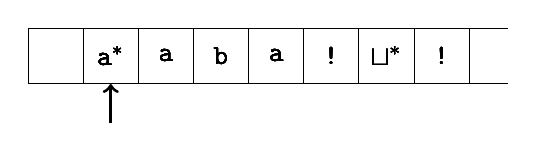
\begin{tikzpicture}

\draw (0.35, 0.35)
  node[draw, line width=0.01cm, , color=black,
       rounded corners=0cm, inner sep=0cm] {

\begin{minipage}[t][0.7cm]{0.7cm}
\mbox{}

\end{minipage}

};\draw (0.35, 0.35) node[color=black] {\texttt{\DOLLAR}};
\draw (1.0499999999999998, 0.35)
  node[draw, line width=0.01cm, , color=black,
       rounded corners=0cm, inner sep=0cm] {

\begin{minipage}[t][0.7cm]{0.7cm}
\mbox{}

\end{minipage}

};\draw (1.0499999999999998, 0.35) node[color=black] {\texttt{a$^*$}};
\draw (1.7499999999999998, 0.35)
  node[draw, line width=0.01cm, , color=black,
       rounded corners=0cm, inner sep=0cm] {

\begin{minipage}[t][0.7cm]{0.7cm}
\mbox{}

\end{minipage}

};\draw (1.7499999999999998, 0.35) node[color=black] {\texttt{a}};
\draw (2.4499999999999997, 0.35)
  node[draw, line width=0.01cm, , color=black,
       rounded corners=0cm, inner sep=0cm] {

\begin{minipage}[t][0.7cm]{0.7cm}
\mbox{}

\end{minipage}

};\draw (2.4499999999999997, 0.35) node[color=black] {\texttt{b}};
\draw (3.15, 0.35)
  node[draw, line width=0.01cm, , color=black,
       rounded corners=0cm, inner sep=0cm] {

\begin{minipage}[t][0.7cm]{0.7cm}
\mbox{}

\end{minipage}

};\draw (3.15, 0.35) node[color=black] {\texttt{a}};
\draw (3.85, 0.35)
  node[draw, line width=0.01cm, , color=black,
       rounded corners=0cm, inner sep=0cm] {

\begin{minipage}[t][0.7cm]{0.7cm}
\mbox{}

\end{minipage}

};\draw (3.85, 0.35) node[color=black] {\texttt{!}};
\draw (4.550000000000001, 0.35)
  node[draw, line width=0.01cm, , color=black,
       rounded corners=0cm, inner sep=0cm] {

\begin{minipage}[t][0.7cm]{0.7cm}
\mbox{}

\end{minipage}

};\draw (4.550000000000001, 0.35) node[color=black] {\texttt{$\sqcup^*$}};
\draw (5.25, 0.35)
  node[draw, line width=0.01cm, , color=black,
       rounded corners=0cm, inner sep=0cm] {

\begin{minipage}[t][0.7cm]{0.7cm}
\mbox{}

\end{minipage}

};\draw (5.25, 0.35) node[color=black] {\texttt{!}};
\draw (0.35, 0.35)
  node[draw, line width=0.01cm, , color=black,
       rounded corners=0cm, inner sep=0cm] {

\begin{minipage}[t][0.7cm]{0.7cm}
\mbox{}

\end{minipage}

};\draw (0.35, 0.35) node[color=black] {\texttt{\DOLLAR}};
\draw (1.0499999999999998, 0.35)
  node[draw, line width=0.01cm, , color=black,
       rounded corners=0cm, inner sep=0cm] {

\begin{minipage}[t][0.7cm]{0.7cm}
\mbox{}

\end{minipage}

};\draw (1.0499999999999998, 0.35) node[color=black] {\texttt{a$^*$}};
\draw (1.7499999999999998, 0.35)
  node[draw, line width=0.01cm, , color=black,
       rounded corners=0cm, inner sep=0cm] {

\begin{minipage}[t][0.7cm]{0.7cm}
\mbox{}

\end{minipage}

};\draw (1.7499999999999998, 0.35) node[color=black] {\texttt{a}};
\draw (2.4499999999999997, 0.35)
  node[draw, line width=0.01cm, , color=black,
       rounded corners=0cm, inner sep=0cm] {

\begin{minipage}[t][0.7cm]{0.7cm}
\mbox{}

\end{minipage}

};\draw (2.4499999999999997, 0.35) node[color=black] {\texttt{b}};
\draw (3.15, 0.35)
  node[draw, line width=0.01cm, , color=black,
       rounded corners=0cm, inner sep=0cm] {

\begin{minipage}[t][0.7cm]{0.7cm}
\mbox{}

\end{minipage}

};\draw (3.15, 0.35) node[color=black] {\texttt{a}};
\draw (3.85, 0.35)
  node[draw, line width=0.01cm, , color=black,
       rounded corners=0cm, inner sep=0cm] {

\begin{minipage}[t][0.7cm]{0.7cm}
\mbox{}

\end{minipage}

};\draw (3.85, 0.35) node[color=black] {\texttt{!}};
\draw (4.550000000000001, 0.35)
  node[draw, line width=0.01cm, , color=black,
       rounded corners=0cm, inner sep=0cm] {

\begin{minipage}[t][0.7cm]{0.7cm}
\mbox{}

\end{minipage}

};\draw (4.550000000000001, 0.35) node[color=black] {\texttt{$\sqcup^*$}};
\draw (5.25, 0.35)
  node[draw, line width=0.01cm, , color=black,
       rounded corners=0cm, inner sep=0cm] {

\begin{minipage}[t][0.7cm]{0.7cm}
\mbox{}

\end{minipage}

};\draw (5.25, 0.35) node[color=black] {\texttt{!}};
\draw (0.35, 0.35)
  node[draw, line width=0.01cm, , color=black,
       rounded corners=0cm, inner sep=0cm] {

\begin{minipage}[t][0.7cm]{0.7cm}
\mbox{}

\end{minipage}

};\draw (0.35, 0.35) node[color=black] {\texttt{\DOLLAR}};
\draw (1.0499999999999998, 0.35)
  node[draw, line width=0.01cm, , color=black,
       rounded corners=0cm, inner sep=0cm] {

\begin{minipage}[t][0.7cm]{0.7cm}
\mbox{}

\end{minipage}

};\draw (1.0499999999999998, 0.35) node[color=black] {\texttt{a$^*$}};
\draw (1.7499999999999998, 0.35)
  node[draw, line width=0.01cm, , color=black,
       rounded corners=0cm, inner sep=0cm] {

\begin{minipage}[t][0.7cm]{0.7cm}
\mbox{}

\end{minipage}

};\draw (1.7499999999999998, 0.35) node[color=black] {\texttt{a}};
\draw (2.4499999999999997, 0.35)
  node[draw, line width=0.01cm, , color=black,
       rounded corners=0cm, inner sep=0cm] {

\begin{minipage}[t][0.7cm]{0.7cm}
\mbox{}

\end{minipage}

};\draw (2.4499999999999997, 0.35) node[color=black] {\texttt{b}};
\draw (3.15, 0.35)
  node[draw, line width=0.01cm, , color=black,
       rounded corners=0cm, inner sep=0cm] {

\begin{minipage}[t][0.7cm]{0.7cm}
\mbox{}

\end{minipage}

};\draw (3.15, 0.35) node[color=black] {\texttt{a}};
\draw (3.85, 0.35)
  node[draw, line width=0.01cm, , color=black,
       rounded corners=0cm, inner sep=0cm] {

\begin{minipage}[t][0.7cm]{0.7cm}
\mbox{}

\end{minipage}

};\draw (3.85, 0.35) node[color=black] {\texttt{!}};
\draw (4.550000000000001, 0.35)
  node[draw, line width=0.01cm, , color=black,
       rounded corners=0cm, inner sep=0cm] {

\begin{minipage}[t][0.7cm]{0.7cm}
\mbox{}

\end{minipage}

};\draw (4.550000000000001, 0.35) node[color=black] {\texttt{$\sqcup^*$}};
\draw (5.25, 0.35)
  node[draw, line width=0.01cm, , color=black,
       rounded corners=0cm, inner sep=0cm] {

\begin{minipage}[t][0.7cm]{0.7cm}
\mbox{}

\end{minipage}

};\draw (5.25, 0.35) node[color=black] {\texttt{!}};
\draw (0.35, 0.35)
  node[draw, line width=0.01cm, , color=black,
       rounded corners=0cm, inner sep=0cm] {

\begin{minipage}[t][0.7cm]{0.7cm}
\mbox{}

\end{minipage}

};\draw (0.35, 0.35) node[color=black] {\texttt{\DOLLAR}};
\draw (1.0499999999999998, 0.35)
  node[draw, line width=0.01cm, , color=black,
       rounded corners=0cm, inner sep=0cm] {

\begin{minipage}[t][0.7cm]{0.7cm}
\mbox{}

\end{minipage}

};\draw (1.0499999999999998, 0.35) node[color=black] {\texttt{a$^*$}};
\draw (1.7499999999999998, 0.35)
  node[draw, line width=0.01cm, , color=black,
       rounded corners=0cm, inner sep=0cm] {

\begin{minipage}[t][0.7cm]{0.7cm}
\mbox{}

\end{minipage}

};\draw (1.7499999999999998, 0.35) node[color=black] {\texttt{a}};
\draw (2.4499999999999997, 0.35)
  node[draw, line width=0.01cm, , color=black,
       rounded corners=0cm, inner sep=0cm] {

\begin{minipage}[t][0.7cm]{0.7cm}
\mbox{}

\end{minipage}

};\draw (2.4499999999999997, 0.35) node[color=black] {\texttt{b}};
\draw (3.15, 0.35)
  node[draw, line width=0.01cm, , color=black,
       rounded corners=0cm, inner sep=0cm] {

\begin{minipage}[t][0.7cm]{0.7cm}
\mbox{}

\end{minipage}

};\draw (3.15, 0.35) node[color=black] {\texttt{a}};
\draw (3.85, 0.35)
  node[draw, line width=0.01cm, , color=black,
       rounded corners=0cm, inner sep=0cm] {

\begin{minipage}[t][0.7cm]{0.7cm}
\mbox{}

\end{minipage}

};\draw (3.85, 0.35) node[color=black] {\texttt{!}};
\draw (4.550000000000001, 0.35)
  node[draw, line width=0.01cm, , color=black,
       rounded corners=0cm, inner sep=0cm] {

\begin{minipage}[t][0.7cm]{0.7cm}
\mbox{}

\end{minipage}

};\draw (4.550000000000001, 0.35) node[color=black] {\texttt{$\sqcup^*$}};
\draw (5.25, 0.35)
  node[draw, line width=0.01cm, , color=black,
       rounded corners=0cm, inner sep=0cm] {

\begin{minipage}[t][0.7cm]{0.7cm}
\mbox{}

\end{minipage}

};\draw (5.25, 0.35) node[color=black] {\texttt{!}};
\draw (0.35, 0.35)
  node[draw, line width=0.01cm, , color=black,
       rounded corners=0cm, inner sep=0cm] {

\begin{minipage}[t][0.7cm]{0.7cm}
\mbox{}

\end{minipage}

};\draw (0.35, 0.35) node[color=black] {\texttt{\DOLLAR}};
\draw (1.0499999999999998, 0.35)
  node[draw, line width=0.01cm, , color=black,
       rounded corners=0cm, inner sep=0cm] {

\begin{minipage}[t][0.7cm]{0.7cm}
\mbox{}

\end{minipage}

};\draw (1.0499999999999998, 0.35) node[color=black] {\texttt{a$^*$}};
\draw (1.7499999999999998, 0.35)
  node[draw, line width=0.01cm, , color=black,
       rounded corners=0cm, inner sep=0cm] {

\begin{minipage}[t][0.7cm]{0.7cm}
\mbox{}

\end{minipage}

};\draw (1.7499999999999998, 0.35) node[color=black] {\texttt{a}};
\draw (2.4499999999999997, 0.35)
  node[draw, line width=0.01cm, , color=black,
       rounded corners=0cm, inner sep=0cm] {

\begin{minipage}[t][0.7cm]{0.7cm}
\mbox{}

\end{minipage}

};\draw (2.4499999999999997, 0.35) node[color=black] {\texttt{b}};
\draw (3.15, 0.35)
  node[draw, line width=0.01cm, , color=black,
       rounded corners=0cm, inner sep=0cm] {

\begin{minipage}[t][0.7cm]{0.7cm}
\mbox{}

\end{minipage}

};\draw (3.15, 0.35) node[color=black] {\texttt{a}};
\draw (3.85, 0.35)
  node[draw, line width=0.01cm, , color=black,
       rounded corners=0cm, inner sep=0cm] {

\begin{minipage}[t][0.7cm]{0.7cm}
\mbox{}

\end{minipage}

};\draw (3.85, 0.35) node[color=black] {\texttt{!}};
\draw (4.550000000000001, 0.35)
  node[draw, line width=0.01cm, , color=black,
       rounded corners=0cm, inner sep=0cm] {

\begin{minipage}[t][0.7cm]{0.7cm}
\mbox{}

\end{minipage}

};\draw (4.550000000000001, 0.35) node[color=black] {\texttt{$\sqcup^*$}};
\draw (5.25, 0.35)
  node[draw, line width=0.01cm, , color=black,
       rounded corners=0cm, inner sep=0cm] {

\begin{minipage}[t][0.7cm]{0.7cm}
\mbox{}

\end{minipage}

};\draw (5.25, 0.35) node[color=black] {\texttt{!}};
\draw (0.35, 0.35)
  node[draw, line width=0.01cm, , color=black,
       rounded corners=0cm, inner sep=0cm] {

\begin{minipage}[t][0.7cm]{0.7cm}
\mbox{}

\end{minipage}

};\draw (0.35, 0.35) node[color=black] {\texttt{\DOLLAR}};
\draw (1.0499999999999998, 0.35)
  node[draw, line width=0.01cm, , color=black,
       rounded corners=0cm, inner sep=0cm] {

\begin{minipage}[t][0.7cm]{0.7cm}
\mbox{}

\end{minipage}

};\draw (1.0499999999999998, 0.35) node[color=black] {\texttt{a$^*$}};
\draw (1.7499999999999998, 0.35)
  node[draw, line width=0.01cm, , color=black,
       rounded corners=0cm, inner sep=0cm] {

\begin{minipage}[t][0.7cm]{0.7cm}
\mbox{}

\end{minipage}

};\draw (1.7499999999999998, 0.35) node[color=black] {\texttt{a}};
\draw (2.4499999999999997, 0.35)
  node[draw, line width=0.01cm, , color=black,
       rounded corners=0cm, inner sep=0cm] {

\begin{minipage}[t][0.7cm]{0.7cm}
\mbox{}

\end{minipage}

};\draw (2.4499999999999997, 0.35) node[color=black] {\texttt{b}};
\draw (3.15, 0.35)
  node[draw, line width=0.01cm, , color=black,
       rounded corners=0cm, inner sep=0cm] {

\begin{minipage}[t][0.7cm]{0.7cm}
\mbox{}

\end{minipage}

};\draw (3.15, 0.35) node[color=black] {\texttt{a}};
\draw (3.85, 0.35)
  node[draw, line width=0.01cm, , color=black,
       rounded corners=0cm, inner sep=0cm] {

\begin{minipage}[t][0.7cm]{0.7cm}
\mbox{}

\end{minipage}

};\draw (3.85, 0.35) node[color=black] {\texttt{!}};
\draw (4.550000000000001, 0.35)
  node[draw, line width=0.01cm, , color=black,
       rounded corners=0cm, inner sep=0cm] {

\begin{minipage}[t][0.7cm]{0.7cm}
\mbox{}

\end{minipage}

};\draw (4.550000000000001, 0.35) node[color=black] {\texttt{$\sqcup^*$}};
\draw (5.25, 0.35)
  node[draw, line width=0.01cm, , color=black,
       rounded corners=0cm, inner sep=0cm] {

\begin{minipage}[t][0.7cm]{0.7cm}
\mbox{}

\end{minipage}

};\draw (5.25, 0.35) node[color=black] {\texttt{!}};
\draw (0.35, 0.35)
  node[draw, line width=0.01cm, , color=black,
       rounded corners=0cm, inner sep=0cm] {

\begin{minipage}[t][0.7cm]{0.7cm}
\mbox{}

\end{minipage}

};\draw (0.35, 0.35) node[color=black] {\texttt{\DOLLAR}};
\draw (1.0499999999999998, 0.35)
  node[draw, line width=0.01cm, , color=black,
       rounded corners=0cm, inner sep=0cm] {

\begin{minipage}[t][0.7cm]{0.7cm}
\mbox{}

\end{minipage}

};\draw (1.0499999999999998, 0.35) node[color=black] {\texttt{a$^*$}};
\draw (1.7499999999999998, 0.35)
  node[draw, line width=0.01cm, , color=black,
       rounded corners=0cm, inner sep=0cm] {

\begin{minipage}[t][0.7cm]{0.7cm}
\mbox{}

\end{minipage}

};\draw (1.7499999999999998, 0.35) node[color=black] {\texttt{a}};
\draw (2.4499999999999997, 0.35)
  node[draw, line width=0.01cm, , color=black,
       rounded corners=0cm, inner sep=0cm] {

\begin{minipage}[t][0.7cm]{0.7cm}
\mbox{}

\end{minipage}

};\draw (2.4499999999999997, 0.35) node[color=black] {\texttt{b}};
\draw (3.15, 0.35)
  node[draw, line width=0.01cm, , color=black,
       rounded corners=0cm, inner sep=0cm] {

\begin{minipage}[t][0.7cm]{0.7cm}
\mbox{}

\end{minipage}

};\draw (3.15, 0.35) node[color=black] {\texttt{a}};
\draw (3.85, 0.35)
  node[draw, line width=0.01cm, , color=black,
       rounded corners=0cm, inner sep=0cm] {

\begin{minipage}[t][0.7cm]{0.7cm}
\mbox{}

\end{minipage}

};\draw (3.85, 0.35) node[color=black] {\texttt{!}};
\draw (4.550000000000001, 0.35)
  node[draw, line width=0.01cm, , color=black,
       rounded corners=0cm, inner sep=0cm] {

\begin{minipage}[t][0.7cm]{0.7cm}
\mbox{}

\end{minipage}

};\draw (4.550000000000001, 0.35) node[color=black] {\texttt{$\sqcup^*$}};
\draw (5.25, 0.35)
  node[draw, line width=0.01cm, , color=black,
       rounded corners=0cm, inner sep=0cm] {

\begin{minipage}[t][0.7cm]{0.7cm}
\mbox{}

\end{minipage}

};\draw (5.25, 0.35) node[color=black] {\texttt{!}};
\draw (0.35, 0.35)
  node[draw, line width=0.01cm, , color=black,
       rounded corners=0cm, inner sep=0cm] {

\begin{minipage}[t][0.7cm]{0.7cm}
\mbox{}

\end{minipage}

};\draw (0.35, 0.35) node[color=black] {\texttt{\DOLLAR}};
\draw (1.0499999999999998, 0.35)
  node[draw, line width=0.01cm, , color=black,
       rounded corners=0cm, inner sep=0cm] {

\begin{minipage}[t][0.7cm]{0.7cm}
\mbox{}

\end{minipage}

};\draw (1.0499999999999998, 0.35) node[color=black] {\texttt{a$^*$}};
\draw (1.7499999999999998, 0.35)
  node[draw, line width=0.01cm, , color=black,
       rounded corners=0cm, inner sep=0cm] {

\begin{minipage}[t][0.7cm]{0.7cm}
\mbox{}

\end{minipage}

};\draw (1.7499999999999998, 0.35) node[color=black] {\texttt{a}};
\draw (2.4499999999999997, 0.35)
  node[draw, line width=0.01cm, , color=black,
       rounded corners=0cm, inner sep=0cm] {

\begin{minipage}[t][0.7cm]{0.7cm}
\mbox{}

\end{minipage}

};\draw (2.4499999999999997, 0.35) node[color=black] {\texttt{b}};
\draw (3.15, 0.35)
  node[draw, line width=0.01cm, , color=black,
       rounded corners=0cm, inner sep=0cm] {

\begin{minipage}[t][0.7cm]{0.7cm}
\mbox{}

\end{minipage}

};\draw (3.15, 0.35) node[color=black] {\texttt{a}};
\draw (3.85, 0.35)
  node[draw, line width=0.01cm, , color=black,
       rounded corners=0cm, inner sep=0cm] {

\begin{minipage}[t][0.7cm]{0.7cm}
\mbox{}

\end{minipage}

};\draw (3.85, 0.35) node[color=black] {\texttt{!}};
\draw (4.550000000000001, 0.35)
  node[draw, line width=0.01cm, , color=black,
       rounded corners=0cm, inner sep=0cm] {

\begin{minipage}[t][0.7cm]{0.7cm}
\mbox{}

\end{minipage}

};\draw (4.550000000000001, 0.35) node[color=black] {\texttt{$\sqcup^*$}};
\draw (5.25, 0.35)
  node[draw, line width=0.01cm, , color=black,
       rounded corners=0cm, inner sep=0cm] {

\begin{minipage}[t][0.7cm]{0.7cm}
\mbox{}

\end{minipage}

};\draw (5.25, 0.35) node[color=black] {\texttt{!}};\draw[line width=0.01cm,black] (5.6000000000000005,0.7) to  (6.1000000000000005,0.7);
\draw[line width=0.01cm,black] (5.6000000000000005,0.0) to  (6.1000000000000005,0.0);
\draw[line width=0.04cm,black,->] (1.05,-0.51) to  (1.05,-0.01);
\end{tikzpicture}

\end{center}




\begin{Verbatim}[frame=single]
node.remove_if_leaf()    remove the node if it's leaf.
                         Otherwise an exception it 
                         thrown.
node.remove_if_leaf(i)   remove the i-th child if the
                         child is a leaf.
node.remove_left_leaf()  remove left child if it is a 
                         leaf; if the left child is not a 
                         leaf, an exception is thrown.
node.remove_right_leaf() remove right child if it is a 
                         leaf; if the right child is not 
                         a leaf, an exception is thrown.

\end{Verbatim}

We can also move the whole tree by specifying the root.
Of course this includes the case of removing a subtree by specifying
the root of a subtree.
 % done
\newpage\input{height.tex} % done
\newpage%-*-latex-*-
\sectionthree{Copy constructor}
\begin{python0}
from solutions import *; clear()
\end{python0}

Suppose we have a tree $T$, say the pointer to the root is \verb!q! and
I want to clone $T$ to another tree where the pointer to the root is \verb!p!.
At this point, say \verb!p! has not been allocated.

{\small
\begin{Verbatim}[frame=single]
void copy_constructor(Node *& p, Node * q) 
{
    if (q == NULL)
    {
        p = NULL; 
    }
    else
    {
        p = new Node(q->key());
        // A: If node has parent pointer, then
        // make *p point to parent node
        copy_constructor(p->left_, q->left_);
        copy_constructor(p->right_, q->right_);
    }
}
\end{Verbatim}
}
At A, we have a problem: How do we set \verb!*p! to point to its parent?
Of course if our nodes do not have parent pointers, then we can forget about A.

\textsc{Method 1.}
One way is to pass the address of the parent into the function:
{\small
\begin{Verbatim}[frame=single]
void copy_constructor(Node *& parent, Node *& p, Node * q) 
{
    ...
    else
    {
        p = new Node(q->key());
        p->parent = parent;
        copy_constructor(p, p->left_, q->left_);
        copy_constructor(p, p->right_, q->right_);
    }
}
\end{Verbatim}
}

\textsc{Method 2.}
The other way is to ensure that the function is clone the child node of \verb!q!
to a child node of \verb!p!, i.e.,
\verb!p! is the parent pointer of the node being cloned.
In this way, the parent is still in scope.
{\small
\begin{Verbatim}[frame=single]
void copy_constructor(Node *& p, Node * q)
{
    if (q == NULL)
    {
        p = NULL;
    }
    else
    {
        p = new Node;
        p->key_ = q->key_;
        copy_constructor_(p, q);
    }
}
void copy_constructor_(Node *& p, Node * q) 
{
    if (q->left_ != NULL)
    {
        p->left_ = new Node(q->left_->key());
        p->left_->parent = p;
        copy_constructor(p->left_, q->left_);
    }
    if (q->right_ != NULL)
    {
        p->right_ = new Node(q->right_->key());
        p->right_->parent = p;
        copy_constructor(p->right_, q->right_);
    }
}
\end{Verbatim}
}

\textsc{Method 3.}
Here's a third way to make a copy of the a binary tree.
In this case the address of the root is returned.
{\small
\begin{Verbatim}[frame=single]
Node * copy_constructor(Node * q)
{
    if (q == NULL)
    {
        return NULL;
    }
    else
    {
        Node * pleft = copy_constructor(q->left_);
        Node * pright = copy_constructor(q->right_);
        Node * p = new Node(q->key_, NULL, pleft, pright);
        if (pleft != NULL) pleft->parent_ = p;
        if (pright != NULL) pright->parent_ = p;
        return p;
    }
}
\end{Verbatim}
}
 % done
\newpage%-*-latex-*-
\sectionthree{Destructor/deallocation}
\begin{python0}
from solutions import *; clear()
\end{python0}

Suppose you have a tree $T$ in the heap.
Say a pointer \verb!p! points to the root of the tree (with
value $\alpha$ in the diagram):


\begin{center}
\begin{tikzpicture}[>=triangle 60,shorten >=0.5pt,node distance=2cm,auto,initial text=, double distance=2pt]
\node[state,initial] (A) at (  0,  0) {};

\path[->]
(A) edge [loop above] node {$a,b$} ()

;
\end{tikzpicture}
\end{center}
    


The memory used by the node (with value $\alpha$) and the
subtrees ($T_1$ and $T_2$) must all be returned to the heap.
Suppose the function is called \verb!deallocate! and the
parameter the a pointer to the root.
{\small
\begin{Verbatim}
    deallocate(p);
\end{Verbatim}
}
Of course this would result in
{\small
\begin{Verbatim}
    delete p;
    deallocate(q);
    deallocate(r);
\end{Verbatim}
}
where \verb!q! and \verb!r! are pointers to the left and right
subtrees of node with value $\alpha$.
Therefore the code would look like:
{\small
\begin{Verbatim}[frame=single]
void deallocate(Node * p)
{
    if (p != NULL)
    {
        deallocate(p->left_);
        deallocate(p->right_);
        delete p;
    }
}
\end{Verbatim}
}
Of course you \textit{cannot} do this:
{\small
\begin{Verbatim}[frame=single]
void deallocate(Node * p)
{
    if (p != NULL)
    {
        delete p;
        deallocate(p->left_);
        deallocate(p->right_);
    }
}
\end{Verbatim}
}
Do you see why?


The above is for the case where the tree is a binary tree.
It's clear what you need to do for a general tree.

Notice that the above uses the postorder traveral on the tree, i.e.,
we perform a postorder traveral of the tree and
perform deallocate the memory
used by each node.

Note that if you have a tree class (for instance a binary tree class):
{\small
\begin{Verbatim}[frame=single]
class Tree
{
private:
    Node * proot_;
};
\end{Verbatim}
}
the destructor can then be
{\small
\begin{Verbatim}[frame=single]
class Tree
{
public:
    ...
    ~Tree()
    {
        deallocate(proot_);
    }
...
};
\end{Verbatim}
}
You should probably also have a method to clear the tree:
{\small
\begin{Verbatim}[frame=single]
class Tree
{
public:
    ...
    void clear()
    {
        deallocate(proot_);
        proot_ = NULL;
    }
...
};
\end{Verbatim}
}
This is sort of like the destructor except that the tree object does not go out of
scope and you are in control of calling this method.

 % done
\newpage%-*-latex-*-
\sectionthree{Application: prefix tree}
\begin{python0}
from solutions import *; clear()
\end{python0}

A \defone{prefix tree} or a \defone{trie} is a tree for storing data with
lots of common prefixes.
What instance the word \texttt{cat} and \texttt{cab}
share a common prefix of \texttt{ca}.

As an example, say I want to store a list of words
in lowercase.
I use this
\begin{console}
class Node
{
public:
    char flag;
    Node * v[26];
};
\end{console}
Note that each node has 26 pointers, i.e., 26 edges going
to 26 children, each pointer corresponding to one fo the lower case letter.
Say I want to store the words \texttt{cab}, \texttt{cat}, \texttt{catch}.
Here's the picture:
\begin{console}[frame=single,fontsize=\footnotesize]
[student@localhost forward_list] g++ main.cpp; ./a.out
1.
true
size: 0
[3, 2, 1, 0]
[]
2.
[1, 2, 3, 4]
[2, 3, 4]
3.
[1, 2, 3, 4]
42
[42, 2, 3, 4]
4.
[1, 2, 3, 4]
[1, 2, 4]
5.
[1, 2, 3, 4]
[1, 2]
6.
[1, 2, 3, 4]
[1, 2, 77777, 88888, 99999, 3, 4]
7.
[1, 2, 3, 4]
[1, 2, -1, -1, -1, -1, -1, 3, 4]
8.
[1, 2, 3, 4]
[1, 2, 88, 99, 3, 4]
\end{console}


What this means is that from the root node, say I call it
\verb!r!, there's an edge corresponding
to a pointer \verb!r.v[2]! (2 corresponding to \texttt{c})
that points to a node, say I call it \texttt{s}.
\texttt{s.v[0]} (0 corresponding to \texttt{a})
pointing to a node, say I call it \texttt{t}.
Etc.
If the node's flag is \texttt{*}, then it means that
I've reached a word when I start from the root.

When I draw this this edge between the lowest two nodes:

\begin{console}[frame=single,fontsize=\footnotesize]
[student@localhost list] g++ main.cpp; ./a.out
1.
true
size: 0
[1, 0, 111, 222]
2.
[1, 2, 3, 4]
[2, 3]
3.
[1, 2, 3, 4]
[111, 2, 3, 999]
4.
[1, 2, 3, 4]
[1, 3, 4]
[1, 3, 4]
5.
[1, 2, 3, 4]
[1, 4]
6.
[1, 2, 3, 4]
[1, 99999, 88888, 77777, 2, 3, 4]
7.
[1, 2, 3, 4]
[1, -1, -1, -1, -1, -1, 2, 3, 4]
8.
[1, 2, 3, 4]
[1, 88, 99, 2, 3, 4]
9.
[1, 2, 3, 4]
4 3 2 1
\end{console}



I mean this:

\begin{center}
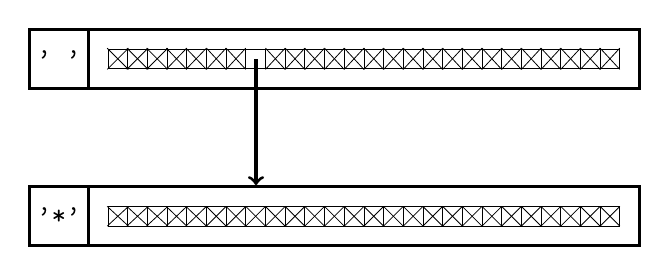
\begin{tikzpicture}

\draw (0.125, 0.125)
  node[draw, line width=0.01cm, , color=black,
       rounded corners=0cm, inner sep=0cm] {

\begin{minipage}[t][0.25cm]{0.25cm}
\mbox{}

\end{minipage}

};
\draw (0.375, 0.125)
  node[draw, line width=0.01cm, , color=black,
       rounded corners=0cm, inner sep=0cm] {

\begin{minipage}[t][0.25cm]{0.25cm}
\mbox{}

\end{minipage}

};
\draw (0.625, 0.125)
  node[draw, line width=0.01cm, , color=black,
       rounded corners=0cm, inner sep=0cm] {

\begin{minipage}[t][0.25cm]{0.25cm}
\mbox{}

\end{minipage}

};
\draw (0.875, 0.125)
  node[draw, line width=0.01cm, , color=black,
       rounded corners=0cm, inner sep=0cm] {

\begin{minipage}[t][0.25cm]{0.25cm}
\mbox{}

\end{minipage}

};
\draw (1.125, 0.125)
  node[draw, line width=0.01cm, , color=black,
       rounded corners=0cm, inner sep=0cm] {

\begin{minipage}[t][0.25cm]{0.25cm}
\mbox{}

\end{minipage}

};
\draw (1.375, 0.125)
  node[draw, line width=0.01cm, , color=black,
       rounded corners=0cm, inner sep=0cm] {

\begin{minipage}[t][0.25cm]{0.25cm}
\mbox{}

\end{minipage}

};
\draw (1.625, 0.125)
  node[draw, line width=0.01cm, , color=black,
       rounded corners=0cm, inner sep=0cm] {

\begin{minipage}[t][0.25cm]{0.25cm}
\mbox{}

\end{minipage}

};
\draw (1.875, 0.125)
  node[draw, line width=0.01cm, , color=black,
       rounded corners=0cm, inner sep=0cm] {

\begin{minipage}[t][0.25cm]{0.25cm}
\mbox{}

\end{minipage}

};
\draw (2.125, 0.125)
  node[draw, line width=0.01cm, , color=black,
       rounded corners=0cm, inner sep=0cm] {

\begin{minipage}[t][0.25cm]{0.25cm}
\mbox{}

\end{minipage}

};
\draw (2.375, 0.125)
  node[draw, line width=0.01cm, , color=black,
       rounded corners=0cm, inner sep=0cm] {

\begin{minipage}[t][0.25cm]{0.25cm}
\mbox{}

\end{minipage}

};
\draw (2.625, 0.125)
  node[draw, line width=0.01cm, , color=black,
       rounded corners=0cm, inner sep=0cm] {

\begin{minipage}[t][0.25cm]{0.25cm}
\mbox{}

\end{minipage}

};
\draw (2.875, 0.125)
  node[draw, line width=0.01cm, , color=black,
       rounded corners=0cm, inner sep=0cm] {

\begin{minipage}[t][0.25cm]{0.25cm}
\mbox{}

\end{minipage}

};
\draw (3.125, 0.125)
  node[draw, line width=0.01cm, , color=black,
       rounded corners=0cm, inner sep=0cm] {

\begin{minipage}[t][0.25cm]{0.25cm}
\mbox{}

\end{minipage}

};
\draw (3.375, 0.125)
  node[draw, line width=0.01cm, , color=black,
       rounded corners=0cm, inner sep=0cm] {

\begin{minipage}[t][0.25cm]{0.25cm}
\mbox{}

\end{minipage}

};
\draw (3.625, 0.125)
  node[draw, line width=0.01cm, , color=black,
       rounded corners=0cm, inner sep=0cm] {

\begin{minipage}[t][0.25cm]{0.25cm}
\mbox{}

\end{minipage}

};
\draw (3.875, 0.125)
  node[draw, line width=0.01cm, , color=black,
       rounded corners=0cm, inner sep=0cm] {

\begin{minipage}[t][0.25cm]{0.25cm}
\mbox{}

\end{minipage}

};
\draw (4.125, 0.125)
  node[draw, line width=0.01cm, , color=black,
       rounded corners=0cm, inner sep=0cm] {

\begin{minipage}[t][0.25cm]{0.25cm}
\mbox{}

\end{minipage}

};
\draw (4.375, 0.125)
  node[draw, line width=0.01cm, , color=black,
       rounded corners=0cm, inner sep=0cm] {

\begin{minipage}[t][0.25cm]{0.25cm}
\mbox{}

\end{minipage}

};
\draw (4.625, 0.125)
  node[draw, line width=0.01cm, , color=black,
       rounded corners=0cm, inner sep=0cm] {

\begin{minipage}[t][0.25cm]{0.25cm}
\mbox{}

\end{minipage}

};
\draw (4.875, 0.125)
  node[draw, line width=0.01cm, , color=black,
       rounded corners=0cm, inner sep=0cm] {

\begin{minipage}[t][0.25cm]{0.25cm}
\mbox{}

\end{minipage}

};
\draw (5.125, 0.125)
  node[draw, line width=0.01cm, , color=black,
       rounded corners=0cm, inner sep=0cm] {

\begin{minipage}[t][0.25cm]{0.25cm}
\mbox{}

\end{minipage}

};
\draw (5.375, 0.125)
  node[draw, line width=0.01cm, , color=black,
       rounded corners=0cm, inner sep=0cm] {

\begin{minipage}[t][0.25cm]{0.25cm}
\mbox{}

\end{minipage}

};
\draw (5.625, 0.125)
  node[draw, line width=0.01cm, , color=black,
       rounded corners=0cm, inner sep=0cm] {

\begin{minipage}[t][0.25cm]{0.25cm}
\mbox{}

\end{minipage}

};
\draw (5.875, 0.125)
  node[draw, line width=0.01cm, , color=black,
       rounded corners=0cm, inner sep=0cm] {

\begin{minipage}[t][0.25cm]{0.25cm}
\mbox{}

\end{minipage}

};
\draw (6.125, 0.125)
  node[draw, line width=0.01cm, , color=black,
       rounded corners=0cm, inner sep=0cm] {

\begin{minipage}[t][0.25cm]{0.25cm}
\mbox{}

\end{minipage}

};
\draw (6.375, 0.125)
  node[draw, line width=0.01cm, , color=black,
       rounded corners=0cm, inner sep=0cm] {

\begin{minipage}[t][0.25cm]{0.25cm}
\mbox{}

\end{minipage}

};
\draw (3.25, 0.125)
  node[draw, line width=0.04cm, , color=black,
       rounded corners=0cm, inner sep=0cm] {

\begin{minipage}[t][0.75cm]{7.0cm}
\mbox{}

\end{minipage}

};\draw[line width=0.01cm,black] (-0.01,0.26) to  (0.26,-0.01);
\draw[line width=0.01cm,black] (0.26,0.26) to  (-0.01,-0.01);
\draw[line width=0.01cm,black] (0.24,0.26) to  (0.51,-0.01);
\draw[line width=0.01cm,black] (0.51,0.26) to  (0.24,-0.01);
\draw[line width=0.01cm,black] (0.49,0.26) to  (0.76,-0.01);
\draw[line width=0.01cm,black] (0.76,0.26) to  (0.49,-0.01);
\draw[line width=0.01cm,black] (0.74,0.26) to  (1.0,-0.01);
\draw[line width=0.01cm,black] (1.0,0.26) to  (0.74,-0.01);
\draw[line width=0.01cm,black] (0.99,0.26) to  (1.25,-0.01);
\draw[line width=0.01cm,black] (1.25,0.26) to  (0.99,-0.01);
\draw[line width=0.01cm,black] (1.25,0.26) to  (1.5,-0.01);
\draw[line width=0.01cm,black] (1.5,0.26) to  (1.25,-0.01);
\draw[line width=0.01cm,black] (1.5,0.26) to  (1.75,-0.01);
\draw[line width=0.01cm,black] (1.75,0.26) to  (1.5,-0.01);
\draw[line width=0.01cm,black] (2.0,0.26) to  (2.25,-0.01);
\draw[line width=0.01cm,black] (2.25,0.26) to  (2.0,-0.01);
\draw[line width=0.01cm,black] (2.25,0.26) to  (2.5,-0.01);
\draw[line width=0.01cm,black] (2.5,0.26) to  (2.25,-0.01);
\draw[line width=0.01cm,black] (2.5,0.26) to  (2.75,-0.01);
\draw[line width=0.01cm,black] (2.75,0.26) to  (2.5,-0.01);
\draw[line width=0.01cm,black] (2.75,0.26) to  (3.0,-0.01);
\draw[line width=0.01cm,black] (3.0,0.26) to  (2.75,-0.01);
\draw[line width=0.01cm,black] (3.0,0.26) to  (3.25,-0.01);
\draw[line width=0.01cm,black] (3.25,0.26) to  (3.0,-0.01);
\draw[line width=0.01cm,black] (3.25,0.26) to  (3.5,-0.01);
\draw[line width=0.01cm,black] (3.5,0.26) to  (3.25,-0.01);
\draw[line width=0.01cm,black] (3.5,0.26) to  (3.75,-0.01);
\draw[line width=0.01cm,black] (3.75,0.26) to  (3.5,-0.01);
\draw[line width=0.01cm,black] (3.75,0.26) to  (4.0,-0.01);
\draw[line width=0.01cm,black] (4.0,0.26) to  (3.75,-0.01);
\draw[line width=0.01cm,black] (4.0,0.26) to  (4.25,-0.01);
\draw[line width=0.01cm,black] (4.25,0.26) to  (4.0,-0.01);
\draw[line width=0.01cm,black] (4.25,0.26) to  (4.5,-0.01);
\draw[line width=0.01cm,black] (4.5,0.26) to  (4.25,-0.01);
\draw[line width=0.01cm,black] (4.5,0.26) to  (4.75,-0.01);
\draw[line width=0.01cm,black] (4.75,0.26) to  (4.5,-0.01);
\draw[line width=0.01cm,black] (4.75,0.26) to  (5.0,-0.01);
\draw[line width=0.01cm,black] (5.0,0.26) to  (4.75,-0.01);
\draw[line width=0.01cm,black] (5.0,0.26) to  (5.25,-0.01);
\draw[line width=0.01cm,black] (5.25,0.26) to  (5.0,-0.01);
\draw[line width=0.01cm,black] (5.25,0.26) to  (5.5,-0.01);
\draw[line width=0.01cm,black] (5.5,0.26) to  (5.25,-0.01);
\draw[line width=0.01cm,black] (5.5,0.26) to  (5.75,-0.01);
\draw[line width=0.01cm,black] (5.75,0.26) to  (5.5,-0.01);
\draw[line width=0.01cm,black] (5.75,0.26) to  (6.0,-0.01);
\draw[line width=0.01cm,black] (6.0,0.26) to  (5.75,-0.01);
\draw[line width=0.01cm,black] (6.0,0.26) to  (6.25,-0.01);
\draw[line width=0.01cm,black] (6.25,0.26) to  (6.0,-0.01);
\draw[line width=0.01cm,black] (6.25,0.26) to  (6.5,-0.01);
\draw[line width=0.01cm,black] (6.5,0.26) to  (6.25,-0.01);

\draw (-0.625, 0.125)
  node[draw, line width=0.04cm, , color=black,
       rounded corners=0cm, inner sep=0cm] {

\begin{minipage}[t][0.75cm]{0.75cm}
\mbox{}

\end{minipage}

};\draw (-0.625, 0.125) node[color=black] {\texttt{' '}};
\draw (0.125, -1.875)
  node[draw, line width=0.01cm, , color=black,
       rounded corners=0cm, inner sep=0cm] {

\begin{minipage}[t][0.25cm]{0.25cm}
\mbox{}

\end{minipage}

};
\draw (0.375, -1.875)
  node[draw, line width=0.01cm, , color=black,
       rounded corners=0cm, inner sep=0cm] {

\begin{minipage}[t][0.25cm]{0.25cm}
\mbox{}

\end{minipage}

};
\draw (0.625, -1.875)
  node[draw, line width=0.01cm, , color=black,
       rounded corners=0cm, inner sep=0cm] {

\begin{minipage}[t][0.25cm]{0.25cm}
\mbox{}

\end{minipage}

};
\draw (0.875, -1.875)
  node[draw, line width=0.01cm, , color=black,
       rounded corners=0cm, inner sep=0cm] {

\begin{minipage}[t][0.25cm]{0.25cm}
\mbox{}

\end{minipage}

};
\draw (1.125, -1.875)
  node[draw, line width=0.01cm, , color=black,
       rounded corners=0cm, inner sep=0cm] {

\begin{minipage}[t][0.25cm]{0.25cm}
\mbox{}

\end{minipage}

};
\draw (1.375, -1.875)
  node[draw, line width=0.01cm, , color=black,
       rounded corners=0cm, inner sep=0cm] {

\begin{minipage}[t][0.25cm]{0.25cm}
\mbox{}

\end{minipage}

};
\draw (1.625, -1.875)
  node[draw, line width=0.01cm, , color=black,
       rounded corners=0cm, inner sep=0cm] {

\begin{minipage}[t][0.25cm]{0.25cm}
\mbox{}

\end{minipage}

};
\draw (1.875, -1.875)
  node[draw, line width=0.01cm, , color=black,
       rounded corners=0cm, inner sep=0cm] {

\begin{minipage}[t][0.25cm]{0.25cm}
\mbox{}

\end{minipage}

};
\draw (2.125, -1.875)
  node[draw, line width=0.01cm, , color=black,
       rounded corners=0cm, inner sep=0cm] {

\begin{minipage}[t][0.25cm]{0.25cm}
\mbox{}

\end{minipage}

};
\draw (2.375, -1.875)
  node[draw, line width=0.01cm, , color=black,
       rounded corners=0cm, inner sep=0cm] {

\begin{minipage}[t][0.25cm]{0.25cm}
\mbox{}

\end{minipage}

};
\draw (2.625, -1.875)
  node[draw, line width=0.01cm, , color=black,
       rounded corners=0cm, inner sep=0cm] {

\begin{minipage}[t][0.25cm]{0.25cm}
\mbox{}

\end{minipage}

};
\draw (2.875, -1.875)
  node[draw, line width=0.01cm, , color=black,
       rounded corners=0cm, inner sep=0cm] {

\begin{minipage}[t][0.25cm]{0.25cm}
\mbox{}

\end{minipage}

};
\draw (3.125, -1.875)
  node[draw, line width=0.01cm, , color=black,
       rounded corners=0cm, inner sep=0cm] {

\begin{minipage}[t][0.25cm]{0.25cm}
\mbox{}

\end{minipage}

};
\draw (3.375, -1.875)
  node[draw, line width=0.01cm, , color=black,
       rounded corners=0cm, inner sep=0cm] {

\begin{minipage}[t][0.25cm]{0.25cm}
\mbox{}

\end{minipage}

};
\draw (3.625, -1.875)
  node[draw, line width=0.01cm, , color=black,
       rounded corners=0cm, inner sep=0cm] {

\begin{minipage}[t][0.25cm]{0.25cm}
\mbox{}

\end{minipage}

};
\draw (3.875, -1.875)
  node[draw, line width=0.01cm, , color=black,
       rounded corners=0cm, inner sep=0cm] {

\begin{minipage}[t][0.25cm]{0.25cm}
\mbox{}

\end{minipage}

};
\draw (4.125, -1.875)
  node[draw, line width=0.01cm, , color=black,
       rounded corners=0cm, inner sep=0cm] {

\begin{minipage}[t][0.25cm]{0.25cm}
\mbox{}

\end{minipage}

};
\draw (4.375, -1.875)
  node[draw, line width=0.01cm, , color=black,
       rounded corners=0cm, inner sep=0cm] {

\begin{minipage}[t][0.25cm]{0.25cm}
\mbox{}

\end{minipage}

};
\draw (4.625, -1.875)
  node[draw, line width=0.01cm, , color=black,
       rounded corners=0cm, inner sep=0cm] {

\begin{minipage}[t][0.25cm]{0.25cm}
\mbox{}

\end{minipage}

};
\draw (4.875, -1.875)
  node[draw, line width=0.01cm, , color=black,
       rounded corners=0cm, inner sep=0cm] {

\begin{minipage}[t][0.25cm]{0.25cm}
\mbox{}

\end{minipage}

};
\draw (5.125, -1.875)
  node[draw, line width=0.01cm, , color=black,
       rounded corners=0cm, inner sep=0cm] {

\begin{minipage}[t][0.25cm]{0.25cm}
\mbox{}

\end{minipage}

};
\draw (5.375, -1.875)
  node[draw, line width=0.01cm, , color=black,
       rounded corners=0cm, inner sep=0cm] {

\begin{minipage}[t][0.25cm]{0.25cm}
\mbox{}

\end{minipage}

};
\draw (5.625, -1.875)
  node[draw, line width=0.01cm, , color=black,
       rounded corners=0cm, inner sep=0cm] {

\begin{minipage}[t][0.25cm]{0.25cm}
\mbox{}

\end{minipage}

};
\draw (5.875, -1.875)
  node[draw, line width=0.01cm, , color=black,
       rounded corners=0cm, inner sep=0cm] {

\begin{minipage}[t][0.25cm]{0.25cm}
\mbox{}

\end{minipage}

};
\draw (6.125, -1.875)
  node[draw, line width=0.01cm, , color=black,
       rounded corners=0cm, inner sep=0cm] {

\begin{minipage}[t][0.25cm]{0.25cm}
\mbox{}

\end{minipage}

};
\draw (6.375, -1.875)
  node[draw, line width=0.01cm, , color=black,
       rounded corners=0cm, inner sep=0cm] {

\begin{minipage}[t][0.25cm]{0.25cm}
\mbox{}

\end{minipage}

};
\draw (3.25, -1.875)
  node[draw, line width=0.04cm, , color=black,
       rounded corners=0cm, inner sep=0cm] {

\begin{minipage}[t][0.75cm]{7.0cm}
\mbox{}

\end{minipage}

};\draw[line width=0.01cm,black] (-0.01,-1.75) to  (0.26,-2.0);
\draw[line width=0.01cm,black] (0.26,-1.75) to  (-0.01,-2.0);
\draw[line width=0.01cm,black] (0.24,-1.75) to  (0.51,-2.0);
\draw[line width=0.01cm,black] (0.51,-1.75) to  (0.24,-2.0);
\draw[line width=0.01cm,black] (0.49,-1.75) to  (0.76,-2.0);
\draw[line width=0.01cm,black] (0.76,-1.75) to  (0.49,-2.0);
\draw[line width=0.01cm,black] (0.74,-1.75) to  (1.0,-2.0);
\draw[line width=0.01cm,black] (1.0,-1.75) to  (0.74,-2.0);
\draw[line width=0.01cm,black] (0.99,-1.75) to  (1.25,-2.0);
\draw[line width=0.01cm,black] (1.25,-1.75) to  (0.99,-2.0);
\draw[line width=0.01cm,black] (1.25,-1.75) to  (1.5,-2.0);
\draw[line width=0.01cm,black] (1.5,-1.75) to  (1.25,-2.0);
\draw[line width=0.01cm,black] (1.5,-1.75) to  (1.75,-2.0);
\draw[line width=0.01cm,black] (1.75,-1.75) to  (1.5,-2.0);
\draw[line width=0.01cm,black] (1.75,-1.75) to  (2.0,-2.0);
\draw[line width=0.01cm,black] (2.0,-1.75) to  (1.75,-2.0);
\draw[line width=0.01cm,black] (2.0,-1.75) to  (2.25,-2.0);
\draw[line width=0.01cm,black] (2.25,-1.75) to  (2.0,-2.0);
\draw[line width=0.01cm,black] (2.25,-1.75) to  (2.5,-2.0);
\draw[line width=0.01cm,black] (2.5,-1.75) to  (2.25,-2.0);
\draw[line width=0.01cm,black] (2.5,-1.75) to  (2.75,-2.0);
\draw[line width=0.01cm,black] (2.75,-1.75) to  (2.5,-2.0);
\draw[line width=0.01cm,black] (2.75,-1.75) to  (3.0,-2.0);
\draw[line width=0.01cm,black] (3.0,-1.75) to  (2.75,-2.0);
\draw[line width=0.01cm,black] (3.0,-1.75) to  (3.25,-2.0);
\draw[line width=0.01cm,black] (3.25,-1.75) to  (3.0,-2.0);
\draw[line width=0.01cm,black] (3.25,-1.75) to  (3.5,-2.0);
\draw[line width=0.01cm,black] (3.5,-1.75) to  (3.25,-2.0);
\draw[line width=0.01cm,black] (3.5,-1.75) to  (3.75,-2.0);
\draw[line width=0.01cm,black] (3.75,-1.75) to  (3.5,-2.0);
\draw[line width=0.01cm,black] (3.75,-1.75) to  (4.0,-2.0);
\draw[line width=0.01cm,black] (4.0,-1.75) to  (3.75,-2.0);
\draw[line width=0.01cm,black] (4.0,-1.75) to  (4.25,-2.0);
\draw[line width=0.01cm,black] (4.25,-1.75) to  (4.0,-2.0);
\draw[line width=0.01cm,black] (4.25,-1.75) to  (4.5,-2.0);
\draw[line width=0.01cm,black] (4.5,-1.75) to  (4.25,-2.0);
\draw[line width=0.01cm,black] (4.5,-1.75) to  (4.75,-2.0);
\draw[line width=0.01cm,black] (4.75,-1.75) to  (4.5,-2.0);
\draw[line width=0.01cm,black] (4.75,-1.75) to  (5.0,-2.0);
\draw[line width=0.01cm,black] (5.0,-1.75) to  (4.75,-2.0);
\draw[line width=0.01cm,black] (5.0,-1.75) to  (5.25,-2.0);
\draw[line width=0.01cm,black] (5.25,-1.75) to  (5.0,-2.0);
\draw[line width=0.01cm,black] (5.25,-1.75) to  (5.5,-2.0);
\draw[line width=0.01cm,black] (5.5,-1.75) to  (5.25,-2.0);
\draw[line width=0.01cm,black] (5.5,-1.75) to  (5.75,-2.0);
\draw[line width=0.01cm,black] (5.75,-1.75) to  (5.5,-2.0);
\draw[line width=0.01cm,black] (5.75,-1.75) to  (6.0,-2.0);
\draw[line width=0.01cm,black] (6.0,-1.75) to  (5.75,-2.0);
\draw[line width=0.01cm,black] (6.0,-1.75) to  (6.25,-2.0);
\draw[line width=0.01cm,black] (6.25,-1.75) to  (6.0,-2.0);
\draw[line width=0.01cm,black] (6.25,-1.75) to  (6.5,-2.0);
\draw[line width=0.01cm,black] (6.5,-1.75) to  (6.25,-2.0);

\draw (-0.625, -1.875)
  node[draw, line width=0.04cm, , color=black,
       rounded corners=0cm, inner sep=0cm] {

\begin{minipage}[t][0.75cm]{0.75cm}
\mbox{}

\end{minipage}

};\draw (-0.625, -1.875) node[color=black] {\texttt{'*'}};\draw[line width=0.04cm,black,->] (1.88,0.12) to  (1.88,-1.48);
\end{tikzpicture}

\end{center}



i.e., each node has a character and a vector of 26 pointers.
The node at the top has a character value of \verb!' '! and for the vector
of pointers, 25 of them at \texttt{NULL} while the
pointer at index 7 (which corresponds to character \texttt{h})
points to the next node which contains a character value of \texttt{*}
a vector of 26 pointers, all of which are \texttt{NULL}.

Get it? Neat right?

Note that the prefix above is a 26-ary tree since
each edge corresponds to one of the lowecase letter.
(If you want lower and upper case, then it's a 52-ary tree.)

\begin{ex}
Build a prefix tree for \texttt{cab}, \texttt{cat} and
\texttt{catch} using the class above.
Do it with this function:
\begin{Verbatim}[frame=single]
void insert(Node ** p, const std::string & word);
\end{Verbatim}
Write a function that accepts a string (use
\texttt{std::string}) and checks if the word
is stored in the prefix tree.
In other words when you call the function with \texttt{cat}
it returns \texttt{true};
if you call the function with \texttt{cas} is returns \texttt{false}.
Here's an appropriate prototype:
\begin{Verbatim}[frame=single]
bool is_found(const Node * const, const std::string &);
\end{Verbatim}
\qed
\end{ex}

\begin{ex}
In case you added a wrong word, you want to be able to remove a
\lq\lq word''. So do this:
\begin{Verbatim}[frame=single]
void delete(Node ** p; const std::string & word);
\end{Verbatim}
Fail silently, i.e., if you attempt to delete a word not in the
prefix tree, don't throw an exception.
Also, reclaim memory as much as you can. For instance in the above
prefix tree:
\begin{console}[frame=single,fontsize=\footnotesize]
[student@localhost stack] g++ main.cpp; ./a.out
42 42
2 2
0 0
5 5
1 1
0 0
\end{console}


if you delete the word \texttt{catch}, the
memory model of the prefix tree should be

\begin{center}

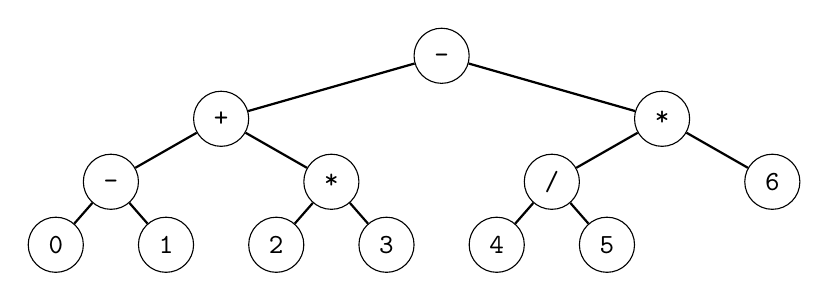
\begin{tikzpicture}
\node at (4.8999999999999995,-0.8) [circle,draw,minimum size=7mm] (A) {\texttt{-}};
\node at (2.0999999999999996,-1.6) [circle,draw,minimum size=7mm] (B) {\texttt{+}};
\node at (7.699999999999999,-1.6) [circle,draw,minimum size=7mm] (C) {\texttt{*}};
\node at (0.7,-2.4000000000000004) [circle,draw,minimum size=7mm] (D) {\texttt{-}};
\node at (3.5,-2.4000000000000004) [circle,draw,minimum size=7mm] (E) {\texttt{*}};
\node at (6.3,-2.4000000000000004) [circle,draw,minimum size=7mm] (F) {\texttt{/}};
\node at (9.1,-2.4000000000000004) [circle,draw,minimum size=7mm] (G) {\texttt{6}};
\node at (0.0,-3.2) [circle,draw,minimum size=7mm] (H) {\texttt{0}};
\node at (1.4,-3.2) [circle,draw,minimum size=7mm] (I) {\texttt{1}};
\node at (2.8,-3.2) [circle,draw,minimum size=7mm] (J) {\texttt{2}};
\node at (4.199999999999999,-3.2) [circle,draw,minimum size=7mm] (K) {\texttt{3}};
\node at (5.6,-3.2) [circle,draw,minimum size=7mm] (L) {\texttt{4}};
\node at (7.0,-3.2) [circle,draw,minimum size=7mm] (M) {\texttt{5}};
\draw [-,thick] (A) -- (B);
\draw [-,thick] (A) -- (C);
\draw [-,thick] (B) -- (D);
\draw [-,thick] (B) -- (E);
\draw [-,thick] (C) -- (F);
\draw [-,thick] (C) -- (G);
\draw [-,thick] (D) -- (H);
\draw [-,thick] (D) -- (I);
\draw [-,thick] (E) -- (J);
\draw [-,thick] (E) -- (K);
\draw [-,thick] (F) -- (L);
\draw [-,thick] (F) -- (M);

;
\end{tikzpicture}
    
\end{center}


In particular, the node that the edge labeled \texttt{t} reaches
has a vector of 26 \verb!NULL! pointers.
It's not enough just to make the character in the node that the
ledge labeled \texttt{h} leads to with a space.
\qed
\end{ex}

Because words in English (and many other languages too)
contains lots of common prefixes,
this is a very efficient way of storing words
and therefore can be used to create dictionaries.

Not only that, this is also how
word autocompletion works inside programs.
If you type part of a word into a software, the program
can sometimes give you a list of options to complete the word
once the number of options is small enough.
How does it know?
Well, as you type, the program walks down the above
tree.
From where you stop typing,
it can perform a traversal of the subtree where
the root corresponds to where you stopped.
In the traversal, when it sees a \texttt{*}
it knows that it's a word (from the root of the subtree to that node). 
Therefore the program can collect a list of
words with the same prefix as what you have typed.
The program then shows you the options.
Neat right?

\begin{ex}
Continuing the above
exercise,
write a function that
gives you a list of word completion.
if you call the function with \texttt{ca}
it returns an array (use \texttt{std::vector})
containing \texttt{cat} and \texttt{catch}.
\qed
\end{ex}

\begin{ex}
Download a dictionary file from the web.
Convert all uppercase to lowercase.
How many bytes are there in the file.
Next, build a prefix tree and then compute the
amount of memory used.
How much memory do you save?
\qed
\end{ex}

Instead of having a vector for pointers where there's one pointer
\textit{every} character \texttt{a..z},
you can have a vector of (character, pointer)  only for characters that
are actually used.
In that case the root node in the above prefix tree has only
one pointer and not 26.
However this will slow you down when you look for the word.
You can use a sorted \texttt{std::vector} to speed up the search.
This will of course save you on memory.
This is again the story of the life of algorithms:
it's always about the balance between speed and memory.
 % done
\newpage%-*-latex-*-
\sectionthree{Binary Search Tree}
\begin{python0}
from solutions import *; clear()
\end{python0}

A \defone{binary search tree} (BST)
is a binary tree where every node contains data in such a way that
\begin{itemize}
\li $T$ is an empty tree, or
\li The values in the nodes of $T$ are distinct
    and if $x$ is the data in the root of $T$, then every
    value in the left subtree of $x$ is less than $x$
    and every value in the right subtree of $x$ is greater than $x$.
    Furthermore, every node in $T$ satisfies the above
    property.
\end{itemize}

Here's a BST:
\begin{center}
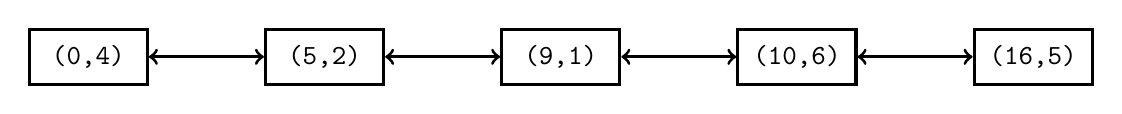
\begin{tikzpicture}

\draw (0.75, 0.35)
  node[draw, line width=0.04cm, , color=black,
       rounded corners=0cm, inner sep=0cm] {

\begin{minipage}[t][0.7cm]{1.5cm}
\mbox{}

\end{minipage}

};\draw (0.75, 0.35) node[color=black] {{\texttt{(0,4)}}};
\draw (3.75, 0.35)
  node[draw, line width=0.04cm, , color=black,
       rounded corners=0cm, inner sep=0cm] {

\begin{minipage}[t][0.7cm]{1.5cm}
\mbox{}

\end{minipage}

};\draw (3.75, 0.35) node[color=black] {{\texttt{(5,2)}}};
\draw (6.75, 0.35)
  node[draw, line width=0.04cm, , color=black,
       rounded corners=0cm, inner sep=0cm] {

\begin{minipage}[t][0.7cm]{1.5cm}
\mbox{}

\end{minipage}

};\draw (6.75, 0.35) node[color=black] {{\texttt{(9,1)}}};
\draw (9.75, 0.35)
  node[draw, line width=0.04cm, , color=black,
       rounded corners=0cm, inner sep=0cm] {

\begin{minipage}[t][0.7cm]{1.5cm}
\mbox{}

\end{minipage}

};\draw (9.75, 0.35) node[color=black] {{\texttt{(10,6)}}};
\draw (12.75, 0.35)
  node[draw, line width=0.04cm, , color=black,
       rounded corners=0cm, inner sep=0cm] {

\begin{minipage}[t][0.7cm]{1.5cm}
\mbox{}

\end{minipage}

};\draw (12.75, 0.35) node[color=black] {{\texttt{(16,5)}}};\draw[line width=0.04cm,black,<->] (1.52,0.35) to  (2.98,0.35);
\draw[line width=0.04cm,black,<->] (4.52,0.35) to  (5.98,0.35);
\draw[line width=0.04cm,black,<->] (7.52,0.35) to  (8.98,0.35);
\draw[line width=0.04cm,black,<->] (10.52,0.35) to  (11.98,0.35);
\end{tikzpicture}

\end{center}



Of course if you perform an infix traversal of a BST and print the
nodes that you visit during the traversal, you will get an ascending
sequence of values taken from tree.


\begin{ex}
How many ways are there to build a BST given
\begin{tightlist}
  \li 2 key values?
  \li 3 key values?
  \li 4 key values?
\end{tightlist}
\qed
\end{ex}
  
\newpage
\subsection{Search}

The point of the BST is to aid in search.
For instance if you're search for \verb!17!, 
you start at the root and see the value \verb!10!.
Since the tree is a BST and you're looking for \verb!17!,
then if it's in the tree, it must be in the right subtree at \verb!10!.
Following the right subtree, we arrive at teh node with value \verb!18!.
Since 17 is less than 18, we follow the left subtree and arrive at 
\verb!15!.
Then following the right subtree, we arrive at \verb!17!.

Of course in this case the number of steps needed is the height of three.

Recall that if $n$ is the number of nodes in a BST
and suppose the height is $h$.
From
\[
h + 1 \leq n \leq 2^{h+1} - 1
\]
we see that 
if the tree has roughly the same number of nodes on the right 
as on the left for each node, i.e., when the tree is balanced. 
the search 
takes
\[
n = 2^{h + 1}
\]
i..e, 
\[
h + 1 = \lg n
\]
In the worst case search when
we see that the number of steps to search for a value is
\[
h + 1 = n 
\]
steps for instance when the BST looks like this

\begin{center}
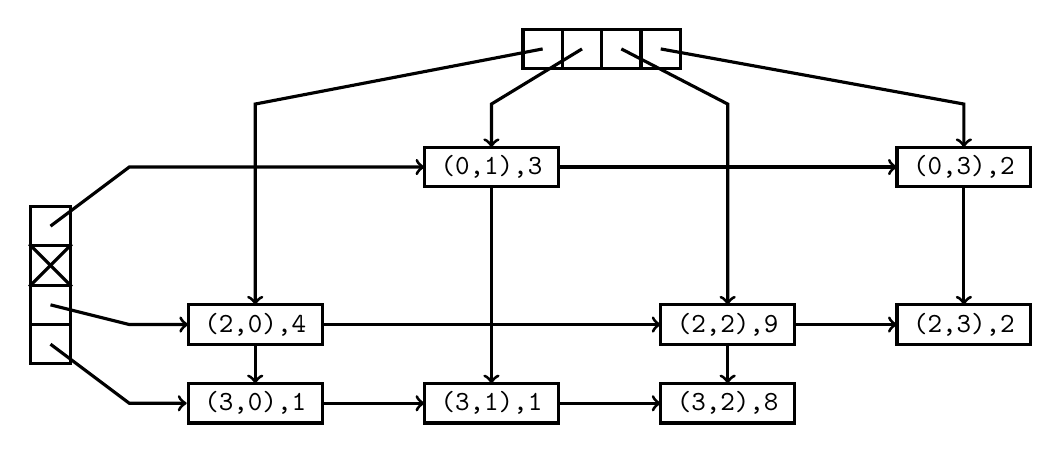
\begin{tikzpicture}

\draw (3.8499999999999996, 3.25)
  node[draw, line width=0.04cm, , color=black,
       rounded corners=0cm, inner sep=0cm] {

\begin{minipage}[t][0.5cm]{1.7cm}
\mbox{}

\end{minipage}

};\draw (3.8499999999999996, 3.25) node[color=black] {{\texttt{(0,1),3}}};
\draw (9.85, 3.25)
  node[draw, line width=0.04cm, , color=black,
       rounded corners=0cm, inner sep=0cm] {

\begin{minipage}[t][0.5cm]{1.7cm}
\mbox{}

\end{minipage}

};\draw (9.85, 3.25) node[color=black] {{\texttt{(0,3),2}}};
\draw (0.85, 1.25)
  node[draw, line width=0.04cm, , color=black,
       rounded corners=0cm, inner sep=0cm] {

\begin{minipage}[t][0.5cm]{1.7cm}
\mbox{}

\end{minipage}

};\draw (0.85, 1.25) node[color=black] {{\texttt{(2,0),4}}};
\draw (6.85, 1.25)
  node[draw, line width=0.04cm, , color=black,
       rounded corners=0cm, inner sep=0cm] {

\begin{minipage}[t][0.5cm]{1.7cm}
\mbox{}

\end{minipage}

};\draw (6.85, 1.25) node[color=black] {{\texttt{(2,2),9}}};
\draw (9.85, 1.25)
  node[draw, line width=0.04cm, , color=black,
       rounded corners=0cm, inner sep=0cm] {

\begin{minipage}[t][0.5cm]{1.7cm}
\mbox{}

\end{minipage}

};\draw (9.85, 1.25) node[color=black] {{\texttt{(2,3),2}}};
\draw (0.85, 0.25)
  node[draw, line width=0.04cm, , color=black,
       rounded corners=0cm, inner sep=0cm] {

\begin{minipage}[t][0.5cm]{1.7cm}
\mbox{}

\end{minipage}

};\draw (0.85, 0.25) node[color=black] {{\texttt{(3,0),1}}};
\draw (3.8499999999999996, 0.25)
  node[draw, line width=0.04cm, , color=black,
       rounded corners=0cm, inner sep=0cm] {

\begin{minipage}[t][0.5cm]{1.7cm}
\mbox{}

\end{minipage}

};\draw (3.8499999999999996, 0.25) node[color=black] {{\texttt{(3,1),1}}};
\draw (6.85, 0.25)
  node[draw, line width=0.04cm, , color=black,
       rounded corners=0cm, inner sep=0cm] {

\begin{minipage}[t][0.5cm]{1.7cm}
\mbox{}

\end{minipage}

};\draw (6.85, 0.25) node[color=black] {{\texttt{(3,2),8}}};\draw[line width=0.04cm,black,->] (4.7,3.25) to  (9,3.25);
\draw[line width=0.04cm,black,->] (7.7,1.25) to  (9,1.25);
\draw[line width=0.04cm,black,->] (1.7,0.25) to  (3,0.25);
\draw[line width=0.04cm,black,->] (4.7,0.25) to  (6,0.25);
\draw[line width=0.04cm,black,->] (3.85,3) to  (3.85,0.5);
\draw[line width=0.04cm,black,->] (6.85,1) to  (6.85,0.5);
\draw[line width=0.04cm,black,->] (9.85,3) to  (9.85,1.5);
\draw[line width=0.04cm,black,->] (1.7,1.25) to  (6,1.25);
\draw[line width=0.04cm,black,->] (0.85,1) to  (0.85,0.5);

\draw (-1.75, 2.5)
  node[draw, line width=0.04cm, , color=black,
       rounded corners=0cm, inner sep=0cm] {

\begin{minipage}[t][0.5cm]{0.5cm}
\mbox{}

\end{minipage}

};
\draw (-1.75, 2.0)
  node[draw, line width=0.04cm, , color=black,
       rounded corners=0cm, inner sep=0cm] {

\begin{minipage}[t][0.5cm]{0.5cm}
\mbox{}

\end{minipage}

};
\draw (-1.75, 1.5)
  node[draw, line width=0.04cm, , color=black,
       rounded corners=0cm, inner sep=0cm] {

\begin{minipage}[t][0.5cm]{0.5cm}
\mbox{}

\end{minipage}

};
\draw (-1.75, 1.0)
  node[draw, line width=0.04cm, , color=black,
       rounded corners=0cm, inner sep=0cm] {

\begin{minipage}[t][0.5cm]{0.5cm}
\mbox{}

\end{minipage}

};\draw[line width=0.04cm,black,->] (-1.75,2.5) to  (-0.75,3.25) to  (3,3.25);
\draw[line width=0.04cm,black] (-2.02,2.27) to  (-1.48,1.73);
\draw[line width=0.04cm,black] (-1.48,2.27) to  (-2.02,1.73);
\draw[line width=0.04cm,black,->] (-1.75,1.5) to  (-0.75,1.25) to  (0,1.25);
\draw[line width=0.04cm,black,->] (-1.75,1.0) to  (-0.75,0.25) to  (-0.02,0.25);

\draw (4.5, 4.75)
  node[draw, line width=0.04cm, , color=black,
       rounded corners=0cm, inner sep=0cm] {

\begin{minipage}[t][0.5cm]{0.5cm}
\mbox{}

\end{minipage}

};
\draw (5.0, 4.75)
  node[draw, line width=0.04cm, , color=black,
       rounded corners=0cm, inner sep=0cm] {

\begin{minipage}[t][0.5cm]{0.5cm}
\mbox{}

\end{minipage}

};
\draw (5.5, 4.75)
  node[draw, line width=0.04cm, , color=black,
       rounded corners=0cm, inner sep=0cm] {

\begin{minipage}[t][0.5cm]{0.5cm}
\mbox{}

\end{minipage}

};
\draw (6.0, 4.75)
  node[draw, line width=0.04cm, , color=black,
       rounded corners=0cm, inner sep=0cm] {

\begin{minipage}[t][0.5cm]{0.5cm}
\mbox{}

\end{minipage}

};\draw[line width=0.04cm,black,->] (4.5,4.75) to  (0.85,4.05) to  (0.85,1.5);
\draw[line width=0.04cm,black,->] (5.0,4.75) to  (3.85,4.05) to  (3.85,3.5);
\draw[line width=0.04cm,black,->] (5.5,4.75) to  (6.85,4.05) to  (6.85,1.5);
\draw[line width=0.04cm,black,->] (6.0,4.75) to  (9.85,4.05) to  (9.85,3.5);
\end{tikzpicture}

\end{center}



This is the worst case, i.e., the worst runtime for BST search is
\[
O(n)
\]
The point is that if the tree is heavily \lq\lq unbalanced'',
i.e., all the nodes are always \lq\lq on the left'' or \lq\lq on the right''.
In the average case,
the BST is \lq\lq roughly'' balanced and therefore
the average runtime for BST search is
\[
O(\log n)
\]


\newpage
\begin{ex}
  
  Given this BST
  
\begin{center}

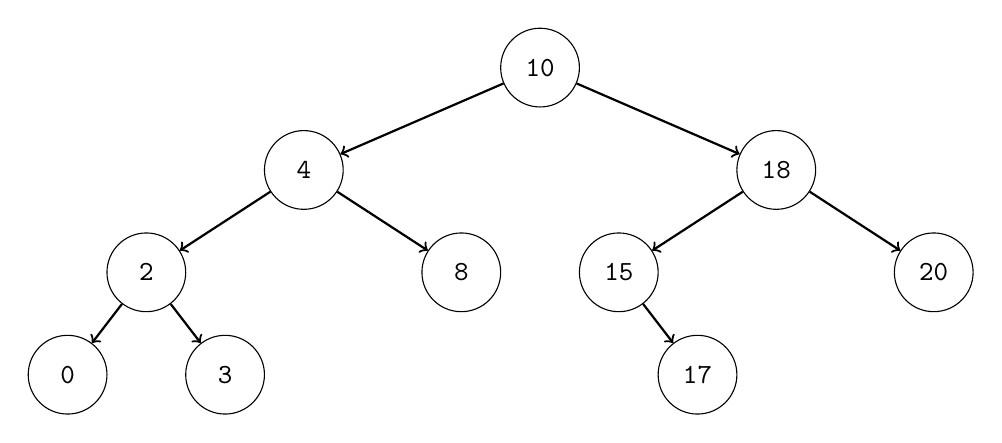
\begin{tikzpicture}
\node at (6,-1.3) [circle,draw,minimum size=10mm] (a) {\texttt{10}};
\node at (3,-2.6) [circle,draw,minimum size=10mm] (b) {\texttt{4}};
\node at (9,-2.6) [circle,draw,minimum size=10mm] (d) {\texttt{18}};
\node at (1,-3.9000000000000004) [circle,draw,minimum size=10mm] (e) {\texttt{2}};
\node at (5,-3.9000000000000004) [circle,draw,minimum size=10mm] (f) {\texttt{8}};
\node at (7,-3.9000000000000004) [circle,draw,minimum size=10mm] (h) {\texttt{15}};
\node at (11,-3.9000000000000004) [circle,draw,minimum size=10mm] (j) {\texttt{20}};
\node at (0,-5.2) [circle,draw,minimum size=10mm] (k) {\texttt{0}};
\node at (2,-5.2) [circle,draw,minimum size=10mm] (l) {\texttt{3}};
\node at (8,-5.2) [circle,draw,minimum size=10mm] (m) {\texttt{17}};
\draw [->,thick] (a) -- (b);
\draw [->,thick] (a) -- (d);
\draw [->,thick] (b) -- (e);
\draw [->,thick] (b) -- (f);
\draw [->,thick] (d) -- (h);
\draw [->,thick] (d) -- (j);
\draw [->,thick] (e) -- (k);
\draw [->,thick] (e) -- (l);
\draw [->,thick] (h) -- (m);

;
\end{tikzpicture}
    
\end{center}


what nodes were visited while performing a BST search for
the following cases: 4, 9, 20?
\qed
\end{ex}


\newpage
Here's the algorithm to perform a search in a BST:
\begin{console}
ALGORITHM: BST-SEARCH
INPUT: node
       key (the target)

if node is NONE:
    return NOT FOUND

if node.key is key:
    return node
else:
    if key < node.key:
        BST-SEARCH(node.left, key)
    else data > node.data:
        BST-SEARCH(node.right, key)
\end{console}

Here's a version that's close to C++:
\begin{console}
Node * bst_search(Node * p, int key)
{
    if p is NULL, return NULL

    if p->key is key
        return p
    else if key < p->key
        bst_search(p->left, key)
    else key > p->key
        bst_search(p->right, key)
}
\end{console}


\newpage
\begin{ex}
Implement the following
C++ function so that it performs a BST search
and returns the pointer to the node with the
given key value; \verb!NULL! is returned is the
key value is not found in the BST.
\begin{Verbatim}[frame=single]
Node * bst_search(Node * p, int key);
\end{Verbatim}
\end{ex}




\newpage
\subsection{Insert}

Of course when you insert a value into a BST, 
you have to make sure it's still a BST so that search for it
later is still fast.
Note that a BST is a self-organizing container.

\begin{console}
ALGORITHM: BST-INSERT
INPUT: node
       newvalue

if node is NONE:
    set node to a new node with key newvalue
    return
 
if node.key < newvalue:
    if node.right is NONE:
        create a new node with key newvalue and
        make it the left child of node
    else:
        BST-INSERT(node.right, newvalue)
else if node.key > newvalue:
    if node.left is NONE:
        create a new node with key newvalue and
        make it the right child of node
    else:
        BST-INSERT(node.left, newvalue)
else:
    return ERROR -- DUPLICATE NODE
\end{console}

The runtime behavior is similar to the runtime behavior for
BST search.
The worst case is
\[
O(n)
\]
The average runtime is
\[
O(\log n)
\]

In the above, I'm assuming that the key values in the BST
are unique.

\newpage
\begin{ex}
Now C++ pseudocode this time ... implement the following C++ functions
\begin{Verbatim}[frame=single]
void bst_insert(Node ** p, int key);
void bst_insert(Node *& p, int key);
\end{Verbatim}
(Just for practice, throw an exception when there's a duplicate key.)
\qed
\end{ex}


\newpage
\begin{ex}
The above algorithms are rather similar.
Can you find a useful helper function?
(Instead of a pointer \verb!q! walking down the tree, you need another
pointer \verb!r! that is \lq\lq behind'' \verb!q!.)
\qed
\end{ex}

\newpage
\subsection{Delete}

But what about node deletion?
No problem when deleting leaves of course.
What about deleting a non-leaf node?
Look at this again:


\begin{center}
\begin{tikzpicture}[>=triangle 60,shorten >=0.5pt,node distance=2cm,auto,initial text=, double distance=2pt]
\node[state] (A) at (  0,  0) {$0$};
\node[state] (B) at (  3,  0) {$1$};
\node[state] (F) at (  6,  0) {$2$};
\node[state] (C) at (  0, -2) {$3$};
\node[state] (D) at (  3, -2) {$4$};
\node[state] (E) at (  6, -2) {$5$};

\path[->]
(A) edge [loop above] node {} ()
(A) edge [bend left=0,pos=0.5,above] node {} (B)
(B) edge [bend left=0,pos=0.5] node {} (D)
(B) edge [bend left=0,pos=0.5,above] node {} (E)
(C) edge [bend left=0,pos=0.5,above] node {} (B)
(C) edge [bend left=0,pos=0.5,above] node {} (D)
(D) edge [bend left=0,pos=0.5,above] node {} (E)

;
\end{tikzpicture}
\end{center}
    


If I delete \verb!4!, maybe we can move \verb!8! up to occupy
the position taken up by \verb!4!:
\begin{center}
\begin{tikzpicture}

\fill[white] (18.0, -2.0) circle (0.3);
\node [line width=0.03cm,black,minimum size=0.57cm,draw,circle] at (18.0,-2.0)(A){};\draw (18.0, -2.0) node[color=black] {\texttt{20}};
\fill[white] (13.0, 0.0) circle (0.3);
\node [line width=0.03cm,black,minimum size=0.57cm,draw,circle] at (13.0,0.0)(a){};\draw (13.0, 0.0) node[color=black] {\texttt{10}};
\fill[white] (10.0, -1.0) circle (0.3);
\node [line width=0.03cm,black,minimum size=0.57cm,draw,circle] at (10.0,-1.0)(b){};\draw (10.0, -1.0) node[color=black] {\texttt{8}};
\fill[white] (16.0, -1.0) circle (0.3);
\node [line width=0.03cm,black,minimum size=0.57cm,draw,circle] at (16.0,-1.0)(p){};\draw (16.0, -1.0) node[color=black] {\texttt{18}};
\fill[white] (8.0, -2.0) circle (0.3);
\node [line width=0.03cm,black,minimum size=0.57cm,draw,circle] at (8.0,-2.0)(e){};\draw (8.0, -2.0) node[color=black] {\texttt{2}};
\fill[white] (7.0, -3.0) circle (0.3);
\node [line width=0.03cm,black,minimum size=0.57cm,draw,circle] at (7.0,-3.0)(k){};\draw (7.0, -3.0) node[color=black] {\texttt{0}};
\fill[white] (9.0, -3.0) circle (0.3);
\node [line width=0.03cm,black,minimum size=0.57cm,draw,circle] at (9.0,-3.0)(l){};\draw (9.0, -3.0) node[color=black] {\texttt{3}};
\fill[white] (14.0, -2.0) circle (0.3);
\node [line width=0.03cm,black,minimum size=0.57cm,draw,circle] at (14.0,-2.0)(h){};\draw (14.0, -2.0) node[color=black] {\texttt{15}};
\fill[white] (15.0, -3.0) circle (0.3);
\node [line width=0.03cm,black,minimum size=0.57cm,draw,circle] at (15.0,-3.0)(m){};\draw (15.0, -3.0) node[color=black] {\texttt{17}};\draw[line width=0.03cm,black,->,>=triangle 60] (a) to  (p);
\draw[line width=0.03cm,black,->,>=triangle 60] (h) to  (m);
\draw[line width=0.03cm,black,->,>=triangle 60] (a) to  (b);
\draw[line width=0.03cm,black,->,>=triangle 60] (p) to  (h);
\draw[line width=0.03cm,black,->,>=triangle 60] (p) to  (A);
\draw[line width=0.03cm,black,->,>=triangle 60] (b) to  (e);
\draw[line width=0.03cm,black,->,>=triangle 60] (e) to  (k);
\draw[line width=0.03cm,black,->,>=triangle 60] (e) to  (l);
\end{tikzpicture}

\end{center}


Why is that possible?
Because \verb!8! has no left child.
If \verb!8! has a left child, when you move \verb!8! up,
its left child will \lq\lq collide'' with \verb!2!.
Right?
Think about this:
if \verb!8! has a right child (or even a right subtree) but no 
left child,
you can \textit{still} move \verb!8! up to \verb!4!'s place.

But what if I want to move something up from the left of \verb!4!?
For instance, remember that we do want our BSTs to be
as balanced as possible. 
Since there are more node on the left of \verb!4!,
maybe we want to move something on the left of \verb!4! up
to \verb!4!'s position instead of using some node on the 
right. How are we going to do that???

Furthermore, what if I need to delete \verb!10!?
You see that it's not so clear what we should do ...

You can of course do an inorder traversal of the tree
to create an array/vector/list of the nodes, omitting \verb!10!,
and then rebuild the tree.
But that's extremely costly!!!
We want to disrupt the tree minimally!!!

If you think about it, you see that
to delete root \verb!10!,
you want to you can move the \verb!8! to the 
same place as the root
or move \texttt{15} to the root's place.
Why?
Two reasons:
because they have at most
one child and because they are values closest to 
\verb!10!!!!
The fact that they have at most one child
means that their single child can move to their place without
worry about collisions when they are moved to their new places.
For instance, see \texttt{17} the right child of \texttt{15} above.
The fact that they are values closest to \verb!10! means that
there won't be nodes between them and \verb!10! that might be
disrupted because of the move.
Right?

In the case of moving \verb!8!, we get this
\begin{center}
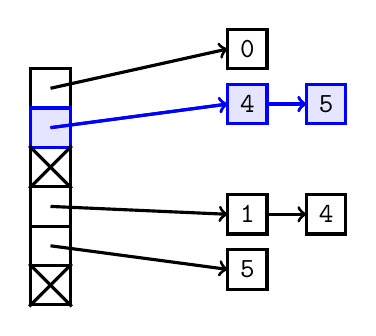
\begin{tikzpicture}

\draw (0.25, -0.25)
  node[draw, line width=0.04cm, , color=black,
       rounded corners=0cm, inner sep=0cm] {

\begin{minipage}[t][0.5cm]{0.5cm}
\mbox{}

\end{minipage}

};
\draw (0.25, -0.75)
  node[fill=blue!10,rounded corners=0cm,inner sep=0cm] {

\begin{minipage}[t][0.5cm]{0.5cm}
\mbox{}

\end{minipage}

};
\draw (0.25, -0.75)
  node[draw, line width=0.04cm, , color=blue,
       rounded corners=0cm, inner sep=0cm] {

\begin{minipage}[t][0.5cm]{0.5cm}
\mbox{}

\end{minipage}

};
\draw (0.25, -1.25)
  node[draw, line width=0.04cm, , color=black,
       rounded corners=0cm, inner sep=0cm] {

\begin{minipage}[t][0.5cm]{0.5cm}
\mbox{}

\end{minipage}

};
\draw (0.25, -1.75)
  node[draw, line width=0.04cm, , color=black,
       rounded corners=0cm, inner sep=0cm] {

\begin{minipage}[t][0.5cm]{0.5cm}
\mbox{}

\end{minipage}

};
\draw (0.25, -2.25)
  node[draw, line width=0.04cm, , color=black,
       rounded corners=0cm, inner sep=0cm] {

\begin{minipage}[t][0.5cm]{0.5cm}
\mbox{}

\end{minipage}

};
\draw (0.25, -2.75)
  node[draw, line width=0.04cm, , color=black,
       rounded corners=0cm, inner sep=0cm] {

\begin{minipage}[t][0.5cm]{0.5cm}
\mbox{}

\end{minipage}

};
\draw (0.25, -0.75)
  node[fill=blue!10,rounded corners=0cm,inner sep=0cm] {

\begin{minipage}[t][0.5cm]{0.5cm}
\mbox{}

\end{minipage}

};
\draw (0.25, -0.75)
  node[draw, line width=0.04cm, , color=blue,
       rounded corners=0cm, inner sep=0cm] {

\begin{minipage}[t][0.5cm]{0.5cm}
\mbox{}

\end{minipage}

};\draw[line width=0.04cm,black] (-0.02,-0.98) to  (0.52,-1.52);
\draw[line width=0.04cm,black] (0.52,-0.98) to  (-0.02,-1.52);
\draw[line width=0.04cm,black] (-0.02,-2.48) to  (0.52,-3.02);
\draw[line width=0.04cm,black] (0.52,-2.48) to  (-0.02,-3.02);

\draw (2.75, 0.24999999999999992)
  node[draw, line width=0.04cm, , color=black,
       rounded corners=0cm, inner sep=0cm] {

\begin{minipage}[t][0.5cm]{0.5cm}
\mbox{}

\end{minipage}

};\draw (2.75, 0.24999999999999992) node[color=black] {{\texttt{0}}};
\draw (2.75, -0.45000000000000007)
  node[fill=blue!10,rounded corners=0cm,inner sep=0cm] {

\begin{minipage}[t][0.5cm]{0.5cm}
\mbox{}

\end{minipage}

};
\draw (2.75, -0.45000000000000007)
  node[draw, line width=0.04cm, , color=blue,
       rounded corners=0cm, inner sep=0cm] {

\begin{minipage}[t][0.5cm]{0.5cm}
\mbox{}

\end{minipage}

};\draw (2.75, -0.45000000000000007) node[color=black] {{\texttt{4}}};
\draw (3.75, -0.45000000000000007)
  node[fill=blue!10,rounded corners=0cm,inner sep=0cm] {

\begin{minipage}[t][0.5cm]{0.5cm}
\mbox{}

\end{minipage}

};
\draw (3.75, -0.45000000000000007)
  node[draw, line width=0.04cm, , color=blue,
       rounded corners=0cm, inner sep=0cm] {

\begin{minipage}[t][0.5cm]{0.5cm}
\mbox{}

\end{minipage}

};\draw (3.75, -0.45000000000000007) node[color=black] {{\texttt{5}}};
\draw (2.75, -1.85)
  node[draw, line width=0.04cm, , color=black,
       rounded corners=0cm, inner sep=0cm] {

\begin{minipage}[t][0.5cm]{0.5cm}
\mbox{}

\end{minipage}

};\draw (2.75, -1.85) node[color=black] {{\texttt{1}}};
\draw (3.75, -1.85)
  node[draw, line width=0.04cm, , color=black,
       rounded corners=0cm, inner sep=0cm] {

\begin{minipage}[t][0.5cm]{0.5cm}
\mbox{}

\end{minipage}

};\draw (3.75, -1.85) node[color=black] {{\texttt{4}}};
\draw (2.75, -2.55)
  node[draw, line width=0.04cm, , color=black,
       rounded corners=0cm, inner sep=0cm] {

\begin{minipage}[t][0.5cm]{0.5cm}
\mbox{}

\end{minipage}

};\draw (2.75, -2.55) node[color=black] {{\texttt{5}}};
\draw (2.75, -0.45000000000000007)
  node[fill=blue!10,rounded corners=0cm,inner sep=0cm] {

\begin{minipage}[t][0.5cm]{0.5cm}
\mbox{}

\end{minipage}

};
\draw (2.75, -0.45000000000000007)
  node[draw, line width=0.04cm, , color=blue,
       rounded corners=0cm, inner sep=0cm] {

\begin{minipage}[t][0.5cm]{0.5cm}
\mbox{}

\end{minipage}

};\draw (2.75, -0.45000000000000007) node[color=black] {{\texttt{4}}};
\draw (3.75, -0.45000000000000007)
  node[fill=blue!10,rounded corners=0cm,inner sep=0cm] {

\begin{minipage}[t][0.5cm]{0.5cm}
\mbox{}

\end{minipage}

};
\draw (3.75, -0.45000000000000007)
  node[draw, line width=0.04cm, , color=blue,
       rounded corners=0cm, inner sep=0cm] {

\begin{minipage}[t][0.5cm]{0.5cm}
\mbox{}

\end{minipage}

};\draw (3.75, -0.45000000000000007) node[color=black] {{\texttt{5}}};\draw[line width=0.04cm,black,->] (0.25,-0.25) to  (2.5,0.25);
\draw[line width=0.04cm,blue,->] (0.25,-0.75) to  (2.5,-0.45);
\draw[line width=0.04cm,blue,->] (3.0,-0.45) to  (3.5,-0.45);
\draw[line width=0.04cm,black,->] (0.25,-1.75) to  (2.5,-1.85);
\draw[line width=0.04cm,black,->] (3.0,-1.85) to  (3.5,-1.85);
\draw[line width=0.04cm,black,->] (0.25,-2.25) to  (2.5,-2.55);
\draw[line width=0.04cm,blue,->] (0.25,-0.75) to  (2.5,-0.45);
\draw[line width=0.04cm,blue,->] (3.0,-0.45) to  (3.5,-0.45);
\end{tikzpicture}

\end{center}



and in the case of moving \texttt{15}, we get this:
\input{stdout41.tex}

In the second case, the value that is moved, i.e. \texttt{15},
has a right child \texttt{17} which becomes the left child of \verb!18!.

Specifically, the value that is moved up to the root
is the rightmost of the left subtree
or the leftmost of the right subtree.
\verb!8! (or the node with \verb!8!)
is called the \defone{predecessor} of the node with value \verb!10!
and the node with \texttt{15} is the 
\defone{successor} of the node with value \verb!10!.

The algorithm for the predecessor is easy: take one
left step and take as many right steps as you can:
\begin{console}
// bst_predecessor of p
if p is NULL:
    return NULL
else:
    let q = p->left_
    while q is not NULL:
        q = q->NULL
    return q
\end{console}
I'll leave it to you to write \verb!bst_sucessor! function.

Clearly, since \verb!8! is the rightmost of the 
left subtree at \verb!4!,
it is also the largest value in this left subtree.
Therefore moving it to the root
will preserve the ordering requirement for a BST.
Similarly, moving the leftmost of the right subtree at \verb!18!
will preserve the BST property.

There are several details to consider.
Consider the following bst where we want to delete 10:
\begin{center}
\begin{tikzpicture}

\fill[white] (19.0, -0.6) circle (0.3);
\node [line width=0.03cm,black,minimum size=0.57cm,draw,circle] at (19.0,-0.6)(A){};\draw (19.0, -0.6) node[color=black] {\texttt{20}};
\fill[white] (16.0, -1.0) circle (0.3);
\node [line width=0.03cm,black,minimum size=0.57cm,draw,circle] at (16.0,-1.0)(a){};\draw (16.0, -1.0) node[color=black] {\texttt{10}};
\fill[white] (10.0, -2.0) circle (0.3);
\node [line width=0.03cm,black,minimum size=0.57cm,draw,circle] at (10.0,-2.0)(b){};\draw (10.0, -2.0) node[color=black] {\texttt{0}};
\fill[white] (11.0, -4.0) circle (0.3);
\node [line width=0.03cm,black,minimum size=0.57cm,draw,circle] at (11.0,-4.0)(d){};\draw (11.0, -4.0) node[color=black] {\texttt{18}};
\fill[white] (8.0, -3.0) circle (0.3);
\node [line width=0.03cm,black,minimum size=0.57cm,draw,circle] at (8.0,-3.0)(e){};\draw (8.0, -3.0) node[color=black] {\texttt{-2}};
\fill[white] (7.0, -4.0) circle (0.3);
\node [line width=0.03cm,black,minimum size=0.57cm,draw,circle] at (7.0,-4.0)(k){};\draw (7.0, -4.0) node[color=black] {\texttt{-3}};
\fill[white] (9.0, -4.0) circle (0.3);
\node [line width=0.03cm,black,minimum size=0.57cm,draw,circle] at (9.0,-4.0)(l){};\draw (9.0, -4.0) node[color=black] {\texttt{-1}};
\fill[white] (15.0, -4.0) circle (0.3);
\node [line width=0.03cm,black,minimum size=0.57cm,draw,circle] at (15.0,-4.0)(h){};\draw (15.0, -4.0) node[color=black] {\texttt{8}};
\fill[white] (14.0, -5.0) circle (0.3);
\node [line width=0.03cm,black,minimum size=0.57cm,draw,circle] at (14.0,-5.0)(m){};\draw (14.0, -5.0) node[color=black] {\texttt{6}};
\fill[white] (13.0, -3.0) circle (0.3);
\node [line width=0.03cm,black,minimum size=0.57cm,draw,circle] at (13.0,-3.0)(f){};\draw (13.0, -3.0) node[color=black] {\texttt{5}};
\fill[white] (13.0, -6.0) circle (0.3);
\node [line width=0.03cm,black,minimum size=0.57cm,draw,circle] at (13.0,-6.0)(n){};\draw (13.0, -6.0) node[color=black] {\texttt{4}};
\fill[white] (15.0, -6.0) circle (0.3);
\node [line width=0.03cm,black,minimum size=0.57cm,draw,circle] at (15.0,-6.0)(o){};\draw (15.0, -6.0) node[color=black] {\texttt{7}};
\fill[white] (18.0, -2.0) circle (0.3);
\node [line width=0.03cm,black,minimum size=0.57cm,draw,circle] at (18.0,-2.0)(p){};\draw (18.0, -2.0) node[color=black] {\texttt{15}};\draw[line width=0.03cm,black,->,>=triangle 60] (A) to  (a);
\draw[line width=0.03cm,black,->,>=triangle 60] (a) to  (p);
\draw[line width=0.03cm,black,->,>=triangle 60] (a) to  (b);
\draw[line width=0.03cm,black,->,>=triangle 60] (b) to  (e);
\draw[line width=0.03cm,black,->,>=triangle 60] (b) to  (f);
\draw[line width=0.03cm,black,->,>=triangle 60] (f) to  (d);
\draw[line width=0.03cm,black,->,>=triangle 60] (f) to  (h);
\draw[line width=0.03cm,black,->,>=triangle 60] (e) to  (k);
\draw[line width=0.03cm,black,->,>=triangle 60] (e) to  (l);
\draw[line width=0.03cm,black,->,>=triangle 60] (h) to  (m);
\draw[line width=0.03cm,black,->,>=triangle 60] (m) to  (n);
\draw[line width=0.03cm,black,->,>=triangle 60] (m) to  (o);
\end{tikzpicture}

\end{center}



(the same idea below applies to the right of 10 if 10
has a right child but no left child.)

\textsc{Method 1}.
We just copy 8 to 10, 
link the right pointer of 5 to 6, and then
deallocate 8:
from latextool_basic import *
print(automata(layout="""
A  B

C  D
""",
edges="A,$a$,B|A,$b$,C|B,$a$,D|B,$b$,C|C,$b$,A|C,$a$,D|D,$a$,B|D,$b$,A",
A='initial|label=$q_0$',
B='accept|label=$q_1$',
C='label=$q_2$',
D='accept|label=$q_3$', xscale=1.3,
))

Suppose \verb!p! points to the node to be deleted and
\verb!q! points to the predecessor.
The above is
\begin{console}
// move-predecessor-up algorithm
q->parent_->right_ = q->left_ // point 5 to 6
p->key_ = q->key_             // move 8 up to 10
delete q
\end{console}



\begin{ex}
  Note that in the above code we used \verb!->! in
  several places.
  Can we do that?
  For instance we used \verb!q->parent_! -- can we do that?
  For instance we used \verb!q->parent_->right_!: can we do that?
\end{ex}


\begin{ex}
What if the node with 0 is in fact the predecessor?
(i.e., assume the left pointer of the node with 0 is NULL).
In other words, in the algorithm above, at \verb!p!,
we take one left step and then as many right steps as we can.
What if after a left step, we cannot take any right step at all?
Here's the picture for this case:
\begin{center}
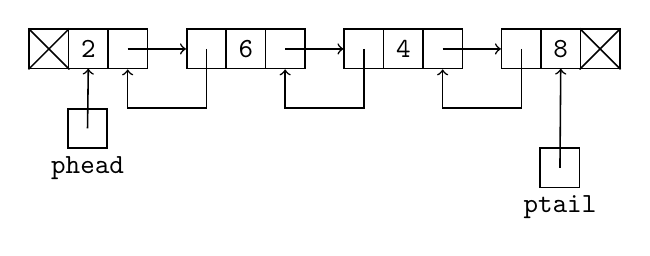
\begin{tikzpicture}

\draw (0.25, 0.25)
  node[draw, line width=0.02cm, , color=black,
       rounded corners=0cm, inner sep=0cm] {

\begin{minipage}[t][0.5cm]{0.5cm}
\mbox{}

\end{minipage}

};\draw (0.25, 0.25) node[color=black] {{\texttt{}}};
\draw (0.75, 0.25)
  node[draw, line width=0.02cm, , color=black,
       rounded corners=0cm, inner sep=0cm] {

\begin{minipage}[t][0.5cm]{0.5cm}
\mbox{}

\end{minipage}

};\draw (0.75, 0.25) node[color=black] {{\texttt{2}}};
\draw (1.25, 0.25)
  node[draw, line width=0.02cm, , color=black,
       rounded corners=0cm, inner sep=0cm] {

\begin{minipage}[t][0.5cm]{0.5cm}
\mbox{}

\end{minipage}

};\draw (1.25, 0.25) node[color=black] {{\texttt{}}};
\draw (2.25, 0.25)
  node[draw, line width=0.02cm, , color=black,
       rounded corners=0cm, inner sep=0cm] {

\begin{minipage}[t][0.5cm]{0.5cm}
\mbox{}

\end{minipage}

};\draw (2.25, 0.25) node[color=black] {{\texttt{}}};
\draw (2.75, 0.25)
  node[draw, line width=0.02cm, , color=black,
       rounded corners=0cm, inner sep=0cm] {

\begin{minipage}[t][0.5cm]{0.5cm}
\mbox{}

\end{minipage}

};\draw (2.75, 0.25) node[color=black] {{\texttt{6}}};
\draw (3.25, 0.25)
  node[draw, line width=0.02cm, , color=black,
       rounded corners=0cm, inner sep=0cm] {

\begin{minipage}[t][0.5cm]{0.5cm}
\mbox{}

\end{minipage}

};\draw (3.25, 0.25) node[color=black] {{\texttt{}}};
\draw (4.25, 0.25)
  node[draw, line width=0.02cm, , color=black,
       rounded corners=0cm, inner sep=0cm] {

\begin{minipage}[t][0.5cm]{0.5cm}
\mbox{}

\end{minipage}

};\draw (4.25, 0.25) node[color=black] {{\texttt{}}};
\draw (4.75, 0.25)
  node[draw, line width=0.02cm, , color=black,
       rounded corners=0cm, inner sep=0cm] {

\begin{minipage}[t][0.5cm]{0.5cm}
\mbox{}

\end{minipage}

};\draw (4.75, 0.25) node[color=black] {{\texttt{4}}};
\draw (5.25, 0.25)
  node[draw, line width=0.02cm, , color=black,
       rounded corners=0cm, inner sep=0cm] {

\begin{minipage}[t][0.5cm]{0.5cm}
\mbox{}

\end{minipage}

};\draw (5.25, 0.25) node[color=black] {{\texttt{}}};
\draw (6.25, 0.25)
  node[draw, line width=0.02cm, , color=black,
       rounded corners=0cm, inner sep=0cm] {

\begin{minipage}[t][0.5cm]{0.5cm}
\mbox{}

\end{minipage}

};\draw (6.25, 0.25) node[color=black] {{\texttt{}}};
\draw (6.75, 0.25)
  node[draw, line width=0.02cm, , color=black,
       rounded corners=0cm, inner sep=0cm] {

\begin{minipage}[t][0.5cm]{0.5cm}
\mbox{}

\end{minipage}

};\draw (6.75, 0.25) node[color=black] {{\texttt{8}}};
\draw (7.25, 0.25)
  node[draw, line width=0.02cm, , color=black,
       rounded corners=0cm, inner sep=0cm] {

\begin{minipage}[t][0.5cm]{0.5cm}
\mbox{}

\end{minipage}

};\draw (7.25, 0.25) node[color=black] {{\texttt{}}};\draw[line width=0.02cm,black,->] (1.25,0.25) to  (1.99,0.25);
\draw[line width=0.02cm,black,->] (3.25,0.25) to  (3.99,0.25);
\draw[line width=0.02cm,black,->] (2.25,0.25) to  (2.25,-0.5) to  (1.25,-0.5) to  (1.25,-0.01);
\draw[line width=0.02cm,black,->] (5.25,0.25) to  (5.99,0.25);
\draw[line width=0.02cm,black,->] (4.25,0.25) to  (4.25,-0.5) to  (3.25,-0.5) to  (3.25,-0.01);
\draw[line width=0.02cm,black,->] (6.25,0.25) to  (6.25,-0.5) to  (5.25,-0.5) to  (5.25,-0.01);
\draw[line width=0.02cm,black] (-0.01,0.51) to  (0.51,-0.01);
\draw[line width=0.02cm,black] (0.51,0.51) to  (-0.01,-0.01);
\draw[line width=0.02cm,black] (6.99,0.51) to  (7.51,-0.01);
\draw[line width=0.02cm,black] (7.51,0.51) to  (6.99,-0.01);

\draw (0.74, -0.76)
  node[draw, line width=0.02cm, , color=black,
       rounded corners=0cm, inner sep=0cm] {

\begin{minipage}[t][0.5cm]{0.5cm}
\mbox{}

\end{minipage}

};\draw (0.74, -0.76) node[color=black] {{\texttt{}}};
\draw (0.74, -1.26)
  node[draw, line width=0.02cm, , color=white,
       rounded corners=0cm, inner sep=0cm] {

\begin{minipage}[t][0.1cm]{0.1cm}
\mbox{}

\end{minipage}

};\draw (0.74, -1.26) node[color=black] {{\texttt{phead}}};\draw[line width=0.02cm,black,->] (0.74,-0.76) to  (0.75,0);

\draw (6.74, -1.26)
  node[draw, line width=0.02cm, , color=black,
       rounded corners=0cm, inner sep=0cm] {

\begin{minipage}[t][0.5cm]{0.5cm}
\mbox{}

\end{minipage}

};\draw (6.74, -1.26) node[color=black] {{\texttt{}}};
\draw (6.74, -1.76)
  node[draw, line width=0.02cm, , color=white,
       rounded corners=0cm, inner sep=0cm] {

\begin{minipage}[t][0.1cm]{0.1cm}
\mbox{}

\end{minipage}

};\draw (6.74, -1.76) node[color=black] {{\texttt{ptail}}};\draw[line width=0.02cm,black,->] (6.74,-1.26) to  (6.75,0);
\end{tikzpicture}

\end{center}


Do you need to change the move-predecessor-up algorithm?
The resulting picture should obviously be this:
\begin{center}
\begin{tikzpicture}

\fill[white] (19.0, -0.6) circle (0.3);
\node [line width=0.03cm,black,minimum size=0.57cm,draw,circle] at (19.0,-0.6)(A){};\draw (19.0, -0.6) node[color=black] {\texttt{20}};
\fill[white] (16.0, -1.0) circle (0.3);
\node [line width=0.03cm,black,minimum size=0.57cm,draw,circle] at (16.0,-1.0)(a){};\draw (16.0, -1.0) node[color=black] {\texttt{10}};\draw[line width=0.1cm,black] (15.8,-1.2) to  (16.2,-0.8);

\fill[white] (16.0, -2.0) circle (0.3);
\node [line width=0.03cm,white,minimum size=0.57cm,draw,circle] at (16.0,-2.0)(aa){};\draw (16.0, -2.0) node[color=black] {\texttt{0}};\draw[line width=0.05cm,black,->,>=triangle 60] (aa) to  (a);

\fill[white] (10.0, -2.0) circle (0.3);
\node [line width=0.03cm,black,,dashed,minimum size=0.57cm,draw,circle] at (10.0,-2.0)(b){};\draw (10.0, -2.0) node[color=black] {\texttt{0}};
\fill[white] (8.0, -3.0) circle (0.3);
\node [line width=0.03cm,black,minimum size=0.57cm,draw,circle] at (8.0,-3.0)(e){};\draw (8.0, -3.0) node[color=black] {\texttt{-2}};
\fill[white] (7.0, -4.0) circle (0.3);
\node [line width=0.03cm,black,minimum size=0.57cm,draw,circle] at (7.0,-4.0)(k){};\draw (7.0, -4.0) node[color=black] {\texttt{-3}};
\fill[white] (9.0, -4.0) circle (0.3);
\node [line width=0.03cm,black,minimum size=0.57cm,draw,circle] at (9.0,-4.0)(l){};\draw (9.0, -4.0) node[color=black] {\texttt{-1}};
\fill[white] (18.0, -2.0) circle (0.3);
\node [line width=0.03cm,black,minimum size=0.57cm,draw,circle] at (18.0,-2.0)(p){};\draw (18.0, -2.0) node[color=black] {\texttt{15}};\draw[line width=0.03cm,black,->,>=triangle 60] (a) to  (e);
\draw[line width=0.03cm,black,->,>=triangle 60] (A) to  (a);
\draw[line width=0.03cm,black,->,>=triangle 60] (a) to  (p);
\draw[line width=0.03cm,black,->,>=triangle 60] (e) to  (k);
\draw[line width=0.03cm,black,->,>=triangle 60] (e) to  (l);
\draw[line width=0.03cm,black,->,>=triangle 60,dashed] (a) to  (b);
\draw[line width=0.03cm,black,->,>=triangle 60,dashed] (b) to  (e);
\end{tikzpicture}

\end{center}


\begin{console}[commandchars=\\\{\}]
// move-predecessor-up algorithm
if q is not p->left_:
    q->parent_->right_ = q->left_ 
    p->key_ = q->key_             
    delete q
else:
    \textwhite{p->left_ = q->left}
    \textwhite{p->key_ = q->key_}
    \textwhite{delete q}
\end{console}
After you're done, clean up the algorithm.
Hint: It should look like this:
\begin{console}[commandchars=\\\{\}]
// move-predecessor-up algorithm
if q is not p->left_:
    q->parent_->right_ = q->left_ 
else:
    \textwhite{p->left_ = q->left}
p->key_ = q->key_             
delete q
\end{console}

\end{ex}


\begin{ex}
What if the 8 does not have a left child?
\end{ex}
% The same code works.


\begin{ex}
  What will happen if the node to be deleted has exactly one child?
  For instance the above algorithm assume that \verb!p!
  has a non-NULL left pointer (i.e., \verb!*p! has a left child node).
  But what if \verb!p->left_! is not NULL and
  \verb!p->right_! is NULL?
\end{ex}


The above assume \verb!p->left_! or
\verb!p->right_! is not NULL.
The case left is where both \verb!p->left_!
and \verb!p->right_! are NULL.
This is the case where \verb!*p! is a leave node.
This is easy: we simply remove the node \verb!*p!.
Don't forget, we need to adjust the pointer of \verb!*p!'s parent!
You need to set either the left or the right pointer of
the parent to NULL.
Of course when you arrive at the parent, you wouldn't know
where you came from, whether it's through the left or the right pointer.
No problem ...
\begin{console}
// bst delete leaf
let parent = p->parent_
if parent->left_ is p: // *p is on the left of parent
    parent->left_ = NULL
else
    parent->right_ = NULL
delete p
\end{console}

% This is a general BT algorithm.
% Also, need to handle the case where p is the only node and when
% p is NULL.

\begin{ex}
  \begin{tightlist}
    \li Warning: The above assume that \verb!p! is really pointing to a
    node -- obviously you can't excecute the code when \verb!p! is
    NULL.
    \li Also, if the parent is NULL, the above (obviously) won't work either.
    \li Correct the bst delete leaf algorithm based on the above
    points.
  \end{tightlist}
\end{ex}



\begin{ex}
  Let $T$ be the empty bst (of integers).
  Draw $T$ after each of the following operations:
  \begin{tightlist}
    \li insert 10
    \li insert 15
    \li insert 12
    \li insert 5
    \li insert 0
    \li insert 3
    \li insert 4
    \li insert 9
    \li insert 1
    \li insert 6
    \li delete 10
    \li delete 6
    \li delete 5
    \li delete 12
    \li delete 1
    \li delete 3
    \li delete 4
    \li delete 15
    \li delete 0
  \end{tightlist}
\end{ex}


\textsc{Method 2}.
If copying the key value is more expensive than adjusting pointers,
then the node with 8 can be take the place of the node with value 10, i.e.,
the node with value 10 is deallocate.


\begin{center}

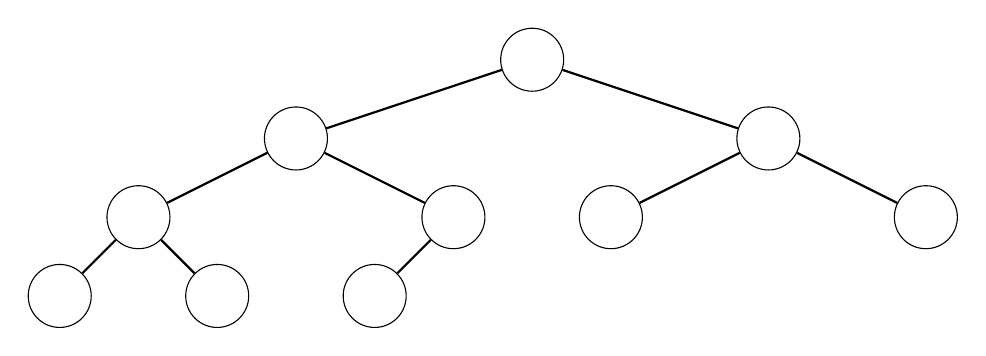
\begin{tikzpicture}
\node at (6,-1) [circle,draw,minimum size=8mm] (A) {};
\node at (3,-2) [circle,draw,minimum size=8mm] (B) {};
\node at (9,-2) [circle,draw,minimum size=8mm] (C) {};
\node at (1,-3) [circle,draw,minimum size=8mm] (D) {};
\node at (5,-3) [circle,draw,minimum size=8mm] (E) {};
\node at (7,-3) [circle,draw,minimum size=8mm] (F) {};
\node at (11,-3) [circle,draw,minimum size=8mm] (G) {};
\node at (0,-4) [circle,draw,minimum size=8mm] (H) {};
\node at (2,-4) [circle,draw,minimum size=8mm] (I) {};
\node at (4,-4) [circle,draw,minimum size=8mm] (J) {};
\draw [-,thick] (A) -- (B);
\draw [-,thick] (A) -- (C);
\draw [-,thick] (B) -- (D);
\draw [-,thick] (B) -- (E);
\draw [-,thick] (C) -- (G);
\draw [-,thick] (C) -- (F);
\draw [-,thick] (D) -- (H);
\draw [-,thick] (D) -- (I);
\draw [-,thick] (E) -- (J);

;
\end{tikzpicture}
    
\end{center}


\begin{console}
q->parent_->right_ = q->left_ // point 5 to 6
q->parent_ = p->parent_       // move 8 up to 10 
q->left_ = p->left_
q->right_ = p->right_
delete p
\end{console}

What is the runtime?
Again just like the BST search,
to reach the predessor or successor of the node you are trying to
delete, in the worst case, you have
travel along a path to a leaf.
So again the worst runtime is
\[
O(n)
\]
and again in the average case it's
\[
O(\log n)
\]
since all the above depends on the height of the BST tree.

\begin{console}
ALGORITHM: BST-DELETE
INPUT: node

if node has a left child:
    perform the operation to move the precedessor
    of the node up to the node's position
    and deallocate the appropriate node
else if node has a right child:
    perform the operation to move the sucessor
    of the node to the node's position
    and deallocate the appropriate node
else: // leaf case
    perform bst leaf delete on the node
\end{console}

Don't forget to correct the pseudocode using the exercises and warnings
given.
For instance look at the leaf case: what if the node
does not have a parent -- i.e., the node is in fact the root.


\begin{ex}
Now what if at the node to be deleted, there's exactly one child?
Can you use this information to get a better delete
operation?
For instance notice that in this bst, the node with 0 has a left
child but no right child:
\begin{center}
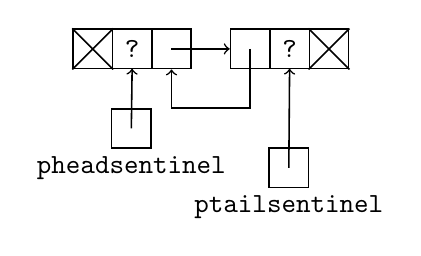
\begin{tikzpicture}

\draw (0.25, 0.25)
  node[draw, line width=0.02cm, , color=black,
       rounded corners=0cm, inner sep=0cm] {

\begin{minipage}[t][0.5cm]{0.5cm}
\mbox{}

\end{minipage}

};\draw (0.25, 0.25) node[color=black] {{\texttt{}}};
\draw (0.75, 0.25)
  node[draw, line width=0.02cm, , color=black,
       rounded corners=0cm, inner sep=0cm] {

\begin{minipage}[t][0.5cm]{0.5cm}
\mbox{}

\end{minipage}

};\draw (0.75, 0.25) node[color=black] {{\texttt{?}}};
\draw (1.25, 0.25)
  node[draw, line width=0.02cm, , color=black,
       rounded corners=0cm, inner sep=0cm] {

\begin{minipage}[t][0.5cm]{0.5cm}
\mbox{}

\end{minipage}

};\draw (1.25, 0.25) node[color=black] {{\texttt{}}};
\draw (2.25, 0.25)
  node[draw, line width=0.02cm, , color=black,
       rounded corners=0cm, inner sep=0cm] {

\begin{minipage}[t][0.5cm]{0.5cm}
\mbox{}

\end{minipage}

};\draw (2.25, 0.25) node[color=black] {{\texttt{}}};
\draw (2.75, 0.25)
  node[draw, line width=0.02cm, , color=black,
       rounded corners=0cm, inner sep=0cm] {

\begin{minipage}[t][0.5cm]{0.5cm}
\mbox{}

\end{minipage}

};\draw (2.75, 0.25) node[color=black] {{\texttt{?}}};
\draw (3.25, 0.25)
  node[draw, line width=0.02cm, , color=black,
       rounded corners=0cm, inner sep=0cm] {

\begin{minipage}[t][0.5cm]{0.5cm}
\mbox{}

\end{minipage}

};\draw (3.25, 0.25) node[color=black] {{\texttt{}}};\draw[line width=0.02cm,black,->] (1.25,0.25) to  (1.99,0.25);
\draw[line width=0.02cm,black,->] (2.25,0.25) to  (2.25,-0.5) to  (1.25,-0.5) to  (1.25,-0.01);
\draw[line width=0.02cm,black] (-0.01,0.51) to  (0.51,-0.01);
\draw[line width=0.02cm,black] (0.51,0.51) to  (-0.01,-0.01);
\draw[line width=0.02cm,black] (2.99,0.51) to  (3.51,-0.01);
\draw[line width=0.02cm,black] (3.51,0.51) to  (2.99,-0.01);

\draw (0.74, -0.76)
  node[draw, line width=0.02cm, , color=black,
       rounded corners=0cm, inner sep=0cm] {

\begin{minipage}[t][0.5cm]{0.5cm}
\mbox{}

\end{minipage}

};\draw (0.74, -0.76) node[color=black] {{\texttt{}}};
\draw (0.74, -1.26)
  node[draw, line width=0.02cm, , color=white,
       rounded corners=0cm, inner sep=0cm] {

\begin{minipage}[t][0.1cm]{0.1cm}
\mbox{}

\end{minipage}

};\draw (0.74, -1.26) node[color=black] {{\texttt{pheadsentinel}}};\draw[line width=0.02cm,black,->] (0.74,-0.76) to  (0.75,0);

\draw (2.74, -1.26)
  node[draw, line width=0.02cm, , color=black,
       rounded corners=0cm, inner sep=0cm] {

\begin{minipage}[t][0.5cm]{0.5cm}
\mbox{}

\end{minipage}

};\draw (2.74, -1.26) node[color=black] {{\texttt{}}};
\draw (2.74, -1.76)
  node[draw, line width=0.02cm, , color=white,
       rounded corners=0cm, inner sep=0cm] {

\begin{minipage}[t][0.1cm]{0.1cm}
\mbox{}

\end{minipage}

};\draw (2.74, -1.76) node[color=black] {{\texttt{ptailsentinel}}};\draw[line width=0.02cm,black,->] (2.74,-1.26) to  (2.75,0);
\end{tikzpicture}

\end{center}


If you perform the move-predecessor-up, then -1 replaces 0: draw the resulting
picture.
Can you draw another bst diagram that requires fewer changes to the original
bst?
Once you have this algorithm, modify the bst delete algorithm so that
it has this form:
\begin{console}
ALGORITHM: BST-DELETE
INPUT: node

if node has a left child but no right child:
    ...
else if node has a right child but no left child:
    ...
else if node has a right child and a left child:
    ...
else:
    ...
  \end{console}
\end{ex}


\begin{ex}
  \begin{tightlist}
    \li For the case where the node to be deleted has a left and a right child,
    write an algorithm that chooses the predecessor or successor based
    on the greedy approach: choose one that has the shortest depth from the
    node to be deleted.
    \li Is there any reason to choose the longest instead?
    \li Which of the above two is faster?
    \li What about flipping a coin? Why would you want to do that?
    \li How would you modify your BST to include information
    to better decide 
    on whether to move predecessor or sucessor up (instead of just
    tossing a coin)?
  \end{tightlist}
\end{ex}
% Last one: keep left-height and right-height in node. To save a bit more
% just save left-height minus right-height. Note that the update of
% height information is a little more costlier than size. So as an
% approximation, maybe keep leftsize and rightsize. Furthermore storing
% leftsize - rightsize is cheaper too.

\newpage
BST-DELETE algorithm:

Frequently it's convenient to have access to the parent's child point
that points to \verb!p!.
For instance if \verb!*p! is the right child or the parent
\verb!*(p->parent_)!, then it's convenient to have a function
to return a reference to \verb!p->parent_->right_!.
This can be used for any binary tree (not just bst).
This can be easily generalize to any tree.
\begin{console}
ALGORITHM: PARENT-CHILD-POINTER
INPUT:  p
RETURN: reference to left_ or right_ of *(p->parent)

let parent = p->parent_
if parent == NULL:
    return NULL // *p is root
else:
    if parent->left_ is p:
        return parent->left_ (by reference)
    else:
        return parent->right_
\end{console}

The following deletes the node \verb!*p! assuming that it's a leaf.
This can be easily generalized for any tree.
\begin{console}
ALGORITHM: LEAF-DELETE
INPUT: proot
       p

if *p is root:
    proot = NULL
else:
    PARENT-CHILD-POINTER(p) = NULL
delete p
\end{console}
(This is a general algorithm for binary trees, not just BST.)

The following cuts out a node $n$
directly from the tree so that the parent of $n$ is joined to
either the left or right child of $n$.
For instance if you perform punch through at 0 in the left direction.
It is also assumed that \verb!p! is not NULL and
\verb!p->parent_! is not NULL.
\begin{center}
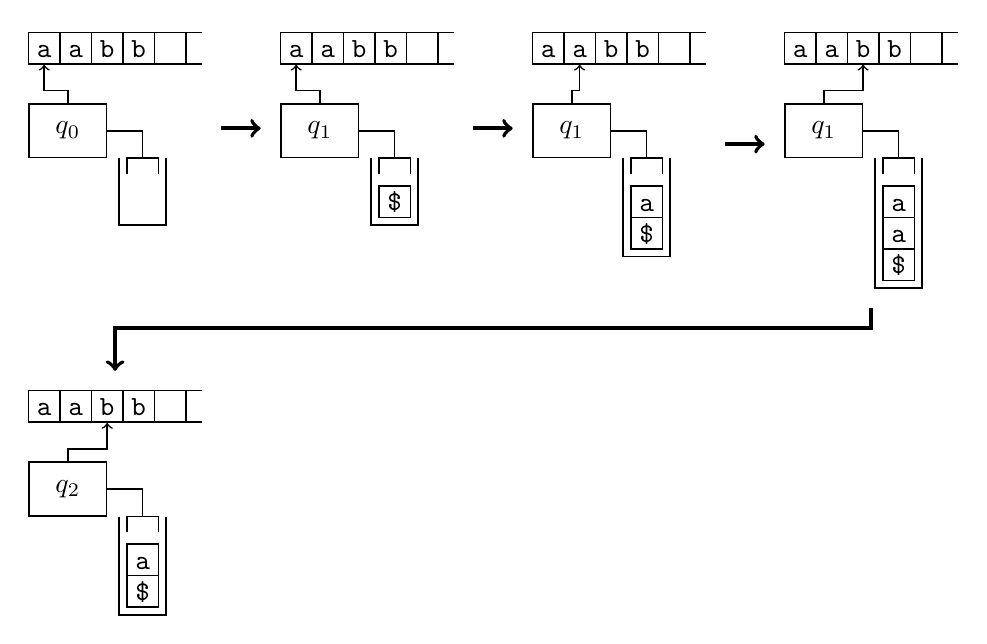
\begin{tikzpicture}

\draw (0.2, 0.2)
  node[draw, line width=0.02cm, , color=black,
       rounded corners=0cm, inner sep=0cm] {

\begin{minipage}[t][0.4cm]{0.4cm}
\mbox{}

\end{minipage}

};\draw (0.2, 0.2) node[color=black] {{\vphantom{aabb\SPACE}\texttt{a}}};
\draw (0.6000000000000001, 0.2)
  node[draw, line width=0.02cm, , color=black,
       rounded corners=0cm, inner sep=0cm] {

\begin{minipage}[t][0.4cm]{0.4cm}
\mbox{}

\end{minipage}

};\draw (0.6000000000000001, 0.2) node[color=black] {{\vphantom{aabb\SPACE}\texttt{a}}};
\draw (1.0, 0.2)
  node[draw, line width=0.02cm, , color=black,
       rounded corners=0cm, inner sep=0cm] {

\begin{minipage}[t][0.4cm]{0.4cm}
\mbox{}

\end{minipage}

};\draw (1.0, 0.2) node[color=black] {{\vphantom{aabb\SPACE}\texttt{b}}};
\draw (1.4000000000000001, 0.2)
  node[draw, line width=0.02cm, , color=black,
       rounded corners=0cm, inner sep=0cm] {

\begin{minipage}[t][0.4cm]{0.4cm}
\mbox{}

\end{minipage}

};\draw (1.4000000000000001, 0.2) node[color=black] {{\vphantom{aabb\SPACE}\texttt{b}}};
\draw (1.7999999999999998, 0.2)
  node[draw, line width=0.02cm, , color=black,
       rounded corners=0cm, inner sep=0cm] {

\begin{minipage}[t][0.4cm]{0.4cm}
\mbox{}

\end{minipage}

};\draw (1.7999999999999998, 0.2) node[color=black] {{\vphantom{aabb\SPACE}\texttt{\SPACE}}};\draw[line width=0.02cm,black] (2.0,0.4) to  (2.2,0.4);
\draw[line width=0.02cm,black] (2.0,0.0) to  (2.2,0.0);

\draw (0.5, -0.85)
  node[draw, line width=0.02cm, , color=black,
       rounded corners=0cm, inner sep=0cm] {

\begin{minipage}[t][0.68cm]{0.98cm}
\mbox{}

\end{minipage}

};\draw (0.5, -0.85) node[color=black] {$q_0$};\draw[line width=0.02cm,black,->] (0.5,-0.5) to  (0.5,-0.34) to  (0.2,-0.34) to  (0.2,-0.01);

\draw (1.45, -1.7499999999999998)
  node[draw=none, line width=0cm, , color=black,
       rounded corners=0cm, inner sep=0cm] {

\begin{minipage}[t][0.4cm]{0.4cm}
\mbox{}

\end{minipage}

};\draw[line width=0.02cm,black] (1.15,-1.2) to  (1.15,-2.05) to  (1.75,-2.05) to  (1.75,-1.2);
\draw[line width=0.02cm,black] (1,-0.85) to  (1.45,-0.85) to  (1.45,-1.2);
\draw[line width=0.02cm,black] (1.25,-1.4) to  (1.25,-1.2) to  (1.65,-1.2) to  (1.65,-1.4);
\draw[line width=0.05cm,black,->] (2.45,-0.82) to  (2.95,-0.82);

\draw (3.4000000000000004, 0.2)
  node[draw, line width=0.02cm, , color=black,
       rounded corners=0cm, inner sep=0cm] {

\begin{minipage}[t][0.4cm]{0.4cm}
\mbox{}

\end{minipage}

};\draw (3.4000000000000004, 0.2) node[color=black] {{\vphantom{\$aabb\SPACE}\texttt{a}}};
\draw (3.8, 0.2)
  node[draw, line width=0.02cm, , color=black,
       rounded corners=0cm, inner sep=0cm] {

\begin{minipage}[t][0.4cm]{0.4cm}
\mbox{}

\end{minipage}

};\draw (3.8, 0.2) node[color=black] {{\vphantom{\$aabb\SPACE}\texttt{a}}};
\draw (4.2, 0.2)
  node[draw, line width=0.02cm, , color=black,
       rounded corners=0cm, inner sep=0cm] {

\begin{minipage}[t][0.4cm]{0.4cm}
\mbox{}

\end{minipage}

};\draw (4.2, 0.2) node[color=black] {{\vphantom{\$aabb\SPACE}\texttt{b}}};
\draw (4.6000000000000005, 0.2)
  node[draw, line width=0.02cm, , color=black,
       rounded corners=0cm, inner sep=0cm] {

\begin{minipage}[t][0.4cm]{0.4cm}
\mbox{}

\end{minipage}

};\draw (4.6000000000000005, 0.2) node[color=black] {{\vphantom{\$aabb\SPACE}\texttt{b}}};
\draw (5.000000000000001, 0.2)
  node[draw, line width=0.02cm, , color=black,
       rounded corners=0cm, inner sep=0cm] {

\begin{minipage}[t][0.4cm]{0.4cm}
\mbox{}

\end{minipage}

};\draw (5.000000000000001, 0.2) node[color=black] {{\vphantom{\$aabb\SPACE}\texttt{\SPACE}}};\draw[line width=0.02cm,black] (5.200000000000001,0.4) to  (5.4,0.4);
\draw[line width=0.02cm,black] (5.200000000000001,0.0) to  (5.4,0.0);

\draw (3.7, -0.85)
  node[draw, line width=0.02cm, , color=black,
       rounded corners=0cm, inner sep=0cm] {

\begin{minipage}[t][0.68cm]{0.98cm}
\mbox{}

\end{minipage}

};\draw (3.7, -0.85) node[color=black] {$q_1$};\draw[line width=0.02cm,black,->] (3.7,-0.5) to  (3.7,-0.34) to  (3.4,-0.34) to  (3.4,-0.01);

\draw (4.65, -1.7499999999999998)
  node[draw, line width=0.02cm, , color=black,
       rounded corners=0cm, inner sep=0cm] {

\begin{minipage}[t][0.4cm]{0.4cm}
\mbox{}

\end{minipage}

};\draw (4.65, -1.7499999999999998) node[color=black] {{\vphantom{\$aabb\SPACE}\texttt{\$}}};\draw[line width=0.02cm,black] (4.35,-1.2) to  (4.35,-2.05) to  (4.95,-2.05) to  (4.95,-1.2);
\draw[line width=0.02cm,black] (4.2,-0.85) to  (4.65,-0.85) to  (4.65,-1.2);
\draw[line width=0.02cm,black] (4.45,-1.4) to  (4.45,-1.2) to  (4.85,-1.2) to  (4.85,-1.4);
\draw[line width=0.05cm,black,->] (5.65,-0.82) to  (6.15,-0.82);

\draw (6.600000000000001, 0.2)
  node[draw, line width=0.02cm, , color=black,
       rounded corners=0cm, inner sep=0cm] {

\begin{minipage}[t][0.4cm]{0.4cm}
\mbox{}

\end{minipage}

};\draw (6.600000000000001, 0.2) node[color=black] {{\vphantom{a\$aabb\SPACE}\texttt{a}}};
\draw (7.000000000000002, 0.2)
  node[draw, line width=0.02cm, , color=black,
       rounded corners=0cm, inner sep=0cm] {

\begin{minipage}[t][0.4cm]{0.4cm}
\mbox{}

\end{minipage}

};\draw (7.000000000000002, 0.2) node[color=black] {{\vphantom{a\$aabb\SPACE}\texttt{a}}};
\draw (7.400000000000002, 0.2)
  node[draw, line width=0.02cm, , color=black,
       rounded corners=0cm, inner sep=0cm] {

\begin{minipage}[t][0.4cm]{0.4cm}
\mbox{}

\end{minipage}

};\draw (7.400000000000002, 0.2) node[color=black] {{\vphantom{a\$aabb\SPACE}\texttt{b}}};
\draw (7.8000000000000025, 0.2)
  node[draw, line width=0.02cm, , color=black,
       rounded corners=0cm, inner sep=0cm] {

\begin{minipage}[t][0.4cm]{0.4cm}
\mbox{}

\end{minipage}

};\draw (7.8000000000000025, 0.2) node[color=black] {{\vphantom{a\$aabb\SPACE}\texttt{b}}};
\draw (8.200000000000003, 0.2)
  node[draw, line width=0.02cm, , color=black,
       rounded corners=0cm, inner sep=0cm] {

\begin{minipage}[t][0.4cm]{0.4cm}
\mbox{}

\end{minipage}

};\draw (8.200000000000003, 0.2) node[color=black] {{\vphantom{a\$aabb\SPACE}\texttt{\SPACE}}};\draw[line width=0.02cm,black] (8.400000000000002,0.4) to  (8.600000000000001,0.4);
\draw[line width=0.02cm,black] (8.400000000000002,0.0) to  (8.600000000000001,0.0);

\draw (6.900000000000001, -0.85)
  node[draw, line width=0.02cm, , color=black,
       rounded corners=0cm, inner sep=0cm] {

\begin{minipage}[t][0.68cm]{0.98cm}
\mbox{}

\end{minipage}

};\draw (6.900000000000001, -0.85) node[color=black] {$q_1$};\draw[line width=0.02cm,black,->] (6.9,-0.5) to  (6.9,-0.34) to  (7.0,-0.34) to  (7.0,-0.01);

\draw (7.850000000000001, -1.7499999999999998)
  node[draw, line width=0.02cm, , color=black,
       rounded corners=0cm, inner sep=0cm] {

\begin{minipage}[t][0.4cm]{0.4cm}
\mbox{}

\end{minipage}

};\draw (7.850000000000001, -1.7499999999999998) node[color=black] {{\vphantom{a\$aabb\SPACE}\texttt{a}}};
\draw (7.850000000000001, -2.1499999999999995)
  node[draw, line width=0.02cm, , color=black,
       rounded corners=0cm, inner sep=0cm] {

\begin{minipage}[t][0.4cm]{0.4cm}
\mbox{}

\end{minipage}

};\draw (7.850000000000001, -2.1499999999999995) node[color=black] {{\vphantom{a\$aabb\SPACE}\texttt{\$}}};\draw[line width=0.02cm,black] (7.55,-1.2) to  (7.55,-2.45) to  (8.15,-2.45) to  (8.15,-1.2);
\draw[line width=0.02cm,black] (7.4,-0.85) to  (7.85,-0.85) to  (7.85,-1.2);
\draw[line width=0.02cm,black] (7.65,-1.4) to  (7.65,-1.2) to  (8.05,-1.2) to  (8.05,-1.4);
\draw[line width=0.05cm,black,->] (8.85,-1.02) to  (9.35,-1.02);

\draw (9.8, 0.2)
  node[draw, line width=0.02cm, , color=black,
       rounded corners=0cm, inner sep=0cm] {

\begin{minipage}[t][0.4cm]{0.4cm}
\mbox{}

\end{minipage}

};\draw (9.8, 0.2) node[color=black] {{\vphantom{aa\$aabb\SPACE}\texttt{a}}};
\draw (10.200000000000003, 0.2)
  node[draw, line width=0.02cm, , color=black,
       rounded corners=0cm, inner sep=0cm] {

\begin{minipage}[t][0.4cm]{0.4cm}
\mbox{}

\end{minipage}

};\draw (10.200000000000003, 0.2) node[color=black] {{\vphantom{aa\$aabb\SPACE}\texttt{a}}};
\draw (10.600000000000001, 0.2)
  node[draw, line width=0.02cm, , color=black,
       rounded corners=0cm, inner sep=0cm] {

\begin{minipage}[t][0.4cm]{0.4cm}
\mbox{}

\end{minipage}

};\draw (10.600000000000001, 0.2) node[color=black] {{\vphantom{aa\$aabb\SPACE}\texttt{b}}};
\draw (11.000000000000004, 0.2)
  node[draw, line width=0.02cm, , color=black,
       rounded corners=0cm, inner sep=0cm] {

\begin{minipage}[t][0.4cm]{0.4cm}
\mbox{}

\end{minipage}

};\draw (11.000000000000004, 0.2) node[color=black] {{\vphantom{aa\$aabb\SPACE}\texttt{b}}};
\draw (11.400000000000002, 0.2)
  node[draw, line width=0.02cm, , color=black,
       rounded corners=0cm, inner sep=0cm] {

\begin{minipage}[t][0.4cm]{0.4cm}
\mbox{}

\end{minipage}

};\draw (11.400000000000002, 0.2) node[color=black] {{\vphantom{aa\$aabb\SPACE}\texttt{\SPACE}}};\draw[line width=0.02cm,black] (11.600000000000003,0.4) to  (11.800000000000002,0.4);
\draw[line width=0.02cm,black] (11.600000000000003,0.0) to  (11.800000000000002,0.0);

\draw (10.100000000000001, -0.85)
  node[draw, line width=0.02cm, , color=black,
       rounded corners=0cm, inner sep=0cm] {

\begin{minipage}[t][0.68cm]{0.98cm}
\mbox{}

\end{minipage}

};\draw (10.100000000000001, -0.85) node[color=black] {$q_1$};\draw[line width=0.02cm,black,->] (10.1,-0.5) to  (10.1,-0.34) to  (10.6,-0.34) to  (10.6,-0.01);

\draw (11.05, -1.7499999999999998)
  node[draw, line width=0.02cm, , color=black,
       rounded corners=0cm, inner sep=0cm] {

\begin{minipage}[t][0.4cm]{0.4cm}
\mbox{}

\end{minipage}

};\draw (11.05, -1.7499999999999998) node[color=black] {{\vphantom{aa\$aabb\SPACE}\texttt{a}}};
\draw (11.05, -2.1499999999999995)
  node[draw, line width=0.02cm, , color=black,
       rounded corners=0cm, inner sep=0cm] {

\begin{minipage}[t][0.4cm]{0.4cm}
\mbox{}

\end{minipage}

};\draw (11.05, -2.1499999999999995) node[color=black] {{\vphantom{aa\$aabb\SPACE}\texttt{a}}};
\draw (11.05, -2.55)
  node[draw, line width=0.02cm, , color=black,
       rounded corners=0cm, inner sep=0cm] {

\begin{minipage}[t][0.4cm]{0.4cm}
\mbox{}

\end{minipage}

};\draw (11.05, -2.55) node[color=black] {{\vphantom{aa\$aabb\SPACE}\texttt{\$}}};\draw[line width=0.02cm,black] (10.75,-1.2) to  (10.75,-2.85) to  (11.35,-2.85) to  (11.35,-1.2);
\draw[line width=0.02cm,black] (10.6,-0.85) to  (11.05,-0.85) to  (11.05,-1.2);
\draw[line width=0.02cm,black] (10.85,-1.4) to  (10.85,-1.2) to  (11.25,-1.2) to  (11.25,-1.4);
\draw[line width=0.05cm,black,->] (10.7,-3.1) to  (10.7,-3.35) to  (1.1,-3.35) to  (1.1,-3.9);

\draw (0.2, -4.35)
  node[draw, line width=0.02cm, , color=black,
       rounded corners=0cm, inner sep=0cm] {

\begin{minipage}[t][0.4cm]{0.4cm}
\mbox{}

\end{minipage}

};\draw (0.2, -4.35) node[color=black] {{\vphantom{a\$aabb\SPACE}\texttt{a}}};
\draw (0.6000000000000001, -4.35)
  node[draw, line width=0.02cm, , color=black,
       rounded corners=0cm, inner sep=0cm] {

\begin{minipage}[t][0.4cm]{0.4cm}
\mbox{}

\end{minipage}

};\draw (0.6000000000000001, -4.35) node[color=black] {{\vphantom{a\$aabb\SPACE}\texttt{a}}};
\draw (1.0, -4.35)
  node[draw, line width=0.02cm, , color=black,
       rounded corners=0cm, inner sep=0cm] {

\begin{minipage}[t][0.4cm]{0.4cm}
\mbox{}

\end{minipage}

};\draw (1.0, -4.35) node[color=black] {{\vphantom{a\$aabb\SPACE}\texttt{b}}};
\draw (1.4000000000000001, -4.35)
  node[draw, line width=0.02cm, , color=black,
       rounded corners=0cm, inner sep=0cm] {

\begin{minipage}[t][0.4cm]{0.4cm}
\mbox{}

\end{minipage}

};\draw (1.4000000000000001, -4.35) node[color=black] {{\vphantom{a\$aabb\SPACE}\texttt{b}}};
\draw (1.7999999999999998, -4.35)
  node[draw, line width=0.02cm, , color=black,
       rounded corners=0cm, inner sep=0cm] {

\begin{minipage}[t][0.4cm]{0.4cm}
\mbox{}

\end{minipage}

};\draw (1.7999999999999998, -4.35) node[color=black] {{\vphantom{a\$aabb\SPACE}\texttt{\SPACE}}};\draw[line width=0.02cm,black] (2.0,-4.1499999999999995) to  (2.2,-4.1499999999999995);
\draw[line width=0.02cm,black] (2.0,-4.55) to  (2.2,-4.55);

\draw (0.5, -5.4)
  node[draw, line width=0.02cm, , color=black,
       rounded corners=0cm, inner sep=0cm] {

\begin{minipage}[t][0.68cm]{0.98cm}
\mbox{}

\end{minipage}

};\draw (0.5, -5.4) node[color=black] {$q_2$};\draw[line width=0.02cm,black,->] (0.5,-5.05) to  (0.5,-4.89) to  (1.0,-4.89) to  (1.0,-4.56);

\draw (1.45, -6.300000000000001)
  node[draw, line width=0.02cm, , color=black,
       rounded corners=0cm, inner sep=0cm] {

\begin{minipage}[t][0.4cm]{0.4cm}
\mbox{}

\end{minipage}

};\draw (1.45, -6.300000000000001) node[color=black] {{\vphantom{a\$aabb\SPACE}\texttt{a}}};
\draw (1.45, -6.700000000000001)
  node[draw, line width=0.02cm, , color=black,
       rounded corners=0cm, inner sep=0cm] {

\begin{minipage}[t][0.4cm]{0.4cm}
\mbox{}

\end{minipage}

};\draw (1.45, -6.700000000000001) node[color=black] {{\vphantom{a\$aabb\SPACE}\texttt{\$}}};\draw[line width=0.02cm,black] (1.15,-5.75) to  (1.15,-7.0) to  (1.75,-7.0) to  (1.75,-5.75);
\draw[line width=0.02cm,black] (1,-5.4) to  (1.45,-5.4) to  (1.45,-5.75);
\draw[line width=0.02cm,black] (1.25,-5.95) to  (1.25,-5.75) to  (1.65,-5.75) to  (1.65,-5.95);
\end{tikzpicture}

\end{center}


we get
\input{stdout49.tex}
The algorithm deallocates the node that is punched through
but does not deallocate subtrees. For instance in the above
it's assumed that 0 does not have any right subtree to deallocate.
It allows \verb!p->parent_! to be NULL. In that case
a child of \verb!*p! becomes the root.
For instance if we punch through at 20 in the left direction for
the following tree
\begin{center}
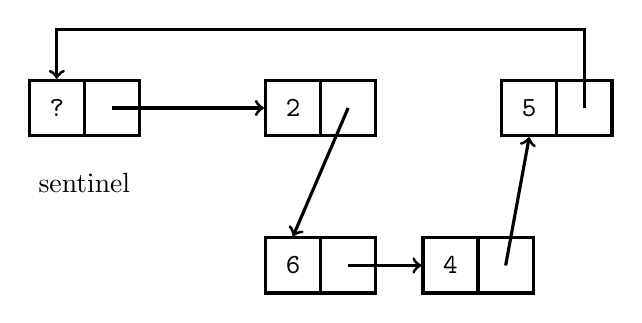
\begin{tikzpicture}

\draw (0.35, 0.35)
  node[draw, line width=0.04cm, , color=black,
       rounded corners=0cm, inner sep=0cm] {

\begin{minipage}[t][0.7cm]{0.7cm}
\mbox{}

\end{minipage}

};\draw (0.35, 0.35) node[color=black] {{\texttt{2}}};
\draw (1.0499999999999998, 0.35)
  node[draw, line width=0.04cm, , color=black,
       rounded corners=0cm, inner sep=0cm] {

\begin{minipage}[t][0.7cm]{0.7cm}
\mbox{}

\end{minipage}

};\draw (1.0499999999999998, 0.35) node[color=black] {{\texttt{}}};
\draw (0.35, -1.65)
  node[draw, line width=0.04cm, , color=black,
       rounded corners=0cm, inner sep=0cm] {

\begin{minipage}[t][0.7cm]{0.7cm}
\mbox{}

\end{minipage}

};\draw (0.35, -1.65) node[color=black] {{\texttt{6}}};
\draw (1.0499999999999998, -1.65)
  node[draw, line width=0.04cm, , color=black,
       rounded corners=0cm, inner sep=0cm] {

\begin{minipage}[t][0.7cm]{0.7cm}
\mbox{}

\end{minipage}

};\draw (1.0499999999999998, -1.65) node[color=black] {{\texttt{}}};
\draw (2.35, -1.65)
  node[draw, line width=0.04cm, , color=black,
       rounded corners=0cm, inner sep=0cm] {

\begin{minipage}[t][0.7cm]{0.7cm}
\mbox{}

\end{minipage}

};\draw (2.35, -1.65) node[color=black] {{\texttt{4}}};
\draw (3.0500000000000003, -1.65)
  node[draw, line width=0.04cm, , color=black,
       rounded corners=0cm, inner sep=0cm] {

\begin{minipage}[t][0.7cm]{0.7cm}
\mbox{}

\end{minipage}

};\draw (3.0500000000000003, -1.65) node[color=black] {{\texttt{}}};
\draw (3.35, 0.35)
  node[draw, line width=0.04cm, , color=black,
       rounded corners=0cm, inner sep=0cm] {

\begin{minipage}[t][0.7cm]{0.7cm}
\mbox{}

\end{minipage}

};\draw (3.35, 0.35) node[color=black] {{\texttt{5}}};
\draw (4.05, 0.35)
  node[draw, line width=0.04cm, , color=black,
       rounded corners=0cm, inner sep=0cm] {

\begin{minipage}[t][0.7cm]{0.7cm}
\mbox{}

\end{minipage}

};\draw (4.05, 0.35) node[color=black] {{\texttt{}}};
\draw (-2.65, 0.35)
  node[draw, line width=0.04cm, , color=black,
       rounded corners=0cm, inner sep=0cm] {

\begin{minipage}[t][0.7cm]{0.7cm}
\mbox{}

\end{minipage}

};\draw (-2.65, 0.35) node[color=black] {{\texttt{?}}};
\draw (-1.9499999999999997, 0.35)
  node[draw, line width=0.04cm, , color=black,
       rounded corners=0cm, inner sep=0cm] {

\begin{minipage}[t][0.7cm]{0.7cm}
\mbox{}

\end{minipage}

};\draw (-1.9499999999999997, 0.35) node[color=black] {{\texttt{}}};\draw[line width=0.04cm,black,->] (-1.95,0.35) to  (-0.02,0.35);
\draw[line width=0.04cm,black,->] (1.05,0.35) to  (0.35,-1.28);
\draw[line width=0.04cm,black,->] (1.05,-1.65) to  (1.98,-1.65);
\draw[line width=0.04cm,black,->] (3.05,-1.65) to  (3.35,-0.02);
\draw[line width=0.04cm,black,->] (4.05,0.35) to  (4.05,1.35) to  (-2.65,1.35) to  (-2.65,0.72);

\draw (-2.3, -0.6)
  node[draw=none, line width=0cm, , color=black,
       rounded corners=0cm, inner sep=0cm] {

\begin{minipage}[t][0.1cm]{0.1cm}
\mbox{}

\end{minipage}

};\draw (-2.3, -0.6) node[color=black] {sentinel};
\end{tikzpicture}

\end{center}


we get
\begin{center}
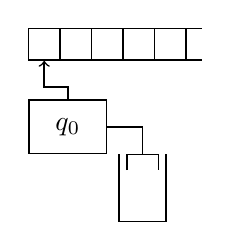
\begin{tikzpicture}

\draw (0.2, 0.2)
  node[draw, line width=0.02cm, , color=black,
       rounded corners=0cm, inner sep=0cm] {

\begin{minipage}[t][0.4cm]{0.4cm}
\mbox{}

\end{minipage}

};\draw (0.2, 0.2) node[color=black] {{\vphantom{\SPACE\SPACE\SPACE\SPACE\SPACE}\texttt{\SPACE}}};
\draw (0.6000000000000001, 0.2)
  node[draw, line width=0.02cm, , color=black,
       rounded corners=0cm, inner sep=0cm] {

\begin{minipage}[t][0.4cm]{0.4cm}
\mbox{}

\end{minipage}

};\draw (0.6000000000000001, 0.2) node[color=black] {{\vphantom{\SPACE\SPACE\SPACE\SPACE\SPACE}\texttt{\SPACE}}};
\draw (1.0, 0.2)
  node[draw, line width=0.02cm, , color=black,
       rounded corners=0cm, inner sep=0cm] {

\begin{minipage}[t][0.4cm]{0.4cm}
\mbox{}

\end{minipage}

};\draw (1.0, 0.2) node[color=black] {{\vphantom{\SPACE\SPACE\SPACE\SPACE\SPACE}\texttt{\SPACE}}};
\draw (1.4000000000000001, 0.2)
  node[draw, line width=0.02cm, , color=black,
       rounded corners=0cm, inner sep=0cm] {

\begin{minipage}[t][0.4cm]{0.4cm}
\mbox{}

\end{minipage}

};\draw (1.4000000000000001, 0.2) node[color=black] {{\vphantom{\SPACE\SPACE\SPACE\SPACE\SPACE}\texttt{\SPACE}}};
\draw (1.7999999999999998, 0.2)
  node[draw, line width=0.02cm, , color=black,
       rounded corners=0cm, inner sep=0cm] {

\begin{minipage}[t][0.4cm]{0.4cm}
\mbox{}

\end{minipage}

};\draw (1.7999999999999998, 0.2) node[color=black] {{\vphantom{\SPACE\SPACE\SPACE\SPACE\SPACE}\texttt{\SPACE}}};\draw[line width=0.02cm,black] (2.0,0.4) to  (2.2,0.4);
\draw[line width=0.02cm,black] (2.0,0.0) to  (2.2,0.0);

\draw (0.5, -0.85)
  node[draw, line width=0.02cm, , color=black,
       rounded corners=0cm, inner sep=0cm] {

\begin{minipage}[t][0.68cm]{0.98cm}
\mbox{}

\end{minipage}

};\draw (0.5, -0.85) node[color=black] {$q_0$};\draw[line width=0.02cm,black,->] (0.5,-0.5) to  (0.5,-0.34) to  (0.2,-0.34) to  (0.2,-0.01);

\draw (1.45, -1.7499999999999998)
  node[draw=none, line width=0cm, , color=black,
       rounded corners=0cm, inner sep=0cm] {

\begin{minipage}[t][0.4cm]{0.4cm}
\mbox{}

\end{minipage}

};\draw[line width=0.02cm,black] (1.15,-1.2) to  (1.15,-2.05) to  (1.75,-2.05) to  (1.75,-1.2);
\draw[line width=0.02cm,black] (1,-0.85) to  (1.45,-0.85) to  (1.45,-1.2);
\draw[line width=0.02cm,black] (1.25,-1.4) to  (1.25,-1.2) to  (1.65,-1.2) to  (1.65,-1.4);
\end{tikzpicture}

\end{center}



We can also punch through a node and go to the right.
For instance in the following,
\begin{center}
\begin{tikzpicture}

\fill[white] (11.0, 0.0) circle (0.3);
\node [line width=0.03cm,black,minimum size=0.57cm,draw,circle] at (11.0,0.0)(A){};\draw (11.0, 0.0) node[color=black] {\texttt{20}};
\fill[white] (10.0, -0.7) circle (0.3);
\node [line width=0.03cm,black,minimum size=0.57cm,draw,circle] at (10.0,-0.7)(a){};\draw (10.0, -0.7) node[color=black] {\texttt{10}};
\fill[white] (9.0, -1.4) circle (0.3);
\node [line width=0.03cm,black,minimum size=0.57cm,draw,circle] at (9.0,-1.4)(b){};\draw (9.0, -1.4) node[color=black] {\texttt{5}};
\fill[white] (10.0, -2.1) circle (0.3);
\node [line width=0.03cm,black,minimum size=0.57cm,draw,circle] at (10.0,-2.1)(e){};\draw (10.0, -2.1) node[color=black] {\texttt{8}};
\fill[white] (9.0, -2.8) circle (0.3);
\node [line width=0.03cm,black,minimum size=0.57cm,draw,circle] at (9.0,-2.8)(k){};\draw (9.0, -2.8) node[color=black] {\texttt{6}};
\fill[white] (11.0, -2.8) circle (0.3);
\node [line width=0.03cm,black,minimum size=0.57cm,draw,circle] at (11.0,-2.8)(l){};\draw (11.0, -2.8) node[color=black] {\texttt{9}};
\fill[white] (11.0, -1.4) circle (0.3);
\node [line width=0.03cm,black,minimum size=0.57cm,draw,circle] at (11.0,-1.4)(p){};\draw (11.0, -1.4) node[color=black] {\texttt{15}};\draw[line width=0.03cm,black,->,>=triangle 60] (A) to  (a);
\draw[line width=0.03cm,black,->,>=triangle 60] (a) to  (p);
\draw[line width=0.03cm,black,->,>=triangle 60] (a) to  (b);
\draw[line width=0.03cm,black,->,>=triangle 60] (b) to  (e);
\draw[line width=0.03cm,black,->,>=triangle 60] (e) to  (k);
\draw[line width=0.03cm,black,->,>=triangle 60] (e) to  (l);
\end{tikzpicture}

\end{center}


we can remove 5 by punching
through at 5 and go to the right to get this:
\input{stdout53.tex}
Here are the two algorithms for punch-through delete:
\begin{console}
ALGORITHM: PUNCH-THROUGH-TO-LEFT
INPUT: proot
       p

if p->parent is NULL:
    proot = p->left_
else:
    p->parent->left_ = p->left_
delete p
\end{console}
\begin{console}
ALGORITHM: PUNCH-THROUGH-TO-RIGHT
INPUT: proot
       p

if p->parent is NULL:
    proot = r->right_
else:
    p->parent->right_ = p->right_
delete p
\end{console}

This is the version without the punch-through deletion:
{\small
\begin{console}
ALGORITHM: BST-DELETE
INPUT: proot
       p

if p->left_ is NULL:
    if p->right_ is NULL:
        BST-DELETE-LEAF(proot, p)
    else:
        BST-MOVE-SUCC-UP(proot, p)
else:
    if p->right_ is NULL:
        BST-MOVE-PRED-UP(proot, p)
    else:
        # two children case
        if rand() % 2 == 0:
            BST-MOVE-PRED-UP(proot, p)
        else:
            BST-MOVE-SUCC-UP(proot, p)
\end{console}
}
This one uses the punch-through:
{\small
\begin{console}
ALGORITHM: BST-DELETE
INPUT: proot
       p

if p->left_ is NULL:
    if p->right_ is NULL:
        BST-DELETE-LEAF(proot, p)
    else:
        PUNCH-THROUGH-TO-RIGHT(proot, p)
else:
    if p_->right_ is NULL:
        PUNCH-THROUGH-TO-LEFT(proot, p)
    else:
        # two children case
        if rand() % 2 is 0:
            BST-MOVE-PRED-UP(proot, p)
        else:
            BST-MOVE-SUCC-UP(proot, p)
\end{console}
}

% To generalize, need to have some way of telling the path to the root
% for instance p should contain the pointers of ancestors back to root
% a recursive function contains only aancestor chain of nodes but not the
% point use to move down
% maybe nodes should contain reference/pointer to the parent's pointer
% leading to the node
% Call this the parent_child_ptr the pointer in *(p->parent) that points
% to p
% To delete *p from parent do
%     *(p->parent_child_ptr_) = NULL
%     delete p
% If this is not kept in the node, then can also keep inside an iterator
% Maybe an iterator should contain
% - pointer to node
% - pointer to parent (in case node does not have parent pointer)
% - pointer to pointer in parent that points to node
% For recusive functions, maybe should write them like this:
%
% void f(p):
%     if p == null:
%         return
%     else:
%         Node ** child_pointer
%         if ...
%             child_pointer = &(p->left_)
%             f(p->left_)
%         else:
%             child_pointer = &(p->right_)
%             f(p->right_)
%
%         do some more computation on *p possibly using
%         parent_child_pointer



\newpage
\begin{ex}
  Write a function
\begin{console}
bool is_bst(Node * p);
\end{console}
that checks if the binary tree at \verb!p! is a BST.
\end{ex}



\newpage
\begin{ex}
  Suppose you're given an array of integers which is already
  sorted in ascending order.
  How would your construct a BST with the values in this array
  so that the height of the tree is as small as possible?
\end{ex}
% build(arr, start=0, end=n-1, p)
%    if start >= end:
%        return NULL
%    else
%        mid = (start + end) / 2
%        leftroot = build(arr, start, m-id - 1)
%        rightroot = build(arr, mid + 1, end)
%        p = new Node(mid)   
%        p->left_ = leftroot
%        p->right_ = rightroot
% -- note that this is postorder except that the tree does not
%    exist yet. So technically not a traversal



\newpage
\begin{ex}
  Range search:
  Let $a < b$ and $T$ be a BST.
  \begin{itemize}
    \li Write a function that returns true if there is a key
    $k$ such that $a \leq k < b$.
    \li Write a function that returns a pointer
    that points to the node in $T$
    with the smallest key $k$ such that
    $a \leq k < b$.
    If there is none, NULL is returned.
    \li Write a function that accepts a pointer $p$,
    and a value $b$ and that returns a pointer
    that points to the node in $T$
    with the smallest key $k$ such that
    \verb!p->key_! $< k < b$.
    If there is none, NULL is returned.
    
    \li Write a function that returns a vector or list of pointers
    pointing to all nodes in $T$ with values in $[a, b)$.
    The pointers must be arranged in order of the key values of their
    nodes.

    \li Write an iterator class so that that does the same as
    the above. For instance \verb!BST_iterator p(proot, a, b)!
    will create the iterator and you iterate through all the
    pointers of the required nodes by doing
    {\small
    \begin{Verbatim}[frame=single]
while (p != NULL)
{
    std::cout << p->key() << '\n';
    ++p;
}
    \end{Verbatim}
    }
  \end{itemize}
\end{ex}

  
\newpage
\subsection{Comparing BST and sorted array}

I hope that you see that the BST search if the tree is balanced (i.e.,
roughyl equal number of nodes on the left and right for each node),
the nodes that you visit is similar to the values you would
visit in a sorted array with the same values.

Here's our first BST again:

\input{stdout54.tex}

Suppose I make the tree completedly balanced:
\begin{center}
\begin{tikzpicture}

\fill[white] (20.0, -2.0) circle (0.3);
\node [line width=0.03cm,black,minimum size=0.57cm,draw,circle] at (20.0,-2.0)(A){};\draw (20.0, -2.0) node[color=black] {\texttt{20}};
\fill[white] (14.0, 0.0) circle (0.3);
\node [line width=0.03cm,black,minimum size=0.57cm,draw,circle] at (14.0,0.0)(a){};\draw (14.0, 0.0) node[color=black] {\texttt{10}};
\fill[white] (10.0, -1.0) circle (0.3);
\node [line width=0.03cm,black,minimum size=0.57cm,draw,circle] at (10.0,-1.0)(b){};\draw (10.0, -1.0) node[color=black] {\texttt{4}};
\fill[white] (18.0, -1.0) circle (0.3);
\node [line width=0.03cm,black,minimum size=0.57cm,draw,circle] at (18.0,-1.0)(p){};\draw (18.0, -1.0) node[color=black] {\texttt{18}};
\fill[white] (8.0, -2.0) circle (0.3);
\node [line width=0.03cm,black,minimum size=0.57cm,draw,circle] at (8.0,-2.0)(e){};\draw (8.0, -2.0) node[color=black] {\texttt{2}};
\fill[white] (7.0, -3.0) circle (0.3);
\node [line width=0.03cm,black,minimum size=0.57cm,draw,circle] at (7.0,-3.0)(k){};\draw (7.0, -3.0) node[color=black] {\texttt{0}};
\fill[white] (9.0, -3.0) circle (0.3);
\node [line width=0.03cm,black,minimum size=0.57cm,draw,circle] at (9.0,-3.0)(l){};\draw (9.0, -3.0) node[color=black] {\texttt{3}};
\fill[white] (16.0, -2.0) circle (0.3);
\node [line width=0.03cm,black,minimum size=0.57cm,draw,circle] at (16.0,-2.0)(h){};\draw (16.0, -2.0) node[color=black] {\texttt{15}};
\fill[white] (15.0, -3.0) circle (0.3);
\node [line width=0.03cm,black,minimum size=0.57cm,draw,circle] at (15.0,-3.0)(m){};\draw (15.0, -3.0) node[color=black] {\texttt{12}};
\fill[white] (12.0, -2.0) circle (0.3);
\node [line width=0.03cm,black,minimum size=0.57cm,draw,circle] at (12.0,-2.0)(f){};\draw (12.0, -2.0) node[color=black] {\texttt{8}};
\fill[white] (11.0, -3.0) circle (0.3);
\node [line width=0.03cm,black,minimum size=0.57cm,draw,circle] at (11.0,-3.0)(n){};\draw (11.0, -3.0) node[color=black] {\texttt{6}};
\fill[white] (13.0, -3.0) circle (0.3);
\node [line width=0.03cm,black,minimum size=0.57cm,draw,circle] at (13.0,-3.0)(o){};\draw (13.0, -3.0) node[color=black] {\texttt{9}};
\fill[white] (17.0, -3.0) circle (0.3);
\node [line width=0.03cm,black,minimum size=0.57cm,draw,circle] at (17.0,-3.0)(q){};\draw (17.0, -3.0) node[color=black] {\texttt{17}};
\fill[white] (19.0, -3.0) circle (0.3);
\node [line width=0.03cm,black,minimum size=0.57cm,draw,circle] at (19.0,-3.0)(r){};\draw (19.0, -3.0) node[color=black] {\texttt{19}};
\fill[white] (21.0, -3.0) circle (0.3);
\node [line width=0.03cm,black,minimum size=0.57cm,draw,circle] at (21.0,-3.0)(s){};\draw (21.0, -3.0) node[color=black] {\texttt{22}};\draw[line width=0.03cm,black,->,>=triangle 60] (a) to  (p);
\draw[line width=0.03cm,black,->,>=triangle 60] (h) to  (m);
\draw[line width=0.03cm,black,->,>=triangle 60] (a) to  (b);
\draw[line width=0.03cm,black,->,>=triangle 60] (p) to  (h);
\draw[line width=0.03cm,black,->,>=triangle 60] (p) to  (A);
\draw[line width=0.03cm,black,->,>=triangle 60] (A) to  (r);
\draw[line width=0.03cm,black,->,>=triangle 60] (A) to  (s);
\draw[line width=0.03cm,black,->,>=triangle 60] (b) to  (e);
\draw[line width=0.03cm,black,->,>=triangle 60] (b) to  (f);
\draw[line width=0.03cm,black,->,>=triangle 60] (e) to  (k);
\draw[line width=0.03cm,black,->,>=triangle 60] (e) to  (l);
\draw[line width=0.03cm,black,->,>=triangle 60] (f) to  (o);
\draw[line width=0.03cm,black,->,>=triangle 60] (h) to  (q);
\draw[line width=0.03cm,black,->,>=triangle 60] (f) to  (n);
\end{tikzpicture}

\end{center}



Here's another way to store the data, i.e., as a sorted array:
\begin{center}
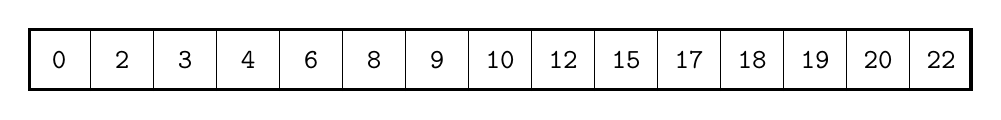
\begin{tikzpicture}

\draw (6.5, 0.9)
  node[draw, line width=0.04cm, , color=black,
       rounded corners=0.0cm, inner sep=0.0cm] {

\begin{minipage}[t][0.76cm]{11.96cm}
\mbox{}

\end{minipage}

};\draw[, font=\ttfamily] (0.9, 0.9) node {0};
\draw[black] (1.3,0.5) to  (1.3,1.3);
\draw[, font=\ttfamily] (1.7000000000000002, 0.9) node {2};
\draw[black] (2.1,0.5) to  (2.1,1.3);
\draw[, font=\ttfamily] (2.5, 0.9) node {3};
\draw[black] (2.9000000000000004,0.5) to  (2.9000000000000004,1.3);
\draw[, font=\ttfamily] (3.3, 0.9) node {4};
\draw[black] (3.7,0.5) to  (3.7,1.3);
\draw[, font=\ttfamily] (4.1, 0.9) node {6};
\draw[black] (4.5,0.5) to  (4.5,1.3);
\draw[, font=\ttfamily] (4.8999999999999995, 0.9) node {8};
\draw[black] (5.3,0.5) to  (5.3,1.3);
\draw[, font=\ttfamily] (5.699999999999999, 0.9) node {9};
\draw[black] (6.1,0.5) to  (6.1,1.3);
\draw[, font=\ttfamily] (6.499999999999999, 0.9) node {10};
\draw[black] (6.8999999999999995,0.5) to  (6.8999999999999995,1.3);
\draw[, font=\ttfamily] (7.299999999999999, 0.9) node {12};
\draw[black] (7.699999999999999,0.5) to  (7.699999999999999,1.3);
\draw[, font=\ttfamily] (8.1, 0.9) node {15};
\draw[black] (8.5,0.5) to  (8.5,1.3);
\draw[, font=\ttfamily] (8.9, 0.9) node {17};
\draw[black] (9.3,0.5) to  (9.3,1.3);
\draw[, font=\ttfamily] (9.700000000000001, 0.9) node {18};
\draw[black] (10.100000000000001,0.5) to  (10.100000000000001,1.3);
\draw[, font=\ttfamily] (10.500000000000002, 0.9) node {19};
\draw[black] (10.900000000000002,0.5) to  (10.900000000000002,1.3);
\draw[, font=\ttfamily] (11.300000000000002, 0.9) node {20};
\draw[black] (11.700000000000003,0.5) to  (11.700000000000003,1.3);
\draw[, font=\ttfamily] (12.100000000000003, 0.9) node {22};
\end{tikzpicture}

\end{center}



If you search for \texttt{6} in the BST above using BST search you will
visit the same values if you perform binary search on the sorted array for
\texttt{6}.


\newpage
\begin{ex}
Perform BST search on the above tree to look for \texttt{6}
and note down
the values you visit.
Now do binary search on the sorted array to look for \texttt{6}.
Maker sure you visit the same values in both cases.
Do the same for \texttt{0}.
\qed
\end{ex}


\newpage
Same runtime performance!

Remember ... the memory usage of array is not good if the array size
is big because you need a huge contiguous chunk of memory to satisfy
the memory allocation.
That's why we used nodes, forming a linked list.
\textit{But} ... the problem with the linked list is that
although memory usage is great, binary search is not possible.
Search for a value in a linked list is $O(n)$ in the worst case.
It's true that in the case of a BST search, \text{if}
the tree is roughly balanced (which is the average case),
the BST search has an average runtime of
\[
O(\log n)
\]

But that's not the end of the story:
Insert and delete for an array (sorted or not)
is in the average/worst case
\[
O(n)
\]
But if a BST tree is balanced (which is the average),
the insert and delete are both
\[
O(\log n)
\]
It does have a worst case of $O(n)$.

Everything is perfect and in the average case,
insert, delete, and search are all
\[
O(\log n)
\]
Meaning to say that average over all BST of size $n$,
the above runtimes hold.
\texttt{But} ... if you're always working with
\texttt{one} fixed BST that is heavily unbalanced,
then you're out of luck.
The question is then ... can we force a tree to be balanced?
 % done
\newpage%-*-latex-*-
\sectionthree{Rotations; Self-Balancing AVL BST}
\begin{python0}
from solutions import *; clear()
\end{python0}

\subsection{Left and right rotations}

As I said in previous sections, we want to use search trees to store data
and we want to search for a particular data very quickly.
The number of iterations that must be carried out is at
worse the height of the tree.
So we want the height to be as small as possible.
Which is the same as saying, for the case of a binary search tree,
the height of the left subtree
is roughly the same as the height of the right subtree.

The sense of being height balanced is a definition not just at the root
of the BST, but at every node.
Why?
Because if the tree is not height balanced, then there are two leaves
that will meet at a common ancentor $c$ and the lengths of their
path are significantly different.
The way to \lq\lq repair'' the the tree is to repair the subtree with
root $c$ first.
The operation is more or less to more some nodes from the taller
subtree of $c$ to the shorter subtree.
This is achieved through two operators:
the left rotation and right rotation about a node.

You can define left and right rotations about any node.
So first I'll describe the left and right rotations and then talk about
AVL trees, i.e., height balanced BST.

The following describes the left rotation operation about 
$\alpha$:

\begin{center}
\begin{tikzpicture}[>=triangle 60,shorten >=0.5pt,node distance=2cm,auto,initial text=, double distance=2pt]
\node[state,initial] (A) at (  0,  0) {$1$};
\node[state] (B) at (  3,  0) {$2$};
\node[state] (D) at (  0, -2) {$4$};
\node[state] (C) at (  3, -2) {$3$};

\path[->]
(A) edge [bend left=0,pos=0.5,above] node {$(\ep,\ep\rightarrow\$)$} (B)
(B) edge [loop above] node {$(a, \ep\rightarrow a)$} ()
(B) edge [bend left=0,pos=0.5] node {$(b,a\rightarrow\ep)$} (C)
(C) edge [bend left=0,pos=0.5] node {$(\ep,\ep\rightarrow \$)$} (D)

;
\end{tikzpicture}
\end{center}
    


\begin{center}
\begin{tikzpicture}[>=triangle 60,shorten >=0.5pt,node distance=2cm,auto,initial text=, double distance=2pt]
\node[state] (A) at (  0,  0) {$p$};
\node[state] (B) at (  3,  0) {$q$};

\path[->]
(A) edge [bend left=0,pos=0.5,above] node {$a, b\rightarrow c$} (B)

;
\end{tikzpicture}
\end{center}
    


\begin{center}
\begin{tikzpicture}[>=triangle 60,shorten >=0.5pt,node distance=2cm,auto,initial text=, double distance=2pt]
\node[state] (C) at (  0,  0) {$p$};
\node[state] (D) at (  5,  0) {new state};
\node[state] (E) at ( 10,  0) {$q$};

\path[->]
(C) edge [bend left=0,pos=0.5,above] node {$a,b\rightarrow\epsilon\text{ (pop)}$} (D)
(D) edge [bend left=0,pos=0.5,above] node {$\epsilon,\epsilon\rightarrow c\text{ (push)}$ } (E)

;
\end{tikzpicture}
\end{center}
    


Note that the trees $T_1, T_2$, and $T_3$ can be empty.
Also, note that to left rotate at $\alpha$, $\alpha$ must have a right child.


Right rotation is similar.
Here's the right rotation about $\alpha$:


\begin{center}
\begin{tikzpicture}[>=triangle 60,shorten >=0.5pt,node distance=2cm,auto,initial text=, double distance=2pt]
\node[state] (B) at (  3,  0) {$2$};
\node[state] (C) at (  5,  0) {$2$};
\node[state] (A) at (  0, -2) {$1$};
\node[state] (D) at (  8, -2) {$2$};

\path[->]
(A) edge [bend left=0,pos=0.5,above] node {$\ep,\ep\rightarrow\$$} (B)
(C) edge [bend left=0,pos=0.5,above] node {$a,\ep\rightarrow a$} (D)

;
\end{tikzpicture}
\end{center}
    

\input{stdout61.tex}

\begin{center}

\begin{tikzpicture}
\node at (4,-0.8) [minimum size=8mm] (Z) {$$};
\node at (2,-1.6) [circle,draw,minimum size=8mm] (A) {$\beta$};
\node at (0,-2.4000000000000004)
    [isosceles triangle, shape border rotate=+90,
     draw,minimum size=8mm,minimum height=2cm,
     anchor=north] (Ctriangle) {$T_1$};
\coordinate (C) at (0,-2.4000000000000004);
\node at (4,-2.4000000000000004) [circle,draw,minimum size=8mm] (B) {$\alpha$};
\node at (3,-3.2)
    [isosceles triangle, shape border rotate=+90,
     draw,minimum size=8mm,minimum height=2cm,
     anchor=north] (Dtriangle) {$T_2$};
\coordinate (D) at (3,-3.2);
\node at (5,-3.2)
    [isosceles triangle, shape border rotate=+90,
     draw,minimum size=8mm,minimum height=2cm,
     anchor=north] (Etriangle) {$T_3$};
\coordinate (E) at (5,-3.2);
\draw [-,thick] (Z) -- (A);
\draw [-,thick] (A) -- (B);
\draw [-,thick] (A) -- (C);
\draw [-,thick] (B) -- (D);
\draw [-,thick] (B) -- (E);

;
\end{tikzpicture}
    
\end{center}


Note that $\alpha$ must have a left child if you want to
right rotate at $\alpha$.

It's clear that the above
left and right rotations required constant time.

Here are some examples on left and right rotations.
At this point, don't worry about the balance of the tree yet.
We'll come to that after you understand the left and right rotations.

\begin{eg}
  Suppose I have this BST $T$:
  \input{stdout63.tex}
  
(a):
When I perform a left rotation on $T$ about node \verb!10! I get:
  \begin{center}
\begin{tikzpicture}

\fill[white] (5.0, 0.0) circle (0.3);
\node [draw=none,line width=0cm,black,minimum size=0.6cm,circle] at (5.0,0.0)(X){};
\fill[white] (17.0, 0.0) circle (0.3);
\node [draw=none,line width=0cm,black,minimum size=0.6cm,circle] at (17.0,0.0)(Y){};
\fill[white] (11.0, 0.0) circle (0.3);
\node [line width=0.03cm,black,minimum size=0.57cm,draw,circle] at (11.0,0.0)(a){};\draw (11.0, 0.0) node[color=black] {\texttt{18}};
\fill[white] (9.0, -1.0) circle (0.3);
\node [line width=0.03cm,black,minimum size=0.57cm,draw,circle] at (9.0,-1.0)(b){};\draw (9.0, -1.0) node[color=black] {\texttt{10}};
\fill[white] (14.0, -2.0) circle (0.3);
\node [line width=0.03cm,black,minimum size=0.57cm,draw,circle] at (14.0,-2.0)(d){};\draw (14.0, -2.0) node[color=black] {\texttt{20}};
\fill[white] (8.0, -2.0) circle (0.3);
\node [line width=0.03cm,black,minimum size=0.57cm,draw,circle] at (8.0,-2.0)(e){};\draw (8.0, -2.0) node[color=black] {\texttt{4}};
\fill[white] (12.0, -2.0) circle (0.3);
\node [line width=0.03cm,black,minimum size=0.57cm,draw,circle] at (12.0,-2.0)(f){};\draw (12.0, -2.0) node[color=black] {\texttt{19}};
\fill[white] (8.0, -4.0) circle (0.3);
\node [line width=0.03cm,black,minimum size=0.57cm,draw,circle] at (8.0,-4.0)(k){};\draw (8.0, -4.0) node[color=black] {\texttt{3}};
\fill[white] (7.0, -3.0) circle (0.3);
\node [line width=0.03cm,black,minimum size=0.57cm,draw,circle] at (7.0,-3.0)(l){};\draw (7.0, -3.0) node[color=black] {\texttt{2}};
\fill[white] (13.0, -1.0) circle (0.3);
\node [line width=0.03cm,black,minimum size=0.57cm,draw,circle] at (13.0,-1.0)(p){};\draw (13.0, -1.0) node[color=black] {\texttt{26}};
\fill[white] (6.0, -4.0) circle (0.3);
\node [line width=0.03cm,black,minimum size=0.57cm,draw,circle] at (6.0,-4.0)(n){};\draw (6.0, -4.0) node[color=black] {\texttt{0}};
\fill[white] (10.0, -2.0) circle (0.3);
\node [line width=0.03cm,black,minimum size=0.57cm,draw,circle] at (10.0,-2.0)(q){};\draw (10.0, -2.0) node[color=black] {\texttt{17}};\draw[line width=0.03cm,black,->,>=triangle 60] (e) to  (l);
\draw[line width=0.03cm,black,->,>=triangle 60] (p) to  (d);
\draw[line width=0.03cm,black,->,>=triangle 60] (b) to  (q);
\draw[line width=0.03cm,black,->,>=triangle 60] (l) to  (n);
\draw[line width=0.03cm,black,->,>=triangle 60] (l) to  (k);
\draw[line width=0.03cm,black,->,>=triangle 60] (p) to  (f);
\draw[line width=0.03cm,black,->,>=triangle 60] (a) to  (p);
\draw[line width=0.03cm,black,->,>=triangle 60] (a) to  (b);
\draw[line width=0.03cm,black,->,>=triangle 60] (b) to  (e);
\end{tikzpicture}

\end{center}



(b):
When I perform a right rotation on $T$ about node \verb!10! I get:
  \begin{center}
\begin{tikzpicture}

\fill[white] (5.0, 0.0) circle (0.3);
\node [draw=none,line width=0cm,black,minimum size=0.6cm,circle] at (5.0,0.0)(X){};
\fill[white] (17.0, 0.0) circle (0.3);
\node [draw=none,line width=0cm,black,minimum size=0.6cm,circle] at (17.0,0.0)(Y){};
\fill[white] (13.0, -1.0) circle (0.3);
\node [line width=0.03cm,black,minimum size=0.57cm,draw,circle] at (13.0,-1.0)(a){};\draw (13.0, -1.0) node[color=black] {\texttt{10}};
\fill[white] (11.0, 0.0) circle (0.3);
\node [line width=0.03cm,black,minimum size=0.57cm,draw,circle] at (11.0,0.0)(b){};\draw (11.0, 0.0) node[color=black] {\texttt{4}};
\fill[white] (15.0, -3.0) circle (0.3);
\node [line width=0.03cm,black,minimum size=0.57cm,draw,circle] at (15.0,-3.0)(d){};\draw (15.0, -3.0) node[color=black] {\texttt{20}};
\fill[white] (9.0, -1.0) circle (0.3);
\node [line width=0.03cm,black,minimum size=0.57cm,draw,circle] at (9.0,-1.0)(e){};\draw (9.0, -1.0) node[color=black] {\texttt{2}};
\fill[white] (13.0, -3.0) circle (0.3);
\node [line width=0.03cm,black,minimum size=0.57cm,draw,circle] at (13.0,-3.0)(f){};\draw (13.0, -3.0) node[color=black] {\texttt{17}};
\fill[white] (8.0, -2.0) circle (0.3);
\node [line width=0.03cm,black,minimum size=0.57cm,draw,circle] at (8.0,-2.0)(k){};\draw (8.0, -2.0) node[color=black] {\texttt{0}};
\fill[white] (10.0, -2.0) circle (0.3);
\node [line width=0.03cm,black,minimum size=0.57cm,draw,circle] at (10.0,-2.0)(l){};\draw (10.0, -2.0) node[color=black] {\texttt{3}};
\fill[white] (14.0, -2.0) circle (0.3);
\node [line width=0.03cm,black,minimum size=0.57cm,draw,circle] at (14.0,-2.0)(p){};\draw (14.0, -2.0) node[color=black] {\texttt{18}};
\fill[white] (14.0, -4.0) circle (0.3);
\node [line width=0.03cm,black,minimum size=0.57cm,draw,circle] at (14.0,-4.0)(h){};\draw (14.0, -4.0) node[color=black] {\texttt{19}};
\fill[white] (16.0, -4.0) circle (0.3);
\node [line width=0.03cm,black,minimum size=0.57cm,draw,circle] at (16.0,-4.0)(m){};\draw (16.0, -4.0) node[color=black] {\texttt{26}};\draw[line width=0.03cm,black,->,>=triangle 60] (b) to  (a);
\draw[line width=0.03cm,black,->,>=triangle 60] (p) to  (f);
\draw[line width=0.03cm,black,->,>=triangle 60] (p) to  (d);
\draw[line width=0.03cm,black,->,>=triangle 60] (a) to  (p);
\draw[line width=0.03cm,black,->,>=triangle 60] (b) to  (e);
\draw[line width=0.03cm,black,->,>=triangle 60] (e) to  (k);
\draw[line width=0.03cm,black,->,>=triangle 60] (e) to  (l);
\draw[line width=0.03cm,black,->,>=triangle 60] (d) to  (h);
\draw[line width=0.03cm,black,->,>=triangle 60] (d) to  (m);
\end{tikzpicture}

\end{center}



(c): I cannot perform a left rotation on $T$ about
node 4 because 4 does not have a right child.

(d):
When I perform a right rotation on $T$ about node \verb!4! I get:
\input{stdout66.tex}

(e): Perform a left rotation at 18.

(f): Perform a right rotation at 18.

(g): Perform a left rotation at 2.

(h): Perform a right rotation at 2.

(i): Why can't you perform a left rotation at 17?

(j): Why can't you perform a right rotation at 17?

(k): Perform a left rotation at 20.

(l): Perform a right rotation at 20.

\end{eg}

\newpage
\begin{ex}
  You are given the following BST $T$:
  \begin{center}
\begin{tikzpicture}

\fill[white] (0.0, 0.0) circle (0.3);
\node [line width=0.03cm,black,minimum size=0.57cm,draw,circle] at (0.0,0.0)(14){};\draw (0.0, 0.0) node[color=black] {\texttt{14}};
\fill[white] (-3.2, -1.0) circle (0.3);
\node [line width=0.03cm,black,minimum size=0.57cm,draw,circle] at (-3.2,-1.0)(9){};\draw (-3.2, -1.0) node[color=black] {\texttt{9}};
\fill[white] (3.2, -1.0) circle (0.3);
\node [line width=0.03cm,black,minimum size=0.57cm,draw,circle] at (3.2,-1.0)(18){};\draw (3.2, -1.0) node[color=black] {\texttt{18}};
\fill[white] (-4.8, -2.0) circle (0.3);
\node [line width=0.03cm,black,minimum size=0.57cm,draw,circle] at (-4.8,-2.0)(5){};\draw (-4.8, -2.0) node[color=black] {\texttt{5}};
\fill[white] (-1.6, -2.0) circle (0.3);
\node [line width=0.03cm,black,minimum size=0.57cm,draw,circle] at (-1.6,-2.0)(13){};\draw (-1.6, -2.0) node[color=black] {\texttt{13}};
\fill[white] (1.6, -2.0) circle (0.3);
\node [line width=0.03cm,black,minimum size=0.57cm,draw,circle] at (1.6,-2.0)(15){};\draw (1.6, -2.0) node[color=black] {\texttt{15}};
\fill[white] (4.8, -2.0) circle (0.3);
\node [line width=0.03cm,black,minimum size=0.57cm,draw,circle] at (4.8,-2.0)(22){};\draw (4.8, -2.0) node[color=black] {\texttt{22}};
\fill[white] (-5.6, -3.0) circle (0.3);
\node [line width=0.03cm,black,minimum size=0.57cm,draw,circle] at (-5.6,-3.0)(0){};\draw (-5.6, -3.0) node[color=black] {\texttt{0}};
\fill[white] (-4.0, -3.0) circle (0.3);
\node [line width=0.03cm,black,minimum size=0.57cm,draw,circle] at (-4.0,-3.0)(8){};\draw (-4.0, -3.0) node[color=black] {\texttt{8}};
\fill[white] (-2.4, -3.0) circle (0.3);
\node [line width=0.03cm,black,minimum size=0.57cm,draw,circle] at (-2.4,-3.0)(10){};\draw (-2.4, -3.0) node[color=black] {\texttt{10}};
\fill[white] (4.0, -3.0) circle (0.3);
\node [line width=0.03cm,black,minimum size=0.57cm,draw,circle] at (4.0,-3.0)(21){};\draw (4.0, -3.0) node[color=black] {\texttt{21}};
\fill[white] (5.6, -3.0) circle (0.3);
\node [line width=0.03cm,black,minimum size=0.57cm,draw,circle] at (5.6,-3.0)(31){};\draw (5.6, -3.0) node[color=black] {\texttt{31}};
\fill[white] (-4.4, -4.0) circle (0.3);
\node [line width=0.03cm,black,minimum size=0.57cm,draw,circle] at (-4.4,-4.0)(7){};\draw (-4.4, -4.0) node[color=black] {\texttt{7}};
\fill[white] (-2.0, -4.0) circle (0.3);
\node [line width=0.03cm,black,minimum size=0.57cm,draw,circle] at (-2.0,-4.0)(11){};\draw (-2.0, -4.0) node[color=black] {\texttt{11}};
\fill[white] (3.6, -4.0) circle (0.3);
\node [line width=0.03cm,black,minimum size=0.57cm,draw,circle] at (3.6,-4.0)(19){};\draw (3.6, -4.0) node[color=black] {\texttt{19}};\draw[line width=0.03cm,black,->,>=triangle 60] (14) to  (9);
\draw[line width=0.03cm,black,->,>=triangle 60] (14) to  (18);
\draw[line width=0.03cm,black,->,>=triangle 60] (9) to  (5);
\draw[line width=0.03cm,black,->,>=triangle 60] (9) to  (13);
\draw[line width=0.03cm,black,->,>=triangle 60] (18) to  (15);
\draw[line width=0.03cm,black,->,>=triangle 60] (18) to  (22);
\draw[line width=0.03cm,black,->,>=triangle 60] (5) to  (0);
\draw[line width=0.03cm,black,->,>=triangle 60] (5) to  (8);
\draw[line width=0.03cm,black,->,>=triangle 60] (13) to  (10);
\draw[line width=0.03cm,black,->,>=triangle 60] (22) to  (21);
\draw[line width=0.03cm,black,->,>=triangle 60] (22) to  (31);
\draw[line width=0.03cm,black,->,>=triangle 60] (8) to  (7);
\draw[line width=0.03cm,black,->,>=triangle 60] (10) to  (11);
\draw[line width=0.03cm,black,->,>=triangle 60] (21) to  (19);
\end{tikzpicture}

\end{center}


  
Perform left and right rotation at every node of $T$ whenever possible.
[For instance you cannot left nor right rotate at 0; you cannot left rotate at 8, but you can right rotate at 8.] 
\end{ex}



\newpage
\subsection{Algorithms for left and right rotations}

Here are the algorithms for the left and right rotations.

{\small
\begin{console}
ALGORITHM: LEFT ROTATION
INPUT    : p

/* We want to perform left rotation about node (a). p points
to (a). From
                   ...
                    |
            p----> (a)
                   / \
                 T1  (b) <-----q
                     / \
                   T2   T3
we want to obtain this:
                    ...
                     |
                    (b) <-----q
                    / \
           p----> (a)  T3
                  / \
                 T1  T2
Note that we assume p and q are not NULL.
*/

    Node * q = p->right()

    // Move (a) down and (b) up
    q->parent_ = p->parent_  
    p->parent_ = q           

    // Move T2 from (b) to (a)
    p->right_ = q->left_    
    q->left_ = p
\end{console}
}

{\small
\begin{console}
ALGORITHM: RIGHT-ROTATION
INPUT    : p

/* We want to perform right rotation about node (a). p points
to (a). From
                   ...
                    |
                   (a) <----p
                   / \
          q----> (b)  T3 
                 / \
               T1   T2

we want to obtain
                    ...
                     |
              q---> (b)
                    / \
                  T1  (a) <----p
                      / \   
                    T2   T3

Note that we assume p and q are not NULL.
*/

    Node * q = p->left_;

    // Move (a) down and (b) up
    q->parent_ = p->parent_;  
    p->parent_ = q;           

    // Move T2 from (b) to (a)
    p->left_ = q->right_;   
    q->right_ = p;
\end{console}
}

\newpage
\subsection{Using rotations to balance BST}

Suppose I have this BST:
\begin{center}
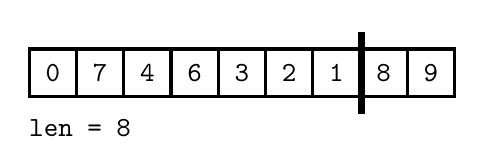
\begin{tikzpicture}

\draw (0.3, -0.3)
  node[draw, line width=0.04cm, , color=black,
       rounded corners=0cm, inner sep=0cm] {

\begin{minipage}[t][0.6cm]{0.6cm}
\mbox{}

\end{minipage}

};\draw (0.3, -0.3) node[color=black] {{\texttt{0}}};
\draw (0.8999999999999999, -0.3)
  node[draw, line width=0.04cm, , color=black,
       rounded corners=0cm, inner sep=0cm] {

\begin{minipage}[t][0.6cm]{0.6cm}
\mbox{}

\end{minipage}

};\draw (0.8999999999999999, -0.3) node[color=black] {{\texttt{7}}};
\draw (1.5, -0.3)
  node[draw, line width=0.04cm, , color=black,
       rounded corners=0cm, inner sep=0cm] {

\begin{minipage}[t][0.6cm]{0.6cm}
\mbox{}

\end{minipage}

};\draw (1.5, -0.3) node[color=black] {{\texttt{4}}};
\draw (2.0999999999999996, -0.3)
  node[draw, line width=0.04cm, , color=black,
       rounded corners=0cm, inner sep=0cm] {

\begin{minipage}[t][0.6cm]{0.6cm}
\mbox{}

\end{minipage}

};\draw (2.0999999999999996, -0.3) node[color=black] {{\texttt{6}}};
\draw (2.7, -0.3)
  node[draw, line width=0.04cm, , color=black,
       rounded corners=0cm, inner sep=0cm] {

\begin{minipage}[t][0.6cm]{0.6cm}
\mbox{}

\end{minipage}

};\draw (2.7, -0.3) node[color=black] {{\texttt{3}}};
\draw (3.3, -0.3)
  node[draw, line width=0.04cm, , color=black,
       rounded corners=0cm, inner sep=0cm] {

\begin{minipage}[t][0.6cm]{0.6cm}
\mbox{}

\end{minipage}

};\draw (3.3, -0.3) node[color=black] {{\texttt{2}}};
\draw (3.9, -0.3)
  node[draw, line width=0.04cm, , color=black,
       rounded corners=0cm, inner sep=0cm] {

\begin{minipage}[t][0.6cm]{0.6cm}
\mbox{}

\end{minipage}

};\draw (3.9, -0.3) node[color=black] {{\texttt{1}}};
\draw (4.5, -0.3)
  node[draw, line width=0.04cm, , color=black,
       rounded corners=0cm, inner sep=0cm] {

\begin{minipage}[t][0.6cm]{0.6cm}
\mbox{}

\end{minipage}

};\draw (4.5, -0.3) node[color=black] {{\texttt{8}}};
\draw (5.1, -0.3)
  node[draw, line width=0.04cm, , color=black,
       rounded corners=0cm, inner sep=0cm] {

\begin{minipage}[t][0.6cm]{0.6cm}
\mbox{}

\end{minipage}

};\draw (5.1, -0.3) node[color=black] {{\texttt{9}}};\draw[line width=0.1cm,black] (4.22,-0.82) to  (4.22,0.22);

\draw (1.0, -1.0)
  node[draw=none, line width=0cm, , color=black,
       rounded corners=0cm, inner sep=0cm] {

\begin{minipage}[t][0.1cm]{2cm}
\mbox{}

\end{minipage}

};
\draw (1.0, -1.0) node[color=black,
 inner sep=0cm] {
 
\begin{minipage}[t][0.1cm]{2cm}
\texttt{len = 8}
\end{minipage}

};
\end{tikzpicture}

\end{center}



The tree is clearly not balanced at \verb!4!: the left height us 1
and the right height is -1.
I'm going to perform a left rotation about \verb!4!:
\begin{center}
\begin{tikzpicture}

\fill[white] (0.0, 0.0) circle (0.3);
\node [line width=0.03cm,black,minimum size=0.57cm,draw,circle] at (0.0,0.0)(10){};\draw (0.0, 0.0) node[color=black] {\texttt{10}};
\fill[white] (-3.0, -1.0) circle (0.3);
\node [line width=0.03cm,black,minimum size=0.57cm,draw,circle] at (-3.0,-1.0)(2){};\draw (-3.0, -1.0) node[color=black] {\texttt{2}};
\fill[white] (3.0, -1.0) circle (0.3);
\node [line width=0.03cm,black,minimum size=0.57cm,draw,circle] at (3.0,-1.0)(18){};\draw (3.0, -1.0) node[color=black] {\texttt{18}};
\fill[white] (-4.5, -2.0) circle (0.3);
\node [line width=0.03cm,black,minimum size=0.57cm,draw,circle] at (-4.5,-2.0)(0){};\draw (-4.5, -2.0) node[color=black] {\texttt{0}};
\fill[white] (-1.5, -2.0) circle (0.3);
\node [line width=0.03cm,black,minimum size=0.57cm,draw,circle] at (-1.5,-2.0)(4){};\draw (-1.5, -2.0) node[color=black] {\texttt{4}};
\fill[white] (1.5, -2.0) circle (0.3);
\node [line width=0.03cm,black,minimum size=0.57cm,draw,circle] at (1.5,-2.0)(17){};\draw (1.5, -2.0) node[color=black] {\texttt{17}};
\fill[white] (4.5, -2.0) circle (0.3);
\node [line width=0.03cm,black,minimum size=0.57cm,draw,circle] at (4.5,-2.0)(20){};\draw (4.5, -2.0) node[color=black] {\texttt{20}};
\fill[white] (-2.25, -3.0) circle (0.3);
\node [line width=0.03cm,black,minimum size=0.57cm,draw,circle] at (-2.25,-3.0)(3){};\draw (-2.25, -3.0) node[color=black] {\texttt{3}};\draw[line width=0.03cm,black,->,>=triangle 60] (10) to  (2);
\draw[line width=0.03cm,black,->,>=triangle 60] (10) to  (18);
\draw[line width=0.03cm,black,->,>=triangle 60] (4) to  (3);
\draw[line width=0.03cm,black,->,>=triangle 60] (2) to  (0);
\draw[line width=0.03cm,black,->,>=triangle 60] (2) to  (4);
\draw[line width=0.03cm,black,->,>=triangle 60] (18) to  (17);
\draw[line width=0.03cm,black,->,>=triangle 60] (18) to  (20);
\end{tikzpicture}

\end{center}




Note that the tree is now height--balanced.


\newpage
\subsection{Height changes due to rotations}

Now let's analyze the general case.

Let $T$ be the subtree tree with root $\alpha$
before the rotation and $\operatorname{LEFT}(T)$
be this subtree after.
The following are the relevant heights before and after
left rotation about node $\alpha$:
\begin{align*}
  \operatorname{height}(T) &=
  1 +
  \max(\operatorname{height}(T_1),
  1 + \max(\operatorname{height}(T_2), \operatorname{height}(T_3)))
  \\
  \operatorname{height}(\operatorname{LEFT}(T)) &=
  1 + \max(1+\max(\operatorname{height}(T_1),\operatorname{height}(T_2)),
  \operatorname{height}(T_3)))
\end{align*}
or, to make it easier to read, if I write $h_i$ for
$\operatorname{height}(T_i)$, then
\begin{align*}
  \operatorname{height}(T) &=
  1 +
  \max(h_1,
  1 + \max(h_2, h_3))
  \\
  \operatorname{height}(\operatorname{LEFT}(T)) &=
  1 + \max(1+\max(h_1,h_2),h_3)
\end{align*}
So it the heights are $h_1=2, h_2=1, h_3=3$, then
\begin{align*}
  \operatorname{height}(T) &=
  1 +
  \max(2,
  1 + \max(1, 3)) = 1 + \max(2, 4)
  \\
  \operatorname{height}(\operatorname{LEFT}(T)) &=
  1 + \max(1+\max(2,1),3)
  = 1 + \max(3, 3)
\end{align*}
For the pre-left-rotation case, you see that the two subtrees of $\alpha$
have
heights 2 and 4 and is therefore unbalanced.
After rotation, the two subtrees of $\beta$ has heights $3$ and $3$ is
balanced.


Suppose you have added a node with value $k$ into a BST
and it become unbalanced.
It should be clear unbalanced nodes (if any)
must be along the path that $k$ takes within the tree
as it finds its place of insertion.
When you go from the inserted new node back to the root,
suppose the first node that is unbalanced is $\alpha$:

\begin{center}

\begin{tikzpicture}
\node at (3,-0.8) [minimum size=8mm] (E) {$$};
\node at (2,-2.4000000000000004) [circle,draw,minimum size=8mm] (A) {$\alpha$};
\node at (0,-3.2)
    [isosceles triangle, shape border rotate=+90,
     draw,minimum size=8mm,minimum height=2cm,
     anchor=north] (Ctriangle) {$T_1$};
\coordinate (C) at (0,-3.2);
\node at (4,-3.2)
    [isosceles triangle, shape border rotate=+90,
     draw,minimum size=8mm,minimum height=2cm,
     anchor=north] (Btriangle) {$T_2$};
\coordinate (B) at (4,-3.2);
\draw [-,thick] (A) -- (B);
\draw [-,thick] (A) -- (C);
\draw [-,thick] (E) -- (A);

;
\end{tikzpicture}
    
\end{center}



\underline{CASE LEFT: 
$k$ is inserted into the left subtree of $\alpha$.}
\input{stdout71.tex}
Of course before adding $k$, $\alpha$ is balanced:
\[
h(T_1) = h(T_2) + \ep
\]
where $\ep = -1, 0, 1$.
Since $\alpha$ is unbalanced  after adding $k$, we must have
\[
h(T_1 + k) = h(T_2) + 2
\]
(the 2 on the right can't be more than 2, right?)
and 
\[
h(T_1) = h(T_2) + 1
\]
This implies that $T_1$ must have at least one node.
So let me draw the tree, before inserting $k$, at $\alpha$ like this:

\begin{center}

\begin{tikzpicture}
\node at (4,-0.8) [minimum size=8mm] (E) {$$};
\node at (3,-2.4000000000000004) [circle,draw,minimum size=8mm] (A) {$\alpha$};
\node at (1,-3.2) [circle,draw,minimum size=8mm] (C) {$\beta$};
\node at (5,-3.2)
    [isosceles triangle, shape border rotate=+90,
     draw,minimum size=8mm,
     anchor=north] (Btriangle) {$T'_3$};
\coordinate (B) at (5,-3.2);
\node at (0,-4.0)
    [isosceles triangle, shape border rotate=+90,
     draw,minimum size=8mm,
     anchor=north] (Dtriangle) {$T'_1$};
\coordinate (D) at (0,-4.0);
\node at (2,-4.0)
    [isosceles triangle, shape border rotate=+90,
     draw,minimum size=8mm,
     anchor=north] (Ftriangle) {$T'_2$};
\coordinate (F) at (2,-4.0);
\draw [-,thick] (A) -- (B);
\draw [-,thick] (A) -- (C);
\draw [-,thick] (E) -- (A);
\draw [-,thick] (C) -- (D);
\draw [-,thick] (C) -- (F);

;
\end{tikzpicture}
    
\end{center}


Tying this to the previous diagram, 
we have
\[
1 + \max(h(T'_1), h(T'_2)) = h(T'_3) + 1
\]
i.e., 
\[
\max(h(T'_1), h(T'_2)) = h(T'_3)
\]

\underline{CASE LEFT-LEFT: $k$ is inserted into the 
left subtree of the left subtree of $\alpha$.}
Here's the picture:
\input{stdout73.tex}
I claim that
\[
h(T'_1) = h(T'_2) = h(T'_3) 
\]


By our assumption, this makes the tree unbalanced by $\alpha$.
We had this before adding $k$:
\[
\max(h(T'_1), h(T'_2)) = h(T'_3)
\]
On adding $k$ for this case, i.e., to $T_1'$, 
$\alpha$ becomes unbalanced.
Therefore
\[
h(T'_1 + k) = h(T'_1) + 1,
\,\,\,\,\,
h(T'_1) \geq h(T'_2)
\]
That means that 
\[
h(T'_1) = h(T'_3)
\]
Note also that if $h(T'_1) > h(T'_2)$,
then when $k$ is added to $T'_1$, the resulting
tree is unbalanced at $\beta$
which contradicts out assumption that 
the resulting tree is unbalanced at $\alpha$.
Hence we must have $h(T'_1) = h(T'_2)$.
Altogether we have 
\[
h(T'_1) = h(T'_2) = h(T'_3)
\] 

I right--rotate at $\alpha$ to get this:
\input{stdout74.tex}
The height of the left subtree of $\beta$ is $h(T'_1) + 1$
and the height of the right subtree at 
$\beta$ is $1 + \max(h(T'_2), h(T'_3)) = 1 + h(T'_1)$.
Therefore this resulting tree is balanced at $\beta$.

Note for the original tree, before inserting $k$
and when the tree was balanced,
\input{stdout75.tex}
the height at $\alpha$ is $h(T_1') + 2$.
After inserting $k$ and the right rotation:
\input{stdout76.tex}
the height at $\beta$ is also $h(T'_1)+2$.
This means that the whole tree must be balanced.



\underline{CASE LEFT-RIGHT: $k$ is inserted into the 
  right subtree of the left subtree of $\alpha$.}
\input{stdout77.tex}
Let's look at $h(T'_1)$ and $h(T'_2)$.
Since $\beta$ is balanced, they are at most one away.
So $h(T'_2) = h(T'_1) + \ep$, $\ep = -1, 0, 1$.
If $\ep = -1$, then $T'_2$ is one shorter than
$T'_1$. In that case inserting $k$ into $T_2$
will mean that the height of $T_2$ will either
remain the same or increase by 1
which implies that the height at $\beta$
is unchanged.
This means that $\alpha$ cannot become unbalanced
after the insertion of $k$.
Also, $\ep$ cannot be 1 otherwise
after inserting $k$, $\beta$ becomes unbalanced
which contradicts the fact that the $\alpha$
is the lowest node to be unbalanced when $k$ is inserted.
Therefore $\ep$ must be $0$:
$h(T'_1) = h(T'_2)$.

Since adding $k$ to $T'_2$ unbalances $\alpha$, 
the lowest node of $T'_3$ must be 2 away from $k$ after it's inserted into 
$T'_2$.
Since $T'_2$ is one below $\beta$,
we must have $h(T'_2) = h(T'_3)$.

Therefore altogether $h(T'_1) = h(T'_2) = h(T'_3)$.

Look at this:

\begin{center}

\begin{tikzpicture}
\node at (3,-0.8) [minimum size=8mm] (E) {$$};
\node at (2,-2.4000000000000004) [circle,draw,minimum size=8mm] (C) {$\beta$};
\node at (0,-3.2)
    [isosceles triangle, shape border rotate=+90,
     draw,minimum size=8mm,
     anchor=north] (Dtriangle) {$T'_1$};
\coordinate (D) at (0,-3.2);
\node at (4,-3.2) [circle,draw,minimum size=8mm] (A) {$\alpha$};
\node at (2,-4.0)
    [isosceles triangle, shape border rotate=+90,
     draw,minimum size=8mm,
     anchor=north] (Ftriangle) {$T'_2+k$};
\coordinate (F) at (2,-4.0);
\node at (6,-4.0)
    [isosceles triangle, shape border rotate=+90,
     draw,minimum size=8mm,
     anchor=north] (Btriangle) {$T'_3$};
\coordinate (B) at (6,-4.0);
\draw [-,thick] (E) -- (C);
\draw [-,thick] (C) -- (D);
\draw [-,thick] (C) -- (A);
\draw [-,thick] (A) -- (F);
\draw [-,thick] (A) -- (B);

;
\end{tikzpicture}
    
\end{center}


This is NOT the right \lq\lq rotation".
(Find an example on your own to prove what I just said.)

The right thing to do is to do a \textit{left} rotation
at $\beta$ so that $\beta$ is \lq\lq heavier"
on the left and then then do a right rotation at $\alpha$.
Let me show you.
We start here where $k$ is now in $T''_2$ or $T''_3$:

\begin{center}

\begin{tikzpicture}
\node at (5,-0.8) [minimum size=8mm] (E) {$$};
\node at (4,-2.4000000000000004) [circle,draw,minimum size=8mm] (A) {$\alpha$};
\node at (2,-3.2) [circle,draw,minimum size=8mm] (C) {$\beta$};
\node at (6,-3.2)
    [isosceles triangle, shape border rotate=+90,
     draw,minimum size=8mm,
     anchor=north] (Btriangle) {$T''_4$};
\coordinate (B) at (6,-3.2);
\node at (0,-4.0)
    [isosceles triangle, shape border rotate=+90,
     draw,minimum size=8mm,
     anchor=north] (Dtriangle) {$T''_1$};
\coordinate (D) at (0,-4.0);
\node at (3,-4.0) [circle,draw,minimum size=8mm] (F) {$\gamma$};
\node at (2,-4.800000000000001)
    [isosceles triangle, shape border rotate=+90,
     draw,minimum size=8mm,
     anchor=north] (Gtriangle) {$T''_2$};
\coordinate (G) at (2,-4.800000000000001);
\node at (4,-4.800000000000001)
    [isosceles triangle, shape border rotate=+90,
     draw,minimum size=8mm,
     anchor=north] (Htriangle) {$T''_3$};
\coordinate (H) at (4,-4.800000000000001);
\draw [-,thick] (A) -- (B);
\draw [-,thick] (A) -- (C);
\draw [-,thick] (E) -- (A);
\draw [-,thick] (C) -- (D);
\draw [-,thick] (C) -- (F);
\draw [-,thick] (F) -- (G);
\draw [-,thick] (F) -- (H);

;
\end{tikzpicture}
    
\end{center}


After a left rotation at $\beta$, I get this:

\begin{center}

\begin{tikzpicture}
\node at (7,-0.8) [minimum size=8mm] (E) {$$};
\node at (5,-2.4000000000000004) [circle,draw,minimum size=8mm] (A) {$\alpha$};
\node at (3,-3.2) [circle,draw,minimum size=8mm] (F) {$\gamma$};
\node at (7,-3.2)
    [isosceles triangle, shape border rotate=+90,
     draw,minimum size=8mm,
     anchor=north] (Btriangle) {$T''_4$};
\coordinate (B) at (7,-3.2);
\node at (1,-4.0) [circle,draw,minimum size=8mm] (C) {$\beta$};
\node at (4,-4.0)
    [isosceles triangle, shape border rotate=+90,
     draw,minimum size=8mm,
     anchor=north] (Htriangle) {$T''_3$};
\coordinate (H) at (4,-4.0);
\node at (0,-4.800000000000001)
    [isosceles triangle, shape border rotate=+90,
     draw,minimum size=8mm,
     anchor=north] (Dtriangle) {$T''_1$};
\coordinate (D) at (0,-4.800000000000001);
\node at (2,-4.800000000000001)
    [isosceles triangle, shape border rotate=+90,
     draw,minimum size=8mm,
     anchor=north] (Gtriangle) {$T''_2$};
\coordinate (G) at (2,-4.800000000000001);
\draw [-,thick] (E) -- (A);
\draw [-,thick] (A) -- (F);
\draw [-,thick] (A) -- (B);
\draw [-,thick] (F) -- (C);
\draw [-,thick] (F) -- (H);
\draw [-,thick] (C) -- (D);
\draw [-,thick] (C) -- (G);
\draw [-,thick] (A) -- (B);

;
\end{tikzpicture}
    
\end{center}


Now I right rotation at $\alpha$ to get this:

\begin{center}

\begin{tikzpicture}
\node at (5,-0.8) [minimum size=8mm] (E) {$$};
\node at (3,-2.4000000000000004) [circle,draw,minimum size=8mm] (F) {$\gamma$};
\node at (1,-3.2) [circle,draw,minimum size=8mm] (C) {$\beta$};
\node at (5,-3.2) [circle,draw,minimum size=8mm] (A) {$\alpha$};
\node at (0,-4.0)
    [isosceles triangle, shape border rotate=+90,
     draw,minimum size=8mm,
     anchor=north] (Dtriangle) {$T''_1$};
\coordinate (D) at (0,-4.0);
\node at (2,-4.0)
    [isosceles triangle, shape border rotate=+90,
     draw,minimum size=8mm,
     anchor=north] (Gtriangle) {$T''_2$};
\coordinate (G) at (2,-4.0);
\node at (4,-4.0)
    [isosceles triangle, shape border rotate=+90,
     draw,minimum size=8mm,
     anchor=north] (Htriangle) {$T''_3$};
\coordinate (H) at (4,-4.0);
\node at (6,-4.0)
    [isosceles triangle, shape border rotate=+90,
     draw,minimum size=8mm,
     anchor=north] (Btriangle) {$T''_4$};
\coordinate (B) at (6,-4.0);
\draw [-,thick] (E) -- (F);
\draw [-,thick] (F) -- (C);
\draw [-,thick] (F) -- (A);
\draw [-,thick] (C) -- (D);
\draw [-,thick] (C) -- (G);
\draw [-,thick] (A) -- (H);
\draw [-,thick] (A) -- (B);

;
\end{tikzpicture}
    
\end{center}



Let me summarize.
Suppose after inserting a node $k$ into a BST,
$\alpha$ is the lower node that is unbalanced.
\begin{tightlist}
\li LEFT-LEFT CASE: If $k$ took a left-left direction from $\alpha$,
then you should do a right rotation.
\li LEFT-RIGHT: If $k$ took at left-right direction from $\alpha$,
then you should a left rotation on the left child $\beta$ of $\alpha$
followed by a right rotation at $\beta$ which occupies the original 
position of $\alpha$.
\end{tightlist}

If should not be too surprising that the mirror image of
the above is true:
Suppose after inserting a node $k$ into a BST,
$\alpha$ is the lower node that is unbalanced.
\begin{tightlist}
\li RIGHT-RIGHT CASE: If $k$ took a right-right direction from $\alpha$,
then you should do a left rotation.
\li RIGHT-LEFT: If $k$ took at right-left direction from $\alpha$,
then you should a right rotation on the right child $\beta$ of $\alpha$
followed by a left rotation at $\beta$ which occupies the original 
position of $\alpha$.
\end{tightlist}
Draw a picture similar to the above to see what's happening.

\newpage
\subsection{AVL trees}

An AVL tree $T$ is a tree that is self-balancing BST in the sense that
the insert and delete operations include self-balancing operations
(using left and right rotations) so that the tree is balanced after each
insert or delete operation.

\newpage
\subsection{AVL insert}
Suppose a node $n$ is inserted into $T$.
Suppose the new tree is $T'$.
There's a path from the root of $T'$ to $n$.
You go up along this path and when you are at a node $m$
that is unbalanced (i.e., the subtree with $m$ as root
is unbalanced), we balance at $m$:
\begin{tightlist}
  \li CASE: left-left. If the path from $m$ along $P$ going down to the new node is
  left-left,
  you perform a right rotation at $m$.
  \li CASE: left-right. If the path from $m$ along $P$ going down to the new node is
  left-right,
  you perform a left rotation one step below $m$ and then a right rotation at $m$.
  \li CASE: right-right. If the path from $m$ along $P$ going down to the new node is
  right-right,
  you perform a left rotation at $m$.
  \li CASE: right-left. If the path from $m$ along $P$ going down to the new node is
  right-left,
  you perform a right rotation one step below $m$ and then a left rotation at $m$.
\end{tightlist}

For instance suppose I start off with this:

\begin{center}
\begin{tikzpicture}

\fill[white] (0.0, 0.0) circle (0.3);
\node [line width=0.03cm,black,minimum size=0.57cm,draw,circle] at (0.0,0.0)(10){};\draw (0.0, 0.0) node[color=black] {\texttt{10}};
\fill[white] (-0.75, -1.0) circle (0.3);
\node [line width=0.03cm,black,minimum size=0.57cm,draw,circle] at (-0.75,-1.0)(5){};\draw (-0.75, -1.0) node[color=black] {\texttt{5}};
\fill[white] (0.75, -1.0) circle (0.3);
\node [line width=0.03cm,black,minimum size=0.57cm,draw,circle] at (0.75,-1.0)(18){};\draw (0.75, -1.0) node[color=black] {\texttt{18}};\draw[line width=0.03cm,black,->,>=triangle 60] (10) to  (5);
\draw[line width=0.03cm,black,->,>=triangle 60] (10) to  (18);
\end{tikzpicture}

\end{center}



This is height balanced.
After I insert 2, I get:

\begin{center}
\begin{tikzpicture}

\fill[white] (0.0, 0.0) circle (0.3);
\node [line width=0.03cm,black,minimum size=0.57cm,draw,circle] at (0.0,0.0)(10){};\draw (0.0, 0.0) node[color=black] {\texttt{10}};
\fill[white] (-1.5, -1.0) circle (0.3);
\node [line width=0.03cm,black,minimum size=0.57cm,draw,circle] at (-1.5,-1.0)(5){};\draw (-1.5, -1.0) node[color=black] {\texttt{5}};
\fill[white] (1.5, -1.0) circle (0.3);
\node [line width=0.03cm,black,minimum size=0.57cm,draw,circle] at (1.5,-1.0)(18){};\draw (1.5, -1.0) node[color=black] {\texttt{18}};
\fill[white] (-2.25, -2.0) circle (0.3);
\node [line width=0.03cm,black,minimum size=0.57cm,draw,circle] at (-2.25,-2.0)(2){};\draw (-2.25, -2.0) node[color=black] {\texttt{2}};\draw[line width=0.03cm,black,->,>=triangle 60] (10) to  (5);
\draw[line width=0.03cm,black,->,>=triangle 60] (10) to  (18);
\draw[line width=0.03cm,black,->,>=triangle 60] (5) to  (2);
\end{tikzpicture}

\end{center}



Checking all the nodes along the insertion path,
I see that they are all balanced.
(Make sure you check that.)
Now if I insert a 0, I get this:

\begin{center}
\begin{tikzpicture}

\fill[blue!10] (0.0, 0.0) circle (0.35);
\node [line width=0.03cm,black,minimum size=0.6699999999999999cm,draw,circle] at (0.0,0.0)(1){};\draw (0.0, 0.0) node[color=black] {\texttt{1}};
\fill[blue!10] (-1.9, -1.0) circle (0.35);
\node [line width=0.03cm,black,minimum size=0.6699999999999999cm,draw,circle] at (-1.9,-1.0)(0){};\draw (-1.9, -1.0) node[color=black] {\texttt{0}};
\fill[blue!10] (1.9, -1.0) circle (0.35);
\node [line width=0.03cm,black,minimum size=0.6699999999999999cm,draw,circle] at (1.9,-1.0)(2){};\draw (1.9, -1.0) node[color=black] {\texttt{2}};
\fill[blue!10] (-2.85, -2.0) circle (0.35);
\node [line width=0.03cm,black,minimum size=0.6699999999999999cm,draw,circle] at (-2.85,-2.0)(3){};\draw (-2.85, -2.0) node[color=black] {\texttt{3}};
\fill[blue!10] (-0.95, -2.0) circle (0.35);
\node [line width=0.03cm,black,minimum size=0.6699999999999999cm,draw,circle] at (-0.95,-2.0)(4){};\draw (-0.95, -2.0) node[color=black] {\texttt{4}};
\fill[blue!10] (0.95, -2.0) circle (0.35);
\node [line width=0.03cm,black,minimum size=0.6699999999999999cm,draw,circle] at (0.95,-2.0)(6){};\draw (0.95, -2.0) node[color=black] {\texttt{6}};
\fill[blue!10] (2.85, -2.0) circle (0.35);
\node [line width=0.03cm,black,minimum size=0.6699999999999999cm,draw,circle] at (2.85,-2.0)(7){};\draw (2.85, -2.0) node[color=black] {\texttt{7}};
\fill[blue!10] (-3.33, -3.0) circle (0.35);
\node [line width=0.03cm,black,minimum size=0.6699999999999999cm,draw,circle] at (-3.33,-3.0)(8){};\draw (-3.33, -3.0) node[color=black] {\texttt{8}};
\fill[blue!10] (-2.38, -3.0) circle (0.35);
\node [line width=0.03cm,black,minimum size=0.6699999999999999cm,draw,circle] at (-2.38,-3.0)(9){};\draw (-2.38, -3.0) node[color=black] {\texttt{9}};\draw[line width=0.03cm,black] (1) to  (0);
\draw[line width=0.03cm,black] (1) to  (2);
\draw[line width=0.03cm,black] (0) to  (3);
\draw[line width=0.03cm,black] (0) to  (4);
\draw[line width=0.03cm,black] (2) to  (6);
\draw[line width=0.03cm,black] (2) to  (7);
\draw[line width=0.03cm,black] (3) to  (8);
\draw[line width=0.03cm,black] (3) to  (9);

\fill[red!10] (-2.38, -3.0) circle (0.35);
\draw[line width=0.03cm,black] (-2.38, -3.0) circle (0.33499999999999996);\draw (-2.38, -3.0) node[color=black] {9};
\fill[red!10] (-3.33, -3.0) circle (0.35);
\draw[line width=0.03cm,black] (-3.33, -3.0) circle (0.33499999999999996);\draw (-3.33, -3.0) node[color=black] {8};
\fill[red!10] (2.85, -2.0) circle (0.35);
\draw[line width=0.03cm,black] (2.85, -2.0) circle (0.33499999999999996);\draw (2.85, -2.0) node[color=black] {7};
\fill[red!10] (0.95, -2.0) circle (0.35);
\draw[line width=0.03cm,black] (0.95, -2.0) circle (0.33499999999999996);\draw (0.95, -2.0) node[color=black] {6};
\fill[red!10] (-0.95, -2.0) circle (0.35);
\draw[line width=0.03cm,black] (-0.95, -2.0) circle (0.33499999999999996);\draw (-0.95, -2.0) node[color=black] {4};
\fill[red!10] (-2.85, -2.0) circle (0.35);
\draw[line width=0.03cm,black] (-2.85, -2.0) circle (0.33499999999999996);\draw (-2.85, -2.0) node[color=black] {3};
\fill[red!10] (1.9, -1.0) circle (0.35);
\draw[line width=0.03cm,black] (1.9, -1.0) circle (0.33499999999999996);\draw (1.9, -1.0) node[color=black] {2};\draw[line width=0.1cm,white] (1) to  (2);
\draw[line width=0.03cm,black,,dashed] (1) to  (2);
\draw[line width=0.1cm,white] (3) to  (9);
\draw[line width=0.03cm,black,,dashed] (3) to  (9);
\draw[line width=0.1cm,white] (3) to  (8);
\draw[line width=0.03cm,black,,dashed] (3) to  (8);
\draw[line width=0.1cm,white] (2) to  (7);
\draw[line width=0.03cm,black,,dashed] (2) to  (7);
\draw[line width=0.1cm,white] (2) to  (6);
\draw[line width=0.03cm,black,,dashed] (2) to  (6);
\draw[line width=0.1cm,white] (0) to  (4);
\draw[line width=0.03cm,black,,dashed] (0) to  (4);
\draw[line width=0.1cm,white] (0) to  (3);
\draw[line width=0.03cm,black,,dashed] (0) to  (3);
\end{tikzpicture}

\end{center}



The path of insertion is in red.

When I go back up the tree from the new node, I see that
the first node that is not balanced is 5:

\begin{center}
\begin{tikzpicture}

\fill[white] (0.0, 0.0) circle (0.3);
\node [line width=0.03cm,black,minimum size=0.57cm,draw,circle] at (0.0,0.0)(10){};\draw (0.0, 0.0) node[color=black] {\texttt{10}};
\fill[white] (-3.0, -1.0) circle (0.35);
\node [line width=0.1cm,red,minimum size=0.6cm,draw,circle] at (-3.0,-1.0)(5){};\draw (-3.0, -1.0) node[color=black] {\texttt{5}};
\fill[white] (3.0, -1.0) circle (0.3);
\node [line width=0.03cm,black,minimum size=0.57cm,draw,circle] at (3.0,-1.0)(18){};\draw (3.0, -1.0) node[color=black] {\texttt{18}};
\fill[white] (-4.5, -2.0) circle (0.3);
\node [line width=0.03cm,black,minimum size=0.57cm,draw,circle] at (-4.5,-2.0)(2){};\draw (-4.5, -2.0) node[color=black] {\texttt{2}};
\fill[white] (-5.25, -3.0) circle (0.3);
\node [line width=0.03cm,black,minimum size=0.57cm,draw,circle] at (-5.25,-3.0)(0){};\draw (-5.25, -3.0) node[color=black] {\texttt{0}};\draw[line width=0.03cm,black,->,>=triangle 60] (10) to  (5);
\draw[line width=0.03cm,black,->,>=triangle 60] (10) to  (18);
\draw[line width=0.1cm,red,->,>=triangle 60] (5) to  (2);
\draw[line width=0.1cm,red,->,>=triangle 60] (2) to  (0);
\end{tikzpicture}

\end{center}



Along this path, at 5, I took two lefts down -- we are in the left-left case.
Therefore I will perform a right rotation at 5 to get:

\begin{center}
\begin{tikzpicture}

\fill[white] (0.0, 0.0) circle (0.3);
\node [line width=0.03cm,black,minimum size=0.57cm,draw,circle] at (0.0,0.0)(10){};\draw (0.0, 0.0) node[color=black] {\texttt{10}};
\fill[white] (-1.5, -1.0) circle (0.35);
\node [line width=0.1cm,red,minimum size=0.6cm,draw,circle] at (-1.5,-1.0)(2){};\draw (-1.5, -1.0) node[color=black] {\texttt{2}};
\fill[white] (1.5, -1.0) circle (0.3);
\node [line width=0.03cm,black,minimum size=0.57cm,draw,circle] at (1.5,-1.0)(18){};\draw (1.5, -1.0) node[color=black] {\texttt{18}};
\fill[white] (-2.25, -2.0) circle (0.3);
\node [line width=0.03cm,black,minimum size=0.57cm,draw,circle] at (-2.25,-2.0)(0){};\draw (-2.25, -2.0) node[color=black] {\texttt{0}};
\fill[white] (-0.75, -2.0) circle (0.3);
\node [line width=0.03cm,black,minimum size=0.57cm,draw,circle] at (-0.75,-2.0)(5){};\draw (-0.75, -2.0) node[color=black] {\texttt{5}};\draw[line width=0.03cm,black,->,>=triangle 60] (10) to  (2);
\draw[line width=0.03cm,black,->,>=triangle 60] (10) to  (18);
\draw[line width=0.03cm,black,->,>=triangle 60] (2) to  (0);
\draw[line width=0.03cm,black,->,>=triangle 60] (2) to  (5);
\end{tikzpicture}

\end{center}



The tree is now balanced at 2 (the previous location of 5).
it's also balanced at 10.

If I insert a 3, I get this:

\begin{center}
\begin{tikzpicture}

\fill[white] (0.0, 0.0) circle (0.3);
\node [line width=0.03cm,black,minimum size=0.57cm,draw,circle] at (0.0,0.0)(10){};\draw (0.0, 0.0) node[color=black] {\texttt{10}};
\fill[white] (-3.0, -1.0) circle (0.3);
\node [line width=0.03cm,black,minimum size=0.57cm,draw,circle] at (-3.0,-1.0)(2){};\draw (-3.0, -1.0) node[color=black] {\texttt{2}};
\fill[white] (3.0, -1.0) circle (0.3);
\node [line width=0.03cm,black,minimum size=0.57cm,draw,circle] at (3.0,-1.0)(18){};\draw (3.0, -1.0) node[color=black] {\texttt{18}};
\fill[white] (-4.5, -2.0) circle (0.3);
\node [line width=0.03cm,black,minimum size=0.57cm,draw,circle] at (-4.5,-2.0)(0){};\draw (-4.5, -2.0) node[color=black] {\texttt{0}};
\fill[white] (-1.5, -2.0) circle (0.3);
\node [line width=0.03cm,black,minimum size=0.57cm,draw,circle] at (-1.5,-2.0)(5){};\draw (-1.5, -2.0) node[color=black] {\texttt{5}};
\fill[white] (-2.25, -3.0) circle (0.3);
\node [line width=0.03cm,black,minimum size=0.57cm,draw,circle] at (-2.25,-3.0)(3){};\draw (-2.25, -3.0) node[color=black] {\texttt{3}};\draw[line width=0.1cm,red,->,>=triangle 60] (10) to  (2);
\draw[line width=0.03cm,black,->,>=triangle 60] (10) to  (18);
\draw[line width=0.03cm,black,->,>=triangle 60] (2) to  (0);
\draw[line width=0.1cm,red,->,>=triangle 60] (2) to  (5);
\draw[line width=0.1cm,red,->,>=triangle 60] (5) to  (3);
\end{tikzpicture}

\end{center}



The part of insertion is shown in red.
Going up along the path of insertion, the first node that is unbalanced
is 10.
At 10, going down, I take a left (at 10) then a right (at 2).
Therefore, I will first make a left rotation at 2, and then a right rotation at 10.
The left rotation at 2 gives me this:


\begin{center}

\begin{tikzpicture}
\node at (8,-1) [circle,draw,minimum size=8mm] (A) {\texttt{34}};
\node at (4,-2) [circle,draw,minimum size=8mm] (B) {\texttt{28}};
\node at (12,-2) [circle,draw,minimum size=8mm] (C) {\texttt{16}};
\node at (2,-3) [circle,draw,minimum size=8mm] (D) {\texttt{23}};
\node at (6,-3) [circle,draw,minimum size=8mm] (E) {\texttt{25}};
\node at (10,-3) [circle,draw,minimum size=8mm] (F) {\texttt{13}};
\node at (14,-3) [circle,draw,minimum size=8mm] (G) {\texttt{7}};
\node at (1,-4) [circle,draw,minimum size=8mm] (H) {\texttt{10}};
\node at (3,-4) [circle,draw,minimum size=8mm] (I) {\texttt{8}};
\node at (5,-4) [circle,draw,minimum size=8mm] (J) {\texttt{24}};
\node at (7,-4) [circle,draw,minimum size=8mm] (K) {\texttt{14}};
\node at (9,-4) [circle,draw,minimum size=8mm] (L) {\texttt{3}};
\node at (11,-4) [circle,draw,minimum size=8mm] (M) {\texttt{9}};
\node at (13,-4) [circle,draw,minimum size=8mm] (N) {\texttt{5}};
\node at (15,-4) [circle,draw,minimum size=8mm] (O) {\texttt{4}};
\node at (0,-5) [circle,draw,minimum size=8mm] (P) {\texttt{9}};
\draw [-,thick] (A) -- (B);
\draw [-,thick] (A) -- (C);
\draw [-,thick] (B) -- (D);
\draw [-,thick] (B) -- (E);
\draw [-,thick] (C) -- (G);
\draw [-,thick] (C) -- (F);
\draw [-,thick] (D) -- (H);
\draw [-,thick] (D) -- (I);
\draw [-,thick] (E) -- (J);
\draw [-,thick] (E) -- (K);
\draw [-,thick] (F) -- (L);
\draw [-,thick] (F) -- (M);
\draw [-,thick] (G) -- (N);
\draw [-,thick] (G) -- (O);
\draw [-,thick] (H) -- (P);

;
\end{tikzpicture}
    
\end{center}



and then I do a right rotation at 10:

\begin{center}
\begin{tikzpicture}

\fill[white] (0.0, 0.0) circle (0.3);
\node [line width=0.03cm,black,minimum size=0.57cm,draw,circle] at (0.0,0.0)(5){};\draw (0.0, 0.0) node[color=black] {\texttt{5}};
\fill[white] (-1.5, -1.0) circle (0.3);
\node [line width=0.03cm,black,minimum size=0.57cm,draw,circle] at (-1.5,-1.0)(2){};\draw (-1.5, -1.0) node[color=black] {\texttt{2}};
\fill[white] (1.5, -1.0) circle (0.3);
\node [line width=0.03cm,black,minimum size=0.57cm,draw,circle] at (1.5,-1.0)(10){};\draw (1.5, -1.0) node[color=black] {\texttt{10}};
\fill[white] (-2.25, -2.0) circle (0.3);
\node [line width=0.03cm,black,minimum size=0.57cm,draw,circle] at (-2.25,-2.0)(0){};\draw (-2.25, -2.0) node[color=black] {\texttt{0}};
\fill[white] (-0.75, -2.0) circle (0.3);
\node [line width=0.03cm,black,minimum size=0.57cm,draw,circle] at (-0.75,-2.0)(3){};\draw (-0.75, -2.0) node[color=black] {\texttt{3}};
\fill[white] (2.25, -2.0) circle (0.3);
\node [line width=0.03cm,black,minimum size=0.57cm,draw,circle] at (2.25,-2.0)(18){};\draw (2.25, -2.0) node[color=black] {\texttt{18}};\draw[line width=0.03cm,black,->,>=triangle 60] (5) to  (2);
\draw[line width=0.03cm,black,->,>=triangle 60] (5) to  (10);
\draw[line width=0.03cm,black,->,>=triangle 60] (10) to  (18);
\draw[line width=0.03cm,black,->,>=triangle 60] (2) to  (0);
\draw[line width=0.03cm,black,->,>=triangle 60] (2) to  (3);
\end{tikzpicture}

\end{center}



The tree is now balanced.

If I insert a 15, I get this:


\begin{center}

\begin{tikzpicture}
\node at (3,-1) [circle,draw,minimum size=8mm] (C) {\texttt{16}};
\node at (1,-2) [circle,draw,minimum size=8mm] (F) {\texttt{13}};
\node at (5,-2) [circle,draw,minimum size=8mm] (G) {\texttt{7}};
\node at (0,-3) [circle,draw,minimum size=8mm] (L) {\texttt{3}};
\node at (2,-3) [circle,draw,minimum size=8mm] (M) {\texttt{9}};
\node at (4,-3) [circle,draw,minimum size=8mm] (N) {\texttt{5}};
\node at (6,-3) [circle,draw,minimum size=8mm] (O) {\texttt{4}};
\draw [-,thick] (C) -- (G);
\draw [-,thick] (C) -- (F);
\draw [-,thick] (F) -- (L);
\draw [-,thick] (F) -- (M);
\draw [-,thick] (G) -- (N);
\draw [-,thick] (G) -- (O);

;
\end{tikzpicture}
    
\end{center}



Going from 15 back to the root, the first node that is not balanced is 10.
At 10, going down, I have to take a right (at 10) and then left (at 18).
This is the right-left case.
So I have to do a right rotation (at 18) and then a left rotation (at 10).
On doing a right rotation at 18, I get

\begin{center}
\begin{tikzpicture}


\node at (3,-1) [circle,draw,minimum size=8mm] (A) {\texttt{10}};
\node at (1,-2) [circle,draw,minimum size=8mm] (B) {\texttt{5}};
\node at (5,-2) [circle,draw,minimum size=8mm] (C) {\texttt{7}};
\node at (0,-3) [circle,draw,minimum size=8mm] (D) {\texttt{2}};
\node at (2,-3) [circle,draw,minimum size=8mm] (E) {\texttt{1}};
\node at (4,-3) [circle,draw,minimum size=8mm] (G) {\texttt{5}};
\draw [-,thick] (A) -- (B);
\draw [-,thick] (A) -- (C);
\draw [-,thick] (B) -- (D);
\draw [-,thick] (B) -- (E);
\draw [-,thick] (C) -- (G);

;

    

\node at (10,-1) [circle,draw,minimum size=8mm] (A) {\texttt{10}};
\node at (8,-2) [circle,draw,minimum size=8mm] (B) {\texttt{5}};
\node at (12,-2) [circle,draw,minimum size=8mm] (C) {\texttt{7}};
\node at (7,-3) [circle,draw,minimum size=8mm] (D) {\texttt{2}};
\node at (9,-3) [circle,draw,minimum size=8mm] (E) {\texttt{1}};
\node at (11,-3) [circle,draw,minimum size=8mm] (G) {\texttt{5}};
\draw [-,thick] (A) -- (B);
\draw [-,thick] (A) -- (C);
\draw [-,thick] (B) -- (D);
\draw [-,thick] (B) -- (E);
\draw [-,thick] (C) -- (G);

;
\end{tikzpicture}

\end{center}



and after a left rotation at 10, voila, I get

\input{stdout92.tex}

Note for AVL insertion, once you have found an unbalanced node,
you just need to work on that location (doing left or right or left-right or
right-left rotation) once.
The resulting tree is balanced again.
This assumes that you start out with an AVL tree.

The runtime of an insert into AVL is
\[
T(n) = O(\lg n)
\]
Why?
We know that worst runtime of BST insert is based on the height of the
tree.
Since the tree is balanced, the height is $O(\lg n)$.
After the insertion, we have to walk up the tree, which takes $O(\lg n)$ steps
and then perform one or two rotations, which takes $O(1)$ time.
Therefore altogether, AVL insertion has a worst runtime of $O(\lg n + \lg n + 1) =
O(\lg n)$.


\newpage
\subsection{Balance factor}

You notice that we need to compute the left height and right height
(i.e., height of
left subtree and height of right subtree) of nodes and compare which is larger.
It's convenient to store height information of a node
in the node.
I'll leave it to you to figure out how to update the heights of nodes in an
AVL tree when a node is inserted into it.



\newpage
\begin{ex}
Draw some AVL trees and label heights on the right of the all nodes.
Next, some inserts and recompute the heights of all nodes.
Do you see how to update the heights in general?
\end{ex}



\newpage
But there's another analogous method ... 

Note that since we're always comparing which
of left or right height is greater, we can simply store
\[
\text{(height of right subtree) $-$ (height of left subtree)}
\]
(or \lq\lq left minus right'') in a node.
This is frequently called the \defterm{balance factor} of the tree.
So if the balance factor is $+1$, then the right subtree has a greater height,
if the balance factor is $-1$, then the left subtree has a greater height,
and if the balance factor is $0$, then the left and right subtrees have the
same height.


\newpage
\begin{ex}
  Draw an AVL tree and compute the balance factor for each node.
  Next, perform an insert and see how to balance factors change.
  Can you figure out how to update balance factors in general?
  (Draw more pictures if necessary.)
\end{ex}

[HINT:
Leaf nodes have balance factor of 0 (duh).
During an insert, a node acquires a new child.
Suppose this is the node (value 10) with balance factor $b$
and the new child is going to be a left child:

\begin{center}
\begin{tikzpicture}

\fill[white] (0.0, 0.0) circle (0.3);
\node [line width=0.03cm,black,minimum size=0.57cm,draw,circle] at (0.0,0.0)(10){};\draw (0.0, 0.0) node[color=black] {\texttt{10}};
\fill[white] (0.6, 0.0) circle (0.3);
\node [draw=none,line width=0cm,black,minimum size=0.6cm,circle] at (0.6,0.0){};\draw (0.6, 0.0) node[color=black] {$b$};
\end{tikzpicture}

\end{center}



The number $b$ on the right of 10 is the balance factor.
The $b$ is either 0 or 1 (it can't be -1 since the new node
is going to be attached to 10 as a left child).
If $b$ is 0, then 10 does not have a
right child and if $b$ is 1, then 10 has a right child.
The balance factor of 10 decrements by 1:

\begin{center}
\begin{tikzpicture}

\fill[white] (0.0, 0.0) circle (0.3);
\node [line width=0.03cm,black,minimum size=0.57cm,draw,circle] at (0.0,0.0)(10){};\draw (0.0, 0.0) node[color=black] {\texttt{10}};
\draw (1.3, 0.0)
  node[draw=none, line width=0cm, , color=black,
       rounded corners=0cm, inner sep=0cm] {

\begin{minipage}[t][0.1cm]{0.1cm}
\mbox{}

\end{minipage}

};\draw (1.3, 0.0) node[color=black] {$b \rightarrow b - 1$};
\fill[white] (-0.75, -1.0) circle (0.3);
\node [line width=0.03cm,black,minimum size=0.57cm,draw,circle] at (-0.75,-1.0)(5){};\draw (-0.75, -1.0) node[color=black] {\texttt{5}};
\fill[white] (-0.14999999999999997, -1.0) circle (0.3);
\node [draw=none,line width=0cm,black,minimum size=0.6cm,circle] at (-0.14999999999999997,-1.0){};\draw (-0.14999999999999997, -1.0) node[color=black] {0};\draw[line width=0.03cm,black,->,>=triangle 60] (10) to  (5);
\end{tikzpicture}

\end{center}



If the new node is attached to 10 as a right child, then we have
this update instead:

\begin{center}
\begin{tikzpicture}

\fill[white] (0.0, 0.0) circle (0.3);
\node [line width=0.03cm,black,minimum size=0.57cm,draw,circle] at (0.0,0.0)(10){};\draw (0.0, 0.0) node[color=black] {\texttt{10}};
\fill[white] (1.4, 0.0) circle (0.3);
\node [draw=none,line width=0cm,black,minimum size=0.6cm,circle] at (1.4,0.0){};\draw (1.4, 0.0) node[color=black] {$b \rightarrow b + 1$};
\fill[white] (0.75, -1.0) circle (0.3);
\node [line width=0.03cm,black,minimum size=0.57cm,draw,circle] at (0.75,-1.0)(5){};\draw (0.75, -1.0) node[color=black] {\texttt{5}};
\fill[white] (1.35, -1.0) circle (0.3);
\node [draw=none,line width=0cm,black,minimum size=0.6cm,circle] at (1.35,-1.0){};\draw (1.35, -1.0) node[color=black] {0};\draw[line width=0.03cm,black,->,>=triangle 60] (10) to  (5);
\end{tikzpicture}

\end{center}



Of course we update the balance factors on the path from the new node
to the root of the AVL tree.
So what do we do to the balance factor of the parent of 10?
Suppose 10 is a left child of 25
and their balance factors before the insert operation
are $b$ and  $b'$ respectively:

\begin{center}
\begin{tikzpicture}

\fill[white] (0.0, 0.0) circle (0.3);
\node [line width=0.03cm,black,minimum size=0.57cm,draw,circle] at (0.0,0.0)(25){};\draw (0.0, 0.0) node[color=black] {\texttt{25}};
\fill[white] (0.6, 0.0) circle (0.3);
\node [draw=none,line width=0cm,black,minimum size=0.6cm,circle] at (0.6,0.0){};\draw (0.6, 0.0) node[color=black] {$b'$};
\fill[white] (-1.5, -1.0) circle (0.3);
\node [line width=0.03cm,black,minimum size=0.57cm,draw,circle] at (-1.5,-1.0)(10){};\draw (-1.5, -1.0) node[color=black] {\texttt{10}};
\fill[white] (-0.9, -1.0) circle (0.3);
\node [draw=none,line width=0cm,black,minimum size=0.6cm,circle] at (-0.9,-1.0){};\draw (-0.9, -1.0) node[color=black] {$b$};\draw[line width=0.03cm,black,->,>=triangle 60] (25) to  (10);
\end{tikzpicture}

\end{center}



The update on the balance factors of 10 and 25 is going to be:

\input{stdout97.tex}

In other words, if 10 is a left child and the balance factor of 10 decrements,
then the balance factor for the parent also decrements by 1.

All the above is saying is that if the height of the
left subtree at a node  grows by one, then the left subtree at its
parent also grows by one.
There's a similar update when the node is a right child:
If the node's balance factor increments by 1 and it's a right child,
then the parent's balance factor increments by 1.

Now what will happen if a new node is attached to node $n$ on the left,
but $n$ is a right child?

By drawing more pictures of AVL tree,
you should be able to figure out all the cases for the
balance factor updates. 
Of course once a balance factor hits $-2$ or $2$, you balance at that node
and update the balance factors of nodes affected.]


\newpage
\section{AVL delete}

AVL deletion is just BST deletion followed by rebalancing, just like AVL insertion.
The main difference is that, whereas for insert when one rebalancing act is enough
(left or right or left-right or right-left), for delete, you might need to rebalance
more than once.

Suppose I have this AVL tree:

\input{stdout98.tex}

(This is balanced.)
If I delete 12, I get this:

\begin{center}
\begin{tikzpicture}

\fill[white] (0.0, 0.0) circle (0.3);
\node [line width=0.03cm,black,minimum size=0.57cm,draw,circle] at (0.0,0.0)(10){};\draw (0.0, 0.0) node[color=black] {\texttt{10}};
\fill[white] (-3.0, -1.0) circle (0.3);
\node [line width=0.03cm,black,minimum size=0.57cm,draw,circle] at (-3.0,-1.0)(5){};\draw (-3.0, -1.0) node[color=black] {\texttt{5}};
\fill[white] (3.0, -1.0) circle (0.3);
\node [line width=0.03cm,black,minimum size=0.57cm,draw,circle] at (3.0,-1.0)(15){};\draw (3.0, -1.0) node[color=black] {\texttt{15}};
\fill[white] (-4.5, -2.0) circle (0.3);
\node [line width=0.03cm,black,minimum size=0.57cm,draw,circle] at (-4.5,-2.0)(0){};\draw (-4.5, -2.0) node[color=black] {\texttt{0}};
\fill[white] (-1.5, -2.0) circle (0.3);
\node [line width=0.03cm,black,minimum size=0.57cm,draw,circle] at (-1.5,-2.0)(7){};\draw (-1.5, -2.0) node[color=black] {\texttt{7}};
\fill[white] (4.5, -2.0) circle (0.3);
\node [line width=0.03cm,black,minimum size=0.57cm,draw,circle] at (4.5,-2.0)(18){};\draw (4.5, -2.0) node[color=black] {\texttt{18}};
\fill[white] (-2.25, -3.0) circle (0.3);
\node [line width=0.03cm,black,minimum size=0.57cm,draw,circle] at (-2.25,-3.0)(6){};\draw (-2.25, -3.0) node[color=black] {\texttt{6}};
\fill[white] (-0.75, -3.0) circle (0.3);
\node [line width=0.03cm,black,minimum size=0.57cm,draw,circle] at (-0.75,-3.0)(8){};\draw (-0.75, -3.0) node[color=black] {\texttt{8}};\draw[line width=0.03cm,black,->,>=triangle 60] (10) to  (5);
\draw[line width=0.03cm,black,->,>=triangle 60] (10) to  (15);
\draw[line width=0.03cm,black,->,>=triangle 60] (15) to  (18);
\draw[line width=0.03cm,black,->,>=triangle 60] (5) to  (0);
\draw[line width=0.03cm,black,->,>=triangle 60] (5) to  (7);
\draw[line width=0.03cm,black,->,>=triangle 60] (7) to  (6);
\draw[line width=0.03cm,black,->,>=triangle 60] (7) to  (8);
\end{tikzpicture}

\end{center}



which is again balanced -- I just need to check along the deletion path, from the root to the
parent of 10.

If I delete 15, I get this:

\begin{center}
\begin{tikzpicture}

\fill[blue!10] (0.0, 0.0) circle (0.35);
\node [line width=0.03cm,black,minimum size=0.6699999999999999cm,draw,circle] at (0.0,0.0)(16){};\draw (0.0, 0.0) node[color=black] {\texttt{16}};
\fill[blue!10] (-0.95, -1.0) circle (0.35);
\node [line width=0.03cm,black,minimum size=0.6699999999999999cm,draw,circle] at (-0.95,-1.0)(13){};\draw (-0.95, -1.0) node[color=black] {\texttt{13}};
\fill[blue!10] (0.95, -1.0) circle (0.35);
\node [line width=0.03cm,black,minimum size=0.6699999999999999cm,draw,circle] at (0.95,-1.0)(7){};\draw (0.95, -1.0) node[color=black] {\texttt{7}};
\fill[blue!10] (-1.43, -2.0) circle (0.35);
\node [line width=0.03cm,black,minimum size=0.6699999999999999cm,draw,circle] at (-1.43,-2.0)(3){};\draw (-1.43, -2.0) node[color=black] {\texttt{3}};
\fill[blue!10] (-0.47, -2.0) circle (0.35);
\node [line width=0.03cm,black,minimum size=0.6699999999999999cm,draw,circle] at (-0.47,-2.0)(11){};\draw (-0.47, -2.0) node[color=black] {\texttt{11}};
\fill[blue!10] (0.47, -2.0) circle (0.35);
\node [line width=0.03cm,black,minimum size=0.6699999999999999cm,draw,circle] at (0.47,-2.0)(5){};\draw (0.47, -2.0) node[color=black] {\texttt{5}};
\fill[blue!10] (1.43, -2.0) circle (0.35);
\node [line width=0.03cm,black,minimum size=0.6699999999999999cm,draw,circle] at (1.43,-2.0)(4){};\draw (1.43, -2.0) node[color=black] {\texttt{4}};\draw[line width=0.03cm,black] (16) to  (13);
\draw[line width=0.03cm,black] (16) to  (7);
\draw[line width=0.03cm,black] (13) to  (3);
\draw[line width=0.03cm,black] (13) to  (11);
\draw[line width=0.03cm,black] (7) to  (5);
\draw[line width=0.03cm,black] (7) to  (4);
\end{tikzpicture}

\end{center}



Going from 18 back to the root, I see that 10 is not balanced. 
Clearly the left subtree of 10 has a height that is too large.
Now, if I perform a right rotation at 10, I get

\begin{center}
\begin{tikzpicture}

\fill[blue!10] (0.0, 0.0) circle (0.35);
\node [line width=0.03cm,black,minimum size=0.6699999999999999cm,draw,circle] at (0.0,0.0)(28){};\draw (0.0, 0.0) node[color=black] {\texttt{28}};
\fill[blue!10] (-1.9, -1.0) circle (0.35);
\node [line width=0.03cm,black,minimum size=0.6699999999999999cm,draw,circle] at (-1.9,-1.0)(23){};\draw (-1.9, -1.0) node[color=black] {\texttt{23}};
\fill[blue!10] (1.9, -1.0) circle (0.35);
\node [line width=0.03cm,black,minimum size=0.6699999999999999cm,draw,circle] at (1.9,-1.0)(25){};\draw (1.9, -1.0) node[color=black] {\texttt{25}};
\fill[blue!10] (-2.85, -2.0) circle (0.35);
\node [line width=0.03cm,black,minimum size=0.6699999999999999cm,draw,circle] at (-2.85,-2.0)(10){};\draw (-2.85, -2.0) node[color=black] {\texttt{10}};
\fill[blue!10] (-0.95, -2.0) circle (0.35);
\node [line width=0.03cm,black,minimum size=0.6699999999999999cm,draw,circle] at (-0.95,-2.0)(8){};\draw (-0.95, -2.0) node[color=black] {\texttt{8}};
\fill[blue!10] (0.95, -2.0) circle (0.35);
\node [line width=0.03cm,black,minimum size=0.6699999999999999cm,draw,circle] at (0.95,-2.0)(24){};\draw (0.95, -2.0) node[color=black] {\texttt{24}};
\fill[blue!10] (2.85, -2.0) circle (0.35);
\node [line width=0.03cm,black,minimum size=0.6699999999999999cm,draw,circle] at (2.85,-2.0)(14){};\draw (2.85, -2.0) node[color=black] {\texttt{14}};
\fill[blue!10] (-3.33, -3.0) circle (0.35);
\node [line width=0.03cm,black,minimum size=0.6699999999999999cm,draw,circle] at (-3.33,-3.0)(9){};\draw (-3.33, -3.0) node[color=black] {\texttt{9}};\draw[line width=0.03cm,black] (28) to  (23);
\draw[line width=0.03cm,black] (28) to  (25);
\draw[line width=0.03cm,black] (23) to  (10);
\draw[line width=0.03cm,black] (23) to  (8);
\draw[line width=0.03cm,black] (25) to  (24);
\draw[line width=0.03cm,black] (25) to  (14);
\draw[line width=0.03cm,black] (10) to  (9);
\end{tikzpicture}

\end{center}



This does not work!
The same location
(where 10 was and is now occupied by 5) is still unbalanced!!!
The reason is because the path $10\rightarrow 5\rightarrow 7\rightarrow 6$ (or $8$)
is the one that is causing the unbalancedness at 10:

\input{stdout102.tex}

Since $10\rightarrow 5 \rightarrow 7$ is a left-right, we use the same idea from AVL
insert
and perform a left rotation at 5 and then a right rotation at 10.
After a left rotation at 5, we get


\begin{center}

\begin{tikzpicture}
\node at (7,-1) [circle,draw,minimum size=8mm] (A) {\texttt{34}};
\node at (3,-2) [circle,draw,minimum size=8mm] (B) {\texttt{28}};
\node at (11,-2) [circle,draw,minimum size=8mm] (C) {\texttt{16}};
\node at (1,-3) [circle,draw,minimum size=8mm] (D) {\texttt{23}};
\node at (5,-3) [circle,draw,minimum size=8mm] (E) {\texttt{25}};
\node at (9,-3) [circle,draw,minimum size=8mm] (F) {\texttt{13}};
\node at (13,-3) [circle,draw,minimum size=8mm] (G) {\texttt{7}};
\node at (0,-4) [circle,draw,minimum size=8mm] (H) {\texttt{10}};
\node at (2,-4) [circle,draw,minimum size=8mm] (I) {\texttt{8}};
\node at (4,-4) [circle,draw,minimum size=8mm] (J) {\texttt{24}};
\node at (6,-4) [circle,draw,minimum size=8mm] (K) {\texttt{14}};
\node at (8,-4) [circle,draw,minimum size=8mm] (L) {\texttt{3}};
\node at (10,-4) [circle,draw,minimum size=8mm] (M) {\texttt{9}};
\draw [-,thick] (A) -- (B);
\draw [-,thick] (A) -- (C);
\draw [-,thick] (B) -- (D);
\draw [-,thick] (B) -- (E);
\draw [-,thick] (C) -- (G);
\draw [-,thick] (C) -- (F);
\draw [-,thick] (D) -- (H);
\draw [-,thick] (D) -- (I);
\draw [-,thick] (E) -- (J);
\draw [-,thick] (E) -- (K);
\draw [-,thick] (F) -- (L);
\draw [-,thick] (F) -- (M);

;
\end{tikzpicture}
    
\end{center}



And after a right rotation at 10, we get

\input{stdout104.tex}


Now node $7$, the previous location of $10$, balanced.
Since $7$ is now the root, we stop.
If $7$ is not the root, we have to keep going up and checking for
unbalanced nodes.
In general, you want to work your way up, starting with the
parent node of the node that was \textit{physically removed}.
This is \textit{not} necessarily the node you are deleting.
For instance recall that in some cases,
you need to delete the predecessor or successor of a node.
So in these cases, you start at the parent of the predecessor or successor
of the node and go up to the root.

Here's an example where after a delete, we need to rebalance at
two points.

Suppose you want to delete 8 from this tree,
using the move-predecessor-up:
\begin{center}
\begin{tikzpicture}


\node at (7,-1) [circle,draw,minimum size=8mm] (A) {\texttt{34}};
\node at (3,-2) [circle,draw,minimum size=8mm] (B) {\texttt{28}};
\node at (11,-2) [circle,draw,minimum size=8mm] (C) {\texttt{16}};
\node at (1,-3) [circle,draw,minimum size=8mm] (D) {\texttt{23}};
\node at (5,-3) [circle,draw,minimum size=8mm] (E) {\texttt{25}};
\node at (9,-3) [circle,draw,minimum size=8mm] (F) {\texttt{13}};
\node at (13,-3) [circle,draw,minimum size=8mm] (G) {\texttt{7}};
\node at (0,-4) [circle,draw,minimum size=8mm] (H) {\texttt{10}};
\node at (2,-4) [circle,draw,minimum size=8mm] (I) {\texttt{8}};
\node at (4,-4) [circle,draw,minimum size=8mm] (J) {\texttt{24}};
\node at (6,-4) [circle,draw,minimum size=8mm] (K) {\texttt{14}};
\node at (8,-4) [circle,draw,minimum size=8mm] (L) {\texttt{3}};
\node at (10,-4) [circle,draw,minimum size=8mm] (M) {\texttt{9}};
\node at (12,-4) [circle,draw,minimum size=8mm] (N) {\texttt{5}};
\node at (14,-4) [circle,draw,minimum size=8mm] (O) {\texttt{4}};
\draw [-,thick] (A) -- (B);
\draw [-,thick] (A) -- (C);
\draw [-,thick] (B) -- (D);
\draw [-,thick] (B) -- (E);
\draw [-,thick] (C) -- (G);
\draw [-,thick] (C) -- (F);
\draw [-,thick] (D) -- (H);
\draw [-,thick] (D) -- (I);
\draw [-,thick] (E) -- (J);
\draw [-,thick] (E) -- (K);
\draw [-,thick] (F) -- (L);
\draw [-,thick] (F) -- (M);
\draw [-,thick] (G) -- (N);
\draw [-,thick] (G) -- (O);

;

    \node (proot) at (7,0.5) {\texttt{proot}} ;\path [-triangle 60] (proot) edge[] (A);\node (p0) at (0,-5.5) {\texttt{p0}} ;\path [-triangle 60] (p0) edge[] (H);\node (p1) at (14,-5.5) {\texttt{p1}} ;\path [-triangle 60] (p1) edge[] (O);\node (p) at (0,-2.5) {\texttt{p}} ;\path [-triangle 60] (p) edge[] (H);
\end{tikzpicture}

\end{center}


we get
\input{stdout106.tex}
Now for the balancing.
We do \textit{not} start at the node with value 6 -- where 8 was.
Rather, \textit{we start at 5}, i.e., the parent of the predecessor of 8
that was removed (or moved)
in the case of move-predecessor-up
or the parent of the sucessor of 8
that was removed (or moved), depending on which one was moved.

We see that 5 is not balanced.
The left subtree of 5 has a larger height than the right.
Following two steps of the longest path in the left subtree
(in this case the only path), we see that the steps are left-right.
So we perform a left rotation at 3:
\begin{center}
\begin{tikzpicture}

\fill[white] (0.0, 0.0) circle (0.3);
\node [line width=0.03cm,black,minimum size=0.57cm,draw,circle] at (0.0,0.0)(6){};\draw (0.0, 0.0) node[color=black] {\texttt{6}};
\fill[white] (-2.8, -1.0) circle (0.3);
\node [line width=0.03cm,black,minimum size=0.57cm,draw,circle] at (-2.8,-1.0)(5){};\draw (-2.8, -1.0) node[color=black] {\texttt{5}};
\fill[white] (2.8, -1.0) circle (0.3);
\node [line width=0.03cm,black,minimum size=0.57cm,draw,circle] at (2.8,-1.0)(15){};\draw (2.8, -1.0) node[color=black] {\texttt{15}};
\fill[white] (-4.2, -2.0) circle (0.3);
\node [line width=0.03cm,black,minimum size=0.57cm,draw,circle] at (-4.2,-2.0)(4){};\draw (-4.2, -2.0) node[color=black] {\texttt{4}};
\fill[white] (1.4, -2.0) circle (0.3);
\node [line width=0.03cm,black,minimum size=0.57cm,draw,circle] at (1.4,-2.0)(10){};\draw (1.4, -2.0) node[color=black] {\texttt{10}};
\fill[white] (4.2, -2.0) circle (0.3);
\node [line width=0.03cm,black,minimum size=0.57cm,draw,circle] at (4.2,-2.0)(22){};\draw (4.2, -2.0) node[color=black] {\texttt{22}};
\fill[white] (-4.9, -3.0) circle (0.3);
\node [line width=0.03cm,black,minimum size=0.57cm,draw,circle] at (-4.9,-3.0)(3){};\draw (-4.9, -3.0) node[color=black] {\texttt{3}};
\fill[white] (0.7, -3.0) circle (0.3);
\node [line width=0.03cm,black,minimum size=0.57cm,draw,circle] at (0.7,-3.0)(9){};\draw (0.7, -3.0) node[color=black] {\texttt{9}};
\fill[white] (2.1, -3.0) circle (0.3);
\node [line width=0.03cm,black,minimum size=0.57cm,draw,circle] at (2.1,-3.0)(12){};\draw (2.1, -3.0) node[color=black] {\texttt{12}};
\fill[white] (3.5, -3.0) circle (0.3);
\node [line width=0.03cm,black,minimum size=0.57cm,draw,circle] at (3.5,-3.0)(18){};\draw (3.5, -3.0) node[color=black] {\texttt{18}};
\fill[white] (4.9, -3.0) circle (0.3);
\node [line width=0.03cm,black,minimum size=0.57cm,draw,circle] at (4.9,-3.0)(28){};\draw (4.9, -3.0) node[color=black] {\texttt{28}};
\fill[white] (3.15, -4.0) circle (0.3);
\node [line width=0.03cm,black,minimum size=0.57cm,draw,circle] at (3.15,-4.0)(17){};\draw (3.15, -4.0) node[color=black] {\texttt{17}};
\fill[white] (3.8500000000000005, -4.0) circle (0.3);
\node [line width=0.03cm,black,minimum size=0.57cm,draw,circle] at (3.8500000000000005,-4.0)(19){};\draw (3.8500000000000005, -4.0) node[color=black] {\texttt{19}};\draw[line width=0.03cm,black,->,>=triangle 60] (6) to  (5);
\draw[line width=0.03cm,black,->,>=triangle 60] (6) to  (15);
\draw[line width=0.03cm,black,->,>=triangle 60] (5) to  (4);
\draw[line width=0.03cm,black,->,>=triangle 60] (15) to  (10);
\draw[line width=0.03cm,black,->,>=triangle 60] (15) to  (22);
\draw[line width=0.03cm,black,->,>=triangle 60] (4) to  (3);
\draw[line width=0.03cm,black,->,>=triangle 60] (10) to  (9);
\draw[line width=0.03cm,black,->,>=triangle 60] (10) to  (12);
\draw[line width=0.03cm,black,->,>=triangle 60] (22) to  (18);
\draw[line width=0.03cm,black,->,>=triangle 60] (22) to  (28);
\draw[line width=0.03cm,black,->,>=triangle 60] (18) to  (17);
\draw[line width=0.03cm,black,->,>=triangle 60] (18) to  (19);
\end{tikzpicture}

\end{center}


and then a right rotation at 5 to get:
\input{stdout108.tex}
The location we were balancing now has value 7 (it was previously 5).
Now we move up to 6.
6 is not balanced.
Following two steps of the longest path into the right, i.e.,
$6 \rightarrow 15 \rightarrow 22$, which is the right-right case,
we perform a left rotation at 6 to get:
\input{stdout109.tex}
If we followed right-left at 6 (which is incorrect because this
follows the shorter subtree!!! ),
then we would have performed
two rotations, first a right rotation at 15 to get:
\begin{center}
\begin{tikzpicture}

\fill[white] (2.0, 0.0) circle (0.3);
\node [line width=0.03cm,black,minimum size=0.57cm,draw,circle] at (2.0,0.0)(6){};\draw (2.0, 0.0) node[color=black] {\texttt{6}};
\fill[white] (-1.2, -1.0) circle (0.3);
\node [line width=0.03cm,black,minimum size=0.57cm,draw,circle] at (-1.2,-1.0)(4){};\draw (-1.2, -1.0) node[color=black] {\texttt{4}};
\fill[white] (5.2, -1.0) circle (0.3);
\node [line width=0.03cm,black,minimum size=0.57cm,draw,circle] at (5.2,-1.0)(10){};\draw (5.2, -1.0) node[color=black] {\texttt{10}};
\fill[white] (-2.3, -2.0) circle (0.3);
\node [line width=0.03cm,black,minimum size=0.57cm,draw,circle] at (-2.3,-2.0)(3){};\draw (-2.3, -2.0) node[color=black] {\texttt{3}};
\fill[white] (-0.10000000000000002, -2.0) circle (0.3);
\node [line width=0.03cm,black,minimum size=0.57cm,draw,circle] at (-0.10000000000000002,-2.0)(5){};\draw (-0.10000000000000002, -2.0) node[color=black] {\texttt{5}};
\fill[white] (2.6, -2.0) circle (0.3);
\node [line width=0.03cm,black,minimum size=0.57cm,draw,circle] at (2.6,-2.0)(9){};\draw (2.6, -2.0) node[color=black] {\texttt{9}};
\fill[white] (7.8, -2.0) circle (0.3);
\node [line width=0.03cm,black,minimum size=0.57cm,draw,circle] at (7.8,-2.0)(15){};\draw (7.8, -2.0) node[color=black] {\texttt{15}};
\fill[white] (6.5, -3.0) circle (0.3);
\node [line width=0.03cm,black,minimum size=0.57cm,draw,circle] at (6.5,-3.0)(12){};\draw (6.5, -3.0) node[color=black] {\texttt{12}};
\fill[white] (9.1, -3.0) circle (0.3);
\node [line width=0.03cm,black,minimum size=0.57cm,draw,circle] at (9.1,-3.0)(22){};\draw (9.1, -3.0) node[color=black] {\texttt{22}};
\fill[white] (8.45, -4.0) circle (0.3);
\node [line width=0.03cm,black,minimum size=0.57cm,draw,circle] at (8.45,-4.0)(18){};\draw (8.45, -4.0) node[color=black] {\texttt{18}};
\fill[white] (9.75, -4.0) circle (0.3);
\node [line width=0.03cm,black,minimum size=0.57cm,draw,circle] at (9.75,-4.0)(28){};\draw (9.75, -4.0) node[color=black] {\texttt{28}};
\fill[white] (8.12, -5.0) circle (0.3);
\node [line width=0.03cm,black,minimum size=0.57cm,draw,circle] at (8.12,-5.0)(17){};\draw (8.12, -5.0) node[color=black] {\texttt{17}};
\fill[white] (8.78, -5.0) circle (0.3);
\node [line width=0.03cm,black,minimum size=0.57cm,draw,circle] at (8.78,-5.0)(19){};\draw (8.78, -5.0) node[color=black] {\texttt{19}};\draw[line width=0.03cm,black,->,>=triangle 60] (6) to  (4);
\draw[line width=0.03cm,black,->,>=triangle 60] (6) to  (10);
\draw[line width=0.03cm,black,->,>=triangle 60] (4) to  (3);
\draw[line width=0.03cm,black,->,>=triangle 60] (4) to  (5);
\draw[line width=0.03cm,black,->,>=triangle 60] (15) to  (12);
\draw[line width=0.03cm,black,->,>=triangle 60] (15) to  (22);
\draw[line width=0.03cm,black,->,>=triangle 60] (10) to  (9);
\draw[line width=0.03cm,black,->,>=triangle 60] (10) to  (15);
\draw[line width=0.03cm,black,->,>=triangle 60] (22) to  (18);
\draw[line width=0.03cm,black,->,>=triangle 60] (22) to  (28);
\draw[line width=0.03cm,black,->,>=triangle 60] (18) to  (17);
\draw[line width=0.03cm,black,->,>=triangle 60] (18) to  (19);
\end{tikzpicture}

\end{center}


and then a left rotation at 6 to get:
\input{stdout111.tex}
This results in an unbalanced node at 15.
So in general, you want to follow the node which is unbalanced (as much as possible)
to determine which of the left-left, left-right, right-left, right-right
case for balancing you want to execute.
In terms of balance factor, you want to choose +1 (right is taller -- go right)
or $-1$ (left is taller -- go left) whenever possible.

\begin{ex}
  Starting with an empty AVL tree, perform the following:
  \begin{tightlist}
    \li AVL-insert 6
    \li AVL-insert 5
    \li AVL-insert 4
    \li AVL-insert 3
    \li AVL-insert 2
    \li AVL-insert 1
    \li AVL-insert 7
    \li AVL-insert 8
    \li AVL-insert 9
    \li AVL-insert 10
    \li AVL-insert 11
    \li AVL-insert 12
    \li AVL-delete 4
    \li AVL-delete 3
    \li AVL-delete 2
    \li AVL-delete 1
    \li AVL-delete 5
    \li AVL-delete 7
    \li AVL-delete 6
    \li AVL-delete 8
    \li AVL-delete 11
    \li AVL-delete 12
    \li AVL-delete 9
    \li AVL-delete 10
  \end{tightlist}
\end{ex}


\begin{ex}
  Draw all BSTs with values 0, 1, 2, 3, 4.
  How many are AVLs?
\end{ex}



\begin{ex} [Merge]
  Given two BSTs, $T_1$ and $T_2$, construct a BST $T$ containing all the values in
  $T_1$ and $T_2$.
\end{ex}


\begin{ex}
  \begin{tightlist}
  \item Design an experiment to compare the performance of insert, delete, find
  on BSTs and AVLs.
  \item Do the same as above, but now include binary search trees which
  are like AVL but the delete operation does not rebalance.
  \item Do the same as above, but now include binary search trees which
  are like AVL but the delete operation will only rebalance at most once.
  \end{tightlist}
\end{ex}
  


\begin{ex}
  A $k$-AVL tree is basically an AVL where
   nodes are allowed to have the
  absolute value of their height balance factor
  $\leq k$ without balancing.
  Once the factor is $> k$, it is balanced.
  So a $1$--AVL is our regular AVL.
  Study this type of trees. Start with $2$--AVL trees.
  \qed \end{ex}


\begin{ex}
  Study the following BST.
  When a node is initially create, it have a counter of 10.
  Whenever a node is visited during a search, insert, delete,
  the counter drops by 1.
  Accessing a node durng balancing does not decrement the count.
  After an insert or delete, excluding new nodes during insert,
  if the starting node has a counter of 0,
  rebalancing occurs with balance factors updated and counters of
  nodes on the balancing path with counter set to 10.
  \qed
\end{ex}
 %done
\newpage%-*-latex-*-
\sectionthree{$k$-ary trees and B-trees}
\begin{python0}
from solutions import *; clear()
\end{python0}

Recall that a $k$--ary tree is just a tree where node can have
at most $k$ children.
So a binary tree is a $2$--ary tree.
Recall that the height of a binary tree of size $n$ is in the best case
\[
\lg n
\]
and in the worse case
\[
n
\]
In general if you have a $k$--ary tree, in the best case the height is
\[
\log_k n
\]
and $n$ in the worse case.

It's not difficult to imagine that the same idea used in a
binary search tree can be applied to a
$k$--ary search tree. For instance, in a 5--ary tree would look like

AAA
\input{stdout112.tex}

The first leaf has keys in $(-\infty, 5)$,
the second has leaves with keys $[5, 13)$,
the third has leaves with keys $[13, 17)$, etc.

You can make all the leaves into a doubly-linked list
so that in the iteration to access all leave nodes, you need not
to the parent nodes.
This is the case for B+ trees.
In a B+ tree, only the keys in the leaf nodes correspond to real keys.
The keys in the nonleaf nodes are meant to subdivide the keys (in the leaves)
into the leaf nodes.

For a tree where each node has 2 keys, the nodes have 3 children pointers.
Such a tree is called a (2,3)-tree.
A B+ tree is more general.

Refer to CISS430 for more information on this variation of the binary
search tree.

%\url{http://quiz.geeksforgeeks.org/data-structure/b-and-b-trees/}
 % done
\newpage%-*-latex-*-
% https://www.cs.cmu.edu/~ckingsf/bioinfo-lectures/quadtrees.pdf

\sectionthree{Quadtrees}
\begin{python0}
from solutions import *; clear()
\end{python0}

Quadtrees is a type trees used in
situations where you want to say something about closeness
of two things.
These (and many other related data structures) can be used
in games for collision detection
and they are also used in geospatial databases that is used
in geographic information systems.
I'm go focus only on quadtrees -- there are other
data structures for spatial indexing.

Suppose you have a collection of objects in a 2D space.
One common question to ask is when a pair (or more) of these
objects collided.
For simplicity, you can think of these objects are
rectangles (or circles, etc.)
The simplistic way for pairwise collision detection
is to perform a double for-loop on the objects
and check when they collde.
This has a runtime of $O(n^2)$.

Here's another way:
You think of a 2D area of your game (the whole window)
as a container of your game objects.
Suppose the window area is
$[0, 1000] \times [0, 1000]$
and there are 5 game objects:
\begin{center}
\begin{tikzpicture}

\draw (2.5, 2.5)
  node[draw, , , color=black,
       rounded corners=0cm, inner sep=0cm] {

\begin{minipage}[t][5cm]{5cm}
\mbox{}

\end{minipage}

};
\draw (-0.4, 4.6)
  node[draw=none, line width=0cm, , color=black,
       rounded corners=0cm, inner sep=0cm] {

\begin{minipage}[t][0.2cm]{0.1cm}
\mbox{}

\end{minipage}

};\draw (-0.4, 4.6) node[color=black] {$A$};
\draw (1.0, 1.0)
  node[fill=black,rounded corners=0cm,inner sep=0cm] {

\begin{minipage}[t][0.2cm]{0.2cm}
\mbox{}

\end{minipage}

};
\draw (1.0, 1.0)
  node[draw, , , color=black,
       rounded corners=0cm, inner sep=0cm] {

\begin{minipage}[t][0.2cm]{0.2cm}
\mbox{}

\end{minipage}

};
\draw (0.6, 1.0)
  node[draw=none, line width=0cm, , color=black,
       rounded corners=0cm, inner sep=0cm] {

\begin{minipage}[t][0.1cm]{0.1cm}
\mbox{}

\end{minipage}

};\draw (0.6, 1.0) node[color=black] {$p_{0}$};
\draw (4.5, 4.0)
  node[fill=black,rounded corners=0cm,inner sep=0cm] {

\begin{minipage}[t][0.2cm]{0.2cm}
\mbox{}

\end{minipage}

};
\draw (4.5, 4.0)
  node[draw, , , color=black,
       rounded corners=0cm, inner sep=0cm] {

\begin{minipage}[t][0.2cm]{0.2cm}
\mbox{}

\end{minipage}

};
\draw (4.1, 4.0)
  node[draw=none, line width=0cm, , color=black,
       rounded corners=0cm, inner sep=0cm] {

\begin{minipage}[t][0.1cm]{0.1cm}
\mbox{}

\end{minipage}

};\draw (4.1, 4.0) node[color=black] {$p_{1}$};
\draw (1.0, 4.0)
  node[fill=black,rounded corners=0cm,inner sep=0cm] {

\begin{minipage}[t][0.2cm]{0.2cm}
\mbox{}

\end{minipage}

};
\draw (1.0, 4.0)
  node[draw, , , color=black,
       rounded corners=0cm, inner sep=0cm] {

\begin{minipage}[t][0.2cm]{0.2cm}
\mbox{}

\end{minipage}

};
\draw (0.6, 4.0)
  node[draw=none, line width=0cm, , color=black,
       rounded corners=0cm, inner sep=0cm] {

\begin{minipage}[t][0.1cm]{0.1cm}
\mbox{}

\end{minipage}

};\draw (0.6, 4.0) node[color=black] {$p_{2}$};
\draw (2.0, 3.0)
  node[fill=black,rounded corners=0cm,inner sep=0cm] {

\begin{minipage}[t][0.2cm]{0.2cm}
\mbox{}

\end{minipage}

};
\draw (2.0, 3.0)
  node[draw, , , color=black,
       rounded corners=0cm, inner sep=0cm] {

\begin{minipage}[t][0.2cm]{0.2cm}
\mbox{}

\end{minipage}

};
\draw (1.6, 3.0)
  node[draw=none, line width=0cm, , color=black,
       rounded corners=0cm, inner sep=0cm] {

\begin{minipage}[t][0.1cm]{0.1cm}
\mbox{}

\end{minipage}

};\draw (1.6, 3.0) node[color=black] {$p_{3}$};
\draw (2.5, 1.5)
  node[fill=black,rounded corners=0cm,inner sep=0cm] {

\begin{minipage}[t][0.2cm]{0.2cm}
\mbox{}

\end{minipage}

};
\draw (2.5, 1.5)
  node[draw, , , color=black,
       rounded corners=0cm, inner sep=0cm] {

\begin{minipage}[t][0.2cm]{0.2cm}
\mbox{}

\end{minipage}

};
\draw (2.1, 1.5)
  node[draw=none, line width=0cm, , color=black,
       rounded corners=0cm, inner sep=0cm] {

\begin{minipage}[t][0.1cm]{0.1cm}
\mbox{}

\end{minipage}

};\draw (2.1, 1.5) node[color=black] {$p_{4}$};
\end{tikzpicture}

\end{center}


If there are too many game objects, say more than
$t = 4$, then you divide your
window into 4 equal size subwindows and distribute the game objects
into the appropriate subwindows of the game object is completely in a
subwindow.
If the game object is not completely in a subwindow, it stays in the
parent window.
\input{stdout114.tex}

Conceptually, as a tree, 
\begin{center}
\begin{tikzpicture}

\draw (2.5, 2.5)
  node[draw, , , color=black,
       rounded corners=0cm, inner sep=0cm] {

\begin{minipage}[t][5cm]{5cm}
\mbox{}

\end{minipage}

};
\draw (-0.4, 4.6)
  node[draw=none, line width=0cm, , color=black,
       rounded corners=0cm, inner sep=0cm] {

\begin{minipage}[t][0.2cm]{0.1cm}
\mbox{}

\end{minipage}

};\draw (-0.4, 4.6) node[color=black] {$A$};
\draw (2.5, 1.5)
  node[fill=black,rounded corners=0cm,inner sep=0cm] {

\begin{minipage}[t][0.2cm]{0.2cm}
\mbox{}

\end{minipage}

};
\draw (2.5, 1.5)
  node[draw, , , color=black,
       rounded corners=0cm, inner sep=0cm] {

\begin{minipage}[t][0.2cm]{0.2cm}
\mbox{}

\end{minipage}

};
\draw (2.1, 1.5)
  node[draw=none, line width=0cm, , color=black,
       rounded corners=0cm, inner sep=0cm] {

\begin{minipage}[t][0.1cm]{0.1cm}
\mbox{}

\end{minipage}

};\draw (2.1, 1.5) node[color=black] {$p_{4}$};\draw[line width=0.04cm,black] (0,2.5) to  (5,2.5);
\draw[line width=0.04cm,black] (2.5,5) to  (2.5,0);

\draw (-1.75, -2.75)
  node[draw, , , color=black,
       rounded corners=0cm, inner sep=0cm] {

\begin{minipage}[t][2.5cm]{2.5cm}
\mbox{}

\end{minipage}

};
\draw (-2.0, -2.5)
  node[fill=black,rounded corners=0cm,inner sep=0cm] {

\begin{minipage}[t][0.2cm]{0.2cm}
\mbox{}

\end{minipage}

};
\draw (-2.0, -2.5)
  node[draw, , , color=black,
       rounded corners=0cm, inner sep=0cm] {

\begin{minipage}[t][0.2cm]{0.2cm}
\mbox{}

\end{minipage}

};
\draw (-2.4, -2.5)
  node[draw=none, line width=0cm, , color=black,
       rounded corners=0cm, inner sep=0cm] {

\begin{minipage}[t][0.1cm]{0.1cm}
\mbox{}

\end{minipage}

};\draw (-2.4, -2.5) node[color=black] {$p_{2}$};
\draw (-1.0, -3.5)
  node[fill=black,rounded corners=0cm,inner sep=0cm] {

\begin{minipage}[t][0.2cm]{0.2cm}
\mbox{}

\end{minipage}

};
\draw (-1.0, -3.5)
  node[draw, , , color=black,
       rounded corners=0cm, inner sep=0cm] {

\begin{minipage}[t][0.2cm]{0.2cm}
\mbox{}

\end{minipage}

};
\draw (-1.4, -3.5)
  node[draw=none, line width=0cm, , color=black,
       rounded corners=0cm, inner sep=0cm] {

\begin{minipage}[t][0.1cm]{0.1cm}
\mbox{}

\end{minipage}

};\draw (-1.4, -3.5) node[color=black] {$p_{3}$};
\draw (1.25, -2.75)
  node[draw, , , color=black,
       rounded corners=0cm, inner sep=0cm] {

\begin{minipage}[t][2.5cm]{2.5cm}
\mbox{}

\end{minipage}

};
\draw (2.0, -2.5)
  node[fill=black,rounded corners=0cm,inner sep=0cm] {

\begin{minipage}[t][0.2cm]{0.2cm}
\mbox{}

\end{minipage}

};
\draw (2.0, -2.5)
  node[draw, , , color=black,
       rounded corners=0cm, inner sep=0cm] {

\begin{minipage}[t][0.2cm]{0.2cm}
\mbox{}

\end{minipage}

};
\draw (1.6, -2.5)
  node[draw=none, line width=0cm, , color=black,
       rounded corners=0cm, inner sep=0cm] {

\begin{minipage}[t][0.1cm]{0.1cm}
\mbox{}

\end{minipage}

};\draw (1.6, -2.5) node[color=black] {$p_{1}$};
\draw (4.25, -2.75)
  node[draw, , , color=black,
       rounded corners=0cm, inner sep=0cm] {

\begin{minipage}[t][2.5cm]{2.5cm}
\mbox{}

\end{minipage}

};
\draw (7.25, -2.75)
  node[draw, , , color=black,
       rounded corners=0cm, inner sep=0cm] {

\begin{minipage}[t][2.5cm]{2.5cm}
\mbox{}

\end{minipage}

};
\draw (7.0, -3.5)
  node[fill=black,rounded corners=0cm,inner sep=0cm] {

\begin{minipage}[t][0.2cm]{0.2cm}
\mbox{}

\end{minipage}

};
\draw (7.0, -3.5)
  node[draw, , , color=black,
       rounded corners=0cm, inner sep=0cm] {

\begin{minipage}[t][0.2cm]{0.2cm}
\mbox{}

\end{minipage}

};
\draw (6.6, -3.5)
  node[draw=none, line width=0cm, , color=black,
       rounded corners=0cm, inner sep=0cm] {

\begin{minipage}[t][0.1cm]{0.1cm}
\mbox{}

\end{minipage}

};\draw (6.6, -3.5) node[color=black] {$p_{0}$};\draw[line width=0.04cm,black] (2.29,-0.07) to  (-1.54,-1.43);
\draw[line width=0.04cm,black] (2.44,-0.07) to  (1.31,-1.43);
\draw[line width=0.04cm,black] (2.59,-0.07) to  (4.16,-1.43);
\draw[line width=0.04cm,black] (2.74,-0.07) to  (7.01,-1.43);
\end{tikzpicture}

\end{center}


Once $A$ has children, when a game object is placed in $A$,
if it is completely in one of the four subwindows, it is sent in  the
relevant subwindow for recursive insert.
If the game object intersects the boundary (look at the cross
in the window of $A$), then it stays in $A$.

Once a subwindow (again) has more than $t$ game objects.
you give this subwindow four children and repeat the distribution
of game objects into the children of the subwindow.

Once every game objects is distributed,
for the computation of collision detection,
you only need to check among the game objects in each leaf
subwindow, except that there might be game objects in the parent node.

$t$ is called the \defterm{threshold} of this quadtree.

To prevent building a tree that's has too many nodes,
you can also include a \defterm{maximum depth} in the nodes.
Say you want to limit the tree to maximum depth of 10.
Then once a node has reached a depth of 10, the node will not
expand into children nodes.
(Recall that the root has a depth of 0.)

Here are some obvious member variables each node of the tree should
have:
\begin{myenum}
  \li The geometry of the window: \verb!minx!, \verb!maxx!, \verb!miny!, \verb!maxy!
  \li Threshold (the $t$ from above)
  \li Depth of this node
  \li Maximum depth
  \li Array of pointers to game objects (it's probably best to use
  \verb!std::vector!, otherwise you would also need to have a
  size variable)
\end{myenum}
Note that the threshold and maximum depth are both applied throughout the
whole tree and therefore should probably be in the quad tree and not the quad
tree node.
Note that, of course, the quadtree must have access to the geometry/shape
of the game objects to know which subwindow a game object fits into.
It's convenient to have the following in a quad tree node:
\begin{myenum}
  \li A method to return the index of the child a game object should go into.
  \li A boolean member variable that tells you if the node has children.
\end{myenum}

A quad tree object has a pointer to the root node.
Besides that, you might also want the threshold and the maximum depth
in the quad tree.
Obviously methods includes a destructor, copy constructor, \verb!operator=!.
Besides that, of course you need to insert
(the pointer of) game objects into the tree.
Once all the (pointers of) game objects are placed in the quad tree,
you can start computing potential collisions groups.
This is done in two different ways:
\begin{itemize}
  \li Either get the quad tree to return
  a collection of \textit{all} colliding groups.
  The return type is \texttt{std::vector< std::vector< GameObject * > >}.
  (In general, a collision involves not just a pair of game objects.
  Depending on what you want to achieve in your game,
  in some cases, it is sufficient to compute \textit{pairs} of
  colliding game objects.)

  \li Or you might want to get 
  a collection of game objects colliding with \textit{a given
  game object}.
  The return type is \texttt{std::vector< GameObject * >}.
\end{itemize}

A quad tree has many uses besides game collision detection.
It is for instance used in computer graphics, image processing,
robotics, etc.
(which is natural since a quad tree is a spatial data structure).

[Note: Instead of rebuilding the whole quad tree for each
game loop, you can also update the quad tree. If the the space
is each cell is sufficiently large, the game object will
usually not change from one cell to another.
For this case, you would need to know if the (pointer of the) game object
has already been inserted into the quad tree or not.
If it's already in the quad tree, then it's an update operation.
However, the location of (pointer of) the game object in the quad tree
depends on the position of the game object during the last insert/update.
Therefore (and this is very important), each game object that is
updating its location in the quad tree
should contain the previous position and the current
The previous location allows you to find that game object in the
quad tree. Once the game object is found, if the current location
does not require the game object to move to a different quad tree node,
then nothing is done.
Otherwise it is deleted and then re-inserted into the
quad tree. Deleting of nodes in a quad tree is more complicated --
if the number of pointers in all children of node $n$
plus all the pointers in $n$ is $\leq$ threshold, then
all these pointers can go to $n$ and all the children nodes can be
deleted. However, it's possible that all these nodes might be re-created
again some time in the future.]

% We can also have a directory linked a game object pointer to a quad tree
% node pointer. Note that a game object can be later distributed into a
% child. So if $(g, n)$ is in this directory, g leads to a node n, but
% one might need to search in the subtree rooted at n in order to find g.

%\begin{ex}
%Recall that the distribution of data in a quad tree node
%to its children nodes is done for points not on the boundary
%of the subdivision -- the data on the boundary
%stays in the parent node.
%\end{ex}

\begin{ex}
  Based on what was described above, when computing
  collisions, do you need to check a node with
  it's grandparent?
\end{ex}
  
\begin{ex}
The quadtree is for subdividing a 2D space (a rectangular area).
The same idea can also be applied to an octtree where
a cube is divided into 8 equal sub-cubes in the obvious way.
Implement an octtree.
\end{ex}


\begin{comment}

The computation of checking pairs occurs in the leaves.
But some objects are some ancestor nodes too.
Therefore for the path from the root to the leaves must
collect up the game objects in the ancestor nodes.

So when traversing a quadtree, when you hit a leaf node,
you compute the collisions.
And what is the colllection of game objects you are
computing the collisions on?
Not just the game objects in the leaf node -- you
have to include all the game objects in
\textit{all} the ancestors of
that leaf node.

collisions:
    
    input:
        node
        ptrs = game object pointers from ancestors

    if self is leaf:
        return colliding pairs among (nodes.ptrs + ptrs)
    else:
        collision_groups = []
        collision_groups += collisions(node.child0, ptrs + node.ptrs)
        collision_groups += collisions(node.child0, ptrs + node.ptrs)
        collision_groups += collisions(node.child0, ptrs + node.ptrs)
        collision_groups += collisions(node.child0, ptrs + node.ptrs)
        return collision_groups
\end{comment}

\newpage
\section{kd trees}
 % done
\newpage%-*-latex-*-
\sectionthree{C++ STL set and multiset}
\begin{python0}
from solutions import *; clear()
\end{python0}

\verb!std::set! is a balanced BST. This is usually implemented
with the red-black tree data structure, which is roughly a balanced
tree like the AVL. (AVL was discovered before red-black trees.)
The key for \verb!std::set! must be unique.

\VerbatimInput[frame=single,fontsize=\footnotesize]{stlset.cpp}
\input{stdout116.tex}

\verb!std::multiset! is the same as \verb!std::set!,
except that the keys can repeat.

\newpage\sectionthree{C++ STL map and multimap}
\begin{python0}
from solutions import *; clear()
\end{python0}

STL map is essentially the same as STL set except that
the values in the tree are (key, value) pairs (using \verb!std::pair!).
This allows you to store for instance (student id, student info)
and you search for a student by his/her student id.
When a container store (key, value) pairs, the container is
frequently called an associative container (it contains
an association between key and data.)

\VerbatimInput[frame=single,fontsize=\footnotesize]{stlmap.cpp}
{\footnotesize \begin{console}[frame=single,fontsize=\small]
[student@localhost tree] g++ stlmap.cpp; ./a.out
tree.size(): 0
tree.insert(0)
tree.size(): 1
tree.insert(1)
tree.size(): 2
tree.insert(2)
tree.size(): 3
tree.insert(3)
tree.size(): 4
tree.insert(4)
tree.size(): 5
inorder traversal: (0,a) (1,a) (2,a) (3,a) (4,a) 
find 3
3 is found ... *p: (3,a)
100 not found
erase 3
inorder traversal: (0,a) (1,a) (2,a) (4,a) 
erase 1 by iterator
inorder traversal: (0,a) (2,a) (4,a) 
erase a range
inorder traversal: (0,a)
\end{console}
}


\verb!std::multimap! is the same as \verb!std::map!,
except that the keys can repeat.


%TODO
%std::map, std::multimap: key,value
%std::set, std::multiset: key

\begin{python0}
from solutions import *
prepare_solutions()
\end{python0}

\newpage
\section*{Solutions}
Solution to Exercise \ref{ex:dfa0}\labeltext{}{sol:dfa0}.

\tinysidebar{\debug{exercises/{dfa0/answer.tex}}}

    Solution not provided.
    

\newpage

Solution to Exercise \ref{ex:dfa1}\labeltext{}{sol:dfa1}.

\tinysidebar{\debug{exercises/{dfa1/answer.tex}}}
  The ID computation is
  \begin{align*}
    (q_0, aba)
    &\vdash (\delta(q_0, a), ba) = (q_0, ba) \\ 
    &\vdash (\delta(q_0, b), a) = (q_1, a) \\
    &\vdash (\delta(q_1, a), \ep) = (q_0, \ep)
  \end{align*}
  $q_0$ is not an accept state. Therefore $aba$ is not accepted.


\newpage

Solution to Exercise \ref{ex:dfa4}\labeltext{}{sol:dfa4}.

\tinysidebar{\debug{exercises/{dfa4/answer.tex}}}

    Solution not provided.
    

\newpage

Solution to Exercise \ref{ex:dfa5}\labeltext{}{sol:dfa5}.

\tinysidebar{\debug{exercises/{dfa5/answer.tex}}}

    Solution not provided.
    

\newpage

Solution to Exercise \ref{ex:implementing-a-single-dfa0}\labeltext{}{sol:implementing-a-single-dfa0}.

\tinysidebar{\debug{exercises/{implementing-a-single-dfa0/answer.tex}}}

    Solution not provided.
    

\newpage

Solution to Exercise \ref{ex:nfastatediag0}\labeltext{}{sol:nfastatediag0}.

\tinysidebar{\debug{exercises/{nfastatediag0/answer.tex}}}

    Solution not provided.
    

\newpage

Solution to Exercise \ref{ex:nfastatediag1}\labeltext{}{sol:nfastatediag1}.

\tinysidebar{\debug{exercises/{nfastatediag1/answer.tex}}}

    Solution not provided.
    

\newpage

Solution to Exercise \ref{ex:nfastatediag2}\labeltext{}{sol:nfastatediag2}.

\tinysidebar{\debug{exercises/{nfastatediag2/answer.tex}}}

    Solution not provided.
    

\newpage

Solution to Exercise \ref{ex:nfastatediag3}\labeltext{}{sol:nfastatediag3}.

\tinysidebar{\debug{exercises/{nfastatediag3/answer.tex}}}

    Solution not provided.
    

\newpage

Solution to Exercise \ref{ex:nfastatediag4}\labeltext{}{sol:nfastatediag4}.

\tinysidebar{\debug{exercises/{nfastatediag4/answer.tex}}}

    Solution not provided.
    

\newpage

Solution to Exercise \ref{ex:nfastatediag5}\labeltext{}{sol:nfastatediag5}.

\tinysidebar{\debug{exercises/{nfastatediag5/answer.tex}}}

    Solution not provided.
    

\newpage

Solution to Exercise \ref{ex:nfastatediag6}\labeltext{}{sol:nfastatediag6}.

\tinysidebar{\debug{exercises/{nfastatediag6/answer.tex}}}

    Solution not provided.
    

\newpage

Solution to Exercise \ref{ex:nfastatediag7}\labeltext{}{sol:nfastatediag7}.

\tinysidebar{\debug{exercises/{nfastatediag7/answer.tex}}}

    Solution not provided.
    

\newpage

Solution to Exercise \ref{ex:nfastatediag8}\labeltext{}{sol:nfastatediag8}.

\tinysidebar{\debug{exercises/{nfastatediag8/answer.tex}}}

    Solution not provided.
    

\newpage

Solution to Exercise \ref{ex:nfastatediag9}\labeltext{}{sol:nfastatediag9}.

\tinysidebar{\debug{exercises/{nfastatediag9/answer.tex}}}

    Solution not provided.
    

\newpage

Solution to Exercise \ref{ex:nfastatediag10}\labeltext{}{sol:nfastatediag10}.

\tinysidebar{\debug{exercises/{nfastatediag10/answer.tex}}}

    Solution not provided.
    

\newpage

Solution to Exercise \ref{ex:nfastatediag11}\labeltext{}{sol:nfastatediag11}.

\tinysidebar{\debug{exercises/{nfastatediag11/answer.tex}}}

    Solution not provided.
    

\newpage

Solution to Exercise \ref{ex:nfastatediag12}\labeltext{}{sol:nfastatediag12}.

\tinysidebar{\debug{exercises/{nfastatediag12/answer.tex}}}

    Solution not provided.
    

\newpage

Solution to Exercise \ref{ex:nfastatediag13}\labeltext{}{sol:nfastatediag13}.

\tinysidebar{\debug{exercises/{nfastatediag13/answer.tex}}}

    Solution not provided.
    

\newpage

Solution to Exercise \ref{ex:nfa0}\labeltext{}{sol:nfa0}.

\tinysidebar{\debug{exercises/{nfa0/answer.tex}}}
The formal definition of this NFA is $(\Sigma, Q, q_0, \delta, F)$ where
\begin{tightlist}
\li $\Sigma = \{a,b\}$
\li $Q = \{q_0\}$
\li $\delta$ is the function
\[
\delta : Q \times \Sigma_\epsilon \rightarrow P(Q)
\]
given by
\begin{align*}
  \delta(q_0, \epsilon) &= \{\} \\
  \delta(q_0, a) &= \{\} \\
  \delta(q_0, b) &= \{\} 
\end{align*}
\end{tightlist}


\newpage

Solution to Exercise \ref{ex:nfa1}\labeltext{}{sol:nfa1}.

\tinysidebar{\debug{exercises/{nfa1/answer.tex}}}

    Solution not provided.
    

\newpage

Solution to Exercise \ref{ex:nfa2}\labeltext{}{sol:nfa2}.

\tinysidebar{\debug{exercises/{nfa2/answer.tex}}}

    Solution not provided.
    

\newpage

Solution to Exercise \ref{ex:nfa3}\labeltext{}{sol:nfa3}.

\tinysidebar{\debug{exercises/{nfa3/answer.tex}}}

    Solution not provided.
    

\newpage

Solution to Exercise \ref{ex:nfa4}\labeltext{}{sol:nfa4}.

\tinysidebar{\debug{exercises/{nfa4/answer.tex}}}

    Solution not provided.
    

\newpage

Solution to Exercise \ref{ex:nfa5}\labeltext{}{sol:nfa5}.

\tinysidebar{\debug{exercises/{nfa5/answer.tex}}}

    Solution not provided.
    

\newpage

Solution to Exercise \ref{ex:dfa-as-powerful-as-nfa0}\labeltext{}{sol:dfa-as-powerful-as-nfa0}.

\tinysidebar{\debug{exercises/{dfa-as-powerful-as-nfa0/answer.tex}}}
Here's the solution.
Let $\delta$ denote the transition function of $N$.
Note that 
\begin{align*}
  \delta(q_0, \epsilon) = \{\} \\
  \delta(q_0, a) = \{\} \\
  \delta(q_0, b) = \{\} 
\end{align*}
First of all the states are labeled as all the subsets of $\{q_0\}$.


\begin{center}
\begin{tikzpicture}[>=triangle 60,shorten >=0.5pt,node distance=2cm,auto,initial text=, double distance=2pt]
\node[state] (A) at (  0,  0) {$\{q_0\}$};
\node[state] (B) at (  3,  0) {$\{\}$};

\path[->]

;
\end{tikzpicture}
\end{center}
    


The start state is the $\epsilon$-closure of $\{q_0\}$.
However in $N$, there are no $\epsilon$--transitions out of 
$q_0$.
So the $\epsilon$-closure of $\{q_0\}$ is in fact $\{q_0\}$, i.e.
$\overline{\{q_0\}} = \{q_0\}$
The $\DFA$ is now this:


\begin{longtable}{|r||r|r|r|r|r|}
\hline 
         & $w_1$ & $w_2$ & $w_3$ & $w_4$ & $\ldots$ \\ \hline \hline 
$M_1$    &       &       &       &       &          \\ \hline 
$M_2$    &       &       &       &       &          \\ \hline 
$M_3$    &       &       &       &       &          \\ \hline 
$M_4$    &       &       &       &       &          \\ \hline 
$\ldots$ &       &       &       &       &          \\ \hline 
\end{longtable}
        


Now I will compute the $a$--transition of the state $\{q_0\}$.
Let $\delta^\DFA$ denote the transition function of the $\DFA$
that we're building.
Then
\begin{align*}
\delta( \{q_0, a\} ) 
&= \overline{ \bigcup_{q \in \{q_0\}} \delta(q, a)} \\
&= \overline{ \delta(q_0, a) } \\
&= \overline{ \emptyset } \\
&= \emptyset
\end{align*}
The (incomplete) $\DFA$ now looks like this:


\begin{longtable}{|r||r|r|r|r|r|}
\hline 
         & $w_1$ & $w_2$ & $w_3$ & $w_4$ & $\ldots$ \\ \hline \hline 
$M_1$    & 0     & 0     & 1     & 0     & ...      \\ \hline 
$M_2$    & 1     & 0     & 1     & 1     & ...      \\ \hline 
$M_3$    & 0     & 1     & 1     & 1     & ...      \\ \hline 
$M_4$    & 1     & 0     & 1     & 1     & ...      \\ \hline 
$\ldots$ &       &       &       &       &          \\ \hline 
\end{longtable}
        


Using the same reasoning we have

\begin{center}
\begin{tikzpicture}

\fill[blue!10] (0.0, 0.0) circle (0.35);
\node [line width=0.03cm,black,minimum size=0.6699999999999999cm,draw,circle] at (0.0,0.0)(10){};\draw (0.0, 0.0) node[color=black] {\texttt{10}};
\fill[blue!10] (-1.9, -1.0) circle (0.35);
\node [line width=0.03cm,black,minimum size=0.6699999999999999cm,draw,circle] at (-1.9,-1.0)(5){};\draw (-1.9, -1.0) node[color=black] {\texttt{5}};
\fill[blue!10] (1.9, -1.0) circle (0.35);
\node [line width=0.03cm,black,minimum size=0.6699999999999999cm,draw,circle] at (1.9,-1.0)(8){};\draw (1.9, -1.0) node[color=black] {\texttt{8}};
\fill[blue!10] (-2.85, -2.0) circle (0.35);
\node [line width=0.03cm,black,minimum size=0.6699999999999999cm,draw,circle] at (-2.85,-2.0)(2){};\draw (-2.85, -2.0) node[color=black] {\texttt{2}};
\fill[blue!10] (-0.95, -2.0) circle (0.35);
\node [line width=0.03cm,black,minimum size=0.6699999999999999cm,draw,circle] at (-0.95,-2.0)(1){};\draw (-0.95, -2.0) node[color=black] {\texttt{1}};
\fill[blue!10] (0.95, -2.0) circle (0.35);
\node [line width=0.03cm,black,minimum size=0.6699999999999999cm,draw,circle] at (0.95,-2.0)(0){};\draw (0.95, -2.0) node[color=black] {\texttt{0}};
\fill[blue!10] (2.85, -2.0) circle (0.35);
\node [line width=0.03cm,black,minimum size=0.6699999999999999cm,draw,circle] at (2.85,-2.0)(7){};\draw (2.85, -2.0) node[color=black] {\texttt{7}};
\fill[blue!10] (-3.33, -3.0) circle (0.35);
\node [line width=0.03cm,black,minimum size=0.6699999999999999cm,draw,circle] at (-3.33,-3.0)(9){};\draw (-3.33, -3.0) node[color=black] {\texttt{9}};\draw[line width=0.03cm,black] (10) to  (5);
\draw[line width=0.03cm,black] (10) to  (8);
\draw[line width=0.03cm,black] (5) to  (2);
\draw[line width=0.03cm,black] (5) to  (1);
\draw[line width=0.03cm,black] (8) to  (0);
\draw[line width=0.03cm,black] (8) to  (7);
\draw[line width=0.03cm,black] (2) to  (9);
\end{tikzpicture}

\end{center}



It's easy to see that in the DFA, the $a$--
and $b$--transitions from the state $\{\}$ goes back to itself.
Therefore the completed DFA is this:


\begin{center}
\begin{tikzpicture}[>=triangle 60,shorten >=0.5pt,node distance=2cm,auto,initial text=, double distance=2pt]
\node[state,initial] (A) at (  0,  0) {$\{q_0\}$};
\node[state] (B) at (  3,  0) {$\{\}$};

\path[->]
(A) edge [bend left=0,pos=0.5,above] node {$a,b$} (B)
(B) edge [loop above] node {$a,b$} ()

;
\end{tikzpicture}
\end{center}
    



\newpage

Solution to Exercise \ref{ex:dfa-as-powerful-as-nfa1}\labeltext{}{sol:dfa-as-powerful-as-nfa1}.

\tinysidebar{\debug{exercises/{dfa-as-powerful-as-nfa1/answer.tex}}}

    Solution not provided.
    

\newpage

Solution to Exercise \ref{ex:dfa-as-powerful-as-nfa2}\labeltext{}{sol:dfa-as-powerful-as-nfa2}.

\tinysidebar{\debug{exercises/{dfa-as-powerful-as-nfa2/answer.tex}}}

    Solution not provided.
    

\newpage

Solution to Exercise \ref{ex:dfa-as-powerful-as-nfa3}\labeltext{}{sol:dfa-as-powerful-as-nfa3}.

\tinysidebar{\debug{exercises/{dfa-as-powerful-as-nfa3/answer.tex}}}

    Solution not provided.
    

\newpage

Solution to Exercise \ref{ex:dfa-as-powerful-as-nfa4}\labeltext{}{sol:dfa-as-powerful-as-nfa4}.

\tinysidebar{\debug{exercises/{dfa-as-powerful-as-nfa4/answer.tex}}}

    Solution not provided.
    

\newpage

Solution to Exercise \ref{ex:closure0}\labeltext{}{sol:closure0}.

\tinysidebar{\debug{exercises/{closure0/answer.tex}}}

    Solution not provided.
    

\newpage

Solution to Exercise \ref{ex:closure1}\labeltext{}{sol:closure1}.

\tinysidebar{\debug{exercises/{closure1/answer.tex}}}

    Solution not provided.
    

\newpage

Solution to Exercise \ref{ex:closure2}\labeltext{}{sol:closure2}.

\tinysidebar{\debug{exercises/{closure2/answer.tex}}}

    Solution not provided.
    

\newpage

Solution to Exercise \ref{ex:closure3}\labeltext{}{sol:closure3}.

\tinysidebar{\debug{exercises/{closure3/answer.tex}}}

    Solution not provided.
    

\newpage

Solution to Exercise \ref{ex:closure4}\labeltext{}{sol:closure4}.

\tinysidebar{\debug{exercises/{closure4/answer.tex}}}

    Solution not provided.
    

\newpage

Solution to Exercise \ref{ex:closure5}\labeltext{}{sol:closure5}.

\tinysidebar{\debug{exercises/{closure5/answer.tex}}}

    Solution not provided.
    

\newpage

Solution to Exercise \ref{ex:closure6}\labeltext{}{sol:closure6}.

\tinysidebar{\debug{exercises/{closure6/answer.tex}}}

    Solution not provided.
    

\newpage

Solution to Exercise \ref{ex:closure7}\labeltext{}{sol:closure7}.

\tinysidebar{\debug{exercises/{closure7/answer.tex}}}

    Solution not provided.
    

\newpage

Solution to Exercise \ref{ex:closure8}\labeltext{}{sol:closure8}.

\tinysidebar{\debug{exercises/{closure8/answer.tex}}}

    Solution not provided.
    

\newpage

Solution to Exercise \ref{ex:closure9}\labeltext{}{sol:closure9}.

\tinysidebar{\debug{exercises/{closure9/answer.tex}}}

    Solution not provided.
    

\newpage

Solution to Exercise \ref{ex:closure10}\labeltext{}{sol:closure10}.

\tinysidebar{\debug{exercises/{closure10/answer.tex}}}

    Solution not provided.
    

\newpage

Solution to Exercise \ref{ex:closure11}\labeltext{}{sol:closure11}.

\tinysidebar{\debug{exercises/{closure11/answer.tex}}}

    Solution not provided.
    

\newpage

Solution to Exercise \ref{ex:closure12}\labeltext{}{sol:closure12}.

\tinysidebar{\debug{exercises/{closure12/answer.tex}}}

    Solution not provided.
    

\begin{python0}
from solutions import *
clear()
\end{python0}
